% book: documento largo con capitulos. twoside = impresion por ambos lados
% (margen de encuadernacion alterna izquierda/derecha); openright = cada
% capitulo empieza en pagina impar (derecha).
\documentclass[12pt,letterpaper,twoside,openright]{book}

% =========================
% PREAMBULO (paquetes y configuracion)
% =========================

% Idioma y codificación
\usepackage[spanish,es-tabla]{babel}
\usepackage[utf8]{inputenc}
\usepackage[T1]{fontenc}
\usepackage{mathptmx}
\usepackage{amsmath}
\usepackage{amssymb}
% Tablas bonitas
\usepackage{booktabs}
\usepackage{makecell}
\usepackage{tabularx}
\usepackage[table]{xcolor}
\usepackage{longtable}
\usepackage{array}
\newcolumntype{L}[1]{>{\raggedright\arraybackslash}p{#1}}
\usepackage{amsmath}
\definecolor{headerblue}{RGB}{26,97,133}
\definecolor{lineblue}{RGB}{82,172,220}
\definecolor{rowblue}{RGB}{173,211,230}

\arrayrulecolor{lineblue}
\setlength{\arrayrulewidth}{0.5pt}

\usepackage[ruled,vlined]{algorithm2e}
\newcommand{\headercell}[1]{\textcolor{white}{\textbf{#1}}}
% Control de figuras/tablas y referencias
\usepackage{caption}
\usepackage{subcaption} % subfiguras
\usepackage{tikz}
\usetikzlibrary{arrows.meta, positioning}
% Para que [H] funcione y no se muevan tanto
\usepackage{float}
\usepackage{tikz}
\usepackage{xcolor}
% Links (índice clickeable, referencias clickeables)
\usepackage[colorlinks=true,linkcolor=black,citecolor=black,urlcolor=blue]{hyperref}

% Listas mejoradas
\usepackage{enumitem}
\definecolor{azulESCOM}{RGB}{82,172,220}
% Código (recomendado)
\usepackage{listings}
\usepackage{xcolor}
% Bibliografía IEEE

\usepackage[backend=biber,style=ieee]{biblatex}

% Evita los parentesis vacios "()" en referencias web sin fecha de publicacion
\usepackage{xpatch}
\xpatchbibdriver{online}
  {\printtext[parens]{\usebibmacro{date}}}
  {\iffieldundef{year}{}{\printtext[parens]{\usebibmacro{date}}}}
  {}{}
\addbibresource{references.bib}
\setlength{\parindent}{0pt}%sangria
\setlength{\parskip}{0.4em}

\usepackage{csquotes}

% Gráficos y márgenes
\usepackage{graphicx}
\usepackage[
letterpaper,
left=3cm,
right=2cm,
top=2cm,
bottom=2cm
]{geometry}

% Numeracion de tablas y figuras: la clase book ya las numera por capitulo
% (Tabla 3.1, Figura 3.2, ...), por eso ya no se usa \numberwithin.

% Las paginas en blanco que se agregan para que un capitulo empiece a la
% derecha salen sin encabezado ni numero.
\usepackage{emptypage}

% Pie de pagina: numero de pagina a la izquierda y capitulo a la derecha
% (igual en paginas pares e impares); sin encabezado.
\usepackage{fancyhdr}
\pagestyle{fancy}
\fancyhf{}
\renewcommand{\headrulewidth}{0pt}
\fancyfoot[L]{\thepage}
\fancyfoot[R]{\small\nouppercase{\leftmark}}
% El pie muestra "Capítulo N. Nombre"; los apartados no cambian el pie
\renewcommand{\chaptermark}[1]{\markboth{\chaptername~\thechapter.~#1}{}}
\renewcommand{\sectionmark}[1]{}
% Las paginas donde inicia un capitulo usan el mismo pie
\fancypagestyle{plain}{%
	\fancyhf{}%
	\renewcommand{\headrulewidth}{0pt}%
	\fancyfoot[L]{\thepage}%
	\fancyfoot[R]{\small\nouppercase{\leftmark}}%
}

% Margen de holgura para lineas dificiles de partir (URLs largas en la bibliografia)
\setlength{\emergencystretch}{3em}


\begin{document}

% =========================
% PRELIMINARES
% =========================
%% Portadas (institucional y con resumen)

% =========================
% PORTADA
% =========================


\newgeometry{top=2cm, bottom=2cm, right=2cm, left=3cm}

\begin{titlepage}
	\thispagestyle{empty}
	\centering
	
	% --- LÍNEAS Y LOGOS ---
	\begin{tikzpicture}[remember picture, overlay]
		
		% Logo IPN alineado con las líneas azules
		\node[anchor=north] 
		at ([xshift=1.60cm, yshift=-1.25cm]current page.north west) {
			
\includegraphics[width=2.25cm]{images/ipn.png}
		};
		
		% Tres líneas azules entre los logos, como en la plantilla
		% No atraviesan las imágenes
		\foreach \x in {1.45,1.60,1.75} {
			\draw[azulESCOM, line width=1.5pt] 
			([xshift=\x cm, yshift=-3.85cm]current page.north west) -- 
			([xshift=\x cm, yshift=4.20cm]current page.south west);
		}
		
		% Logo ESCOM alineado con las líneas azules
		\node[anchor=south] 
		at ([xshift=1.60cm, yshift=2.0cm]current page.south west) {
			
\includegraphics[width=2.45cm]{images/ESCOM.png}
		};
		
	\end{tikzpicture}
	
	\vspace*{0.85cm}
	
	% --- BLOQUE INSTITUCIONAL ---
	{\fontsize{20}{24}\selectfont \textbf{INSTITUTO POLITÉCNICO NACIONAL}}\\[0.35cm]
	{\fontsize{16}{19.2}\selectfont \textbf{ESCUELA SUPERIOR DE CÓMPUTO}}\\[0.55cm]
	{\fontsize{20}{24}\selectfont \textbf{ESCOM}}\\[1.45cm]
	
	% --- BLOQUE DEL PROYECTO ---
	{\fontsize{14}{16.8}\selectfont \textit{Trabajo Terminal}}\\[0.75cm]
	
	{\fontsize{14}{16.8}\selectfont 2026-B009}\\[0.75cm]
	
	{\fontsize{16}{19.2}\selectfont \bfseries
		``Plataforma Web para la Denuncia Segura y Prevenciòn de Riesgos Digitales''
	}\\[0.6cm]
	
	\vfill
	
	% --- BLOQUE DE AUTOR ---
	{\fontsize{14}{16.8}\selectfont \textit{Presentan}}\\[0.4cm]
	{\fontsize{14}{16.8}\selectfont \textbf{Edgar Jair Flores Espinosa}}\\[.5cm]
	{\fontsize{14}{16.8}\selectfont \textbf{Jose Bryan Omar Jimenez Velazquez}}\\[.5cm]
	{\fontsize{14}{16.8}\selectfont \textbf{Leilani Shareni Santos Rivera}}\\[.5cm]

	
	% --- BLOQUE DE DIRECTOR ---
	{\fontsize{14}{16.8}\selectfont \textit{Directores}}\\[0.4cm]
	{\fontsize{14}{16.8}\selectfont \textbf{Dr. Jessie Paulina Guzman Flores}}\\[.3cm]
	{\fontsize{14}{16.8}\selectfont \textbf{M. en C. Ulises Velez Saldaña}}\\[.3cm]
	\vfill
	
	% --- PIE DE PÁGINA ---
	{\fontsize{12}{14.4}\selectfont 20 de Noviembre de 2026}
	
\end{titlepage}

\restoregeometry






	
	% =========================
	% PORTADA ADICIONAL CON RESUMEN
	% =========================
	\begin{titlepage}
		\thispagestyle{empty}
		
		\begin{center}
			
			% Encabezado bien alineado
			\noindent
			\begin{minipage}[c]{0.18\textwidth}
				\centering
				
\includegraphics[width=2.4cm]{images/ipn.png}
			\end{minipage}
			\begin{minipage}[c]{0.62\textwidth}
				\centering
				{\fontsize{20}{22}\selectfont \textbf{INSTITUTO POLITÉCNICO NACIONAL}\par}
				{\fontsize{16}{18}\selectfont \textbf{ESCUELA SUPERIOR DE CÓMPUTO}\par}
				{\fontsize{16}{18}\selectfont \textbf{SUBDIRECCIÓN ACADÉMICA}\par}
			\end{minipage}
			\begin{minipage}[c]{0.18\textwidth}
				\centering
				
\includegraphics[width=3.0cm]{images/ESCOM.png}
			\end{minipage}
			
			\vspace{0.9cm}
			
			\noindent
			\begin{minipage}{0.45\textwidth}
				\raggedright
				{\fontsize{14}{16}\selectfont No. de TT: 2026-B009}
			\end{minipage}
			\begin{minipage}{0.50\textwidth}
				\raggedleft
				{\fontsize{14}{16}\selectfont Fecha de presentación de TT-II: 20 de Noviembre de 2026}
			\end{minipage}
			
			\vspace{0.55cm}
			
			{\fontsize{14}{16}\selectfont Documento Técnico\par}
			
			\vspace{0.65cm}
			
			\begin{minipage}{0.88\textwidth}
				\centering
				{\fontsize{16}{18}\selectfont \textbf{``Plataforma Web para la Denuncia Segura y Prevención de Riesgos Digitales''}\par}
			\end{minipage}
			
			\vspace{1.25cm}
			
			{\fontsize{14}{16}\selectfont \textit{Presentan:}\par}
			\vspace{0.15cm}
			{\fontsize{14}{16}\selectfont \textbf{Edgar Jair Flores Espinosa, Jose Bryan Omar Jimenez Velazquez, Leilani Shareni Santos Rivera}\par}
			
			\vspace{1.35cm}
			
			{\fontsize{14}{16}\selectfont \textit{Directores:}\par}
			
			\vspace{0.45cm}
			
			{\fontsize{14}{16}\selectfont \textbf{Dr. Jessie Paulina Guzman Flores}\par}
			{\fontsize{14}{16}\selectfont \textbf{M. en C. Ulises Velez Saldaña}\par}
						
			\vspace{1.1cm}
			
			{\fontsize{14}{16}\selectfont \textbf{RESUMEN}\par}
			
		\end{center}
		
		\vspace{0.25cm}
		
		{\fontsize{12}{14}\selectfont
			En este trabajo terminal se desarrolló una plataforma web para la denuncia segura y prevención de riesgos digitales. La solución propuesta permite a los usuarios reportar situaciones de riesgo digital de manera segura y anónima, facilitando la identificación y respuesta ante estos casos. La plataforma integra funcionalidades de registro, seguimiento y análisis de denuncias, contribuyendo a un entorno digital más seguro para todos los usuarios.
			\par}
		
		\vspace{0.35cm}
		
		{\fontsize{12}{14}\selectfont
			\textbf{Palabras clave:} denuncia segura, prevención de riesgos digitales, plataforma web, seguridad digital.
			\par}
		
		\vfill
		
		{\fontsize{12}{14}\selectfont
			\rule{6cm}{0.4pt}\\[-0.05cm]
			\textsuperscript{1}\texttt{josebryanomar2004@gmail.com}
		}
		
	\end{titlepage}

\cleardoublepage

%% Carta responsiva, advertencia y cartas de autorizacion
	
	% =========================
	% CARTA RESPONSIVA ESCANEADA
	% =========================
	\cleardoublepage
	\thispagestyle{empty}
	
	%\begin{center}
	%	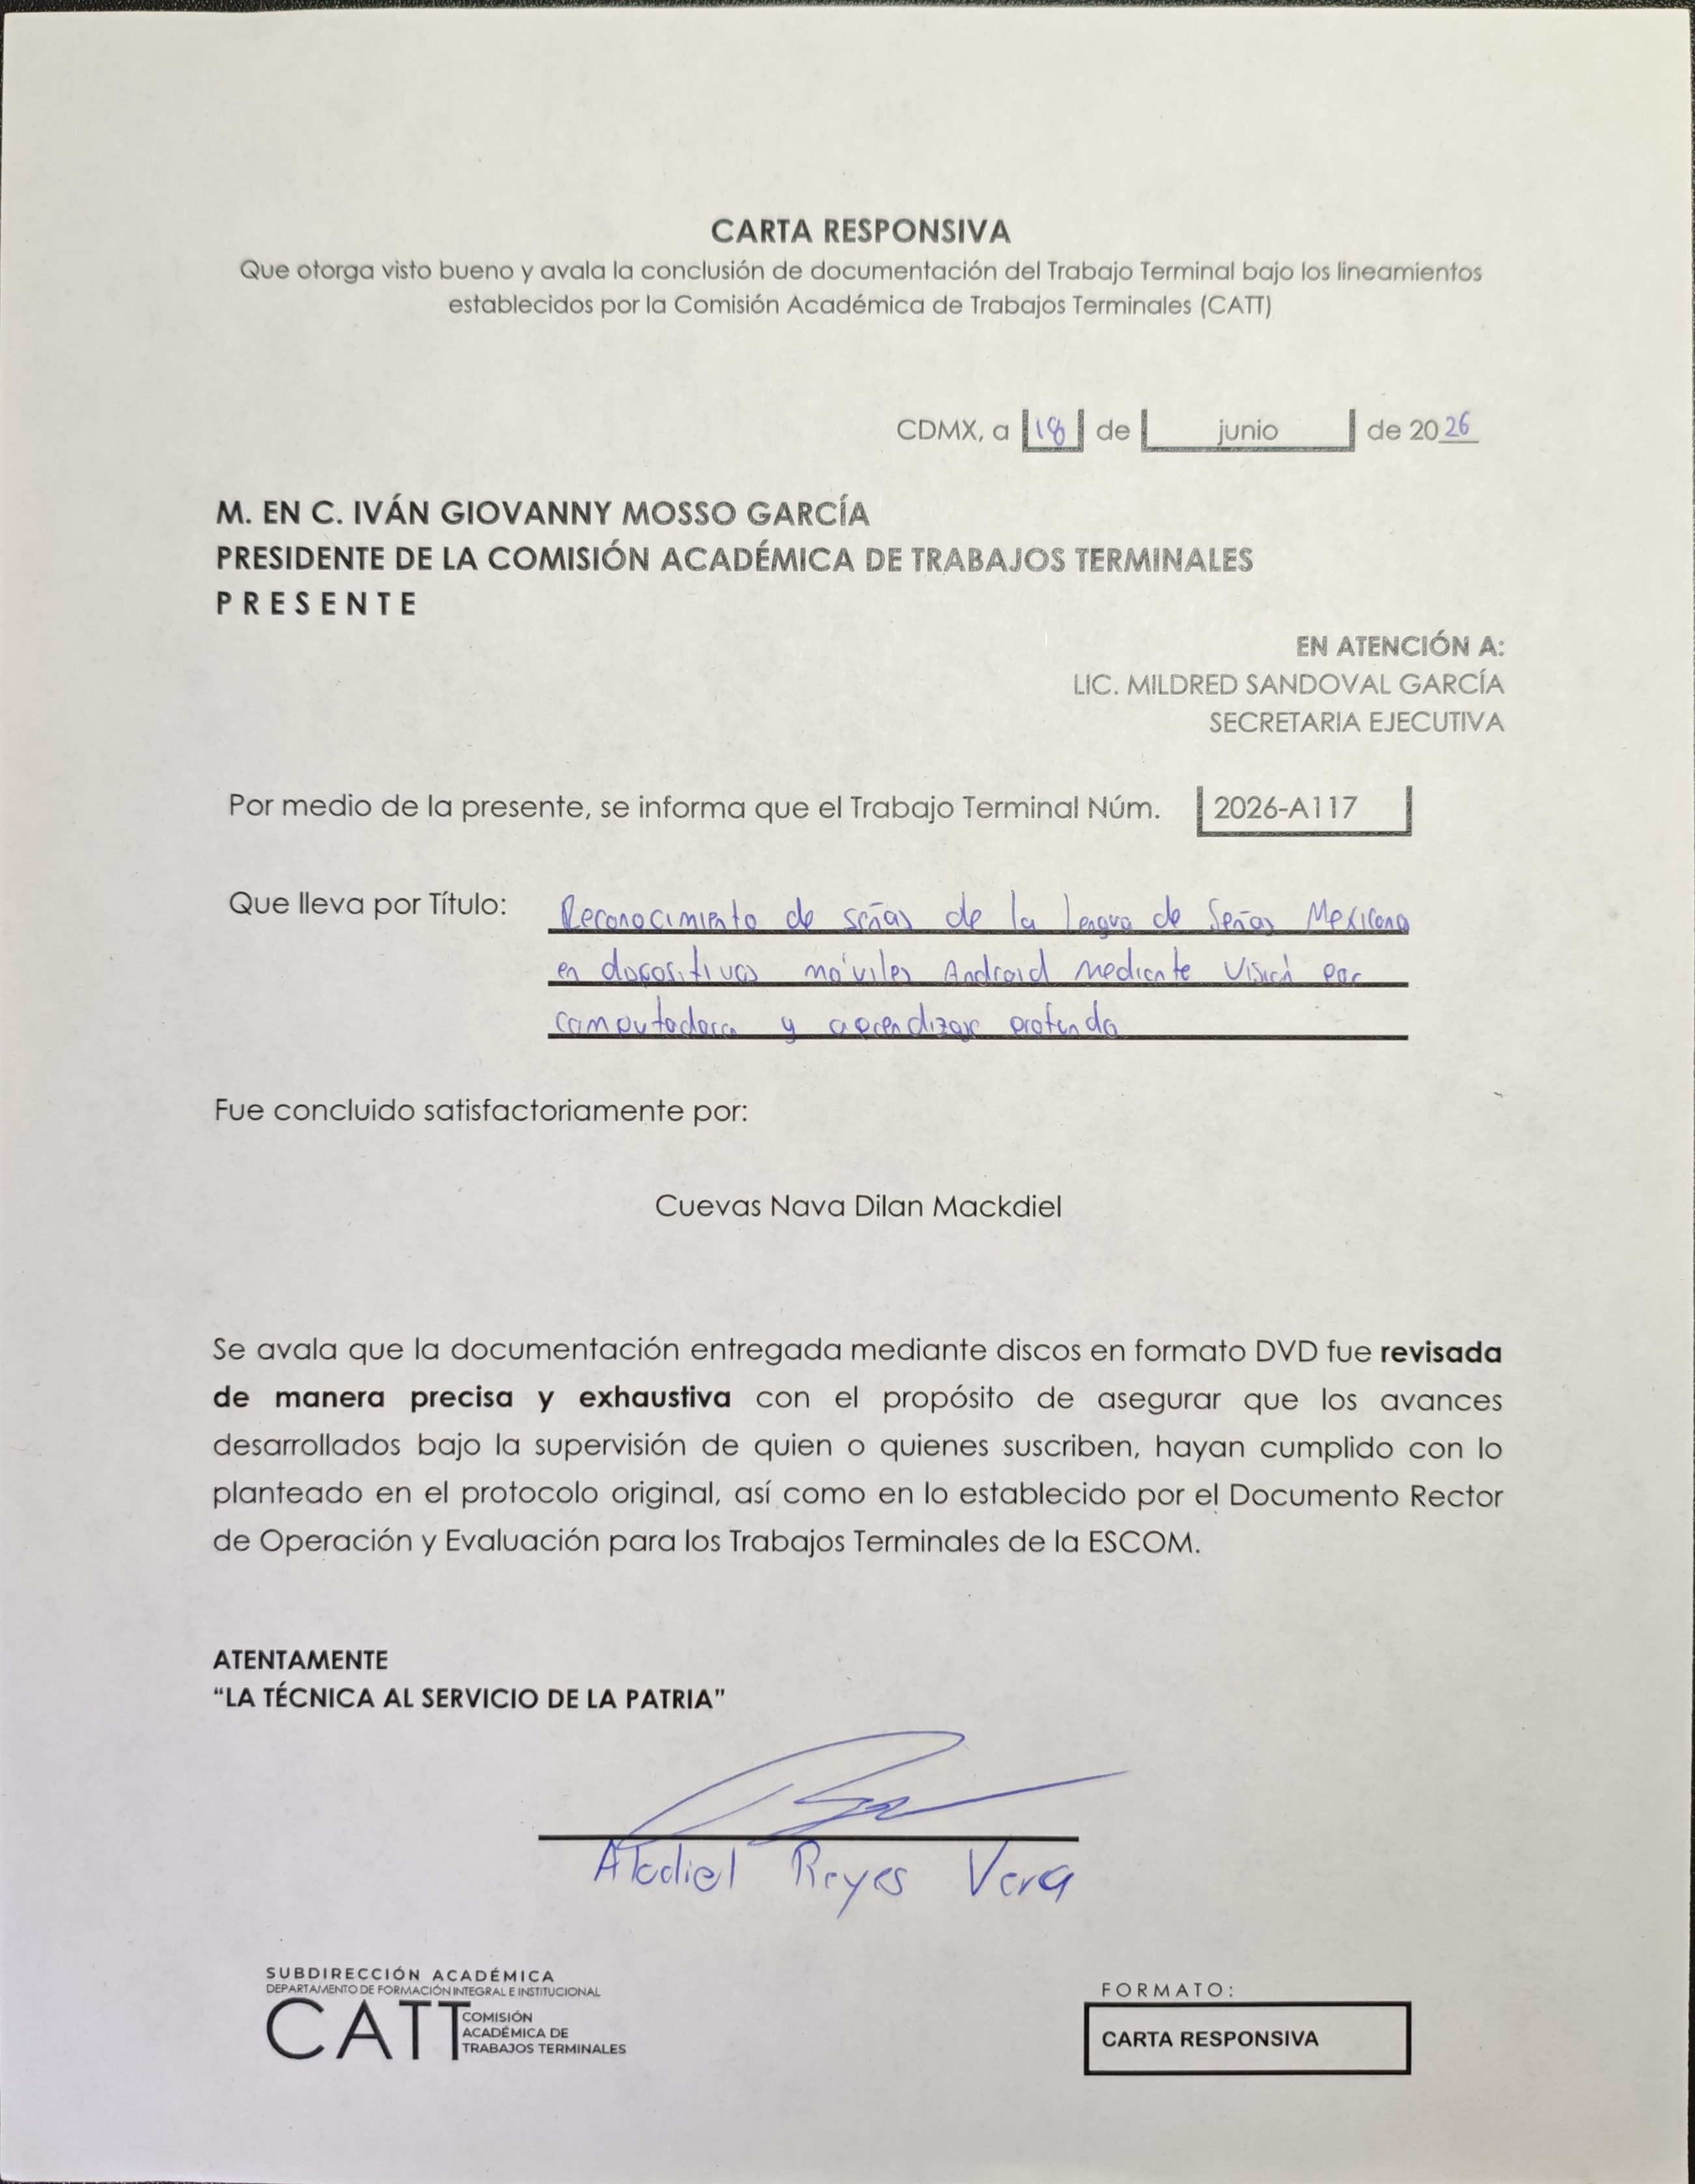
\includegraphics[
	%	width=\textwidth,
	%	height=\textheight,
	%	keepaspectratio
	%	]{images/cartaResponsiva.jpg}
	%\end{center}
	
	\cleardoublepage
	
		\cleardoublepage
	\thispagestyle{empty}
	
	\vspace*{\fill}
	
	\begin{center}
		\textbf{Advertencia}\\[0.5cm]
		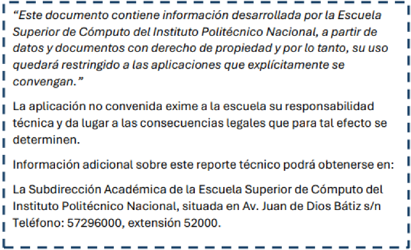
\includegraphics[width=0.75\textwidth]{images/advertencia.png}
	\end{center}
	
	\vspace*{\fill}
	
	
	% =========================
	% RESUMEN
	% =========================
	\cleardoublepage
	\thispagestyle{empty}
	
	\newpage
	
	% =========================
	% CARTA de autorizacion
	% =========================
	\cleardoublepage
	\thispagestyle{empty}
	
	%\begin{center}
	%	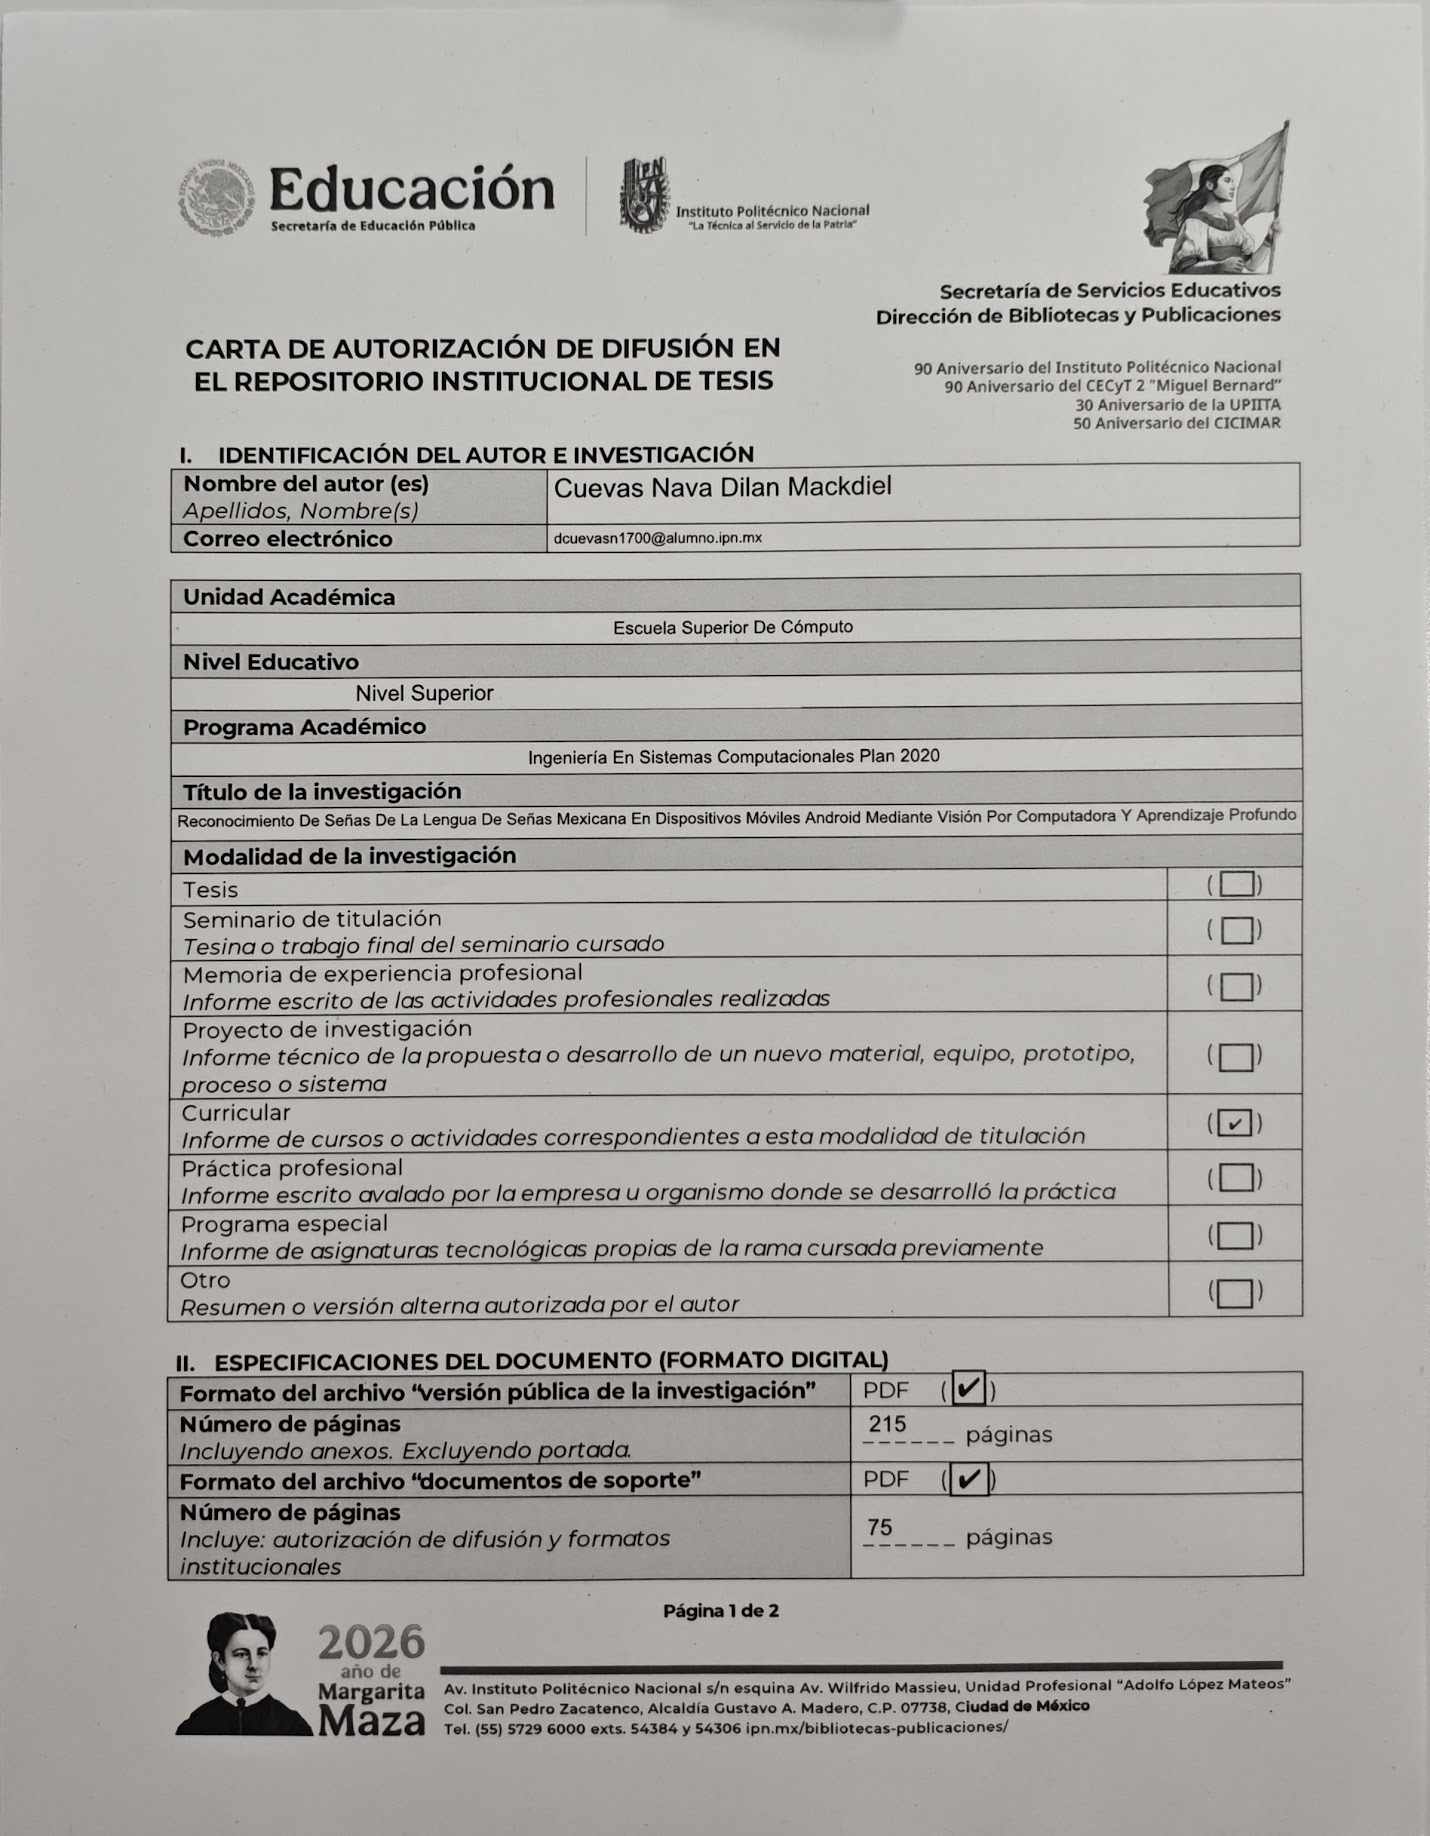
\includegraphics[
	%	width=\textwidth,
	%	height=\textheight,
	%	keepaspectratio
	%	]{images/cartaA1.jpg}
	%\end{center}
	
	\cleardoublepage

		\cleardoublepage
	\thispagestyle{empty}
	
	%\begin{center}
	%	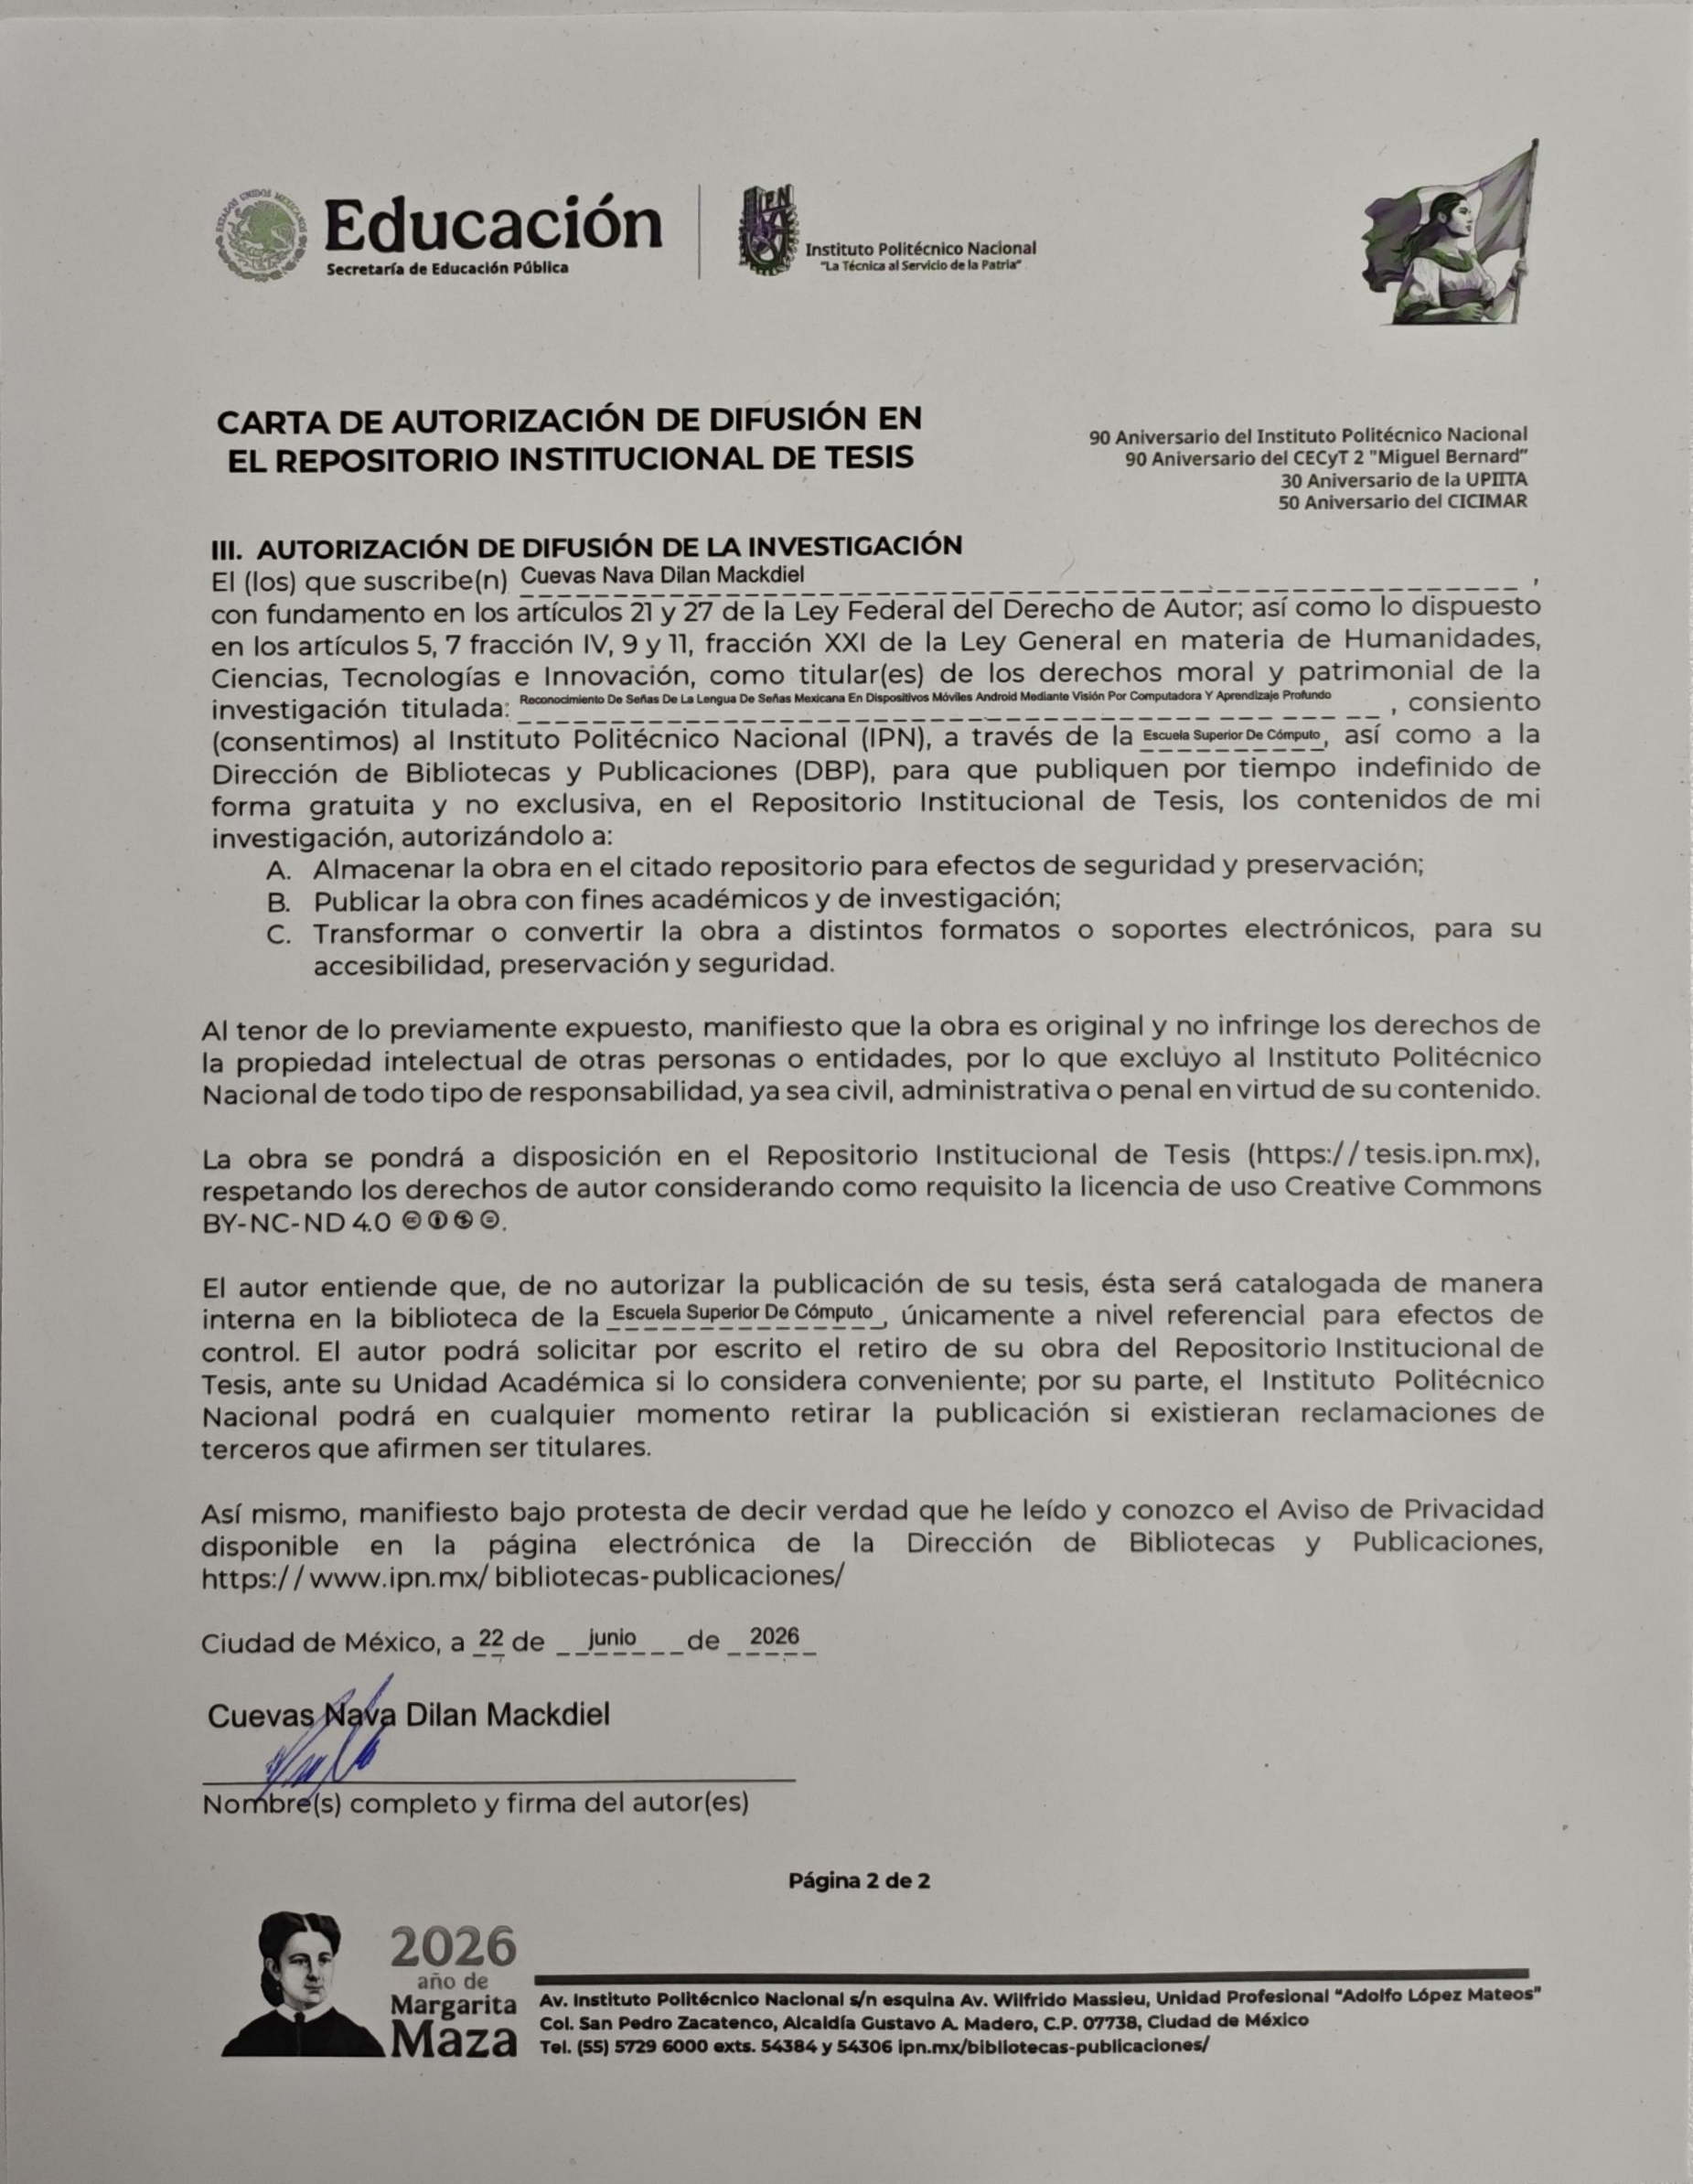
\includegraphics[
	%	width=\textwidth,
	%	height=\textheight,
	%	keepaspectratio
	%	]{images/cartaA2.jpg}
	%\end{center}
	
	\cleardoublepage
	

	\newpage
	

\cleardoublepage

%% Indice general, de figuras y de tablas
	% Numeración romana para preliminares
	
	% (\frontmatter: numeracion romana y capitulos sin numero)
	\frontmatter

	\tableofcontents

	\listoffigures

	\listoftables

	% Numeración arábiga para el contenido (\mainmatter empieza en pagina derecha)
	\mainmatter
	
	



% =========================
% CONTENIDO
% =========================
%% Introduccion
\section{Introducción}

El presente documento expone los avances del Trabajo Terminal 2026-B009, desarrollado en colaboración con la Defensoría de los Derechos Politécnicos (DDP) del Instituto Politécnico Nacional (IPN), cuyo propósito es diseñar e implementar una plataforma web que contribuya a optimizar los procesos de recepción, atención y seguimiento de quejas. Para ello, se analizan las necesidades operativas de la institución, las limitaciones de los procedimientos actuales y las alternativas tecnológicas que pueden contribuir a su mejora. La propuesta contempla la integración de herramientas de inteligencia artificial orientadas a la recuperación de antecedentes, la identificación de posibles duplicidades y la generación de resúmenes narrativos, como mecanismos de apoyo para las actividades del personal de la Defensoría.

El Instituto Politécnico Nacional (IPN) es una institución pública de educación media superior y superior que ofrece programas académicos en distintas áreas del conocimiento. Su organización, funcionamiento y atribuciones se encuentran regulados por disposiciones institucionales específicas que establecen su estructura y las funciones de sus órganos internos \cite{ipn_ley_organica}. En este marco institucional se encuentra la Defensoría de los Derechos Politécnicos, órgano encargado de promover, proteger y defender los derechos de la comunidad politécnica.

La Defensoría de los Derechos Politécnicos desempeña sus funciones dentro de la estructura institucional del IPN, de acuerdo con las atribuciones establecidas en su marco normativo \cite{ipn_acuerdo622, ipn_manual_organizacion_ddp}. Su actuación comprende actividades relacionadas con la orientación, recepción y atención de asuntos que involucran posibles vulneraciones de derechos. Si bien la DDP cuenta con atribuciones y funciones propias para el cumplimiento de sus responsabilidades, estas se desarrollan dentro del marco jurídico e institucional del IPN. El cumplimiento de dichas funciones requiere procedimientos que permitan administrar la información de manera organizada y dar seguimiento a las quejas presentadas por la comunidad politécnica.

Los procedimientos de atención de quejas de la DDP presentan áreas de oportunidad relacionadas con la digitalización y la organización de sus actividades internas. De acuerdo con el análisis de sus procesos y la documentación institucional, determinadas actividades de recepción, revisión y seguimiento requieren la intervención directa del personal responsable \cite{ipn_manual_procedimientos_ddp}. Esta dependencia puede incrementar la carga administrativa, dificultar la consulta de información y limitar la automatización de tareas repetitivas.

Asimismo, la revisión de las quejas requiere analizar los hechos descritos por los quejosos, consultar expedientes anteriores e identificar posibles coincidencias con casos previamente registrados. Estas actividades pueden demandar tiempo cuando la información se encuentra distribuida en distintos registros o cuando las descripciones presentan diferencias en su redacción. Por ello, resulta pertinente incorporar mecanismos tecnológicos que faciliten la recuperación de antecedentes, la identificación de posibles duplicidades y el énfasis en el contenido relevante de las quejas, además de apoyar la gestión y consulta de los expedientes.

La transformación digital ofrece alternativas para mejorar la administración de información y la ejecución de procesos institucionales. En el ámbito de la atención de quejas, las plataformas informáticas permiten centralizar registros, establecer mecanismos de seguimiento y controlar el acceso a información sensible. Sin embargo, la incorporación de tecnología no debe limitarse a sustituir documentos físicos por formularios electrónicos, sino que debe responder a las necesidades de los usuarios y a las características de los procedimientos existentes. Por esta razón, el desarrollo de una solución para la DDP requiere considerar tanto la gestión administrativa de los casos como las actividades de análisis que intervienen durante su atención.

A partir de las necesidades identificadas, el Trabajo Terminal propone el desarrollo de una plataforma web para administrar el proceso de atención de quejas dentro de la Defensoría. La solución contempla funcionalidades para el registro de quejas, la gestión de expedientes, el seguimiento de casos y la administración de usuarios conforme a sus responsabilidades institucionales. También considera la incorporación de herramientas que apoyen determinadas actividades de análisis y consulta de información. De esta manera, la plataforma busca integrar en un mismo entorno los componentes necesarios para facilitar la operación del personal y mantener organizada la información generada durante las distintas etapas de atención.

Uno de los componentes de inteligencia artificial del proyecto está orientado a la detección de posibles duplicidades y la recuperación de antecedentes mediante técnicas de Procesamiento de Lenguaje Natural (PLN). Este modelo analiza la similitud semántica entre una nueva queja y los expedientes previamente registrados, con el propósito de recuperar antecedentes relacionados e identificar posibles duplicidades que requieran una revisión posterior. Para ello, se emplean técnicas de representación vectorial de textos y recuperación de información que permiten comparar las descripciones de los hechos, incluso cuando se utilizan expresiones diferentes. Los resultados proporcionan al personal de la Defensoría una referencia para localizar antecedentes y reconocer posibles quejas duplicadas, sin sustituir la revisión necesaria para determinar si corresponden a un mismo caso.

El segundo componente de inteligencia artificial se enfoca en la generación automática de resúmenes narrativos a partir de las quejas presentadas por los integrantes de la comunidad politécnica. Su finalidad es transformar descripciones extensas, informales o poco estructuradas en textos concisos y coherentes que conserven los acontecimientos relevantes del relato original. Para ello, se consideran modelos de lenguaje capaces de procesar información textual y generar síntesis en lenguaje natural, estableciendo como criterios de evaluación la fidelidad al contenido original, la conservación de los hechos relevantes y la ausencia de información no sustentada en el relato del quejoso. Este componente busca facilitar la lectura de las quejas y enfatizar sus hechos principales, así como apoyar al personal responsable durante la revisión y documentación de los casos.

La plataforma contempla una arquitectura basada en microservicios para organizar sus funcionalidades en componentes independientes. Este enfoque permite separar responsabilidades, facilitar el mantenimiento y desarrollar modificaciones en determinados módulos sin intervenir directamente en la totalidad del sistema \cite{aws_microservicios, villamizar_microservices}. Entre los componentes considerados se encuentran el portal del quejoso, los módulos administrativos, la gestión de expedientes, los mecanismos de autenticación y autorización, y los servicios relacionados con el procesamiento de información mediante inteligencia artificial. La comunicación entre estos componentes requiere definir interfaces, reglas de acceso y mecanismos de intercambio de datos que permitan mantener la integridad y disponibilidad de la información.

El desarrollo del proyecto se apoya en el levantamiento y análisis de requerimientos realizado en colaboración con personal de la Defensoría. Mediante reuniones de trabajo y revisión de procedimientos institucionales, se identificaron actividades, responsabilidades y reglas de negocio relacionadas con la atención de quejas. Esta información permitió representar procesos mediante diagramas BPMN, elaborar propuestas de interfaces y diseñar estructuras de datos acordes con las necesidades identificadas. Asimismo, se realizaron actividades de implementación de componentes de backend y frontend, junto con pruebas funcionales y experimentales orientadas a revisar el comportamiento de las soluciones desarrolladas. Estos trabajos constituyen la base para continuar con la integración y validación de la plataforma.

La integración de herramientas digitales y de procesamiento de lenguaje natural constituye el enfoque tecnológico propuesto para atender las necesidades identificadas en la DDP. Se espera que la plataforma contribuya a organizar la información, facilitar el seguimiento de expedientes y proporcionar herramientas de apoyo para determinadas actividades administrativas y de análisis. No obstante, el alcance de estos beneficios deberá determinarse mediante las pruebas y evaluaciones correspondientes. En los capítulos siguientes se presentan los antecedentes, fundamentos teóricos, requerimientos, decisiones de diseño, actividades de implementación y procedimientos de evaluación que sustentan el desarrollo del Trabajo Terminal.

%% Planteamiento del Problema
	\section{Planteamiento del Problema}
	Este capítulo presenta el análisis de las principales problemáticas identificadas en los procesos
	actuales de atención y gestión de quejas dentro de la DDP. Se describen las causas que originan
	dichas limitaciones operativas y tecnológicas, así como la propuesta de solución planteada para
	optimizar la administración de expedientes, mejorar la trazabilidad de la información y fortalecer
	la eficiencia institucional mediante una plataforma digital integral.
	
	\subsection{Problema general}
	La gestión de quejas en la Defensoría de los Derechos Politécnicos (DDP) del Instituto Politécnico Nacional comprende un conjunto de procedimientos administrativos que requieren la participación de distintas áreas para la recepción, revisión, atención y seguimiento de las solicitudes presentadas por la comunidad politécnica. Estas actividades implican el manejo de información documental, la coordinación del personal responsable y el cumplimiento de las disposiciones institucionales que regulan la atención de los casos \cite{ipn_manual_procedimientos_ddp}.

	A partir del análisis de los procesos institucionales y del levantamiento de requerimientos realizado con personal de la Defensoría, se identificaron diversas dificultades operativas relacionadas con la administración, organización y seguimiento de las quejas. Estas situaciones afectan distintas actividades del procedimiento institucional y representan áreas de oportunidad para fortalecer la gestión de la información y la coordinación entre las áreas responsables. Su identificación permite establecer una visión general de las necesidades que deben atenderse para mejorar el funcionamiento de los procesos internos.

	El problema central radica en las limitaciones de los mecanismos actuales para gestionar de manera integral, organizada y eficiente los procedimientos relacionados con la atención de quejas. Esta situación representa un desafío para la operación, debido a la necesidad de mantener la continuidad de los expedientes, facilitar el acceso oportuno a la información y asegurar una coordinación adecuada durante las distintas etapas del procedimiento. Por ello, resulta necesario analizar las dificultades particulares que intervienen en la gestión de quejas y que, en conjunto, conforman la problemática identificada en la Defensoría.
	
	\subsection{Problemas específicos}
	La gestión de quejas en la Defensoría de los Derechos Politécnicos presenta diversas dificultades operativas que se manifiestan durante las etapas de recepción, revisión, atención y seguimiento de las solicitudes. A partir del levantamiento de requerimientos y del análisis de los procedimientos institucionales, se identificaron las siguientes problemáticas que afectan la organización de la información, la continuidad de los expedientes y las actividades del personal responsable.
	
	\begin{itemize}
		\item \textbf{Ausencia de una plataforma:} La administración de las quejas requiere mantener organizados los documentos, las evidencias y las actuaciones correspondientes a cada expediente. Durante este proceso se presentan dificultades para consultar y relacionar la información generada en las distintas etapas de atención, lo que puede incrementar el trabajo administrativo y complicar la recuperación de registros.

	
		\item \textbf{Seguimiento de las solicitudes:}
    El seguimiento de una queja implica conocer su estado, las actuaciones realizadas y las actividades pendientes. Las dificultades para consultar esta información de manera oportuna pueden afectar la continuidad del procedimiento y la coordinación entre las áreas responsables de su atención.

    \item \textbf{Carga operativa en las actividades administrativas:}
    El personal de la Defensoría realiza distintas actividades de registro, revisión, consulta y actualización de información durante la atención de quejas. Estas tareas requieren tiempo y atención constante, especialmente cuando deben gestionarse múltiples solicitudes de manera simultánea.

    \item \textbf{Revisión de narrativas extensas:}
    Algunas quejas presentadas por los integrantes de la comunidad politécnica contienen descripciones extensas de los acontecimientos. Su revisión requiere identificar los hechos relevantes, comprender la secuencia de los sucesos y reconocer la información necesaria para continuar con el procedimiento, lo que representa una actividad que demanda tiempo al personal responsable.

    \item \textbf{Presentación reiterada de quejas:}
    De acuerdo con lo señalado por el personal de la Defensoría, existen situaciones en las que los quejosos presentan nuevamente una solicitud relacionada con hechos previamente reportados, particularmente cuando consideran que no han recibido una respuesta. Esta situación puede generar registros potencialmente duplicados y requerir revisiones adicionales para determinar si corresponden a un expediente existente o contienen información nueva.

    \item \textbf{Consulta de antecedentes relacionados:}
    Durante la revisión de una queja puede ser necesario consultar expedientes anteriores relacionados con los hechos descritos o con las personas involucradas. La localización y comparación de estos registros representa una dificultad operativa, especialmente cuando existen diferencias en la manera de describir acontecimientos similares.

    \item \textbf{Coordinación entre las áreas responsables:}
    La atención de las quejas involucra la participación de diferentes áreas institucionales, cuyas actividades requieren mantener continuidad en el intercambio de información. Las dificultades para consultar las actuaciones y conocer el avance de los procedimientos pueden complicar la coordinación y el seguimiento de los casos.

    \item \textbf{Administración de información sensible:}
    Los expedientes pueden contener datos personales, documentos y descripciones de situaciones que requieren un tratamiento confidencial. Su administración representa un desafío debido a la necesidad de mantener la integridad de la información, controlar su consulta y conservar un registro de las actuaciones realizadas por el personal autorizado.

\end{itemize}

Estas problemáticas reflejan las dificultades que intervienen en la administración y atención de quejas dentro de la Defensoría. Aunque se manifiestan en distintas actividades del procedimiento, mantienen una relación directa con la organización de la información, la continuidad de los expedientes y la carga operativa del personal. Su análisis permite identificar los factores que contribuyen a su aparición, los cuales se desarrollan en el siguiente apartado.
	
	\subsection{Causas}
	Las problemáticas identificadas en la gestión de quejas de la Defensoría de los Derechos Politécnicos se relacionan con diversos factores administrativos, operativos y tecnológicos que intervienen en el desarrollo de sus procedimientos internos. A partir del análisis de los procesos institucionales y de la información obtenida durante el levantamiento de requerimientos, se reconocen condiciones que pueden contribuir a las dificultades de organización, consulta y seguimiento de los expedientes. Estos factores se encuentran relacionados entre sí, por lo que resulta necesario analizarlos desde una perspectiva integral.

	La dependencia de actividades manuales constituye uno de los factores que contribuyen a las dificultades operativas durante la atención de quejas. Los procedimientos institucionales requieren que el personal realice tareas de registro, revisión, actualización y consulta de información en distintas etapas del proceso \cite{ipn_manual_procedimientos_ddp}. Cuando estas actividades dependen principalmente de la intervención humana y carecen de mecanismos que faciliten su ejecución, el tiempo disponible del personal debe distribuirse entre tareas administrativas y actividades que requieren un análisis más detallado. Esta condición puede limitar la capacidad operativa de las áreas responsables, particularmente cuando deben atender varias solicitudes de manera simultánea.

	La integración limitada de la información representa otro factor que puede dificultar la continuidad de los procedimientos institucionales. La gestión de una queja involucra documentos, registros y actuaciones generados durante diferentes etapas de atención, cuya consulta requiere mantener una relación clara con el expediente correspondiente. Cuando la información se administra mediante mecanismos independientes o parcialmente integrados, resulta más complejo conservar una visión completa y actualizada del desarrollo de cada caso. Esta situación también puede dificultar el intercambio de información entre las áreas que participan en el procedimiento.

	Las características de las narrativas presentadas por los quejosos también influyen en el tiempo necesario para revisar las solicitudes. Debido a que los usuarios describen los acontecimientos desde su propia perspectiva, los escritos pueden variar considerablemente en extensión, estructura, claridad y nivel de detalle. Algunas narraciones incluyen información repetida, antecedentes extensos o acontecimientos que no siguen necesariamente un orden cronológico, lo que exige una lectura cuidadosa para identificar los hechos relevantes. La diversidad de estas características dificulta establecer un tiempo uniforme de revisión y aumenta la atención que debe dedicarse a determinados expedientes.

	La falta de mecanismos especializados para relacionar la información de diferentes expedientes puede contribuir a las dificultades para identificar antecedentes y posibles registros duplicados. Las solicitudes relacionadas con un mismo asunto no siempre presentan una redacción idéntica, debido a que los quejosos pueden describir nuevamente los acontecimientos utilizando expresiones diferentes o incorporando información adicional. Asimismo, distintos expedientes pueden compartir personas involucradas, circunstancias o características sin corresponder necesariamente al mismo hecho. Estas variaciones hacen que la identificación de relaciones entre registros requiera una comparación cuidadosa de su contenido y contexto.

	La comunicación y coordinación entre las áreas responsables constituye otro factor relevante en la gestión institucional de quejas. Durante el procedimiento pueden intervenir diferentes integrantes del personal, cada uno con funciones y responsabilidades específicas conforme a la organización de la Defensoría \cite{ipn_manual_organizacion_ddp}. La continuidad de las actuaciones depende de que la información generada en una etapa se encuentre disponible para quienes participan posteriormente. Por ello, los mecanismos utilizados para registrar, comunicar y consultar los avances de cada expediente influyen en la coordinación de las actividades institucionales.

	La naturaleza de la información administrada por la Defensoría establece condiciones particulares para su tratamiento y conservación. Los expedientes pueden contener datos personales, evidencias y descripciones de situaciones que requieren confidencialidad, por lo que su consulta debe realizarse conforme a las responsabilidades del personal autorizado. Esta necesidad exige mantener controles sobre el acceso, modificación y resguardo de los registros durante las distintas etapas del procedimiento. En consecuencia, la gestión de la información debe considerar tanto las necesidades operativas de la institución como las obligaciones relacionadas con su protección.

	En conjunto, los factores descritos permiten comprender las condiciones que contribuyen a las dificultades identificadas en los procesos de atención de quejas. Su relación evidencia que la problemática no se limita a una actividad particular, sino que involucra aspectos administrativos, documentales, organizacionales y tecnológicos. Este análisis proporciona una base para delimitar el alcance del Trabajo Terminal y establecer las funcionalidades que se contemplarán para atender las necesidades identificadas.
	

\subsection{Alcances}

El Trabajo Terminal 2026-B009 contempla el desarrollo de una plataforma web para la gestión de quejas de la Defensoría de los Derechos Politécnicos (DDP) del Instituto Politécnico Nacional. El sistema abarca los procesos de recepción, registro, revisión, atención y seguimiento de quejas, mediante la administración de expedientes digitales.

La plataforma contempla módulos diferenciados para los roles de quejoso, recepcionista, personal de primer contacto, subdefensor y defensor. Sus funcionalidades incluyen el registro de solicitudes, la administración de documentos y evidencias, el seguimiento de expedientes, las notificaciones y el historial de actuaciones, de acuerdo con los permisos correspondientes a cada usuario.

Como parte del sistema, se integran dos componentes de inteligencia artificial: un modelo de búsqueda de antecedentes y detección de posibles duplicidades mediante similitud semántica, y un modelo de generación de resúmenes narrativos que facilite la revisión de las quejas. Ambos funcionan como herramientas de apoyo para el personal de la Defensoría, sin sustituir su criterio ni las decisiones institucionales.

El desarrollo utiliza una arquitectura basada en microservicios e incorpora mecanismos de autenticación, autorización y control de acceso para proteger la información administrada. La plataforma está orientada a su utilización mediante navegadores web, sin contemplar el desarrollo de una aplicación móvil nativa ni la integración con sistemas externos al alcance definido.

El sistema no contempla la emisión automatizada de resoluciones o dictámenes jurídicos, ya que estas actividades corresponden exclusivamente al personal autorizado de la Defensoría.
	
	\subsection{Limitaciones}
	\label{sec:limitaciones}

	El desarrollo, implementación y evaluación del Trabajo Terminal están sujetos a restricciones académicas, tecnológicas e institucionales que pueden influir en el alcance y funcionamiento de la plataforma. Las principales limitaciones identificadas son las siguientes:

\begin{itemize}

    \item \textbf{Tiempo de desarrollo:} al tratarse de un proyecto académico con un periodo de ejecución definido, la implementación, integración y validación de los módulos se encuentran sujetas al calendario de entregas establecido. Por ello, algunas funcionalidades pueden permanecer en desarrollo durante las etapas intermedias del proyecto.

    \item \textbf{Disponibilidad de datos:} el desarrollo y la evaluación de los modelos de inteligencia artificial dependen de la disponibilidad de expedientes históricos. Ante las restricciones de acceso a información institucional sensible, se utilizan conjuntos de datos de prueba, por lo que los resultados obtenidos no necesariamente representan el comportamiento de los modelos ante casos reales de la Defensoría.

    \item \textbf{Precisión de los modelos:} la recuperación de antecedentes mediante similitud semántica puede identificar casos relacionados que no correspondan a una duplicidad real, así como omitir coincidencias relevantes. Por su parte, el modelo de generación de resúmenes puede presentar omisiones, interpretaciones incorrectas o información no sustentada en el texto original. En consecuencia, sus resultados requieren supervisión humana.

    \item \textbf{Infraestructura tecnológica:} el funcionamiento de la plataforma y de los modelos de inteligencia artificial depende de los recursos computacionales disponibles, particularmente de la capacidad de procesamiento, memoria y almacenamiento. Estas condiciones pueden limitar el rendimiento y la ejecución simultánea de determinados servicios.

    \item \textbf{Restricciones éticas y normativas:} el tratamiento de expedientes y datos personales debe ajustarse a las disposiciones institucionales y a la normativa aplicable en materia de protección de datos. Asimismo, los componentes de inteligencia artificial funcionan exclusivamente como herramientas de apoyo y no sustituyen la revisión, interpretación ni las decisiones jurídicas del personal autorizado.

\end{itemize}

%% Antecedentes
%\chapter{Estado del Arte}

En el Trabajo Terminal I (TT-I) se realizó un estudio comparativo de diversas plataformas nacionales e internacionales relacionadas con la recepción y gestión de denuncias, quejas y reportes institucionales. El análisis permitió identificar características funcionales y arquitectónicas relevantes, así como limitaciones presentes en soluciones gubernamentales, ciudadanas, corporativas y académicas. Este estudio sirvió como referencia para establecer los aspectos tecnológicos que debían considerarse en el diseño de la plataforma propuesta para la Defensoría de los Derechos Politécnicos (DDP).

Es importante distinguir entre los atributos considerados durante el análisis del estado del arte y los atributos que posteriormente fueron evaluados directamente en la plataforma desarrollada. Los primeros corresponden a características identificadas teóricamente a partir de la revisión de las soluciones existentes, mientras que los segundos forman parte de las evaluaciones y pruebas realizadas durante el desarrollo del presente Trabajo Terminal. Por lo tanto, la presencia de un atributo en el análisis comparativo no implica necesariamente que haya sido implementado o validado experimentalmente en la plataforma propuesta.

\section{Comparativa de plataformas}

A partir de los criterios definidos, se analizaron plataformas gubernamentales, ciudadanas, corporativas y académicas. Entre ellas se consideraron el Sistema Integral de Denuncias Ciudadanas (SIDEC), Denuncia Digital de la Ciudad de México, MP Virtual, Incorruptible, Sistema de Atención Mexiquense (SAM), Whistlelink, EQS Integrity Line, NAVEX/WhistleB, Whistleblower Software, BullyButton, Ventanilla Escolar, Alerta IPN y la plataforma de Denuncia en Línea de la UNAM. La comparación permitió identificar diferencias en aspectos como seguridad, anonimato, seguimiento, soporte multimedia, automatización, escalabilidad y adaptación al entorno universitario.

La Tabla~\ref{tab:comparativa_plataformas} resume los resultados obtenidos durante el análisis realizado en TT-I.

\rowcolors{2}{rowblue}{white}

\footnotesize

\renewcommand{\arraystretch}{1.2}

\setlength{\tabcolsep}{3pt}

\begin{longtable}{|L{2.9cm}|L{1.6cm}|L{1.7cm}|L{1.75cm}|L{1.6cm}|L{1.9cm}|L{1.75cm}|L{1.75cm}|}
    \caption{Comparativa general de plataformas de denuncia digital}
    \label{tab:comparativa_plataformas} \\
    \hline
    \rowcolor{headerblue}
    \headercell{Plataforma} &
    \headercell{Seguridad} &
    \headercell{Anoni\-mato} &
    \headercell{Segui\-miento} &
    \headercell{Multi\-media} &
    \headercell{Automati\-zación} &
    \headercell{Escala\-bilidad} &
    \headercell{Adaptación univer\-sitaria} \\
    \hline
    \endfirsthead
    \hline
    \rowcolor{headerblue}
    \headercell{Plataforma} &
    \headercell{Seguridad} &
    \headercell{Anoni\-mato} &
    \headercell{Segui\-miento} &
    \headercell{Multi\-media} &
    \headercell{Automati\-zación} &
    \headercell{Escala\-bilidad} &
    \headercell{Adaptación univer\-sitaria} \\
    \hline
    \endhead
    SIDEC & Media & Baja & Media & Sí & Baja & Media & No \\ \hline
    Denuncia Digital CDMX & Media & Baja & Media & Sí & Baja & Media & No \\ \hline
    MP Virtual & Media & Media & Media & Sí & Baja & Media & No \\ \hline
    Incorruptible & Baja & Media & Baja & Sí & Baja & Alta & No \\ \hline
    SAM & Media & Baja & Media & Sí & Baja & Media & No \\ \hline
    Whistlelink & Alta & Alta & Alta & Sí & Media & Alta & Parcial \\ \hline
    EQS Integrity Line & Alta & Alta & Alta & Sí & Alta & Alta & Parcial \\ \hline
    NAVEX / WhistleB & Alta & Alta & Alta & Sí & Alta & Alta & Parcial \\ \hline
    Whistleblower Software & Muy alta & Muy alta & Alta & Sí & Alta & Alta & Parcial \\ \hline
    BullyButton & Media & Media & Baja & Limitado & Baja & Media & Sí \\ \hline
    Ventanilla Escolar & Media & Baja & Baja & No & Baja & Media & Sí \\ \hline
    Alerta IPN & Media & Baja & Media & Sí & Baja & Media & Sí \\ \hline
    UNAM Denuncia en Línea & Media & Media & Alta & Sí & Media & Media & Sí \\ \hline
\end{longtable}

\normalsize

\setlength{\tabcolsep}{6pt}

\renewcommand{\arraystretch}{1}

\section{Brechas tecnológicas identificadas}

La comparación realizada en TT-I mostró que las plataformas analizadas presentan fortalezas en diferentes dimensiones, pero ninguna reúne de manera integral las características consideradas relevantes para el contexto de la DDP. Entre las principales brechas identificadas se encuentran la dependencia de arquitecturas centralizadas, la limitada automatización de procesos administrativos, las diferencias en los mecanismos de protección de identidad, la baja interoperabilidad entre servicios y las limitaciones para gestionar los expedientes de manera integral.

Asimismo, se observó una adaptación limitada de algunas soluciones a las necesidades particulares de instituciones universitarias públicas. Estas diferencias constituyeron un referente para definir las características de la solución propuesta, particularmente en aspectos relacionados con la organización de expedientes, el seguimiento de casos, la seguridad de la información y la incorporación de mecanismos de apoyo mediante inteligencia artificial.

El análisis del estado del arte permitió, por tanto, establecer un punto de referencia para el desarrollo de la plataforma de la DDP. Sin embargo, las características descritas corresponden al análisis comparativo realizado en TT-I y no deben interpretarse como resultados de pruebas efectuadas sobre la plataforma desarrollada en TT-II. La validación de los atributos que fueron implementados y seleccionados para evaluación se presenta posteriormente en los capítulos correspondientes.

%% Marco Teorico
	\section{Marco Teórico}
	Este capítulo reúne los fundamentos conceptuales sobre los que se sustenta la solución propuesta y
	se organiza en dos bloques. El primero desarrolla los principios arquitectónicos, las tecnologías de
	construcción y los mecanismos de seguridad sobre los que se edificó la plataforma web: diez
	microservicios en Java, cinco aplicaciones web en Angular, una base de datos PostgreSQL y una capa
	de publicación con proxy inverso y cifrado TLS, todo ejecutado en contenedores. El segundo bloque
	aborda los fundamentos del Procesamiento de Lenguaje Natural, las técnicas de representación y
	comparación de documentos, la recuperación de antecedentes y la generación automática de resúmenes
	narrativos. Estos componentes de inteligencia artificial se consideran herramientas de apoyo para la
	gestión de quejas y se integran dentro de la arquitectura general de la plataforma.

	\subsection{Fundamentos de arquitectura de software}
	\label{sec:arquitectura_software}
	La arquitectura de software es el conjunto de decisiones estructurales de alto nivel que definen
	cómo se organiza un sistema: qué componentes lo integran, qué responsabilidad tiene cada uno y cómo
	se comunican entre sí \cite{bbva_arquitectura_software}. Esas decisiones son costosas de revertir
	una vez que el sistema está en operación, de modo que conviene tomarlas de forma explícita y
	justificada desde el diseño, y no dejarlas al azar de la implementación. En una plataforma que
	acompaña un procedimiento institucional ---recepción, análisis, investigación y conclusión de una
	queja--- la arquitectura además debe reflejar la división de responsabilidades de la propia
	organización, porque cada área opera con datos, plazos y permisos distintos.

	\subsubsection{Atributos de calidad y el modelo ISO/IEC 25010}
	\label{sec:atributos_calidad}
	Una arquitectura no se evalúa únicamente por las funciones que permite construir, sino por los
	atributos de calidad que habilita o dificulta \cite{utel_atributos_calidad}. Para que esos atributos
	puedan especificarse y verificarse de manera uniforme, la norma ISO/IEC 25010 define un modelo de
	calidad del producto de software organizado en características y subcaracterísticas medibles
	\cite{iso25010}. El modelo sustituyó al de la norma ISO/IEC 9126 y es la referencia con la que en
	este trabajo se agrupan los requerimientos no funcionales (Capítulo~\ref{cap:analisis_diseno}) y
	las pruebas que los verifican (Capítulo~\ref{cap:pruebas}). La Tabla~\ref{tab:iso25010} resume las
	características que resultan pertinentes para una plataforma institucional de gestión de quejas.

	\rowcolors{2}{rowblue}{white}
	\small
	\renewcommand{\arraystretch}{1.25}
	\setlength{\tabcolsep}{5pt}
	\begin{longtable}{|p{3.0cm}|p{5.6cm}|p{5.4cm}|}
		\caption{Características de calidad de ISO/IEC 25010 aplicadas a la plataforma}
		\label{tab:iso25010} \\
		\hline
		\rowcolor{headerblue}
		\headercell{Característica} & \headercell{Definición} & \headercell{Pertinencia en la plataforma} \\
		\hline
		\endfirsthead
		\hline
		\rowcolor{headerblue}
		\headercell{Característica} & \headercell{Definición} & \headercell{Pertinencia en la plataforma} \\
		\hline
		\endhead
		Adecuación funcional & Grado en que el producto proporciona funciones completas, correctas y
		apropiadas para las tareas especificadas. & Las reglas del procedimiento (plazos, requisitos de
		admisión, estados del expediente) deben cumplirse sin excepción. \\ \hline
		Eficiencia de desempeño (capacidad) & Comportamiento temporal, uso de recursos y límites máximos
		que el producto soporta. & Recepción de evidencias de gran tamaño y atención simultánea de varias
		personas usuarias. \\ \hline
		Usabilidad & Facilidad con que usuarios específicos alcanzan sus objetivos con eficacia y
		satisfacción. & El quejoso es un usuario ocasional; el personal, uno intensivo. \\ \hline
		Fiabilidad & Capacidad de desempeñar funciones bajo condiciones especificadas, incluida la
		tolerancia a fallos y la recuperabilidad. & El fallo de un servicio auxiliar no debe impedir que
		una queja se registre; los datos deben poder restaurarse. \\ \hline
		Seguridad & Protección de la información para que personas o sistemas tengan el acceso que
		corresponde a su autorización. Incluye confidencialidad, integridad, no repudio, rendición de
		cuentas y autenticidad. & Las quejas identifican a personas y describen hechos; cada rol solo debe ver lo que le corresponde. \\ \hline
		Mantenibilidad & Eficacia con que el producto puede modificarse: modularidad, reusabilidad,
		analizabilidad, modificabilidad y capacidad de ser probado. & Las reglas normativas cambian; el
		equipo es reducido y el código debe poder entenderse y probarse. \\ \hline
		Compatibilidad y portabilidad & Capacidad de coexistir e intercambiar información con otros
		componentes y de instalarse en otros entornos. & Los servicios se comunican por interfaces
		estándar y se instalan con guiones reproducibles en servidores nuevos. \\ \hline
	\end{longtable}
	\normalsize
	\setlength{\tabcolsep}{6pt}
	\renewcommand{\arraystretch}{1}

	Dentro de la característica de seguridad, la \textbf{confidencialidad} ---que la información sea
	accesible solo para quien está autorizado--- merece un tratamiento propio en este trabajo, porque
	se verifica con un tipo distinto de prueba: no basta con revisar los permisos de cada punto de
	acceso, también debe comprobarse que la información no viaje legible por la red. Algo similar
	ocurre con la \textbf{capacidad}, subcaracterística de la eficiencia de desempeño que fija los
	límites máximos que el sistema debe soportar, como el tamaño de una petición o el número de
	usuarios concurrentes \cite{iso25010}. A estos atributos del modelo se suman otros dos que la
	operación de una defensoría vuelve imprescindibles: la \textbf{escalabilidad}, entendida como la
	capacidad de atender un volumen creciente de peticiones agregando recursos sin rediseñar el
	sistema \cite{microsoft_escalabilidad}, y la \textbf{trazabilidad}, es decir, la posibilidad de
	reconstruir qué ocurrió con cada expediente, quién intervino y cuándo, requisito tanto operativo
	como jurídico.

	\subsubsection{Del monolito a los microservicios}
	En una arquitectura \textbf{monolítica} toda la funcionalidad se empaqueta y despliega como una
	única unidad ejecutable \cite{ibm_monolitica}. Este enfoque es simple de desarrollar y desplegar en
	etapas tempranas, pero conforme el sistema crece presenta problemas conocidos: cualquier cambio
	obliga a reconstruir y desplegar la aplicación completa, el escalamiento debe hacerse en bloque
	aunque solo un componente esté saturado, y el acoplamiento interno dificulta que varias personas
	trabajen en paralelo sin interferir entre sí.

	Una arquitectura de \textbf{microservicios} descompone la aplicación en un conjunto de servicios
	pequeños e independientes, cada uno con una responsabilidad acotada, su propio ciclo de despliegue
	y una interfaz bien definida para comunicarse con los demás \cite{aws_microservicios}. La
	descomposición suele seguir las capacidades del negocio: cada servicio se alinea con una parte del
	dominio que tiene sentido por sí misma para la organización \cite{newman_microservices}. Cada
	servicio puede desarrollarse, desplegarse y escalarse por separado, lo que reduce el impacto de un
	cambio y permite dimensionar los recursos según la carga real de cada componente. La
	Tabla~\ref{tab:monolito_vs_microservicios} contrasta ambos estilos.

	\rowcolors{2}{rowblue}{white}
	\small
	\renewcommand{\arraystretch}{1.25}
	\setlength{\tabcolsep}{5pt}
	\begin{longtable}{|p{3.2cm}|p{5.4cm}|p{5.4cm}|}
		\caption{Comparación entre arquitectura monolítica y de microservicios}
		\label{tab:monolito_vs_microservicios} \\
		\hline
		\rowcolor{headerblue}
		\headercell{Criterio} & \headercell{Monolito} & \headercell{Microservicios} \\
		\hline
		\endfirsthead
		\hline
		\rowcolor{headerblue}
		\headercell{Criterio} & \headercell{Monolito} & \headercell{Microservicios} \\
		\hline
		\endhead
		Unidad de despliegue & La aplicación completa. & Cada servicio por separado. \\ \hline
		Escalamiento & En bloque, aunque solo un módulo lo requiera. & Selectivo, por servicio. \\ \hline
		Acoplamiento & Alto: los módulos comparten proceso y memoria. & Bajo: se comunican por
		interfaces explícitas. \\ \hline
		Impacto de un fallo & Puede detener toda la aplicación. & Acotado al servicio afectado si el
		diseño lo aísla. \\ \hline
		Complejidad operativa & Baja: un solo artefacto que administrar. & Alta: más artefactos, redes
		y puntos de fallo. \\ \hline
		Trabajo en equipo & Los cambios compiten sobre el mismo código. & Equipos independientes por
		servicio. \\ \hline
		Pruebas & Una sola suite, pero lenta y frágil conforme crece. & Suites pequeñas por servicio,
		más pruebas de integración entre ellos. \\ \hline
	\end{longtable}
	\normalsize
	\setlength{\tabcolsep}{6pt}
	\renewcommand{\arraystretch}{1}

	La elección entre ambos estilos no es absoluta. Estudios comparativos que despliegan una misma
	aplicación bajo los dos patrones muestran que los microservicios mejoran el aprovechamiento de
	recursos y la escalabilidad, pero a costa de una complejidad operativa considerablemente mayor
	\cite{villamizar_microservices}. Un sistema distribuido introduce problemas que un monolito no
	tiene ---latencia de red, fallos parciales, consistencia entre nodos--- y que deben resolverse de
	forma explícita \cite{tanenbaum_distribuidos}. Por esa razón existen posiciones intermedias, como
	mantener servicios independientes que comparten una única base de datos, de las que se trata en la
	Sección~\ref{sec:persistencia_datos}.

	\subsubsection{Arquitectura en capas}
	De forma transversal al estilo anterior, la organización interna de cada servicio suele seguir un
	esquema en capas, en el que la presentación, la lógica de negocio y el acceso a datos se separan en
	niveles con responsabilidades distintas \cite{ibm_tres_capas}. La capa de presentación expone la
	interfaz ---en un servicio web, los puntos de acceso HTTP, conocidos como \textit{controladores}---;
	la capa de negocio concentra las reglas del dominio en \textit{servicios}; y la capa de datos se
	ocupa de la persistencia mediante \textit{repositorios} y \textit{entidades}. Entre capas viajan
	objetos de transferencia de datos (DTO) que desacoplan el contrato externo de la estructura interna.
	La ventaja principal es que un cambio en una capa no obliga a modificar las demás mientras se
	respete el contrato entre ellas \cite{microsoft_ncapas}.

	Esta separación resulta especialmente valiosa cuando las reglas del dominio son normativas, como en
	el caso de una defensoría: al concentrarlas en una sola capa ---por ejemplo, en un paquete dedicado a
	validaciones---, un cambio en el reglamento se traduce en modificaciones localizadas y no dispersas
	por toda la aplicación \cite{coticolop_tres_capas}. Sobre esa base pueden además incorporarse
	políticas transversales ---control de acceso, registro de peticiones, manejo uniforme de errores---
	sin reescribir la lógica de negocio \cite{pozalujan_arquitectura}. La separación tiene también un
	efecto directo sobre la capacidad de ser probado: una regla que vive en un servicio sin dependencias
	de red ni de base de datos puede verificarse con pruebas unitarias rápidas y deterministas.

	\subsubsection{Comunicación entre servicios}
	Una vez dividido el sistema, sus partes deben comunicarse. Existen dos familias de mecanismos.

	La \textbf{comunicación síncrona} sigue el modelo petición-respuesta: un servicio llama a otro y
	espera el resultado antes de continuar. El estilo arquitectónico dominante para ello es REST
	(\textit{Representational State Transfer}), formulado por Fielding, que organiza la interfaz en
	torno a recursos identificados por URI y manipulados mediante los verbos del protocolo HTTP, con
	comunicación sin estado entre peticiones \cite{fielding_rest}. Su ventaja es la simplicidad
	conceptual y la interoperabilidad; su desventaja, que acopla temporalmente a los servicios, pues si
	el servicio invocado no responde, el invocador queda bloqueado o debe manejar el fallo. El contrato
	de una interfaz REST puede describirse de forma estándar y legible por máquina con la especificación
	OpenAPI, a partir de la cual se genera documentación navegable y clientes de prueba
	\cite{openapi_spec}.

	La \textbf{comunicación asíncrona} desacopla al emisor del receptor mediante colas o flujos de
	eventos: el servicio origen publica un evento y continúa, sin esperar a que alguien lo consuma
	\cite{stopford_event_driven}. Ofrece mayor tolerancia a fallos y mejor absorción de picos de carga,
	al precio de una complejidad notablemente mayor y de consistencia eventual en los datos.

	Cuando se opta por la comunicación síncrona, la literatura de sistemas en producción recomienda un
	conjunto de patrones de estabilidad para que el fallo de un servicio no se propague al resto
	\cite{nygard_release_it}. Los dos más elementales son los \textbf{tiempos de espera}
	(\textit{timeouts}), que impiden que una llamada sin respuesta retenga indefinidamente los recursos
	del invocador, y la \textbf{degradación controlada}, en la que una operación secundaria ---por
	ejemplo, enviar un correo de aviso--- se ejecuta en modo de mejor esfuerzo: si falla, se registra el
	error y la operación principal se completa de todos modos. Ambos patrones convierten un fallo
	parcial en un comportamiento predecible en lugar de una cascada de errores.

	Cuando el número de servicios crece, la comunicación directa entre ellos se vuelve difícil de
	administrar y aparecen componentes de apoyo ---registro y descubrimiento de servicios,
	configuración centralizada, balanceo de carga--- que resuelven de forma estándar esa
	infraestructura transversal \cite{spring_cloud}.

	\subsubsection{Persistencia de datos}
	\label{sec:persistencia_datos}
	La mayoría de los sistemas de información institucionales descansa sobre bases de datos
	relacionales, que organizan la información en tablas vinculadas por claves y garantizan las
	propiedades ACID: atomicidad, consistencia, aislamiento y durabilidad \cite{ibm_postgresql}. Esas
	garantías son especialmente pertinentes cuando cada registro corresponde a un expediente con
	efectos jurídicos, donde una escritura parcial o una lectura inconsistente no son aceptables. La
	atomicidad permite, además, resolver problemas de concurrencia sin mecanismos externos: una sola
	sentencia de actualización condicionada al estado actual de una fila se ejecuta de forma indivisible,
	de modo que si dos usuarios intentan apropiarse del mismo registro al mismo tiempo, solo uno lo
	consigue.

	PostgreSQL es un gestor relacional de código abierto ampliamente utilizado en producción, con
	soporte para tipos de datos binarios, transacciones concurrentes, índices avanzados y herramientas de
	respaldo y restauración lógica \cite{schonig_postgresql15}. Entre las aplicaciones y el gestor suele
	interponerse una capa de \textbf{mapeo objeto-relacional} (ORM), que traduce las clases del lenguaje
	de programación a tablas y genera las sentencias SQL; en el ecosistema Java el estándar es la
	especificación Jakarta Persistence (JPA), cuya implementación más difundida es Hibernate
	\cite{hibernate_orm}.

	En una arquitectura de microservicios la recomendación canónica es que cada servicio sea dueño
	exclusivo de sus datos (patrón \textit{base de datos por servicio}), para que ningún otro pueda
	acoplarse a su esquema \cite{richardson_microservices}. La alternativa, el patrón \textit{base de
	datos compartida}, permite que varios servicios lean y escriban en las mismas tablas: sacrifica
	autonomía de datos ---un cambio de esquema afecta a todos los servicios que lo usan--- a cambio de
	consultas directas entre dominios y de una operación más sencilla, compromiso que resulta razonable a
	escala institucional pequeña siempre que se documente qué servicio es dueño de cada tabla
	\cite{richardson_microservices, kleppmann_ddia}. Una consecuencia de cualquiera de los dos patrones
	es que la normalización estricta deja de ser el único criterio: es habitual que un servicio guarde
	una copia local de datos que pertenecen a otro ---el nombre de una persona junto a su identificador,
	por ejemplo--- para poder mostrarlos sin depender de una llamada en línea.

	\subsection{Tecnologías de construcción y ejecución}
	\label{sec:tecnologias}
	Definidos los principios arquitectónicos, esta sección describe las tecnologías concretas que los
	materializan, agrupadas por capa.

	\subsubsection{Plataforma del lado del servidor}
	Java es un lenguaje de programación orientado a objetos, compilado a un código intermedio que se
	ejecuta sobre una máquina virtual (JVM), lo que le da independencia respecto del sistema operativo
	subyacente \cite{oracle_java}. Su madurez, su tipado estático y su ecosistema de bibliotecas lo han
	consolidado en el desarrollo de sistemas empresariales de larga vida \cite{ibm_java}. Las versiones
	de soporte extendido (LTS), como Java 21, garantizan actualizaciones de seguridad durante varios
	años, condición deseable para un sistema institucional.

	Spring Boot es un marco de trabajo construido sobre el ecosistema Spring que reduce
	significativamente la configuración necesaria para levantar una aplicación: incorpora
	autoconfiguración, un servidor de aplicaciones embebido y un modelo de dependencias preempaquetadas
	que permite pasar de cero a un servicio operativo con poco código de infraestructura
	\cite{ibm_spring_boot}. A su alrededor se agrupan los módulos que una aplicación empresarial suele
	necesitar:

	\begin{itemize}
		\item \textbf{Spring Data JPA}, que genera los repositorios de acceso a datos a partir de
		interfaces y delega el mapeo en Hibernate \cite{hibernate_orm}.
		\item \textbf{Spring Security}, que intercepta cada petición en una cadena de filtros donde se
		autentica al usuario y se evalúan las reglas de autorización, tanto por ruta como por método
		mediante anotaciones \cite{spring_security_ref}.
		\item \textbf{Clientes HTTP declarativos} (OpenFeign) y de plantilla (\texttt{RestTemplate}),
		con los que un servicio invoca a otro como si llamara a un método local.
		\item \textbf{springdoc-openapi}, que inspecciona los controladores y publica su contrato
		OpenAPI junto con una interfaz navegable \cite{openapi_spec}.
	\end{itemize}

	Spring Boot ofrece además componentes para exponer el estado interno de la aplicación ---métricas,
	verificaciones de salud, información de entorno--- indispensables para operar un sistema
	distribuido sin acceso directo a un depurador \cite{alvarezcaules_actuator}. La construcción de los
	artefactos se automatiza con Apache Maven, que resuelve las dependencias declaradas en un archivo de
	proyecto, compila, ejecuta las pruebas y empaqueta cada servicio como un archivo \texttt{.jar}
	autoejecutable \cite{maven_ref}.

	Para el desarrollo de los componentes de inteligencia artificial se emplea también Python, un
	lenguaje de programación de propósito general que dispone de bibliotecas especializadas en
	Procesamiento de Lenguaje Natural, recuperación de información y aprendizaje automático
	\cite{aws_python}, y que cuenta con marcos ligeros para publicar esos componentes como servicios
	web. Los fundamentos de dichos componentes se desarrollan a partir de la
	Sección~\ref{sec:busqueda_antecedentes}.

	\subsubsection{Interfaz de usuario}
	Angular es un marco de trabajo para construir aplicaciones web de página única (\textit{single-page
	applications}), en las que la navegación ocurre en el navegador sin recargar el documento completo
	\cite{angular_overview}. Está organizado en componentes reutilizables que encapsulan plantilla,
	estilos y lógica, e incorpora de forma nativa enrutamiento, gestión de formularios, cliente HTTP e
	inyección de dependencias, lo que evita ensamblar esas piezas a partir de bibliotecas sueltas
	\cite{imagina_angular}. Las versiones recientes del marco introdujeron tres cambios relevantes para
	este trabajo \cite{angular_signals}:

	\begin{itemize}
		\item \textbf{Componentes independientes} (\textit{standalone}), que declaran directamente sus
		dependencias sin agruparse en módulos, lo que simplifica la estructura del proyecto.
		\item \textbf{Señales} (\textit{signals}), valores reactivos que notifican a la vista cuándo
		cambian, y el modo de \textbf{detección de cambios sin zonas} (\textit{zoneless}), en el que la
		interfaz se actualiza solo cuando una señal cambia o cuando se solicita de forma explícita.
		\item \textbf{Carga diferida} de rutas y bloques de plantilla, con la que cada pantalla se
		descarga la primera vez que se visita y no como parte del paquete inicial.
	\end{itemize}

	El resultado de la compilación es un conjunto de archivos estáticos ---HTML, CSS y JavaScript--- que
	cualquier servidor web puede entregar, sin necesidad de ejecutar código del lado del servidor para la
	interfaz. Las aplicaciones Angular controlan el acceso a sus rutas mediante \textit{guardas}, funciones
	que deciden si una navegación procede, e intervienen en las peticiones HTTP mediante
	\textit{interceptores}, que permiten, por ejemplo, adjuntar a todas ellas el token de sesión.

	\subsubsection{Contenedores}
	Un contenedor empaqueta una aplicación junto con todas sus dependencias en una unidad aislada que
	se ejecuta sobre el núcleo del sistema operativo anfitrión \cite{redhat_docker}. A diferencia de
	una máquina virtual, no incluye un sistema operativo completo, por lo que arranca en segundos y
	consume una fracción de los recursos. Su aporte principal es la reproducibilidad: la misma imagen
	se ejecuta de forma idéntica en la máquina de desarrollo y en el servidor de producción, lo que
	elimina toda una clase de fallos atribuibles a diferencias de entorno. Los contenedores admiten
	además límites explícitos de memoria y procesador, y políticas de reinicio automático que los
	vuelven a levantar si terminan de forma inesperada o si el servidor se reinicia.

	Podman es un motor de contenedores compatible con el formato de imágenes OCI y con la línea de
	comandos de Docker, que se distingue por no depender de un proceso servidor residente: cada
	contenedor es un proceso hijo del usuario que lo ejecuta \cite{podman_docs}. Esa característica
	reduce la superficie de ataque del anfitrión. Una particularidad que conviene conocer es que, al
	publicar un puerto, tanto Podman como Docker insertan reglas de traducción de direcciones en el
	cortafuegos del núcleo que se evalúan antes que las de herramientas de alto nivel como
	\texttt{ufw}; en consecuencia, restringir un puerto publicado exige reglas propias en etapas
	anteriores del filtrado de paquetes.

	Los contenedores son, además, la unidad natural de despliegue de una arquitectura de
	microservicios: cada servicio se distribuye como una imagen propia, versionada e inmutable. Cuando
	el número de contenedores crece hasta volverse inmanejable manualmente, se recurre a plataformas de
	orquestación que automatizan su ciclo de vida, la recuperación ante fallos y el escalamiento
	\cite{burns_kubernetes}; a escalas menores, esa administración puede resolverse con guiones de
	despliegue, opción suficiente cuando el número de servicios es moderado y el equipo pequeño.

	\subsubsection{Proxy inverso}
	Un proxy inverso es un servidor que se coloca frente a uno o varios servicios y recibe en su nombre
	todas las peticiones del exterior, para después reenviarlas al componente que corresponda según la
	ruta solicitada \cite{nginx_org}. Concentra en un solo punto responsabilidades que de otro modo
	habría que replicar en cada servicio: terminación de conexiones cifradas, balanceo de carga,
	entrega de contenido estático, compresión, políticas de caché, límites de tamaño de las peticiones y
	control del tráfico entrante \cite{khanal2023nginx}.

	Su papel es doble en una aplicación web moderna. Por un lado entrega los archivos estáticos que
	componen la interfaz; por otro, enruta las peticiones dirigidas a la API hacia el servicio
	correspondiente. Desde el punto de vista del navegador todo proviene de un mismo origen, lo que
	simplifica el modelo de seguridad del cliente, mientras que del lado del servidor la separación en
	servicios permanece intacta. Al ser el único punto expuesto a Internet, el proxy es también el lugar
	natural para bloquear rutas que solo deben invocarse entre servicios internos.

	\subsection{Seguridad aplicada al software}
	\label{sec:seguridad_software}
	Una plataforma que administra quejas maneja, por definición, información sensible: identifica a
	quien denuncia, a quien es señalado y describe hechos que pueden tener consecuencias
	disciplinarias o jurídicas. Los mecanismos de esta sección son, por ello, requisitos del sistema y
	no características opcionales. Como referencia de los riesgos que deben atenderse se toma la lista
	OWASP Top 10, que reúne las categorías de vulnerabilidad más frecuentes en aplicaciones web; en su
	edición de 2021 encabezan la lista el control de acceso defectuoso, las fallas criptográficas y la
	inyección, y el control de acceso conserva el primer lugar en la revisión posterior \cite{owasp_top10}. Cada una de las subsecciones siguientes atiende alguno de esos riesgos.

	\subsubsection{Autenticación basada en tokens}
	En una arquitectura distribuida, mantener la sesión del usuario en la memoria del servidor obliga a
	que todas sus peticiones lleguen siempre a la misma instancia, lo que limita el escalamiento
	horizontal. La alternativa es la autenticación basada en tokens: el servicio de autenticación
	verifica las credenciales una sola vez y emite un token firmado que el cliente adjunta en cada
	petición posterior, normalmente en el encabezado \texttt{Authorization} con el esquema
	\texttt{Bearer}.

	JSON Web Token (JWT) es el formato más extendido para ello \cite{rfc7519}. Se compone de tres
	partes ---encabezado, carga útil y firma--- codificadas y separadas por puntos. La carga útil contiene
	afirmaciones (\textit{claims}) sobre el usuario, como su identidad, su rol, la fecha de emisión
	(\texttt{iat}) y la de expiración (\texttt{exp}); la firma, calculada con una clave secreta mediante
	un algoritmo como HMAC-SHA256 (HS256), permite a cualquier servicio que la conozca verificar que el
	contenido no fue alterado \cite{spring_security_jwt}. Su propiedad más útil en un sistema
	distribuido es que la validación es local: un servicio puede autorizar una petición sin consultar al
	servicio emisor ni mantener estado de sesión compartido. Con una firma simétrica, todos los servicios
	que validan comparten el mismo secreto, por lo que su resguardo ---fuera del código fuente y del
	repositorio--- es parte crítica del diseño.

	Esa misma propiedad tiene un costo: al ser autocontenido, un token válido no puede revocarse antes
	de su expiración sin introducir un mecanismo adicional de listas de revocación. De ahí que se
	recomiende emitirlos con tiempos de vida cortos y que el cliente descarte la sesión en cuanto el
	servidor rechace el token. Transmitir el token en un encabezado, y no en una \textit{cookie}, tiene
	la ventaja adicional de que el navegador no lo envía de forma automática, lo que elimina la clase
	de ataques de falsificación de peticiones entre sitios (CSRF).

	\subsubsection{Almacenamiento seguro de contraseñas}
	Las contraseñas nunca deben almacenarse en texto plano ni cifradas de forma reversible, pues quien
	obtenga acceso a la base de datos obtendría también las credenciales de todos los usuarios. La
	práctica correcta es guardar el resultado de una función resumen (\textit{hash}) diseñada
	específicamente para este fin, que sea deliberadamente costosa de calcular y que incorpore un valor
	aleatorio distinto por usuario (\textit{salt}), de modo que dos usuarios con la misma contraseña
	produzcan resúmenes diferentes y no puedan emplearse tablas precalculadas para revertirlos
	\cite{owasp_password_storage}. BCrypt, derivada del cifrado Blowfish, es una de las funciones
	recomendadas: incluye el \textit{salt} en el propio valor almacenado y un factor de costo ajustable
	que permite aumentar su dificultad conforme crece la capacidad de cómputo \cite{provos_bcrypt}. La
	verificación en el inicio de sesión no consiste entonces en descifrar el valor almacenado, sino en
	recalcular el resumen de la contraseña recibida y compararlo con el registrado.

	El mismo principio aplica a cualquier secreto de un solo uso, como un código de recuperación de
	contraseña: se guarda su resumen y no el valor, se le asigna una vigencia corta y se limita el número
	de intentos de verificación, para que no pueda adivinarse por fuerza bruta \cite{nist_80063b}.

	\subsubsection{Control de acceso basado en roles}
	La autenticación resuelve quién es el usuario; la autorización, qué le está permitido hacer. El
	control de acceso basado en roles (RBAC) asigna a cada usuario uno o varios roles y asocia los
	permisos a esos roles y no a las personas, lo que simplifica la administración y reduce el riesgo de
	conceder privilegios por olvido \cite{sandhu_rbac}. Debe aplicarse siguiendo el principio de menor
	privilegio: cada rol recibe únicamente los permisos indispensables para su función, y cada punto de
	acceso declara de forma explícita qué rol puede invocarlo. En una defensoría, esa distinción es
	también organizativa: quien recibe una queja no debe poder emitir un dictamen, ni quien investiga
	puede modificar la recepción.

	El control por rol no basta por sí solo. Cuando un recurso pertenece a una persona ---una queja, una
	notificación, un acuerdo---, el servidor debe comprobar además que quien lo solicita es su dueño, y
	hacerlo con la identidad contenida en el token, nunca con un identificador enviado por el cliente.
	Omitir esa verificación produce la vulnerabilidad conocida como referencia directa insegura a
	objetos, en la que basta con cambiar un folio en la URL para consultar el expediente de otra persona
	\cite{owasp_top10}. Por la misma razón, las reglas de negocio deben validarse en el servidor y no solo
	en la interfaz: ocultar un botón no impide que alguien invoque directamente el punto de acceso.

	\subsubsection{Cifrado en tránsito}
	Toda la información que viaja entre el navegador y el servidor debe protegerse con TLS
	(\textit{Transport Layer Security}), protocolo que establece un canal cifrado y autenticado sobre
	una conexión de red no confiable. Su versión 1.3 simplificó el proceso de negociación, redujo la
	latencia de establecimiento de la conexión y eliminó los algoritmos criptográficos considerados
	inseguros en versiones previas \cite{rescorla_tls13}; las versiones 1.0 y 1.1 se consideran
	obsoletas y no deben aceptarse. La autenticidad del servidor se garantiza con un certificado emitido
	por una autoridad reconocida; Let's Encrypt emite certificados gratuitos de vigencia corta mediante
	el protocolo automatizado ACME, de modo que su renovación puede programarse sin intervención humana
	\cite{letsencrypt}.

	El cifrado se complementa con medidas de configuración del servidor. El encabezado
	\texttt{Strict-Transport-Security} (HSTS) indica al navegador que el sitio solo debe visitarse por
	HTTPS, lo que evita que un atacante degrade la primera conexión a HTTP \cite{rfc6797}. Y la
	compresión de respuestas que mezclan secretos con datos controlados por el usuario debe evitarse,
	porque el tamaño de la respuesta comprimida puede filtrar información aun cuando el canal esté
	cifrado ---la familia de ataques conocida como BREACH---. Sin estas medidas, las credenciales, los
	tokens de sesión y el contenido íntegro de una denuncia quedarían expuestos a cualquier intermediario
	de la red.

\subsection{Fundamentos de Procesamiento de Lenguaje Natural}
El Procesamiento de Lenguaje Natural (PLN) es una rama de la inteligencia artificial que estudia los métodos mediante los cuales las computadoras pueden analizar, interpretar y generar información expresada en lenguaje humano \cite{jurafsky2023slp}. Sus aplicaciones incluyen la recuperación de información, el análisis de documentos y la generación automática de resúmenes, tareas que requieren procesar el contenido lingüístico de los textos.

Una de las principales dificultades del PLN es la naturaleza ambigua y contextual del lenguaje. Una misma idea puede expresarse mediante palabras diferentes, mientras que expresiones similares pueden adquirir significados distintos según las circunstancias en las que se utilizan. Por ello, el procesamiento computacional debe considerar tanto las características lingüísticas del texto como las relaciones semánticas que permiten interpretar su contenido.

En el contexto de la Defensoría de los Derechos Politécnicos (DDP), las quejas se presentan mediante narrativas que pueden variar en extensión, estructura y vocabulario. Estas características hacen necesario emplear técnicas que permitan representar su contenido, establecer relaciones entre documentos y procesar la información descrita. Los fundamentos de estas técnicas comprenden el preprocesamiento lingüístico y la representación vectorial del texto, que se desarrollan a continuación.

\subsubsection{Preprocesamiento de textos}

El preprocesamiento consiste en preparar el contenido textual para su análisis mediante técnicas computacionales. Su propósito es identificar las unidades lingüísticas relevantes y, cuando resulta necesario, reducir variaciones que puedan dificultar la comparación entre documentos. Entre las operaciones más utilizadas se encuentran la tokenización, la lematización y el tratamiento de palabras vacías \cite{jurafsky2023slp}.

\paragraph{Tokenización.}

La tokenización divide un texto en unidades denominadas \textit{tokens}, que pueden corresponder a palabras, signos de puntuación u otros elementos lingüísticos. Esta operación permite identificar los componentes de una oración para su posterior análisis.

Por ejemplo, la expresión ``El profesor negó el acceso'' puede dividirse en los siguientes tokens:

\begin{center}
    [\texttt{El}, \texttt{profesor}, \texttt{negó},
    \texttt{el}, \texttt{acceso}]
\end{center}

\paragraph{Lematización.}

La lematización consiste en reducir las palabras a su forma canónica o lema, considerando sus características morfológicas. Esta transformación permite relacionar distintas formas de una misma palabra y disminuir las variaciones presentes en los documentos \cite{jurafsky2023slp}.

Por ejemplo:

\begin{center}
    \texttt{negaron} $\rightarrow$ \texttt{negar}
\end{center}

\begin{center}
    \texttt{estudiantes} $\rightarrow$ \texttt{estudiante}
\end{center}

\paragraph{Tratamiento de palabras vacías.}

Las palabras vacías, conocidas como \textit{stop words}, son términos frecuentes que, dependiendo de la tarea, pueden aportar poca información para distinguir documentos. Entre ellas se encuentran determinados artículos, preposiciones y conjunciones.

Sin embargo, su eliminación debe realizarse cuidadosamente, ya que expresiones como ``no'', ``sin'' y ``nunca'' pueden modificar el significado de los acontecimientos descritos en una queja. Por esta razón, el preprocesamiento debe considerar las características del contenido y los requisitos del modelo utilizado.

Estas operaciones constituyen herramientas para preparar los textos, aunque no necesariamente deben aplicarse todas ni en el mismo orden. Su selección depende del método de representación y del tipo de análisis que se pretende realizar.


\subsubsection{Representación vectorial del texto}

La representación vectorial permite transformar documentos escritos en estructuras numéricas que pueden procesarse mediante algoritmos computacionales. Cada texto se representa mediante un vector cuyas dimensiones contienen información sobre sus características lingüísticas o semánticas. Esta transformación constituye el fundamento de los métodos que comparan documentos y recuperan información relacionada \cite{manning2008ir}.

Las técnicas de representación textual pueden distinguirse entre enfoques estadísticos, que consideran principalmente la presencia y frecuencia de términos, y enfoques basados en \textit{embeddings}, que buscan representar relaciones semánticas entre palabras, oraciones o documentos.

\paragraph{Bolsa de palabras y TF-IDF.}

El modelo de bolsa de palabras, conocido como \textit{Bag of Words} (BoW), representa un documento mediante la frecuencia de aparición de sus términos, sin considerar el orden en el que se presentan. Aunque permite comparar documentos a partir de su vocabulario, no representa directamente las relaciones de significado entre las palabras \cite{manning2008ir}.

Una extensión de este enfoque es TF-IDF (\textit{Term Frequency--Inverse Document Frequency}), que asigna un peso a cada término considerando su frecuencia dentro de un documento y su presencia en el conjunto de documentos.

Su expresión general es:

\begin{equation}
    \operatorname{tf-idf}(t,d,D)
    =
    \operatorname{tf}(t,d)
    \times
    \operatorname{idf}(t,D)
    \label{eq:tfidf}
\end{equation}

donde $t$ representa un término, $d$ un documento y $D$ el conjunto de documentos. El componente TF mide la frecuencia del término dentro del documento, mientras que IDF reduce la importancia de los términos que aparecen en numerosos documentos \cite{manning2008ir}.

TF-IDF resulta útil para identificar coincidencias léxicas entre textos. Sin embargo, presenta limitaciones cuando dos documentos describen acontecimientos similares utilizando vocabulario diferente. Esta característica motiva el uso de representaciones capaces de incorporar información semántica.

\paragraph{Embeddings de palabras.}
Los \textit{word embeddings} representan palabras mediante vectores numéricos densos, obtenidos a partir de patrones de uso observados durante el entrenamiento de modelos lingüísticos. Su fundamento consiste en que las palabras utilizadas en contextos semejantes pueden adquirir representaciones cercanas dentro de un espacio vectorial \cite{mikolov2013word2vec}.

A diferencia de los modelos basados únicamente en frecuencias, estas representaciones permiten establecer relaciones entre términos que no necesariamente comparten la misma escritura. Por ejemplo, palabras como ``hostigamiento'' y ``acoso'' pueden presentar proximidad en el espacio vectorial debido a sus relaciones semánticas.

Herramientas como spaCy proporcionan modelos lingüísticos que incluyen representaciones vectoriales y funcionalidades para el procesamiento de textos \cite{honnibal2020spacy}. No obstante, los embeddings estáticos presentan limitaciones para distinguir los diferentes significados que una palabra puede adquirir según el contexto.

\paragraph{Embeddings contextuales.}

Los \textit{embeddings} contextuales generan representaciones que consideran las relaciones entre las palabras de una secuencia. Estos enfoques permiten incorporar información del contexto y representar oraciones o documentos mediante vectores que reflejan características de su contenido semántico.

Sentence-BERT (SBERT) es una propuesta basada en la arquitectura Transformer que permite obtener representaciones vectoriales de oraciones y compararlas mediante medidas de similitud \cite{reimers2019sbert}. Esta capacidad resulta especialmente útil en tareas de recuperación de información, donde es necesario identificar textos relacionados aunque utilicen expresiones diferentes.

En la gestión de quejas, las representaciones semánticas permiten comparar las narrativas de distintos expedientes a partir de su contenido. Sin embargo, una representación cercana no implica necesariamente que los documentos describan el mismo acontecimiento, por lo que sus relaciones deben interpretarse considerando el contexto de cada caso.

\subsubsection{Similitud coseno}

La similitud coseno es una medida matemática utilizada para comparar la orientación de dos vectores en un espacio multidimensional. Se calcula mediante el producto punto de ambos vectores dividido entre el producto de sus normas, lo que permite estimar su proximidad angular independientemente de sus magnitudes \cite{manning2008ir}.

Para dos vectores no nulos $\mathbf{u}$ y $\mathbf{v}$, la similitud coseno se define como:

\begin{equation}
    \operatorname{sim}(\mathbf{u},\mathbf{v})
    =
    \frac{\mathbf{u}\cdot\mathbf{v}}
    {\lVert\mathbf{u}\rVert\lVert\mathbf{v}\rVert}
    =
    \frac{\displaystyle\sum_{i=1}^{d}u_i v_i}
    {\sqrt{\displaystyle\sum_{i=1}^{d}u_i^2}
     \sqrt{\displaystyle\sum_{i=1}^{d}v_i^2}}
    \label{eq:similitud_coseno}
\end{equation}

donde $d$ representa el número de dimensiones de los vectores. Su resultado se encuentra en el intervalo $[-1,1]$, y los valores cercanos a $1$ indican una mayor proximidad en la dirección de las representaciones.

En la comparación de documentos, esta medida permite ordenar los textos de acuerdo con su similitud vectorial. Cuando se aplica sobre embeddings semánticos, puede utilizarse para recuperar narrativas relacionadas, incluso cuando presentan diferencias en su redacción.

No obstante, la similitud coseno mide proximidad entre representaciones y no verifica por sí misma la identidad de los hechos descritos. Por tanto, su utilización en la búsqueda de antecedentes permite identificar coincidencias relevantes, pero no constituye una confirmación automática de duplicidad.

\subsection{Búsqueda de antecedentes y detección de posibles duplicidades}
\label{sec:busqueda_antecedentes}

La búsqueda de antecedentes consiste en localizar documentos previamente registrados que mantienen alguna relación con una nueva solicitud. En la gestión de quejas, esta actividad permite consultar expedientes que presentan semejanzas en los hechos descritos, las circunstancias o las personas involucradas. Su propósito es facilitar el acceso a información relevante para la revisión de los casos, sin establecer automáticamente que los documentos recuperados corresponden a una misma situación.

La identificación de posibles duplicidades constituye una tarea relacionada, pero distinta de la recuperación de antecedentes. Mientras que la primera busca reconocer solicitudes que podrían referirse a hechos previamente reportados, la segunda permite localizar documentos relacionados, aunque correspondan a acontecimientos diferentes. Ambas tareas requieren mecanismos de recuperación y comparación de información textual.

\subsubsection{Recuperación de información}

La recuperación de información es el proceso mediante el cual se identifican documentos relevantes dentro de una colección a partir de una consulta. Su funcionamiento comprende la organización de los documentos disponibles, el procesamiento de la consulta y la aplicación de criterios que permitan determinar cuáles registros presentan mayor relación con la información solicitada \cite{manning2008ir}.

En los sistemas de recuperación textual, los documentos pueden representarse mediante índices que facilitan su búsqueda sin necesidad de examinar manualmente toda la colección. A partir de estos índices, se calculan medidas de relevancia que permiten ordenar los resultados y presentar primero aquellos que mantienen una mayor relación con la consulta.

En el contexto de la DDP, una queja puede utilizarse como consulta para recuperar expedientes previamente registrados. De esta manera, el proceso de recuperación permite identificar antecedentes potencialmente relacionados con los hechos descritos y proporciona referencias documentales para su posterior revisión.

\subsubsection{Similitud léxica y semántica}

La similitud textual permite establecer el grado de relación entre dos documentos a partir de sus características lingüísticas. Los métodos de comparación pueden distinguirse entre enfoques léxicos, que consideran las coincidencias de términos, y enfoques semánticos, que buscan identificar relaciones de significado entre los textos \cite{manning2008ir}.

La similitud léxica se fundamenta en la presencia de palabras o expresiones compartidas entre documentos. Técnicas como TF-IDF permiten representar estas coincidencias mediante valores numéricos y determinar qué términos resultan relevantes dentro de una colección. Este enfoque es útil cuando los documentos utilizan vocabulario semejante, aunque presenta limitaciones ante diferencias de redacción, sinónimos o expresiones equivalentes.

Por su parte, la similitud semántica busca establecer relaciones entre documentos considerando su contenido y no únicamente las palabras utilizadas. Para ello, pueden emplearse modelos de representación contextual que generan vectores asociados con el significado de las oraciones o documentos \cite{reimers2019sbert}. Esto permite recuperar textos relacionados incluso cuando presentan diferencias en su vocabulario.

Por ejemplo, las expresiones ``el profesor me impidió presentar el examen'' y ``el docente no me permitió realizar la evaluación'' contienen diferencias léxicas, pero describen situaciones semejantes. Un enfoque basado exclusivamente en coincidencias de palabras podría asignarles una relación menor que un método capaz de considerar su proximidad semántica.

La combinación de ambos enfoques puede resultar útil en sistemas de recuperación, debido a que las coincidencias léxicas permiten reconocer términos específicos, mientras que las representaciones semánticas facilitan la identificación de relaciones expresadas mediante vocabulario diferente. Su utilización depende de las características de los documentos y de los criterios establecidos para la recuperación.

\subsubsection{Identificación de documentos relacionados}

La identificación de documentos relacionados consiste en analizar los resultados de recuperación para reconocer registros que comparten información relevante con una consulta. Esta relación puede establecerse mediante semejanzas en las narrativas, coincidencias de términos específicos o características comunes de los acontecimientos descritos.

En la gestión de quejas, los documentos relacionados pueden corresponder a antecedentes de una situación, solicitudes que involucran a una misma persona o registros que describen acontecimientos semejantes. Sin embargo, estas relaciones no son equivalentes entre sí, ya que dos expedientes pueden compartir elementos sin referirse necesariamente a los mismos hechos.

La detección de posibles duplicidades requiere una consideración adicional: determinar si diferentes solicitudes podrían corresponder a un acontecimiento previamente registrado. Para ello, la similitud textual constituye un criterio de apoyo, pero no una prueba suficiente, debido a que una misma situación puede describirse de distintas maneras y diferentes acontecimientos pueden presentar narrativas similares.

Por tanto, los resultados de recuperación deben interpretarse como coincidencias potencialmente relevantes que requieren revisión. Esta distinción permite utilizar las técnicas de comparación documental sin atribuirles capacidades de verificación que exceden el análisis del contenido textual.

\subsubsection{Evaluación de recuperación de antecedentes}

La evaluación de un sistema de recuperación de información permite determinar qué tan adecuadamente identifica documentos relevantes a partir de una consulta. Para ello, se requiere un conjunto de referencia en el que se conozca qué documentos deben considerarse relevantes, de manera que los resultados obtenidos puedan compararse con las relaciones esperadas \cite{manning2008ir}.

Entre las métricas utilizadas para evaluar sistemas de
recuperación se encuentran la precisión y la exhaustividad
en los primeros $k$ resultados, representadas mediante
$P_k$ y $R_k$, respectivamente.

La precisión en los primeros $k$ resultados se define como:

\begin{equation}
    P_k =
    \frac{\text{Documentos relevantes recuperados en los primeros } k}
    {k}
    \label{eq:precision_k}
\end{equation}

Esta métrica indica qué proporción de los documentos presentados
en las primeras posiciones resulta relevante para la consulta.

Por su parte, la exhaustividad en los primeros $k$ resultados
se expresa como:

\begin{equation}
    R_k =
    \frac{\text{Documentos relevantes recuperados en los primeros } k}
    {\text{Total de documentos relevantes}}
    \label{eq:recall_k}
\end{equation}

Esta medida permite conocer qué proporción de los documentos relevantes disponibles se encuentra entre los primeros resultados recuperados.

Ambas métricas ofrecen perspectivas complementarias sobre el funcionamiento de un sistema de búsqueda. Mientras que precisión ($P_k$) permite valorar la pertinencia de los resultados presentados, recall ($R_k$) permite identificar la capacidad del sistema para recuperar los antecedentes relevantes existentes en la colección.

En la búsqueda de antecedentes de la DDP, estas medidas pueden utilizarse para evaluar la recuperación de expedientes relacionados, siempre que se disponga de referencias previamente verificadas. La selección de las métricas y los valores de $k$ debe corresponder a los objetivos y condiciones de evaluación establecidos para el modelo.

\subsection{Generación automática de resúmenes}
\label{sec:generacion_resumenes}

La generación automática de resúmenes es una tarea del
Procesamiento de Lenguaje Natural que consiste en producir
una versión más breve de un documento, conservando la
información necesaria para comprender su contenido.
Su propósito es reducir la extensión del texto sin perder
los elementos esenciales que permiten interpretar
el mensaje original \cite{jurafsky2023slp}.

Esta tarea resulta especialmente relevante cuando se
trabaja con documentos extensos que contienen información
narrativa. En estos casos, un resumen permite identificar
los acontecimientos principales, las circunstancias
descritas y las relaciones entre los hechos, sin necesidad
de revisar inicialmente la totalidad del documento.

En el contexto de la DDP, las quejas pueden contener
descripciones extensas de acontecimientos, antecedentes
y circunstancias particulares. La generación automática
de resúmenes puede facilitar una primera revisión del
contenido y apoyar la consulta de los expedientes.
Sin embargo, el resumen generado no sustituye el
documento original ni la valoración realizada por
el personal responsable.

\subsubsection{Resumen extractivo y abstractivo}

Los métodos de generación automática de resúmenes pueden
clasificarse principalmente en extractivos y abstractivos,
de acuerdo con la manera en que construyen el texto
resultante \cite{jurafsky2023slp}.

El resumen extractivo consiste en seleccionar fragmentos
del documento original que contienen información
considerada relevante. Estos fragmentos, generalmente
oraciones completas, se organizan para construir una
versión reducida del texto. Su principal característica
es que conserva las expresiones utilizadas en el
documento de origen.

Por ejemplo, si una queja contiene varias oraciones
que describen un acontecimiento, un método extractivo
puede seleccionar aquellas que proporcionan mayor
información sobre los hechos, omitiendo detalles
repetitivos o secundarios.

Por su parte, el resumen abstractivo genera una nueva
redacción a partir de la información identificada en
el documento. A diferencia del enfoque extractivo,
no se limita a copiar fragmentos, sino que puede
reformular oraciones, integrar información relacionada
y producir expresiones que no aparecen literalmente
en el texto original.

Esta capacidad permite construir resúmenes narrativos
más cohesionados. No obstante, también introduce
el riesgo de generar afirmaciones que no se encuentran
respaldadas por el documento de origen.

Para la gestión de quejas, esta distinción resulta
importante debido a que la claridad del resumen debe
mantenerse subordinada a la conservación de los hechos
descritos por la persona que presenta la solicitud.

\subsubsection{Modelos de lenguaje basados en Transformers}

Los modelos de lenguaje son sistemas computacionales
diseñados para procesar y generar secuencias de texto
mediante el aprendizaje de patrones lingüísticos.
Sus aplicaciones incluyen la comprensión de documentos,
la generación de respuestas y la elaboración automática
de resúmenes \cite{jurafsky2023slp}.

Los Transformers son una arquitectura de redes neuronales
diseñada para procesar secuencias de información, como
las palabras que componen un texto. Fueron propuestos
por Vaswani y colaboradores en 2017 y se caracterizan
por utilizar mecanismos de atención para identificar
relaciones entre los elementos de una secuencia
\cite{vaswani2017attention}.

A diferencia de las arquitecturas recurrentes, que
procesan la información siguiendo una secuencia de
estados, los Transformers permiten analizar las
relaciones entre diferentes posiciones del texto
mediante mecanismos de atención. Esto facilita
la representación del contexto y permite procesar
múltiples elementos de una secuencia en paralelo
\cite{vaswani2017attention}.

Uno de sus componentes principales es el mecanismo
de autoatención (\textit{self-attention}), mediante
el cual el modelo calcula la importancia relativa
de las palabras de una secuencia respecto de otras.
De esta manera, puede establecer relaciones entre
elementos que se encuentran separados dentro
del documento y construir representaciones que
consideran su contexto.

Los modelos de lenguaje basados en Transformers pueden
utilizarse para desarrollar sistemas de resumen
abstractivo. A partir de un documento de entrada,
estos modelos generan una secuencia de texto que busca
representar su contenido principal mediante una
redacción más breve y organizada.

Sin embargo, la capacidad de generar lenguaje coherente
no garantiza que todas las afirmaciones producidas
correspondan fielmente al documento original.
Por ello, la utilización de estos modelos requiere
considerar mecanismos de evaluación y revisión de
los resultados.

\subsubsection{Fidelidad y consistencia factual}

La fidelidad factual es una propiedad fundamental
de los resúmenes automáticos y se refiere a la
correspondencia entre las afirmaciones del resumen
y la información contenida en el documento original.

Un resumen puede presentar una redacción clara y
gramaticalmente correcta sin representar adecuadamente
los acontecimientos descritos. Esto ocurre cuando
se incorporan datos inexistentes, se modifican
relaciones entre los hechos o se omiten elementos
necesarios para comprender una situación.

En los modelos generativos, la producción de información
que no está respaldada por el documento de entrada
se conoce comúnmente como alucinación. Este fenómeno
representa una limitación importante en aplicaciones
donde la exactitud del contenido resulta esencial.

En el contexto de las quejas, las alteraciones pueden
afectar aspectos como las personas involucradas,
las fechas, las acciones atribuidas a cada participante
o la secuencia de los acontecimientos. Por ejemplo,
modificar quién realizó una acción puede cambiar
sustancialmente el significado de la narrativa.

La fidelidad de un resumen requiere, por tanto,
preservar las afirmaciones relevantes y evitar
incorporar interpretaciones que excedan la información
proporcionada. Asimismo, es necesario distinguir
entre reducir la extensión del documento y eliminar
información que resulta indispensable para comprender
los hechos.

En consecuencia, los resúmenes generados deben
considerarse herramientas de apoyo documental,
sujetas a revisión humana cuando se utilicen
en procesos institucionales.

\subsubsection{Evaluación de resúmenes generados}

La evaluación de resúmenes automáticos busca determinar
en qué medida el texto generado conserva la información
relevante del documento original y presenta una
redacción comprensible.

Entre los aspectos que pueden considerarse se encuentran
la cobertura de los hechos principales, la fidelidad
factual, la ausencia de información inventada,
la coherencia narrativa y la claridad del texto.

Una estrategia de evaluación consiste en comparar
el resumen generado con un resumen de referencia
elaborado o validado previamente. Esta comparación
permite analizar si el sistema recupera los elementos
informativos esperados, aunque la existencia de
diferentes formas válidas de resumir un documento
puede dificultar la evaluación automática.

Por esta razón, las medidas basadas únicamente en
coincidencias textuales no son suficientes para
determinar la calidad integral de un resumen.
Dos textos pueden utilizar expresiones diferentes
y conservar los mismos hechos, mientras que una
redacción similar puede contener alteraciones
importantes en su significado.

La revisión humana permite complementar la evaluación
automática mediante la identificación de errores
factuales, omisiones relevantes y problemas de
interpretación. En documentos que describen posibles
vulneraciones de derechos, esta revisión adquiere
especial importancia debido a las consecuencias
que puede tener una representación incorrecta
de los acontecimientos.

Para la DDP, la evaluación de los resúmenes debe
considerar tanto su utilidad para facilitar la
lectura de las quejas como su capacidad para conservar
la información necesaria para comprender cada caso.
El resultado debe interpretarse como una síntesis
de apoyo y no como una sustitución del expediente
original.

%% Metodologia
%%	\chapter{Metodología}
	
	En este capítulo se describe la metodología empleada para el desarrollo del prototipo de LSM. Se presenta el enfoque metodológico basado en el modelo de desarrollo en cascada, el cual permite organizar el proceso de investigación y desarrollo en una serie de fases secuenciales claramente definidas.
	
	Ademas, se describen las etapas que conforman el desarrollo del proyecto, incluyendo el análisis de requisitos, el diseño del sistema, la construcción del conjunto de datos, el entrenamiento del modelo de clasificación y la integración en el prototipo de reconocimiento de señas. Posteriormente, se detalla el entorno de trabajo utilizado para la implementación del sistema, así como el procedimiento general seguido durante el desarrollo.
	
	Como último paso se presentan las técnicas de validación y evaluación empleadas para analizar el desempeño del sistema propuesto, considerando métricas de clasificación y pruebas funcionales que permiten verificar la efectividad del modelo en el reconocimiento continuo de señas mediante la cámara del dispositivo móvil.
	
	
	\section{Enfoque metodológico}
	
	El desarrollo del presente trabajo se basa en el modelo de desarrollo en cascada,
	también conocido como modelo lineal secuencial. Este modelo organiza el proceso
	de desarrollo de software en una serie de etapas claramente definidas que se
	ejecutan de manera ordenada y secuencial, donde la finalización de una fase es el punto de inicio para la siguiente. De esta manera, cada etapa
	produce artefactos y resultados que sirven como base para las fases posteriores
	del proceso de desarrollo \cite{pressman2014,sommerville2016}.
	
	El modelo en cascada ha sido ampliamente utilizado en proyectos de ingeniería debido a su estructura clara y a la posibilidad de establecer una
	planificación precisa de las actividades del proyecto. Este enfoque permite
	definir con claridad los requisitos del sistema, documentar cada etapa del
	proceso y facilitar la verificación de los resultados obtenidos en cada fase
	del desarrollo \cite{mall2018,jalote2005}. La naturaleza secuencial
	del modelo favorece el control del progreso del proyecto y la trazabilidad de
	las decisiones tomadas en el proceso de desarrollo \cite{fairley1985}.
	
	La adopción del modelo en
	cascada se justifica debido a que el desarrollo del prototipo de  requiere seguir una serie de etapas dependientes entre sí. En primer
	lugar, es necesario realizar el análisis de requisitos y definir el alcance del
	proyecto. Posteriormente, se procede al diseño de la arquitectura de la solución,
	la construcción del conjunto de datos, el desarrollo y entrenamiento del modelo
	de reconocimiento, así como la integración de este dentro de una aplicación móvil.
	
	Cabe recalcar que diversos modelos utilizados en proyectos
	de análisis de datos y aprendizaje automático también proponen estructuras de
	trabajo organizadas en fases secuenciales que incluyen la comprensión del
	problema, la preparación de los datos, el modelado y la evaluación de los
	resultados \cite{crispdm2000}. 
	
	Bajo este enfoque metodológico, el desarrollo del proyecto se organiza en las
	siguientes fases: análisis y especificación de requisitos, diseño del sistema
	y del modelo, adquisición y preparación del conjunto de datos, desarrollo y
	entrenamiento del modelo, integración y finalmente pruebas y
	validación del prototipo desarrollado.
	
	\section{Fases del proyecto}
	
	\subsection{Fase I: Análisis y especificación de requisitos}
	
	La primera etapa del proyecto corresponderá al análisis y especificación de los
	requisitos del prototipo a desarrollar. En esta fase se identificarán las
	necesidades que la solución propuesta deberá atender, así como las
	características funcionales y no funcionales que deberán considerarse durante
	su desarrollo. El objetivo principal de esta etapa será establecer con claridad
	el alcance del prototipo y definir los elementos fundamentales que guiarán las
	etapas posteriores del proyecto \cite{pressman2014,sommerville2016}.
	
	Durante esta fase se realizará el análisis del problema relacionado con la
	comunicación entre personas oyentes y personas usuarias de la LSM. A partir de este análisis se definirán los objetivos del
	prototipo, el tipo de señas que serán consideradas dentro del modelo de
	reconocimiento \textbf{(enfocándose en señas estáticas del alfabeto LSM)} y las condiciones generales bajo las cuales el prototipo deberá
	operar.
	
	Además, se establecerán los requisitos funcionales del prototipo, tales como
	la captura de imágenes mediante la cámara de un dispositivo móvil, el
	procesamiento de la información visual \textbf{mediante la extracción de puntos clave (landmarks) de la mano} y la generación de una salida textual
	correspondiente a la seña reconocida. De igual forma, se identificarán
	requisitos no funcionales relacionados con el rendimiento del modelo, la
	facilidad de uso y la ejecución de la aplicación en dispositivos móviles con
	recursos limitados, \textbf{considerando restricciones de tiempo de respuesta y consumo de recursos}.
	
	El resultado de esta fase será la definición formal de los requisitos del
	prototipo, los cuales servirán como base para el diseño de la arquitectura de
	la solución y del modelo de reconocimiento que se desarrollará en las
	siguientes etapas del proyecto.
		
	\subsection{Fase II: Diseño del sistema y del modelo}
	
	Ya definidos los requisitos del prototipo, se procederá a la etapa de
	diseño de la solución propuesta. En esta fase se establecerá la estructura
	general, así como la organización de los componentes que
	participarán en el proceso de reconocimiento de señas. El objetivo principal
	de esta etapa será definir la arquitectura conceptual del prototipo y
	establecer la forma en que los diferentes elementos del sistema interactuarán
	entre sí \cite{pressman2014,sommerville2016}.
	
	Durante esta fase se definirá el flujo general de funcionamiento del prototipo,
	considerando las etapas necesarias para la captura de imágenes, el
	procesamiento de la información visual \textbf{a partir de la detección de la mano y la extracción de puntos clave (landmarks)}, y la generación de una salida textual
	correspondiente a la seña reconocida se establecerá la estructura
	general del modelo de reconocimiento que será utilizado para la clasificación
	de las señas de la LSM, \textbf{considerando representaciones basadas en vectores de características derivados de la configuración espacial de la mano}.
	
	De igual manera, se realizará el diseño conceptual de la aplicación móvil que
	servirá como interfaz de interacción con el usuario. En esta etapa se
	identificarán los componentes principales de la aplicación, tales como el
	módulo de captura de imágenes, el módulo de procesamiento \textbf{encargado de la extracción y transformación de características}, y el módulo de
	visualización de resultados.
	
	El resultado de esta fase será la definición de la arquitectura general del
	prototipo y del flujo de procesamiento de la información, \textbf{incluyendo la secuencia de etapas desde la adquisición de la imagen hasta la obtención del resultado clasificado}, lo cual permitirá
	establecer una base clara para las etapas posteriores relacionadas con la
	construcción del conjunto de datos y el entrenamiento del modelo de
	reconocimiento \cite{mall2018,jalote2005}.
	
	Este diseño permite establecer una separación clara entre las etapas de adquisición, procesamiento y clasificación, facilitando la integración de cada componente dentro del prototipo final.
	
	\subsection{Fase III: Adquisición y preparación del conjunto de datos}
	
	Después de definir el diseño general de la solución, se procederá a la
	construcción del conjunto de datos que será utilizado para el entrenamiento
	del modelo de reconocimiento. En los proyectos de aprendizaje automático,
	la calidad y representatividad del conjunto de datos representa un elemento
	fundamental para el desempeño del modelo, ya que el proceso de aprendizaje
	depende directamente de la información disponible durante la etapa de
	entrenamiento \cite{goodfellow2016,geron2019}.
	
	Durante esta fase se realizará la adquisición de muestras correspondientes a
	diferentes señas de la LSM. Para ello se utilizará la
	cámara de un dispositivo móvil o de una computadora, a partir de la cual se
	obtendrán imágenes individuales que permitirán capturar la configuración de la
	mano en cada seña.
	
	A partir de estas imágenes, se llevará a cabo la extracción de características
	mediante el uso de técnicas de detección de puntos clave (landmarks), obteniendo
	la representación espacial de la mano en forma de coordenadas. Estas
	coordenadas serán posteriormente transformadas y organizadas como vectores de
	características, los cuales constituirán las muestras del conjunto de datos.
	
	Posteriormente se llevará a cabo la preparación del conjunto de datos,
	incluyendo la organización de las muestras, el etiquetado de cada una de las
	clases y la generación de la estructura necesaria para su uso durante el
	proceso de entrenamiento del modelo. Esta etapa también contemplará la
	revisión de la consistencia de los datos y la eliminación de muestras que
	presenten errores o inconsistencias.
	
	El resultado de esta fase será la construcción de un conjunto de datos
	estructurado, compuesto por vectores de características asociados a cada seña,
	el cual contendrá la información necesaria para el entrenamiento y evaluación
	del modelo de reconocimiento.
	
	Este proceso permite transformar la información visual en una representación numérica estructurada, adecuada para su uso en modelos de clasificación supervisada.
	
	\subsection{Fase IV: Desarrollo y entrenamiento del modelo}
	
	Una vez construido el conjunto de datos, se procederá al desarrollo y
	entrenamiento del modelo de reconocimiento que permitirá clasificar las
	señas capturadas por la cámara. En los sistemas de reconocimiento basados en
	aprendizaje automático, el entrenamiento del modelo consiste en ajustar los
	parámetros del algoritmo a partir de los datos disponibles, con el fin
	de aprender patrones que permitan identificar correctamente cada una de las
	clases consideradas \cite{goodfellow2016,geron2019}.
	
	Durante esta fase se realizará la implementación del modelo de clasificación
	que será utilizado para reconocer las señas de la LSM, \textbf{considerando como entrada vectores de características derivados de la representación espacial de la mano mediante landmarks}.
	
	El proceso de entrenamiento se llevará a cabo utilizando el conjunto de datos
	construido en la fase anterior, permitiendo que el modelo aprenda las
	relaciones espaciales que distinguen cada una de las señas consideradas dentro del
	proyecto.
	
	Se realizarán pruebas iniciales de desempeño con el fin de analizar el
	comportamiento del modelo y verificar su capacidad para reconocer las
	diferentes clases incluidas en el conjunto de datos. Estas pruebas permitirán
	evaluar la efectividad del modelo antes de su integración dentro de la
	aplicación final. El modelo obtenido en esta fase corresponde a un modelo previamente entrenado, listo para su uso en procesos de inferencia dentro de un entorno de ejecución.
	
	\subsection{Fase V: Integración del prototipo}
	
	Cuando se disponga del modelo de clasificación entrenado, se procederá a su
	integración dentro de la aplicación móvil que permitirá la interacción con el
	usuario. En los proyectos de desarrollo de software, la fase de integración
	consiste en incorporar los diferentes componentes desarrollados durante las
	etapas anteriores con el fin de construir una solución funcional que permita
	evaluar el comportamiento del sistema de manera completa
	\cite{pressman2014,sommerville2016}.
	
	En esta fase se realizará la incorporación del modelo de reconocimiento
	dentro de la aplicación móvil encargada de capturar las imágenes y procesar la
	información visual generada por la cámara del dispositivo, \textbf{incluyendo la detección de la mano y la extracción de puntos clave (landmarks)}.
	
	De esta manera, se establecerá el flujo de operación que permitirá recibir la entrada visual,
	\textbf{transformarla en una representación estructurada mediante vectores de características} y procesarla mediante el modelo entrenado, realizando \textbf{inferencias} para generar una salida textual
	correspondiente a la seña identificada.
	
	También se verificará la correcta comunicación entre los distintos módulos
	de la aplicación, asegurando que el proceso de captura, procesamiento y
	visualización de resultados funcione de manera adecuada dentro del entorno
	móvil, \textbf{considerando condiciones de procesamiento continuo y restricciones propias del dispositivo móvil}.
	
	\subsection{Fase VI: Pruebas y validación del prototipo}
	
	La etapa final del proceso metodológico corresponde a la realización de
	pruebas y actividades de validación orientadas a evaluar el desempeño del
	prototipo desarrollado. En los procesos de ingeniería de software, las pruebas
	conforman un mecanismo fundamental para verificar que la solución implementada
	cumple con los requisitos funcionales y no funcionales definidos durante las
	etapas iniciales del proyecto, así como para evaluar la calidad del sistema en
	términos de precisión, eficiencia y confiabilidad \cite{pressman2014,mall2018}.
	
	En esta fase se llevarán a cabo diferentes tipos de pruebas con el objetivo de
	analizar el comportamiento del modelo de reconocimiento y del sistema en su
	conjunto. En primer lugar, se evaluará el desempeño del modelo de clasificación
	utilizando el conjunto de datos preparado, verificando su capacidad para
	identificar correctamente cada una de las señas consideradas dentro del
	proyecto y para ello se emplearán métricas comúnmente utilizadas en problemas de
	clasificación supervisada, tales como la exactitud (\textit{accuracy}), la cual
	permite medir la proporción de predicciones correctas respecto al total de
	muestras evaluadas. Se utilizarán matrices de confusión con el
	fin de analizar el comportamiento del modelo frente a cada una de las clases,
	identificando posibles patrones de error o confusión entre señas similares
	\cite{geron2019,goodfellow2016}.
	
	Se podrán considerar otras métricas complementarias, como precisión
	(\textit{precision}) y sensibilidad (\textit{recall}), que permiten evaluar el
	desempeño del modelo desde una perspectiva más detallada, principalmente en
	escenarios donde existe variabilidad en la representación de las señas. Además de la evaluación del modelo, se realizarán pruebas de funcionamiento del
	prototipo completo en el entorno de ejecución móvil. Estas pruebas estarán
	orientadas a verificar la correcta integración de los distintos componentes del
	sistema, incluyendo la captura de imágenes, la detección de la mano, la
	extracción de landmarks, la transformación de datos y la generación de
	predicciones mediante el modelo entrenado.
	
	Se evaluará el comportamiento del sistema en condiciones de
	uso real, considerando aspectos como el tiempo de respuesta del proceso de
	inferencia, la estabilidad de la aplicación durante su ejecución y la
	consistencia en los resultados obtenidos. Estos elementos son fundamentales en
	aplicaciones de reconocimiento gestual con procesamiento continuo, como es el caso del
	reconocimiento de señas mediante dispositivos móviles. Los resultados obtenidos permitirán validar el cumplimiento de los
	objetivos planteados en el proyecto, así como determinar el nivel de desempeño
	alcanzado por el prototipo en el proceso de reconocimiento de señas de la Lengua
	de Señas Mexicana.
	
	\section{Procedimiento general}
	
	El procedimiento general del proyecto describe la secuencia de actividades que
	permiten llevar a cabo el reconocimiento de señas de la LSM mediante el prototipo desarrollado. Este procedimiento integra
	las diferentes etapas del sistema, desde la adquisición de la información
	visual hasta la generación de una salida textual, estableciendo un flujo de
	procesamiento estructurado y coherente con el enfoque de aprendizaje automático
	planteado en el proyecto.
	
	Primero se realiza la captura de imágenes utilizando la cámara de un
	dispositivo móvil. Estas imágenes conforman la entrada
	del sistema y contienen la información visual necesaria para identificar la
	configuración de la mano asociada a cada seña. La adquisición de datos visuales
	representa una etapa fundamental en los sistemas de visión por computadora, ya
	que la calidad de la entrada influye directamente en el desempeño del proceso
	de reconocimiento \cite{szeliski2010computer}.
	
	Posteriormente, la información capturada es sometida a un proceso de análisis
	mediante técnicas de visión por computadora orientadas a la detección de la
	mano y la extracción de puntos clave (\textit{landmarks}). Frameworks como MediaPipe permiten identificar estructuras relevantes de la
	mano en tiempo real, generando una representación basada en coordenadas que
	describe su configuración espacial \cite{lugaresi2019mediapipe,zhang2020mediapipehands}.
	
	A partir de los landmarks detectados, se lleva a cabo un proceso de
	transformación de datos que consiste en convertir las coordenadas obtenidas en
	una representación estructurada adecuada para su procesamiento. Este proceso
	incluye la generación de coordenadas relativas y la normalización de los datos,
	con la finalidad de reducir la variabilidad asociada a factores como la posición,
	escala y orientación de la mano dentro de la imagen. Como resultado, se obtiene
	un vector de características que resume la configuración espacial de la mano en
	una forma compacta y consistente.
	
	Una vez construido el vector de características, este es utilizado como entrada
	para el modelo de clasificación previamente entrenado. El modelo realiza el
	proceso de inferencia, es decir, la predicción de la clase correspondiente a la
	entrada proporcionada, basándose en los patrones aprendidos durante la etapa de
	entrenamiento \cite{goodfellow2016,geron2019}. Este proceso permite determinar
	la seña que corresponde a la configuración de la mano capturada por el sistema.
	
	Por ultimo el prototipo presenta el resultado al usuario mediante una salida
	textual que representa la seña identificada. Esta etapa representa la
	interfaz de interacción del sistema, permitiendo transformar la información
	visual capturada en una representación comprensible para el usuario.
	
	De manera general, el procedimiento descrito establece un flujo de procesamiento
	que integra adquisición de datos, extracción de características, transformación
	de la información y clasificación, lo cual permite implementar un sistema de
	reconocimiento de señas eficiente y adecuado para su ejecución en entornos
	móviles.
	
	\section{Entorno de trabajo}
	
	El desarrollo del prototipo se llevará a cabo utilizando un conjunto de
	herramientas de software orientadas al procesamiento de información visual,
	aprendizaje automático y desarrollo de aplicaciones móviles. Estas
	herramientas permiten la implementación de los distintos componentes
	necesarios para el reconocimiento de señas y su posterior integración
	dentro de una aplicación funcional.
	
	El procesamiento de datos y el desarrollo del modelo de reconocimiento se
	realizarán utilizando el lenguaje de programación Python, el cual es
	ampliamente utilizado en proyectos de aprendizaje automático debido a la
	gran disponibilidad de bibliotecas especializadas para el análisis de datos,
	procesamiento de información y construcción de modelos de clasificación
	\cite{python,geron2019}.
	
	Para la administración del entorno de desarrollo se utilizará Conda, el cual
	permite la creación y gestión de entornos virtuales independientes que
	facilitan la instalación y control de las dependencias necesarias para la
	implementación del proyecto, asegurando la reproducibilidad del entorno de
	trabajo.
	
	El desarrollo del código se llevará a cabo mediante el editor Visual Studio
	Code, el cual proporciona herramientas de edición, depuración y ejecución de
	programas que facilitan el desarrollo de aplicaciones basadas en Python.
	
	Para la extracción de características relacionadas con la posición y
	configuración de la mano se empleará la biblioteca MediaPipe, la cual
	proporciona soluciones de visión por computadora capaces de detectar y
	localizar puntos clave (landmarks). Estas
	herramientas permiten transformar la información visual capturada por la
	cámara en una representación estructurada basada en coordenadas, adecuada
	para su uso en modelos de aprendizaje automático \cite{lugaresi2019mediapipe,zhang2020mediapipehands}.
	
	El desarrollo y evaluación inicial del modelo de clasificación se apoyará en
	bibliotecas de aprendizaje automático disponibles en Python, tales como
	Scikit-learn, las cuales proporcionan herramientas para el entrenamiento,
	validación y análisis del desempeño de modelos de clasificación
	\cite{scikit-learn}. Sin embargo, para su ejecución en el entorno móvil, el
	modelo será adaptado a un formato compatible con frameworks de inferencia
	optimizados.
	
	En particular, la implementación del modelo dentro del dispositivo móvil se
	realizará utilizando herramientas orientadas a la inferencia eficiente, como
	TensorFlow Lite, el cual permite ejecutar modelos de aprendizaje automático
	en dispositivos con recursos limitados mediante técnicas de optimización
	\cite{tensorflow_lite}.
	
	Por último la integración del modelo dentro de una aplicación móvil se
	llevará a cabo en el entorno de desarrollo Android Studio, el cual permite la
	construcción de aplicaciones para dispositivos Android y la incorporación de
	componentes de captura, procesamiento e inferencia dentro de una interfaz
	interactiva para el usuario.
	
	\section{Técnicas de validación o evaluación}
	
	La validación del prototipo se llevará a cabo mediante un conjunto de técnicas
	orientadas a verificar tanto su correcto funcionamiento como su desempeño
	durante el proceso de reconocimiento. En ingeniería de software, la validación
	permite comprobar que la solución desarrollada satisface los requisitos
	establecidos, mientras que en los problemas de clasificación supervisada la
	evaluación cuantitativa permite medir el grado de acierto del modelo ante los
	datos de entrada \cite{pressman2014,sommerville2016,bishop2006}.
	
	Con base en ello, la evaluación del prototipo considerará tres enfoques
	principales: el análisis de métricas de clasificación, las pruebas de
	rendimiento durante la ejecución y la validación del cumplimiento de los
	requisitos funcionales definidos en las etapas iniciales del proyecto.
	
	\subsection{Métricas de clasificación}
	
	Para evaluar el desempeño del prototipo en el reconocimiento de señas se
	emplearán métricas comúnmente utilizadas en problemas de clasificación
	supervisada. Estas métricas permiten cuantificar el comportamiento del modelo
	a partir de las predicciones realizadas sobre un conjunto de datos de prueba
	y proporcionan una medida objetiva de su capacidad de reconocimiento
	\cite{bishop2006,geron2019}.
	
	Entre las métricas consideradas se incluirá la exactitud (\textit{accuracy}),
	la cual permite determinar la proporción de predicciones correctas respecto al
	total de muestras evaluadas, proporcionando una medida general del desempeño
	del modelo. Se utilizará la matriz de confusión, ya que esta
	herramienta permite identificar de manera detallada los aciertos y errores de
	clasificación para cada una de las clases consideradas, lo cual resulta
	particularmente útil en problemas donde pueden existir similitudes entre
	diferentes señas \cite{geron2019,goodfellow2016}.
	
	Adicionalmente, se considerarán métricas como la precisión (\textit{precision})
	y la sensibilidad (\textit{recall}), las cuales permiten evaluar el desempeño
	del modelo desde una perspectiva más específica, analizando su capacidad para
	evitar errores de clasificación y detectar correctamente cada una de las
	señas.
	
	El análisis conjunto de estas métricas permitirá obtener una evaluación
	integral del desempeño del modelo, facilitando la identificación de posibles
	limitaciones y el nivel de efectividad del prototipo en el reconocimiento de
	señas de la Lengua de Señas Mexicana.
	
	
	\subsection{Pruebas de rendimiento}
	
	Las pruebas de rendimiento se utilizarán para analizar el comportamiento del
	prototipo durante su ejecución, evaluando el tiempo de respuesta del sistema
	ante las entradas proporcionadas por el usuario.. Este tipo de pruebas permite
	evaluar si la solución mantiene un funcionamiento estable y si su tiempo de
	respuesta resulta adecuado para las condiciones de uso previstas
	\cite{pressman2014,sommerville2016}.
	
	Durante esta etapa se observará el tiempo requerido para realizar el proceso
	general de reconocimiento, considerando desde la captura de la información
	visual hasta la generación del resultado correspondiente. De igual manera, se
	verificará que el prototipo mantenga un comportamiento consistente durante su
	operación continua.
	
	Estas pruebas permitirán determinar si el prototipo presenta un desempeño
	adecuado para su utilización como herramienta de apoyo en la comunicación entre personas sordas y oyentes.
	
	\subsection{Validación de requisitos}
	
	La validación de requisitos tendrá como finalidad verificar que el prototipo
	desarrollado cumpla con las características definidas en la fase
	de análisis y especificación de requisitos. Esta
	actividad permite¿irá contrastar la solución implementada con los objetivos y
	necesidades inicialmente planteados, con el fin de comprobar que el 
	desarrollo corresponde con lo esperado \cite{pressman2014,mall2018}.
	
	Para ello se realizará una revisión del funcionamiento general del prototipo,
	verificando que sea capaz de captar la información visual requerida,
	procesarla de manera adecuada y generar una salida textual correspondiente a
	la seña reconocida. Se comprobará que las funciones principales del
	prototipo operen de acuerdo con el alcance establecido para el proyecto.
	
	El resultado de esta validación permitirá determinar el grado de cumplimiento
	de los requisitos planteados y servirá como base para el análisis final del
	prototipo desarrollado.
	\newpage
	
	% ==================================================
 

%% Analisis y Diseno
	\section{Análisis y Diseño}
	\label{cap:analisis_diseno}
	Este capítulo documenta el análisis y el diseño de la plataforma tal como quedó construida al
	cierre del Trabajo Terminal. Su propósito es dejar constancia de \emph{qué} se construyó y, sobre
	todo, de \emph{por qué} se construyó de esa manera: los requerimientos que se levantaron con la
	Defensoría, los actores que intervienen, los casos de uso que delimitan el alcance funcional, el
	ciclo de vida de la queja, la arquitectura que soporta la solución y el modelo de datos que la
	sustenta. La construcción concreta de cada componente se documenta en el
	Capítulo~\ref{cap:implementacion}, el recorrido funcional de cada módulo en el
	Capítulo~\ref{cap:modulos} y la verificación de los requerimientos en el
	Capítulo~\ref{cap:pruebas}.

	Los artefactos se presentan en el orden en que fueron producidos: primero el levantamiento de
	requerimientos con el cliente, del que se derivaron los casos de uso; después el modelo de estados
	de la queja, que ordena el flujo de trabajo entre áreas; sobre esa base la arquitectura de
	componentes y el modelo de datos. Cada artefacto es insumo del siguiente, y esa dependencia es la que sostiene la
	coherencia técnica del sistema.

	\subsection{Descripción general de la solución}
	\label{sec:descripcion_solucion}
	La solución es una plataforma web para la gestión digital de quejas ante la Defensoría de los
	Derechos Politécnicos que cubre el procedimiento completo, desde que una persona de la comunidad
	politécnica presenta su queja hasta que el expediente se concluye. Permite presentar una queja y
	darle seguimiento con o sin cuenta de usuario; da a la persona señalada un medio para presentar su
	versión de los hechos; y provee a cada área de la Defensoría ---Recepción, Primer Contacto,
	Subdefensoría y la titular de la Defensoría--- un panel propio con las herramientas que su etapa del
	procedimiento requiere.

	Al cierre del proyecto la plataforma está compuesta por:

	\begin{itemize}
		\item \textbf{Diez microservicios} desarrollados con Spring Boot sobre Java~21: autenticación de
		quejosos, quejas, notificaciones, catálogo institucional, administración, revisión (Recepción),
		chatbot de preguntas frecuentes, respuesta de la persona señalada, Primer Contacto y Subdefensoría.
		\item \textbf{Cinco aplicaciones web} independientes desarrolladas con Angular~21, una por tipo de
		usuario: portal del quejoso, panel de Recepción, panel de Primer Contacto, panel de Subdefensoría y
		panel de la Defensora.
		\item \textbf{Una base de datos PostgreSQL~16} compartida por los microservicios, con una tabla
		dueña identificada para cada servicio.
		\item \textbf{Un proxy inverso Nginx} que publica las cinco aplicaciones y la API bajo un único
		dominio con HTTPS.
	\end{itemize}

	Todo el conjunto se ejecuta en contenedores Podman distribuidos en tres servidores virtuales
	privados ---uno para la publicación y las interfaces, uno para los microservicios y uno para la base
	de datos---, con acceso público cifrado mediante TLS y certificado renovado de forma automática.

	\subsection{Actores del sistema}
	\label{sec:actores}
	El análisis identificó seis actores humanos con necesidades, permisos e interfaces diferenciadas,
	además de un actor no humano, el servicio de correo electrónico. La separación de los actores de
	personal en paneles distintos no es solo una cuestión de organización: cada área tiene un nivel de
	confianza y una superficie de exposición diferente, y mantenerlas en aplicaciones separadas reduce
	el riesgo de que un defecto en una interfaz exponga funcionalidad de otra.

	\begin{itemize}
		\item \textbf{Quejoso.} Cualquier integrante de la comunidad politécnica ---estudiante, persona
		egresada, personal académico o administrativo--- que presenta una queja o le da seguimiento. Las
		personas egresadas se identifican con su número de boleta, igual que el alumnado. Puede operar sin cuenta o
		activar una cuenta de seguimiento a partir de su primera queja.
		\item \textbf{Persona señalada.} Persona a quien se atribuyen los hechos. No tiene cuenta: presenta
		su versión mediante un formulario público cuando la Defensoría se la solicita.
		\item \textbf{Personal de recepción.} Recibe las quejas que llegan por el portal o en ventanilla,
		verifica los requisitos de admisión y las turna a Primer Contacto o las regresa al quejoso con
		observaciones.
		\item \textbf{Analista de Primer Contacto.} Analiza la queja, cita al quejoso y, cuando es
		necesario escuchar su versión, a la persona señalada; elabora oficios y emite el dictamen de
		competencia o de improcedencia.
		\item \textbf{Subdefensor o abogado asesor.} Investiga los expedientes procedentes: solicita
		información a las unidades, controla los plazos, propone el acuerdo de conciliación y concluye el
		expediente.
		\item \textbf{Defensora.} Titular de la Defensoría y administradora de la plataforma. Supervisa el
		estado de todas las quejas y la carga de trabajo del personal, revisa de forma directa las quejas de
		mayor prioridad, y administra las cuentas, catálogos, plantillas, respaldos y bitácora.
		\item \textbf{Servicio de correo electrónico} (actor no humano). Entrega los avisos que el sistema
		envía: códigos de recuperación, observaciones, citas y acuerdos.
	\end{itemize}

	La Tabla~\ref{tab:actores_roles} resume la correspondencia entre actores, roles del sistema e
	interfaces. Los roles de personal se definen en la enumeración \texttt{RolStaff} y viajan como
	afirmación del token de sesión.

	\rowcolors{2}{rowblue}{white}
	\small
	\renewcommand{\arraystretch}{1.25}
	\setlength{\tabcolsep}{4pt}
	\begin{longtable}{|p{2.8cm}|p{4.1cm}|p{3.9cm}|p{3.8cm}|}
		\caption{Actores, roles e interfaces del sistema}
		\label{tab:actores_roles} \\
		\hline
		\rowcolor{headerblue}
		\headercell{Actor} & \headercell{Rol en el sistema} & \headercell{Responsabilidad} &
		\headercell{Interfaz} \\
		\hline
		\endfirsthead
		\hline
		\rowcolor{headerblue}
		\headercell{Actor} & \headercell{Rol en el sistema} & \headercell{Responsabilidad} &
		\headercell{Interfaz} \\
		\hline
		\endhead
		Quejoso & Usuario externo (token de \texttt{auth-service}) & Presentar quejas y darles
		seguimiento & Portal del quejoso (\texttt{/}) \\ \hline
		Persona señalada & Sin cuenta & Presentar su versión de los hechos & Formulario público
		(\texttt{/denunciado/respuesta}) \\ \hline
		Personal de recepción & \texttt{RECEPCIONISTA} & Validar requisitos, turnar o regresar con
		observaciones & Panel de Recepción (\texttt{/revision/}) \\ \hline
		Analista de Primer Contacto & \texttt{ANALISTA\_\allowbreak PRIMER\_\allowbreak CONTACTO} &
		Análisis, citas, oficios y dictamen & Panel de Primer Contacto (\texttt{/primer-contacto/}) \\ \hline
		Subdefensor / abogado & \texttt{SUBDEFENSOR} & Investigación, oficios, plazos, conciliación y
		conclusión & Panel de Subdefensoría (\texttt{/subdefensoria/}) \\ \hline
		Defensora & \texttt{DEFENSOR} & Supervisión, revisión de quejas prioritarias y administración de la plataforma & Panel de la
		Defensora (\texttt{/admin/}) \\ \hline
	\end{longtable}
	\normalsize
	\setlength{\tabcolsep}{6pt}
	\renewcommand{\arraystretch}{1}

	Todo el personal inicia sesión en un único punto (\texttt{/revision/login}) y el sistema lo dirige
	al panel que corresponde a su rol. Por convención con la Defensoría, la administración de la
	plataforma corresponde a la Defensora: no existe un actor técnico separado, y el rol
	\texttt{DEFENSOR} concentra las facultades de supervisión y de administración.

	\subsection{Especificación de requerimientos}
	\label{sec:requerimientos}
	El levantamiento de requerimientos no se limitó a la lectura de la documentación oficial de la
	Defensoría ---la Ley Orgánica, el Reglamento Interno, el Manual de Organización y el Manual de
	Procedimientos de la DDP \cite{ipn_ley_organica, ipn_manual_organizacion_ddp,
	ipn_manual_procedimientos_ddp}---, porque la operación real de una organización rara vez coincide por
	completo con lo que sus documentos formales describen. El equipo sostuvo una serie de reuniones con
	el personal de la institución que evolucionaron de forma iterativa: cada sesión aclaró aspectos que
	la anterior había dejado abiertos, y cada avance técnico intermedio se convirtió en insumo de la
	siguiente reunión.

	La primera sesión tuvo como objetivo comprender el contexto operativo e identificar las áreas que
	intervienen en la gestión de una queja. Con ese contexto se elaboró un diagrama de proceso en
	notación BPMN a partir de los documentos oficiales, que se presentó en una segunda sesión como base
	de discusión. El resultado fue el hallazgo más valioso de todo el levantamiento: el personal señaló
	que varias etapas del procedimiento formal no se ejecutaban en la práctica, de modo que se depuraron
	en conjunto hasta obtener un diagrama que refleja el flujo operativo real. Validado ese diagrama, se
	establecieron sesiones por área para traducir las actividades de cada rol en casos de uso y vistas
	concretas, y sesiones de revisión de los módulos ya construidos en las que se ajustaron, por ejemplo,
	la redacción jurídica de los requisitos de admisión, la lista de documentos de identidad aceptados y
	los umbrales de los indicadores de seguimiento.

	El resultado se organizó en tres categorías ---requerimientos funcionales, no funcionales y
	reglas de negocio--- y se estructuró por actor, de modo que cada requerimiento tiene un
	dueño identificable. La nomenclatura codifica el actor en el identificador: \texttt{Q} para el
	quejoso, \texttt{D} para la persona señalada, \texttt{R} para Recepción, \texttt{PC} para Primer
	Contacto, \texttt{SD} para Subdefensoría, \texttt{A} para la Defensora, y
	\texttt{G} para los requerimientos generales de la plataforma. Así, \texttt{RF-R04} es el cuarto
	requerimiento funcional de Recepción y \texttt{RNF-G02} el segundo requerimiento no funcional
	general.

	\subsubsection{Requerimientos funcionales del quejoso y de la persona señalada}
	La Tabla~\ref{tab:rf_quejoso} reúne los requerimientos del quejoso, el actor con la mayor superficie
	funcional porque es el único que interactúa con todas las etapas del procedimiento: presenta la
	queja, corrige lo que Recepción le observa, acude a las citas de Primer Contacto y responde el
	acuerdo de conciliación de Subdefensoría.

	\rowcolors{2}{rowblue}{white}
	\small
	\renewcommand{\arraystretch}{1.2}
	\setlength{\tabcolsep}{4pt}
	\begin{longtable}{|p{1.5cm}|p{3.6cm}|p{9.4cm}|}
		\caption{Requerimientos funcionales del quejoso y de la persona señalada}
		\label{tab:rf_quejoso} \\
		\hline
		\rowcolor{headerblue}
		\headercell{ID} & \headercell{Nombre} & \headercell{Descripción} \\
		\hline
		\endfirsthead
		\hline
		\rowcolor{headerblue}
		\headercell{ID} & \headercell{Nombre} & \headercell{Descripción} \\
		\hline
		\endhead
		RF-Q01 & Registrar queja sin cuenta & Capturar la identidad del quejoso (nombre, uno o dos
		apellidos, correo, teléfono, fecha de nacimiento, tipo y número de identificación), la unidad
		académica desde el catálogo institucional, la fecha de los hechos, los datos de la persona
		señalada y la narración libre de los hechos, junto con una o dos imágenes de la identificación y
		las evidencias; exigir la aceptación del aviso de privacidad y devolver un folio de seguimiento con
		formato \texttt{FOL-XXXXXXXX}. \\ \hline
		RF-Q02 & Datos del tutor & Si la fecha de nacimiento corresponde a una persona menor de 18 años,
		exigir los datos de un tutor o adulto responsable y avisarle por correo del registro. \\ \hline
		RF-Q03 & Consultar por folio & Consultar el estatus y el detalle de una queja con el folio y el
		correo con que se registró, sin iniciar sesión. \\ \hline
		RF-Q04 & Activar cuenta & Crear la cuenta de seguimiento definiendo una contraseña, a partir de un
		par folio--correo de una queja existente. \\ \hline
		RF-Q05 & Iniciar sesión & Autenticarse con correo y contraseña y obtener una sesión de una hora.
		\\ \hline
		RF-Q06 & Recuperar contraseña & Solicitar un código de seis dígitos por correo y restablecer la
		contraseña con él. \\ \hline
		RF-Q07 & Consultar mis quejas & Ver un resumen por estatus, listar las quejas propias con filtros
		por estatus y texto, y ver el detalle de cada una con su línea de tiempo. \\ \hline
		RF-Q08 & Registrar queja con sesión & Presentar una nueva queja desde el panel sin volver a capturar
		los datos de identidad. \\ \hline
		RF-Q09 & Editar mi queja & Modificar la narración, la unidad, la fecha de los hechos y los datos de
		la persona señalada, y agregar o quitar evidencias, mientras la queja no haya sido tomada por
		Recepción. \\ \hline
		RF-Q10 & Consultar evidencias & Ver y descargar las evidencias adjuntas a una queja propia. \\ \hline
		RF-Q11 & Corregir y reenviar & Atender las observaciones de Recepción sobre una queja regresada y
		reenviarla para una nueva revisión. \\ \hline
		RF-Q12 & Cancelar mi queja & Desistir de una queja propia mientras no haya sido tomada por Recepción;
		la queja queda registrada como cancelada sin eliminarse. \\ \hline
		RF-Q13 & Responder conciliación & Consultar los acuerdos de conciliación dirigidos al quejoso y
		aceptarlos o rechazarlos, desde el panel o desde el enlace recibido por correo. \\ \hline
		RF-Q14 & Responder citas & Consultar las citas programadas por Primer Contacto y confirmarlas o
		cancelarlas, desde el panel o desde el enlace recibido por correo. \\ \hline
		RF-Q15 & Notificaciones & Consultar un centro de notificaciones persistente con contador de no
		leídas y marcado individual como leída. \\ \hline
		RF-Q16 & Perfil & Consultar los datos de la cuenta y editar correo personal, teléfono, unidad
		académica y domicilio. \\ \hline
		RF-Q17 & Preguntas frecuentes & Consultar, sin sesión, un asistente de preguntas frecuentes sobre la
		Defensoría y el proceso de queja. \\ \hline
		RF-Q18 & Avisos por correo & Recibir por correo el código de recuperación, la confirmación de
		cambio de contraseña, las observaciones de Recepción, las citas y los acuerdos. \\ \hline
		RF-D01 & Presentar versión de los hechos & Permitir a la persona señalada capturar su identidad, su
		unidad de procedencia, su número de boleta o de empleado y su versión de los hechos, con una o dos
		imágenes de su credencial y hasta diez evidencias, asociadas al folio de la queja; devolver un
		folio de respuesta \texttt{RD-XXXXXXXX}. \\ \hline
		RF-D02 & Aviso de privacidad propio & Presentar y exigir un aviso de privacidad específico para la
		persona señalada, distinto del del quejoso. \\ \hline
	\end{longtable}
	\normalsize

	\subsubsection{Requerimientos funcionales del personal de recepción}
	Recepción es la puerta de entrada del procedimiento: su tarea es verificar que la queja reúna los
	requisitos de admisión antes de que consuma tiempo del área jurídica. Con varias recepcionistas
	trabajando sobre la misma cola, los requerimientos de la Tabla~\ref{tab:rf_recepcion} incluyen
	también la coordinación entre ellas.

	\rowcolors{2}{rowblue}{white}
	\small
	\renewcommand{\arraystretch}{1.2}
	\setlength{\tabcolsep}{4pt}
	\begin{longtable}{|p{1.5cm}|p{3.6cm}|p{9.4cm}|}
		\caption{Requerimientos funcionales del personal de recepción}
		\label{tab:rf_recepcion} \\
		\hline
		\rowcolor{headerblue}
		\headercell{ID} & \headercell{Nombre} & \headercell{Descripción} \\
		\hline
		\endfirsthead
		\hline
		\rowcolor{headerblue}
		\headercell{ID} & \headercell{Nombre} & \headercell{Descripción} \\
		\hline
		\endhead
		RF-R01 & Inicio de sesión del personal & Autenticar a todo el personal en un único punto y dirigir
		a cada persona al panel de su rol. \\ \hline
		RF-R02 & Bandeja de recepción & Mostrar la cola de quejas paginada (diez por página, la más
		reciente primero) con filtros (todas, disponibles, mías, corregidas, en atención), búsqueda por
		folio, nombre o unidad, e indicadores: por atender, en atención, atendidas hoy, espera más larga
		y tiempo de respuesta promedio. \\ \hline
		RF-R03 & Equipo de recepción & Mostrar, por recepcionista, las quejas abiertas y atendidas en el
		día. \\ \hline
		RF-R04 & Tomar una queja & Asignar la queja a la recepcionista que la abre, de forma exclusiva;
		permitir soltarla y renovarla mientras se revisa, y liberarla automáticamente tras 20 minutos de
		inactividad. \\ \hline
		RF-R05 & Validar requisitos de admisión & Presentar una lista de verificación de cinco requisitos
		---identidad de la persona quejosa, documentación de identidad, matrícula institucional,
		oportunidad dentro de 90 días naturales e identificación de la persona señalada--- con su
		criterio de cotejo, el cómputo automático de los días transcurridos y una observación obligatoria
		por cada requisito no satisfecho. \\ \hline
		RF-R06 & Ver evidencias & Abrir en el navegador los documentos e identificaciones adjuntos. \\ \hline
		RF-R07 & Regresar con observaciones & Regresar la queja al quejoso con los motivos derivados de los
		requisitos no satisfechos y observaciones generales, y avisarle por correo. \\ \hline
		RF-R08 & Turnar a Primer Contacto & Turnar la queja admitida, mostrando sus antecedentes y la carga
		de trabajo de cada abogado, sugiriendo al de menor carga o a quien ya lleva un antecedente de la
		misma queja. \\ \hline
		RF-R09 & Registro en ventanilla & Registrar una queja recibida en papel con el mismo formulario del
		portal, más los datos de la recepción física (documento recibido, fecha, oficio y ubicación del
		expediente). \\ \hline
		RF-R10 & Historial y exportación & Consultar las quejas atendidas con totales, filtros y paginación,
		y exportar el historial filtrado a una hoja de cálculo. \\ \hline
		RF-R11 & Cuenta y avisos & Cambiar la contraseña propia y consultar las notificaciones del
		personal. \\ \hline
	\end{longtable}
	\normalsize

	\subsubsection{Requerimientos funcionales de Primer Contacto}
	Primer Contacto es la etapa en la que se decide si la Defensoría es competente para conocer la
	queja. La Tabla~\ref{tab:rf_pc} reúne sus requerimientos.

	\rowcolors{2}{rowblue}{white}
	\small
	\renewcommand{\arraystretch}{1.2}
	\setlength{\tabcolsep}{4pt}
	\begin{longtable}{|p{1.5cm}|p{3.6cm}|p{9.4cm}|}
		\caption{Requerimientos funcionales de Primer Contacto}
		\label{tab:rf_pc} \\
		\hline
		\rowcolor{headerblue}
		\headercell{ID} & \headercell{Nombre} & \headercell{Descripción} \\
		\hline
		\endfirsthead
		\hline
		\rowcolor{headerblue}
		\headercell{ID} & \headercell{Nombre} & \headercell{Descripción} \\
		\hline
		\endhead
		RF-PC01 & Recibir quejas turnadas & Crear el expediente de análisis cuando Recepción turna una
		queja, con su prioridad, quejoso, narración y evidencias. \\ \hline
		RF-PC02 & Bandeja de análisis & Listar los expedientes con filtros por folio, prioridad y estatus,
		e indicadores en un tablero de inicio. \\ \hline
		RF-PC03 & Abrir expediente & Iniciar el análisis al abrir el expediente y presentar la narración,
		los datos de la queja, del quejoso y de la persona señalada, las evidencias y el historial del
		expediente. \\ \hline
		RF-PC04 & Agenda de citas & Programar citas con el quejoso y con la persona señalada
		(comparecencia, revisión de documentos o seguimiento; presencial o virtual) en horarios de 09:00 a
		16:00 cada 30 minutos, sin empalmes ni fines de semana; confirmarlas, reagendarlas o cancelarlas, y
		avisar a la persona citada con un enlace para responder. \\ \hline
		RF-PC05 & Oficios de análisis & Redactar oficios con asunto y contenido, numerados
		\texttt{DDP/PC/OF/año/id}, generarlos en PDF, y editarlos o eliminarlos solo por su autor. \\ \hline
		RF-PC06 & Solicitar versión de la persona señalada & Registrar la solicitud de la versión de la
		persona señalada y consultar su respuesta y archivos. \\ \hline
		RF-PC07 & Dictamen de competencia & Declarar la queja procedente con justificación y observaciones,
		elegir al responsable en Subdefensoría de una lista ordenada por carga, y turnar el expediente;
		permitir reenviarlo si Subdefensoría no lo recibió. \\ \hline
		RF-PC08 & Dictamen de improcedencia y remisión & Declarar la queja improcedente con justificación y
		elaborar la remisión a la autoridad competente, con sugerencia al quejoso y oficio en PDF. \\ \hline
		RF-PC09 & Propuesta de conciliación & Registrar una propuesta de conciliación desde el expediente.
		\\ \hline
	\end{longtable}
	\normalsize

	\subsubsection{Requerimientos funcionales de Subdefensoría}
	La Subdefensoría investiga los expedientes procedentes. Sus requerimientos
	(Tabla~\ref{tab:rf_sd}) están dominados por los plazos que fija el Manual de Procedimientos de la
	DDP: diez días hábiles para que una unidad responda la primera solicitud de información y cinco para
	cada recordatorio \cite{ipn_manual_procedimientos_ddp}.

	\rowcolors{2}{rowblue}{white}
	\small
	\renewcommand{\arraystretch}{1.2}
	\setlength{\tabcolsep}{4pt}
	\begin{longtable}{|p{1.5cm}|p{3.6cm}|p{9.4cm}|}
		\caption{Requerimientos funcionales de Subdefensoría}
		\label{tab:rf_sd} \\
		\hline
		\rowcolor{headerblue}
		\headercell{ID} & \headercell{Nombre} & \headercell{Descripción} \\
		\hline
		\endfirsthead
		\hline
		\rowcolor{headerblue}
		\headercell{ID} & \headercell{Nombre} & \headercell{Descripción} \\
		\hline
		\endhead
		RF-SD01 & Recibir expediente & Crear el expediente de investigación cuando Primer Contacto dictamina
		la queja como procedente. \\ \hline
		RF-SD02 & Inicio y pendientes & Mostrar indicadores, pendientes del día ordenados por urgencia,
		expedientes que vencen pronto y su distribución por etapa. \\ \hline
		RF-SD03 & Mis expedientes & Listar los expedientes por etapa (en trámite, por atender, esperando a
		la unidad, pendiente de acuerdo de conciliación, concluidos) con búsqueda, barra de plazo, siguiente
		paso sugerido y exportación. \\ \hline
		RF-SD04 & Abrir expediente & Iniciar la investigación y consultar, en modo de solo lectura, lo
		actuado en Primer Contacto: oficios, citas y dictamen. \\ \hline
		RF-SD05 & Solicitud de información & Redactar y enviar a la unidad académica el oficio de solicitud
		de información, con PDF y plazo de diez días hábiles. \\ \hline
		RF-SD06 & Recordatorio de urgencia & Enviar un recordatorio a la unidad que no respondió, con plazo
		de cinco días hábiles. \\ \hline
		RF-SD07 & Registrar respuesta & Registrar la respuesta de la unidad con su canal de recepción,
		resumen y archivo. \\ \hline
		RF-SD08 & Acuerdo de conciliación & Elaborar el acuerdo de conciliación y enviarlo al quejoso, quien
		lo acepta o rechaza mediante un enlace. \\ \hline
		RF-SD09 & Acuerdo de conclusión & Elaborar y enviar el acuerdo de conclusión y cerrar el
		expediente. \\ \hline
		RF-SD10 & Control de plazos & Mostrar el semáforo de plazos y las alertas de oficios vencidos o por
		vencer en tres días o menos. \\ \hline
	\end{longtable}
	\normalsize

	\subsubsection{Requerimientos funcionales de la Defensora}
	El panel de la Defensora combina dos responsabilidades: la supervisión del procedimiento completo
	---dónde está cada queja, quién la atiende y qué casos se están retrasando--- y la administración de
	los datos de referencia que usa el resto del sistema. La Tabla~\ref{tab:rf_admin} las reúne.

	\rowcolors{2}{rowblue}{white}
	\small
	\renewcommand{\arraystretch}{1.2}
	\setlength{\tabcolsep}{4pt}
	\begin{longtable}{|p{1.5cm}|p{3.6cm}|p{9.4cm}|}
		\caption{Requerimientos funcionales de la Defensora}
		\label{tab:rf_admin} \\
		\hline
		\rowcolor{headerblue}
		\headercell{ID} & \headercell{Nombre} & \headercell{Descripción} \\
		\hline
		\endfirsthead
		\hline
		\rowcolor{headerblue}
		\headercell{ID} & \headercell{Nombre} & \headercell{Descripción} \\
		\hline
		\endhead
		RF-A01 & Panel general & Mostrar, para un periodo elegido, las quejas recibidas contra el periodo
		anterior, indicadores por etapa, casos que requieren atención, distribución por estatus, evolución
		mensual, unidades con más quejas, carga del personal y motivos de rechazo más frecuentes. \\ \hline
		RF-A02 & Explorador de quejas & Consultar todas las quejas con filtros (etapa, estatus, unidad,
		abogado, recepcionista, periodo, estado, prioridad), ordenarlas, ver su detalle de solo lectura y
		exportarlas. \\ \hline
		RF-A03 & Quejas por unidad & Mostrar las unidades con quejas, su tipo, porcentaje y última
		recepción, con gráficas y variación contra el periodo anterior. \\ \hline
		RF-A04 & Carga de trabajo & Mostrar la carga de cada recepcionista y abogado, el tiempo promedio de
		atención y un nivel de carga relativo al equipo. \\ \hline
		RF-A05 & Gestionar personal & Dar de alta cuentas con contraseña temporal, editarlas, darlas de baja
		lógica, reactivarlas, restablecer su contraseña y consultar su actividad. \\ \hline
		RF-A06 & Catálogo de dependencias & Administrar las dependencias y unidades académicas del IPN e
		importarlas desde un archivo Excel. \\ \hline
		RF-A07 & Plantillas oficiales & Editar las plantillas de documentos con marcadores de posición y
		previsualizarlas. \\ \hline
		RF-A08 & Preguntas frecuentes & Crear, editar, ocultar y eliminar las preguntas del asistente del
		portal. \\ \hline
		RF-A09 & Respaldos & Generar respaldos manuales, programar uno diario, listarlos, descargarlos y
		restaurar la base de datos a partir de uno. \\ \hline
		RF-A10 & Bitácora & Consultar las acciones críticas: inicios de sesión exitosos y fallidos, cambios
		al personal, plantillas, respaldos y restauraciones, con usuario, IP de origen y fecha. \\ \hline
		RF-A11 & Contraseña propia & Cambiar la contraseña propia; obligatoriamente si es temporal. \\ \hline
		RF-A12 & Revisión de quejas prioritarias & Identificar las quejas de mayor prioridad y las que
		requieren atención, para que la Defensora revise directamente su expediente y su seguimiento.
		\\ \hline
	\end{longtable}
	\normalsize

	\subsubsection{Requerimientos no funcionales}
	Los requerimientos no funcionales expresan atributos de calidad y no funciones. Se clasificaron según
	las características del modelo ISO/IEC 25010 descritas en la Sección~\ref{sec:atributos_calidad},
	porque esa clasificación es la que permite verificarlos: cada característica se comprueba con un tipo
	distinto de prueba, y el Capítulo~\ref{cap:pruebas} se organiza siguiendo la misma agrupación. La
	Tabla~\ref{tab:rnf} los concentra; cada uno indica un criterio que puede comprobarse.

	\rowcolors{2}{rowblue}{white}
	\small
	\renewcommand{\arraystretch}{1.2}
	\setlength{\tabcolsep}{4pt}
	\begin{longtable}{|p{1.6cm}|p{2.9cm}|p{10.0cm}|}
		\caption{Requerimientos no funcionales de la plataforma}
		\label{tab:rnf} \\
		\hline
		\rowcolor{headerblue}
		\headercell{ID} & \headercell{Característica} & \headercell{Atributo requerido} \\
		\hline
		\endfirsthead
		\hline
		\rowcolor{headerblue}
		\headercell{ID} & \headercell{Característica} & \headercell{Atributo requerido} \\
		\hline
		\endhead
		RNF-Q01 & Fiabilidad (disponibilidad) & Debe poder presentarse una queja sin cuenta ni sesión, en
		cualquier momento y desde cualquier dispositivo con navegador. \\ \hline
		RNF-Q02 & Confidencialidad & Todo el tráfico público debe viajar cifrado con TLS 1.2 o 1.3; las
		peticiones HTTP deben redirigirse a HTTPS; tras el inicio de sesión, la autenticación se
		transmite como token en el encabezado \texttt{Authorization} y nunca como credenciales ni en la
		URL. \\ \hline
		RNF-Q03 & Capacidad & El proxy público debe aceptar peticiones de hasta 100~MB; el servicio de
		quejas y el de la persona señalada, archivos de hasta 30~MB y peticiones multiparte de hasta
		100~MB; las identificaciones no deben exceder 3~MB. Toda petición mayor debe rechazarse. \\ \hline
		RNF-Q04 & Fiabilidad (tolerancia a fallos) & Un fallo en el envío de correo o en el registro de
		una notificación nunca debe impedir que la operación principal se complete; el fallo se degrada a
		un registro en la bitácora del servidor. \\ \hline
		RNF-Q05 & Usabilidad & Los formularios extensos deben presentarse en pasos numerados, con
		previsualización de los archivos seleccionados y ayuda contextual que no reduzca el espacio útil.
		\\ \hline
		RNF-Q06 & Seguridad (autenticidad) & La sesión debe expirar en una hora; al expirar o ser rechazada,
		el cliente debe cerrar la sesión de forma automática. \\ \hline
		RNF-Q07 & Usabilidad & Toda operación debe producir retroalimentación visual inmediata de éxito,
		error o validación; no se admiten fallos silenciosos. \\ \hline
		RNF-R01 & Seguridad (rendición de cuentas) & Cada toma, rechazo y turnado debe registrar quién lo
		procesó y la fecha en que ocurrió. \\ \hline
		RNF-R02 & Seguridad (autenticidad) & El personal debe autenticarse en un único punto; ningún panel
		implementa lógica de contraseñas propia. \\ \hline
		RNF-R03 & Compatibilidad & La exportación del historial debe producir un archivo \texttt{.xlsx}
		abrible sin conversión previa. \\ \hline
		RNF-R04 & Fiabilidad (tolerancia a fallos) & Si falla el envío del correo de observaciones, el
		regreso de la queja debe completarse igualmente. \\ \hline
		RNF-R05 & Usabilidad & Los paneles del personal deben compartir el armazón visual, los patrones de
		error y los criterios de accesibilidad. \\ \hline
		RNF-R06 & Adecuación funcional (corrección) & Una queja solo puede estar en atención por una
		recepcionista a la vez, aun si dos la abren en el mismo instante. \\ \hline
		RNF-A01 & Seguridad & El primer acceso administrativo debe autoprovisionarse con una contraseña
		temporal; nunca incrustada en el cliente ni expuesta por la API. \\ \hline
		RNF-A02 & Seguridad (rendición de cuentas) & Toda acción administrativa relevante, incluidos los
		inicios de sesión fallidos, debe quedar en la bitácora con la IP real del cliente. \\ \hline
		RNF-A03 & Seguridad (integridad) & La restauración de la base de datos debe exigir una
		confirmación explícita en el cuerpo de la petición. \\ \hline
		RNF-A04 & Fiabilidad (tolerancia a fallos) & La importación masiva del catálogo debe reportar un
		resumen de filas creadas, actualizadas y con error, en lugar de fallar en bloque. \\ \hline
		RNF-A05 & Usabilidad & El panel de la Defensora debe aprovechar la densidad de información en
		pantalla y permitir pasar de cada indicador a la lista filtrada que lo explica. \\ \hline
		RNF-A06 & Seguridad (confidencialidad) & La generación, descarga y restauración de respaldos solo
		debe estar disponible para la Defensora (rol \texttt{DEFENSOR}). \\ \hline
		RNF-A07 & Fiabilidad & El sistema no debe permitir desactivar ni quitar el rol a la propia cuenta ni
		a la última cuenta activa con rol \texttt{DEFENSOR}. \\ \hline
		RNF-G01 & Mantenibilidad & El código Java debe seguir la guía de estilo del proyecto (Google Java
		Style con cuatro desviaciones documentadas), sin violaciones de las reglas obligatorias. \\ \hline
		RNF-G02 & Mantenibilidad (capacidad de ser probado) & Las clases de reglas y servicios deben tener
		pruebas unitarias con una cobertura de líneas de al menos 70~\%. \\ \hline
		RNF-G03 & Mantenibilidad (analizabilidad) & Cada microservicio debe publicar su contrato OpenAPI y
		una interfaz navegable para probarlo. \\ \hline
		RNF-G04 & Fiabilidad (recuperabilidad) & Debe generarse un respaldo diario de la base de datos que
		pueda restaurarse en una base limpia, y los contenedores deben reiniciarse solos tras un fallo o un
		reinicio del servidor. \\ \hline
		RNF-G05 & Capacidad & Las consultas públicas deben atender 50 usuarios concurrentes con un
		percentil 95 de tiempo de respuesta menor a 1~s y menos de 1~\% de errores. \\ \hline
		RNF-G06 & Seguridad & Los puertos de los microservicios y de la base de datos solo deben aceptar
		conexiones del servidor autorizado, y las rutas de uso interno no deben ser alcanzables desde
		Internet. \\ \hline
		RNF-G07 & Seguridad & Los secretos (contraseñas de base de datos, clave de firma de tokens,
		credenciales de correo) no deben residir en el código ni en el repositorio, y las dependencias no
		deben tener vulnerabilidades altas o críticas con parche disponible. \\ \hline
		RNF-G08 & Seguridad (integridad) & Todo archivo recibido debe validarse por su firma binaria y no
		solo por su extensión. \\ \hline
		RNF-G09 & Usabilidad & Los portales deben alcanzar una puntuación de accesibilidad de al menos 0.85
		en Lighthouse y un puntaje SUS de al menos 68 en las pruebas de aceptación. \\ \hline
	\end{longtable}
	\normalsize

	\subsubsection{Reglas de negocio}
	Las reglas de negocio son las restricciones que el sistema debe hacer cumplir para que el
	procedimiento sea válido. A diferencia de los requerimientos funcionales, que describen lo que el
	sistema \emph{permite} hacer, las reglas describen lo que \emph{prohíbe} u \emph{obliga}. Su
	característica común en esta plataforma es que se validan en el servidor y no solo en la interfaz,
	conforme al principio expuesto en la Sección~\ref{sec:seguridad_software}.

	\rowcolors{2}{rowblue}{white}
	\small
	\renewcommand{\arraystretch}{1.2}
	\setlength{\tabcolsep}{4pt}
	\begin{longtable}{|p{1.6cm}|p{2.9cm}|p{10.0cm}|}
		\caption{Reglas de negocio de la plataforma}
		\label{tab:reglas_negocio} \\
		\hline
		\rowcolor{headerblue}
		\headercell{ID} & \headercell{Ámbito} & \headercell{Regla} \\
		\hline
		\endfirsthead
		\hline
		\rowcolor{headerblue}
		\headercell{ID} & \headercell{Ámbito} & \headercell{Regla} \\
		\hline
		\endhead
		RN-Q01 & Registro & Una queja de una persona menor de 18 años requiere los datos de un tutor antes
		de poder enviarse. \\ \hline
		RN-Q02 & Registro & Una persona menor de 14 años no gestiona la queja por sí misma: la interfaz
		indica que debe hacerlo su tutor. \\ \hline
		RN-Q03 & Registro & Nombres y apellidos admiten letras, acentos, ñ, guion y apóstrofo, de 2 a 50
		caracteres; se permite un solo apellido. La boleta o el número de empleado son solo dígitos, con un
		máximo de 10. \\ \hline
		RN-Q04 & Registro & La fecha de los hechos no puede ser posterior a la fecha actual ni anterior a la
		fecha de nacimiento; la narración debe tener al menos 20 caracteres y no tiene límite superior. \\ \hline
		RN-Q05 & Registro & La identificación se entrega en una o dos imágenes JPG o PNG de hasta 3~MB; las
		evidencias se aceptan en PDF, JPG, PNG, MP4 o MP3 de hasta 30~MB; el tipo se valida por la firma
		binaria del archivo. \\ \hline
		RN-Q06 & Cuenta & Una cuenta solo puede activarse con el par folio--correo de una queja existente, y
		una cuenta ya activa no puede volver a activarse. \\ \hline
		RN-Q07 & Cuenta & La contraseña debe tener al menos 8 caracteres, una mayúscula y un dígito. \\ \hline
		RN-Q08 & Cuenta & El código de recuperación vence a los 10 minutos, admite 5 intentos y solo puede
		usarse una vez. \\ \hline
		RN-Q09 & Seguimiento & Una queja solo puede editarse o cancelarse por su autor y solo en estatus
		\texttt{RECIBIDA}; no puede quitarse la última imagen de identificación. \\ \hline
		RN-Q10 & Seguimiento & Solo una queja \texttt{RECHAZADA} puede corregirse; al reenviarse pasa a
		\texttt{CORREGIDA}. \\ \hline
		RN-Q11 & Seguimiento & La pertenencia de una queja, notificación, cita o acuerdo se determina con el
		correo contenido en el token de sesión, nunca con un dato enviado por el cliente. \\ \hline
		RN-Q12 & Conciliación & Un acuerdo solo puede responderlo su destinatario, solo si está pendiente, y
		la respuesta es definitiva. \\ \hline
		RN-Q13 & Registro & El origen de una queja se etiqueta automáticamente como \texttt{PUBLICO},
		\texttt{AUTENTICADO} o \texttt{MANUAL} según la vía de registro. \\ \hline
		RN-R01 & Estados & El estatus de una queja solo puede avanzar por las transiciones del ciclo de vida
		de la Sección~\ref{sec:maquina_estados}. \\ \hline
		RN-R02 & Acceso & Los puntos de acceso de Recepción exigen el rol \texttt{RECEPCIONISTA}; la consulta y
		emisión de acuerdos de conciliación admite además a \texttt{SUBDEFENSOR} y \texttt{DEFENSOR}. \\ \hline
		RN-R03 & Recepción & Solo la recepcionista que tomó la queja puede regresarla o turnarla. \\ \hline
		RN-R04 & Recepción & Una queja solo se turna si los cinco requisitos están satisfechos (o no
		aplican); con al menos uno no satisfecho solo puede regresarse, con observación por requisito. \\ \hline
		RN-R05 & Recepción & El plazo de oportunidad es de 90 días naturales entre la fecha de los hechos y
		la fecha de presentación. \\ \hline
		RN-R06 & Turnado & Solo pueden asignarse abogados con rol \texttt{SUBDEFENSOR} o \texttt{DEFENSOR}
		activos; la carga considera las quejas en trámite (no concluidas, improcedentes, remitidas ni
		rechazadas). \\ \hline
		RN-R07 & Ventanilla & Una queja registrada en ventanilla se marca \texttt{MANUAL} solo si se creó
		en las dos horas previas. \\ \hline
		RN-PC01 & Citas & Una persona analista no puede tener dos citas a la misma hora; no se agendan citas
		en fin de semana ni en horarios pasados; las consultas de agenda abarcan como máximo un año. \\ \hline
		RN-PC02 & Expediente & Citas, oficios y dictamen solo pueden registrarse en expedientes abiertos
		(\texttt{TURNADA} o \texttt{EN\_ANALISIS}); un expediente admite un solo dictamen. \\ \hline
		RN-PC03 & Dictamen & El dictamen exige justificación; si Subdefensoría no responde al turnar, el
		dictamen se conserva y el envío puede reintentarse. \\ \hline
		RN-PC04 & Remisión & Toda queja improcedente concluye con una remisión a la autoridad competente.
		\\ \hline
		RN-SD01 & Plazos & La solicitud de información vence a los 10 días hábiles y cada recordatorio a los
		5; los fines de semana no cuentan. \\ \hline
		RN-SD02 & Conciliación & Si el quejoso rechaza el acuerdo de conciliación, el expediente regresa a
		investigación; si lo acepta, procede el acuerdo de conclusión. \\ \hline
		RN-A01 & Personal & Una cuenta nueva o restablecida se crea con contraseña temporal y cambio
		obligatorio en el siguiente inicio de sesión. \\ \hline
		RN-A02 & Personal & La baja de una cuenta es lógica: se desactiva y conserva su historial. \\ \hline
		RN-A03 & Personal & El correo institucional y el número de empleado son únicos. \\ \hline
		RN-A04 & Plantillas & Una plantilla se identifica por una clave de negocio estable y registra quién
		y cuándo la actualizó. \\ \hline
	\end{longtable}
	\normalsize

	\subsection{Casos de uso}
	\label{sec:casos_uso}
	Los casos de uso traducen los requerimientos funcionales en interacciones concretas entre un actor y
	el sistema. Su identificador lleva el prefijo del área a la que pertenecen: \texttt{QJ} para el
	quejoso, \texttt{REC} para Recepción, \texttt{PC} para Primer Contacto, \texttt{SD} para
	Subdefensoría, \texttt{ADM} para la Defensora en su función de administración y \texttt{BOT}, \texttt{CAT} y \texttt{NOT} para
	los servicios transversales. Se clasifican además en \textbf{específicos}, cuando pertenecen a un
	solo actor, y \textbf{globales}, cuando los comparte cualquier actor autenticado o cualquier
	visitante. La misma nomenclatura se usa en el código fuente, en los registros del servidor y en los
	casos de prueba. Las tablas siguientes describen cada caso de uso conforme a su
	comportamiento implementado; al final de la sección se detallan los tres que articulan el paso de la
	queja entre áreas.

	\rowcolors{2}{rowblue}{white}
	\small
	\renewcommand{\arraystretch}{1.2}
	\setlength{\tabcolsep}{4pt}
	\begin{longtable}{|p{1.7cm}|L{3.8cm}|L{9.0cm}|}
		\caption{Casos de uso del quejoso}
		\label{tab:cu_quejoso} \\
		\hline
		\rowcolor{headerblue}
		\headercell{ID} & \headercell{Caso de uso} & \headercell{Descripción} \\
		\hline
		\endfirsthead
		\hline
		\rowcolor{headerblue}
		\headercell{ID} & \headercell{Caso de uso} & \headercell{Descripción} \\
		\hline
		\endhead
		CU-QJ-01 & Iniciar sesión & Autenticar al quejoso con el correo de su cuenta y su contraseña y
		emitir un token de sesión con vigencia de una hora. \\ \hline
		CU-QJ-02 & Activar cuenta & Crear la cuenta de seguimiento a partir del folio de una queja ya
		presentada y del correo con que se registró, definiendo una contraseña. \\ \hline
		CU-QJ-03 & Solicitar código de recuperación & Enviar al correo de la cuenta un código de seis
		dígitos con vigencia de diez minutos para restablecer la contraseña. \\ \hline
		CU-QJ-04 & Restablecer contraseña con código & Fijar una nueva contraseña con el código recibido,
		con un máximo de cinco intentos. \\ \hline
		CU-QJ-05 & Consultar y editar mi perfil & Consultar los datos de la cuenta y actualizar correo
		personal, teléfono, unidad académica y domicilio. \\ \hline
		CU-QJ-06 & Consultar menú del chatbot & Navegar, sin sesión, las preguntas frecuentes de la
		Defensoría organizadas por categoría. \\ \hline
		CU-QJ-07 & Registrar queja (formulario público) & Registrar, sin sesión, una queja con los datos del
		quejoso, los de la persona señalada, la narración de los hechos, la identificación y las
		evidencias, previa aceptación del aviso de privacidad. \\ \hline
		CU-QJ-08 & Consultar mis quejas y su detalle & Consultar la lista y el detalle de las quejas
		propias desde la cuenta, verificando que cada queja pertenezca al correo de la sesión. \\ \hline
		CU-QJ-09 & Editar mi queja & Modificar los datos y las evidencias de una queja propia mientras se
		encuentre en estatus \texttt{RECIBIDA}. \\ \hline
		CU-QJ-10 & Consultar evidencias de mi queja & Consultar las evidencias de una queja propia y
		visualizarlas o descargarlas. \\ \hline
		CU-QJ-11 & Consultar queja por folio (sin sesión) & Consultar el estatus y el detalle de una queja
		con el folio y el correo con que se registró. \\ \hline
		CU-QJ-12 & Corregir queja & Atender las observaciones de Recepción sobre una queja
		\texttt{RECHAZADA}, completar los datos o la documentación faltante y reenviarla. \\ \hline
		CU-QJ-13 & Consultar mis acuerdos de conciliación & Consultar los acuerdos de conciliación
		propuestos al quejoso, limitados a sus propias quejas. \\ \hline
		CU-QJ-14 & Responder acuerdo de conciliación & Aceptar o rechazar un acuerdo pendiente, con un
		comentario opcional; la respuesta es definitiva. \\ \hline
		CU-QJ-15 & Cancelar queja & Desistir de una queja propia mientras se encuentre en estatus
		\texttt{RECIBIDA}; la queja se conserva con estatus \texttt{CANCELADA}. \\ \hline
	\end{longtable}
	\normalsize

	\rowcolors{2}{rowblue}{white}
	\small
	\renewcommand{\arraystretch}{1.2}
	\setlength{\tabcolsep}{4pt}
	\begin{longtable}{|p{1.7cm}|L{3.8cm}|L{9.0cm}|}
		\caption{Casos de uso de Recepción}
		\label{tab:cu_recepcion} \\
		\hline
		\rowcolor{headerblue}
		\headercell{ID} & \headercell{Caso de uso} & \headercell{Descripción} \\
		\hline
		\endfirsthead
		\hline
		\rowcolor{headerblue}
		\headercell{ID} & \headercell{Caso de uso} & \headercell{Descripción} \\
		\hline
		\endhead
		CU-REC-01 & Consultar bandeja de entrada & Mostrar los indicadores de la recepción ---por atender,
		en atención, atendidas en el día, espera más larga y tiempo de respuesta--- y la cola paginada de
		quejas \texttt{RECIBIDA}, \texttt{CORREGIDA} y \texttt{EN\_VALIDACION}, con filtros y búsqueda.
		\\ \hline
		CU-REC-02 & Consultar detalle de una queja & Abrir una queja, que queda asignada en exclusiva a la
		recepcionista y pasa a \texttt{EN\_VALIDACION}, y consultar los datos del quejoso, la narración y
		la documentación para verificar los requisitos de admisión. \\ \hline
		CU-REC-03 & Visualizar evidencia adjunta & Abrir en el navegador los documentos e
		identificaciones adjuntos a la queja, sin necesidad de descargarlos. \\ \hline
		CU-REC-04 & Rechazar queja & Regresar al quejoso una queja que no satisface algún requisito de
		admisión, con los motivos de cada requisito incumplido y observaciones, y notificarle por correo
		lo que debe corregir. \\ \hline
		CU-REC-05 & Turnar queja a Primer Contacto & Canalizar a Primer Contacto una queja que satisface
		los cinco requisitos, eligiendo al abogado responsable con apoyo de su carga de trabajo y de los
		antecedentes de la queja. \\ \hline
		CU-REC-06 & Consultar catálogos de apoyo & Consultar las áreas, los abogados disponibles y los
		documentos de identidad aceptados que alimentan la validación, el turnado y el registro en
		ventanilla. \\ \hline
		CU-REC-07 & Consultar historial y exportar & Listar las quejas atendidas con filtros por texto,
		resultado, recepcionista y rango de fechas, y exportar el resultado a Excel. \\ \hline
		CU-REC-08 & Registrar queja en ventanilla & Capturar una queja recibida de forma presencial o en
		papel con el formulario del portal y los datos de la recepción física, de modo que reciba un folio
		y siga el mismo flujo y las mismas notificaciones que una queja digital. \\ \hline
	\end{longtable}
	\normalsize

	\rowcolors{2}{rowblue}{white}
	\small
	\renewcommand{\arraystretch}{1.2}
	\setlength{\tabcolsep}{4pt}
	\begin{longtable}{|p{1.7cm}|L{3.8cm}|L{9.0cm}|}
		\caption{Casos de uso de Primer Contacto y Subdefensoría}
		\label{tab:cu_pc_sd} \\
		\hline
		\rowcolor{headerblue}
		\headercell{ID} & \headercell{Caso de uso} & \headercell{Descripción} \\
		\hline
		\endfirsthead
		\hline
		\rowcolor{headerblue}
		\headercell{ID} & \headercell{Caso de uso} & \headercell{Descripción} \\
		\hline
		\endhead
		CU-PC-01 & Recibir expediente desde Recepción & Crear el expediente de Primer Contacto a partir de
		una queja turnada. \\ \hline
		CU-PC-02 & Consultar bandeja de análisis & Listar los expedientes con filtros por folio,
		prioridad y estatus. \\ \hline
		CU-PC-03 & Consultar expediente de análisis & Abrir el expediente, que pasa a
		\texttt{EN\_ANALISIS}, y consultar sus datos, evidencias e historial. \\ \hline
		CU-PC-04 & Agendar y gestionar citas & Programar, confirmar, reagendar y cancelar citas con el
		quejoso o con la persona señalada y consultar la agenda; la persona citada confirma o cancela desde
		el enlace recibido por correo, y el quejoso también desde su panel. \\ \hline
		CU-PC-05 & Registrar notas de análisis & Crear, editar y eliminar las notas del expediente, que se
		formalizan como oficios numerados con asunto y PDF; solo su autor puede modificarlas. \\ \hline
		CU-PC-06 & Registrar dictamen de competencia & Declarar la queja competencia de la Defensoría y
		turnar el expediente a Subdefensoría con el responsable elegido. \\ \hline
		CU-PC-07 & Registrar dictamen de improcedencia & Declarar la queja improcedente con su
		justificación; el expediente concluye con la remisión de CU-PC-09. \\ \hline
		CU-PC-08 & Consultar dictamen & Consultar el dictamen registrado de un expediente. \\ \hline
		CU-PC-09 & Crear y enviar remisión externa & Remitir el caso a la autoridad competente externa a la
		Defensoría, con su oficio en PDF y aviso al quejoso. \\ \hline
		CU-PC-10 & Proponer y listar acuerdos de conciliación & Proponer un acuerdo de conciliación al
		quejoso y consultar los propuestos en el expediente. \\ \hline
		CU-SD-01 & Recibir expediente desde Primer Contacto & Crear el expediente de investigación a
		partir del dictamen de competencia. \\ \hline
		CU-SD-02 & Consultar bandeja de expedientes & Consultar los expedientes recién recibidos y los
		expedientes en trámite agrupados por etapa. \\ \hline
		CU-SD-03 & Consultar semáforo de control de plazos & Visualizar el avance de cada expediente contra
		los plazos del Manual de Procedimientos. \\ \hline
		CU-SD-04 & Consultar alertas de vencimiento & Consultar los oficios vencidos o por vencer. \\ \hline
		CU-SD-05 & Consultar expediente de investigación & Consultar el detalle de un expediente, incluido
		lo actuado en Primer Contacto; al abrirlo inicia la investigación. \\ \hline
		CU-SD-06 & Emitir oficio & Generar y enviar el oficio de solicitud de información o de gestión con
		el director de la unidad, con un plazo de diez días hábiles. \\ \hline
		CU-SD-07 & Generar recordatorio de urgencia & Emitir un recordatorio sobre un oficio sin respuesta,
		con un plazo de cinco días hábiles. \\ \hline
		CU-SD-08 & Registrar respuesta externa & Registrar la respuesta del director o de la instancia
		externa, con su archivo. \\ \hline
		CU-SD-09 & Registrar acuerdo de conclusión & Enviar al quejoso el acuerdo de conciliación y, una
		vez aceptado, cerrar el expediente con el acuerdo de conclusión. \\ \hline
	\end{longtable}
	\normalsize

	\rowcolors{2}{rowblue}{white}
	\small
	\renewcommand{\arraystretch}{1.2}
	\setlength{\tabcolsep}{4pt}
	\begin{longtable}{|p{1.7cm}|L{3.8cm}|L{9.0cm}|}
		\caption{Casos de uso de la Defensora y casos de uso globales}
		\label{tab:cu_admin} \\
		\hline
		\rowcolor{headerblue}
		\headercell{ID} & \headercell{Caso de uso} & \headercell{Descripción} \\
		\hline
		\endfirsthead
		\hline
		\rowcolor{headerblue}
		\headercell{ID} & \headercell{Caso de uso} & \headercell{Descripción} \\
		\hline
		\endhead
		CU-ADM-01 & Gestionar personal administrativo & Dar de alta, editar, dar de baja lógica y
		reactivar las cuentas del personal, asignando su rol. \\ \hline
		CU-ADM-02 & Restablecer contraseña de un empleado & Generar una contraseña temporal para la cuenta
		de otra persona, con cambio obligatorio en su siguiente inicio de sesión. \\ \hline
		CU-ADM-03 & Ver tablero de indicadores & Consultar los indicadores globales del sistema: estado de
		las quejas por etapa, casos que requieren atención, quejas por unidad y carga de trabajo del
		personal, y abrir desde ellos las quejas prioritarias para revisarlas directamente. \\ \hline
		CU-ADM-04 & Administrar plantillas de documentos & Listar, editar y previsualizar las plantillas
		de los documentos oficiales. \\ \hline
		CU-ADM-05 & Gestionar respaldos & Generar, listar, descargar y restaurar respaldos de la base de
		datos, y consultar la bitácora de acciones críticas. \\ \hline
		CU-ADM-06 & Administrar catálogo de dependencias & Dar de alta y editar dependencias, o importarlas
		de forma masiva desde Excel. \\ \hline
		CU-BOT-01 & Administrar preguntas del chatbot & Crear, editar, ocultar y eliminar las preguntas y
		categorías del chatbot. \\ \hline
		CU-ADM-07 & Iniciar sesión de personal (global) & Autenticar a cualquier cuenta de personal con
		correo y contraseña y dirigirla al panel de su rol. \\ \hline
		CU-ADM-08 & Cambiar mi contraseña (global) & Permitir a cualquier cuenta de personal cambiar su
		propia contraseña. \\ \hline
		CU-CAT-01 & Consultar catálogo de dependencias (global) & Consultar las dependencias y unidades
		académicas activas. \\ \hline
		CU-NOT-01 & Consultar mis notificaciones (global) & Consultar las notificaciones propias, el
		número de no leídas y marcarlas como leídas. \\ \hline
		CU-NOT-02 & Registrar notificación (interno) & Registrar una notificación dirigida a un actor a
		partir de un evento de negocio; solo la invocan otros servicios. \\ \hline
	\end{longtable}
	\normalsize
	\paragraph{Especificación detallada de los casos de uso que conectan áreas.}
	Tres casos de uso concentran la mayor parte del riesgo funcional del sistema porque en ellos la
	queja cambia de área y de responsable. Se especifican a continuación con su flujo principal y sus
	flujos alternos.

	\rowcolors{0}{white}{white}
	\small
	\renewcommand{\arraystretch}{1.2}
	\begin{longtable}{|p{3.0cm}|p{11.6cm}|}
		\caption{Especificación de CU-QJ-07: Registrar queja (formulario público)}
		\label{tab:cu_qj07} \\
		\hline
		\rowcolor{headerblue}
		\headercell{Elemento} & \headercell{Descripción} \\
		\hline
		\endfirsthead
		\hline
		\rowcolor{headerblue}
		\headercell{Elemento} & \headercell{Descripción} \\
		\hline
		\endhead
		Actor & Quejoso. \\ \hline
		Requerimientos & RF-Q01, RF-Q02, RNF-Q01, RNF-Q03, RNF-Q04, RNF-G08; reglas RN-Q01 a RN-Q05 y
		RN-Q13. \\ \hline
		Precondición & Ninguna; no se requiere cuenta ni sesión. \\ \hline
		Flujo principal & 1. El quejoso abre ``Presentar una queja''. 2. Captura sus datos de identidad;
		si es menor de edad, el sistema solicita los datos del tutor. 3. Elige su unidad académica en el
		catálogo, captura la fecha de los hechos, los datos de la persona señalada y la narración. 4.
		Adjunta la identificación y las evidencias, que el sistema previsualiza. 5. Acepta el aviso de
		privacidad y envía. 6. El servicio de quejas valida cada campo y la firma binaria de cada archivo,
		genera el folio, guarda la queja con estatus \texttt{RECIBIDA} y origen \texttt{PUBLICO}, y
		solicita las notificaciones correspondientes. 7. El sistema muestra el folio y ofrece activar una
		cuenta de seguimiento. \\ \hline
		Flujos alternos & A1. Un dato no cumple una regla: el servidor responde con el mensaje de la regla
		incumplida y la interfaz lo señala en el campo; la queja no se guarda. A2. Un archivo excede el
		tamaño o su contenido no corresponde a un tipo permitido: se rechaza la petición completa. A3. El
		servicio de notificaciones no responde: la queja se guarda igualmente y el fallo queda en el
		registro del servidor. \\ \hline
		Postcondición & Queja persistida con su folio único, evidencias y aviso de privacidad aceptado,
		visible en la bandeja de Recepción. \\ \hline
	\end{longtable}
	\normalsize

	\small
	\renewcommand{\arraystretch}{1.2}
	\begin{longtable}{|p{3.0cm}|p{11.6cm}|}
		\caption{Especificación de CU-REC-05: Turnar queja a Primer Contacto}
		\label{tab:cu_rec05} \\
		\hline
		\rowcolor{headerblue}
		\headercell{Elemento} & \headercell{Descripción} \\
		\hline
		\endfirsthead
		\hline
		\rowcolor{headerblue}
		\headercell{Elemento} & \headercell{Descripción} \\
		\hline
		\endhead
		Actor & Personal de recepción. \\ \hline
		Requerimientos & RF-R04, RF-R05, RF-R08, RNF-R01, RNF-R06; reglas RN-R01, RN-R03 a RN-R06. \\ \hline
		Precondición & La queja está \texttt{EN\_VALIDACION} a nombre de la recepcionista y los cinco
		requisitos de admisión están satisfechos o no aplican. \\ \hline
		Flujo principal & 1. La recepcionista elige ``Turnar''. 2. El sistema muestra los antecedentes de
		la queja ---quejas previas de la misma persona quejosa o con la misma persona señalada--- y la lista
		de abogados ordenada por carga en trámite, con el sugerido preseleccionado. 3. La recepcionista
		confirma o cambia el abogado y agrega comentarios. 4. El servicio de revisión verifica que la queja
		sea suya, registra el turnado con su correo y fecha, y crea el expediente en Primer Contacto. 5. La
		queja pasa a \texttt{TURNADA} y se avisa al abogado asignado. \\ \hline
		Flujos alternos & A1. Se elige un abogado con más carga que el sugerido: el sistema muestra un aviso
		sin bloquear. A2. Otra recepcionista intenta turnar la queja: el servidor lo rechaza. A3. El turnado
		se repite por un reintento de red: la operación es idempotente y no crea un segundo expediente. \\ \hline
		Postcondición & Expediente de Primer Contacto creado y queja fuera de la cola de Recepción. \\ \hline
	\end{longtable}
	\normalsize

	\small
	\renewcommand{\arraystretch}{1.2}
	\begin{longtable}{|p{3.0cm}|p{11.6cm}|}
		\caption{Especificación de CU-PC-06: Registrar dictamen de competencia}
		\label{tab:cu_pc06} \\
		\hline
		\rowcolor{headerblue}
		\headercell{Elemento} & \headercell{Descripción} \\
		\hline
		\endfirsthead
		\hline
		\rowcolor{headerblue}
		\headercell{Elemento} & \headercell{Descripción} \\
		\hline
		\endhead
		Actor & Analista de Primer Contacto. \\ \hline
		Requerimientos & RF-PC07, RNF-Q04; reglas RN-PC02 y RN-PC03. \\ \hline
		Precondición & El expediente está abierto (\texttt{TURNADA} o \texttt{EN\_ANALISIS}) y no tiene
		dictamen. \\ \hline
		Flujo principal & 1. En la pestaña Resolución, el analista elige ``Competente''. 2. Captura la
		justificación y las observaciones y elige al responsable en Subdefensoría de la lista ordenada por
		carga. 3. El sistema registra el dictamen, cambia el expediente a \texttt{PROCEDENTE} y refleja el
		estatus en la queja. 4. Envía el expediente a Subdefensoría, que lo crea como \texttt{RECIBIDO}. \\ \hline
		Flujos alternos & A1. Falta la justificación: se rechaza el registro. A2. Ya existe un dictamen: el
		sistema lo informa y lo muestra. A3. Subdefensoría no responde: el dictamen se conserva y se ofrece
		reenviar el expediente. \\ \hline
		Postcondición & Dictamen registrado y expediente disponible en la bandeja de Subdefensoría. \\ \hline
	\end{longtable}
	\normalsize

	\subsection{Ciclo de vida de la queja}
	\label{sec:maquina_estados}
	El estatus de la queja es el eje que coordina a todas las áreas. Se modeló como una máquina de
	estados cuyos nombres son los mismos en el diagrama acordado con la Defensoría, en la columna
	\texttt{estatus} de la tabla \texttt{quejas} y en las constantes del código, de modo que no exista
	traducción entre lo que el personal ve y lo que el sistema guarda. Cada área es dueña de un tramo de
	la máquina: Recepción cambia los estados iniciales, Primer Contacto los de análisis y Subdefensoría
	los de investigación, y cada una refleja su avance en la tabla compartida para que el quejoso, la
	Defensora y las demás áreas lo vean sin llamadas entre servicios. La
	Figura~\ref{fig:estados_queja} muestra el diagrama de estados acordado y la
	Tabla~\ref{tab:estados} detalla las transiciones permitidas; cualquier otra se rechaza en el
	servidor (RN-R01).

	\begin{figure}[H]
		\centering
		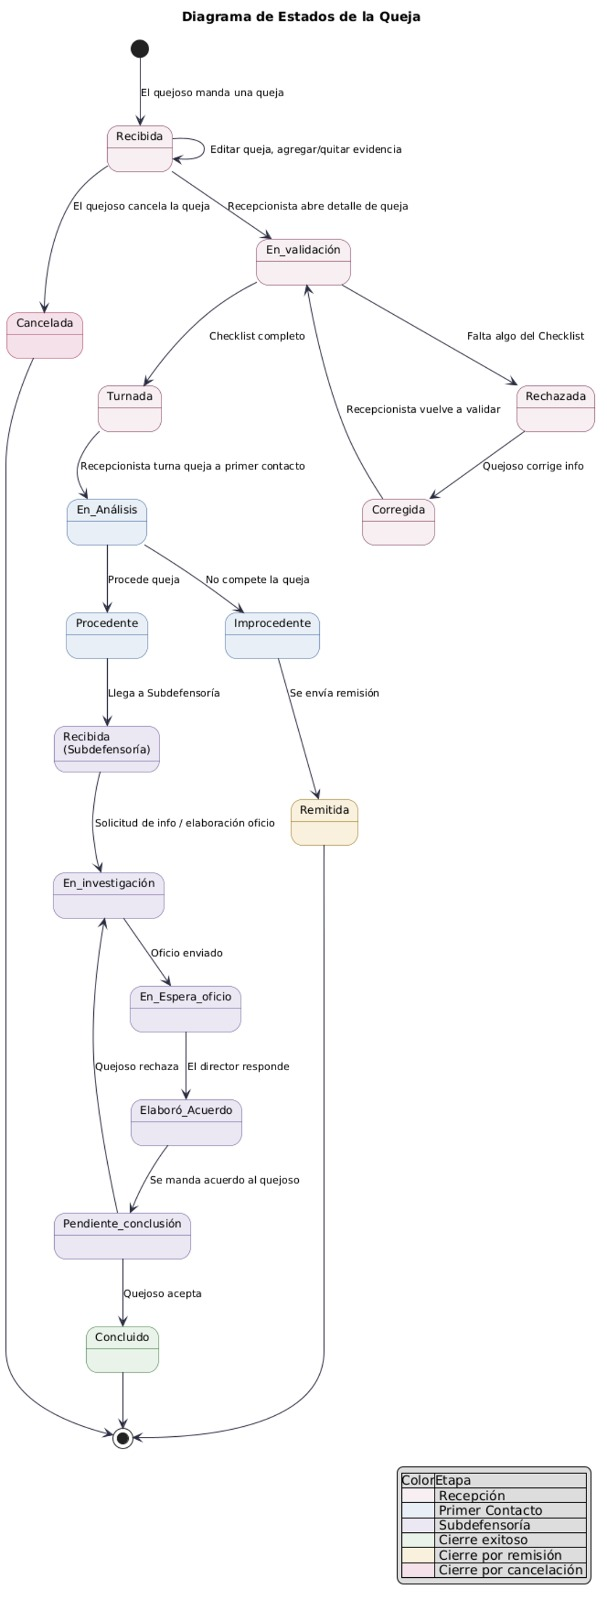
\includegraphics[height=0.82\textheight,keepaspectratio]{images/diagrama_estados_queja.png}
		\caption{Diagrama de estados de la queja}
		\label{fig:estados_queja}
	\end{figure}

	\rowcolors{2}{rowblue}{white}
	\small
	\renewcommand{\arraystretch}{1.2}
	\setlength{\tabcolsep}{4pt}
	\begin{longtable}{|p{4.4cm}|L{2.6cm}|L{3.3cm}|L{4.3cm}|}
		\caption{Estados y transiciones de la queja}
		\label{tab:estados} \\
		\hline
		\rowcolor{headerblue}
		\headercell{Estado} & \headercell{Área} & \headercell{Evento} & \headercell{Siguiente estado} \\
		\hline
		\endfirsthead
		\hline
		\rowcolor{headerblue}
		\headercell{Estado} & \headercell{Área} & \headercell{Evento} & \headercell{Siguiente estado} \\
		\hline
		\endhead
		(inicio) & Quejoso & Registra la queja & \texttt{RECIBIDA} \\ \hline
		\texttt{RECIBIDA} & Recepción & Una recepcionista la toma & \texttt{EN\_VALIDACION} \\ \hline
		\texttt{RECIBIDA} & Quejoso & Cancela & \texttt{CANCELADA} (final) \\ \hline
		\texttt{EN\_VALIDACION} & Recepción & Suelta la queja o vence la toma & \texttt{RECIBIDA} o
		\texttt{CORREGIDA} \\ \hline
		\texttt{EN\_VALIDACION} & Recepción & Regresa con observaciones & \texttt{RECHAZADA} \\ \hline
		\texttt{EN\_VALIDACION} & Recepción & Turna & \texttt{TURNADA} \\ \hline
		\texttt{RECHAZADA} & Quejoso & Corrige y reenvía & \texttt{CORREGIDA} \\ \hline
		\texttt{CORREGIDA} & Recepción & Una recepcionista la toma & \texttt{EN\_VALIDACION} \\ \hline
		\texttt{TURNADA} & Primer Contacto & El analista abre el expediente & \texttt{EN\_ANALISIS} \\ \hline
		\texttt{EN\_ANALISIS} & Primer Contacto & Dictamen de competencia & \texttt{PROCEDENTE} \\ \hline
		\texttt{EN\_ANALISIS} & Primer Contacto & Dictamen de improcedencia & \texttt{IMPROCEDENTE} \\ \hline
		\texttt{IMPROCEDENTE} & Primer Contacto & Envía la remisión & \texttt{REMITIDA} (final) \\ \hline
		\texttt{PROCEDENTE} & Subdefensoría & Recibe el expediente & \texttt{RECIBIDO} \\ \hline
		\texttt{RECIBIDO} & Subdefensoría & El subdefensor abre el expediente & \texttt{EN\_INVESTIGACION} \\ \hline
		\texttt{EN\_INVESTIGACION} & Subdefensoría & Envía la solicitud de información &
		\texttt{EN\_ESPERA\_OFICIO} \\ \hline
		\texttt{EN\_ESPERA\_OFICIO} & Subdefensoría & Registra la respuesta de la unidad &
		\texttt{ELABORO\_ACUERDO} \\ \hline
		\texttt{ELABORO\_ACUERDO} & Subdefensoría & Envía el acuerdo de conciliación &
		\texttt{PENDIENTE\_CONCILIACION} \\ \hline
		\texttt{PENDIENTE\_CONCILIACION} & Quejoso & Acepta el acuerdo & \texttt{PENDIENTE\_CONCLUSION} \\ \hline
		\texttt{PENDIENTE\_CONCILIACION} & Quejoso & Rechaza el acuerdo & \texttt{EN\_INVESTIGACION} \\ \hline
		\texttt{PENDIENTE\_CONCLUSION} & Subdefensoría & Envía el acuerdo de conclusión & \texttt{CONCLUIDO}
		(final) \\ \hline
	\end{longtable}
	\normalsize

	Dos decisiones del modelo merecen explicación. La primera es que tener una cita o notas no es un
	estado: son indicadores del expediente que no bloquean ninguna transición, porque en una versión
	temprana el pseudoestado ``con cita'' impedía dictaminar mientras hubiera una cita pendiente. La
	segunda es que \texttt{IMPROCEDENTE} no es final: toda queja improcedente concluye con la remisión a
	la autoridad competente, lo que garantiza que el quejoso reciba siempre una orientación sobre a dónde
	acudir.

	\subsection{Diseño de la arquitectura}
	\label{sec:diseno_arquitectura}
	La arquitectura se diseñó como un conjunto de microservicios organizados por capacidad del negocio:
	cada área de la Defensoría y cada función transversal tiene su propio servicio, su propia interfaz
	de programación y su propio contenedor. Esta sección presenta la vista de componentes, la vista de
	despliegue, la comunicación entre servicios y el diseño de la seguridad.

	\subsubsection{Vista de componentes}
	La Tabla~\ref{tab:microservicios} lista los servicios del lado del servidor con el puerto en que se
	publican, su responsabilidad y las tablas de las que son dueños. Todos los servicios Java siguen la
	misma estructura interna en capas (Sección~\ref{sec:impl_backend}) y escuchan dentro de su
	contenedor en el puerto 8080; el puerto de la tabla es el que se publica en el servidor de
	aplicación.

	\rowcolors{2}{rowblue}{white}
	\small
	\renewcommand{\arraystretch}{1.2}
	\setlength{\tabcolsep}{4pt}
	\begin{longtable}{|p{4.2cm}|p{1.0cm}|L{4.9cm}|L{4.4cm}|}
		\caption{Servicios del lado del servidor}
		\label{tab:microservicios} \\
		\hline
		\rowcolor{headerblue}
		\headercell{Servicio} & \headercell{Puerto} & \headercell{Responsabilidad} &
		\headercell{Tablas de las que es dueño} \\
		\hline
		\endfirsthead
		\hline
		\rowcolor{headerblue}
		\headercell{Servicio} & \headercell{Puerto} & \headercell{Responsabilidad} &
		\headercell{Tablas de las que es dueño} \\
		\hline
		\endhead
		\texttt{auth-\allowbreak{}service} & 8083 & Sesión del quejoso: inicio de sesión, activación, recuperación de
		contraseña y perfil. Emite el token del quejoso. & \texttt{usuarios} \\ \hline
		\texttt{quejas-\allowbreak{}service} & 8084 & Registro, consulta, edición, corrección y cancelación de quejas;
		evidencias; acuerdos del lado del quejoso. & \texttt{quejas}, \texttt{queja\_\allowbreak{}tutores},
		\texttt{queja\_\allowbreak{}evidencias} \\ \hline
		\texttt{notificaciones-\allowbreak{}service} & 8085 & Envío de correo por SMTP y centro de notificaciones de
		quejosos y personal. & \texttt{notificaciones} \\ \hline
		\texttt{catalogo-\allowbreak{}service} & 8086 & Catálogo de dependencias y unidades académicas del IPN. &
		\texttt{dependencias} \\ \hline
		\texttt{admin-\allowbreak{}service} & 8087 & Sesión del personal, cuentas, plantillas, respaldos, bitácora y
		paneles de seguimiento de la Defensora. Emite el token del personal. &
		\texttt{personal\_\allowbreak{}administrativo}, \texttt{plantillas\_\allowbreak{}documentos}, \texttt{bitacora\_\allowbreak{}acciones} \\ \hline
		\texttt{revision-\allowbreak{}service} & 8088 & Bandeja, toma, validación, regreso, turnado, ventanilla e
		historial de Recepción; acuerdos del lado del personal. & Columnas de flujo de \texttt{quejas};
		\texttt{acuerdos\_\allowbreak{}conciliacion} \\ \hline
		\texttt{chatbot-\allowbreak{}service} & 8089 & Preguntas frecuentes del portal y su administración. &
		\texttt{preguntas\_\allowbreak{}chatbot} \\ \hline
		\texttt{primer-contacto-\allowbreak{}service} & 8082 & Expedientes de análisis, citas, oficios, solicitudes a la
		persona señalada, dictámenes y remisiones. & \texttt{expedientes\_\allowbreak{}primer\_\allowbreak{}contacto},
		\texttt{citas\_\allowbreak{}primer\_\allowbreak{}contacto}, \texttt{notas\_\allowbreak{}analisis}, \texttt{dictamenes\_\allowbreak{}primer\_\allowbreak{}contacto},
		\texttt{remisiones\_\allowbreak{}externas}, \texttt{evidencias\_\allowbreak{}primer\_\allowbreak{}contacto}, \texttt{solicitudes\_\allowbreak{}denunciado} \\ \hline
		\texttt{subdefensoria-\allowbreak{}service} & 8091 & Expedientes de investigación, oficios, recordatorios,
		respuestas, control de plazos, alertas y acuerdos de conclusión. & \texttt{expedientes\_\allowbreak{}investigacion},
		\texttt{oficios\_\allowbreak{}informacion}, \texttt{recordatorios\_\allowbreak{}urgencia}, \texttt{respuestas\_\allowbreak{}externas},
		\texttt{respuestas\_\allowbreak{}externas\_\allowbreak{}archivos}, \texttt{acuerdos\_\allowbreak{}conclusion} \\ \hline
		\texttt{denunciado-\allowbreak{}service} & 8094 & Registro y consulta de la versión de la persona señalada. &
		\texttt{respuestas\_\allowbreak{}denunciado}, \texttt{respuesta\_\allowbreak{}denunciado\_\allowbreak{}archivos} \\ \hline
	\end{longtable}
	\normalsize

	Del lado del cliente, las cinco aplicaciones Angular son proyectos independientes, cada uno con su
	propio enrutamiento, guardas, interceptores y contenedor de publicación: el portal del quejoso
	(\texttt{/}), Recepción (\texttt{/revision/}), Primer Contacto (\texttt{/primer-contacto/}),
	Subdefensoría (\texttt{/subdefensoria/}) y el panel de la Defensora (\texttt{/admin/}).

	\subsubsection{Vista de despliegue}
	La plataforma se despliega en tres servidores virtuales privados con funciones separadas, de modo
	que cada uno exponga solo lo indispensable:

	\begin{itemize}
		\item \textbf{Servidor de publicación.} Ejecuta el proxy inverso público (puertos 80 y 443), que
		termina TLS, y los cinco contenedores Nginx que sirven las aplicaciones compiladas. Es el único
		servidor con puertos de aplicación abiertos a Internet.
		\item \textbf{Servidor de aplicación.} Ejecuta los diez microservicios Java. Sus puertos solo aceptan conexiones que llegan por la interfaz pública desde el servidor
		de publicación; las llamadas entre servicios del mismo servidor no se filtran.
		\item \textbf{Servidor de datos.} Ejecuta PostgreSQL~16. El puerto de la base solo acepta
		conexiones del servidor de aplicación y los respaldos diarios se guardan en el propio servidor.
	\end{itemize}

	El proxy enruta por prefijo de ruta, como muestra la Tabla~\ref{tab:enrutamiento}. Además de enrutar,
	bloquea con una respuesta 403 las rutas de uso exclusivo entre servicios, que no deben ser
	alcanzables desde Internet aunque el servicio de destino las declare públicas.

	\rowcolors{2}{rowblue}{white}
	\small
	\renewcommand{\arraystretch}{1.2}
	\setlength{\tabcolsep}{4pt}
	\begin{longtable}{|p{5.6cm}|p{4.6cm}|p{4.3cm}|}
		\caption{Enrutamiento del proxy inverso público}
		\label{tab:enrutamiento} \\
		\hline
		\rowcolor{headerblue}
		\headercell{Ruta pública} & \headercell{Destino} & \headercell{Observación} \\
		\hline
		\endfirsthead
		\hline
		\rowcolor{headerblue}
		\headercell{Ruta pública} & \headercell{Destino} & \headercell{Observación} \\
		\hline
		\endhead
		\texttt{/} & Portal del quejoso & Aplicación Angular \\ \hline
		\texttt{/revision/}, \texttt{/admin/}, \texttt{/primer-contacto/}, \texttt{/subdefensoria/} &
		Paneles del personal & Aplicaciones Angular \\ \hline
		\texttt{/api/auth/} & \texttt{auth-service} & \\ \hline
		\texttt{/api/quejoso/} & \texttt{quejas-service} & \\ \hline
		\texttt{/api/notificaciones/} & \texttt{notificaciones-service} & \texttt{/enviar} y
		\texttt{/registrar} bloqueadas \\ \hline
		\texttt{/api/catalogos/} & \texttt{catalogo-service} & \\ \hline
		\texttt{/api/admin/} & \texttt{admin-service} & \\ \hline
		\texttt{/api/revision/} & \texttt{revision-service} & \\ \hline
		\texttt{/api/chatbot/} & \texttt{chatbot-service} & \\ \hline
		\texttt{/api/denunciado/} & \texttt{denunciado-service} & \\ \hline
		\texttt{/api/primer-contacto/} & \texttt{primer-contacto-service} & \texttt{/ingesta/} bloqueada \\ \hline
		\texttt{/api/subdefensoria/} & \texttt{subdefensoria-service} & \texttt{/ingesta/} y
		\texttt{/acuerdos-conclusion/interno/} bloqueadas \\ \hline
	\end{longtable}
	\normalsize

	\subsubsection{Diseño de la comunicación entre servicios}
	La plataforma combina dos mecanismos de integración, elegidos según la naturaleza de cada relación.
	El primero es la \textbf{tabla compartida}: los servicios que necesitan conocer el estatus de una
	queja lo leen directamente de la tabla \texttt{quejas}, cada uno con su propia entidad de
	persistencia sobre ella, de modo que un cambio hecho por un área es visible de inmediato para las
	demás sin una llamada en línea. El segundo son las \textbf{llamadas REST síncronas}, que se usan
	cuando un servicio debe pedir a otro que haga algo. La Tabla~\ref{tab:comunicacion} enumera estas
	llamadas.

	\rowcolors{2}{rowblue}{white}
	\small
	\renewcommand{\arraystretch}{1.2}
	\setlength{\tabcolsep}{4pt}
	\begin{longtable}{|p{3.3cm}|p{3.3cm}|p{4.6cm}|p{3.3cm}|}
		\caption{Llamadas entre servicios}
		\label{tab:comunicacion} \\
		\hline
		\rowcolor{headerblue}
		\headercell{Origen} & \headercell{Destino} & \headercell{Propósito} & \headercell{Si falla} \\
		\hline
		\endfirsthead
		\hline
		\rowcolor{headerblue}
		\headercell{Origen} & \headercell{Destino} & \headercell{Propósito} & \headercell{Si falla} \\
		\hline
		\endhead
		\texttt{auth-service} & \texttt{quejas-service} & Validar el par folio--correo al activar una cuenta
		(cliente declarativo) & La activación se rechaza \\ \hline
		\texttt{quejas-service}, \texttt{revision-service}, \texttt{primer-contacto-service},
		\texttt{subdefensoria-service} & \texttt{notificaciones-service} & Enviar correos y registrar
		notificaciones & Se registra el error; la operación continúa \\ \hline
		\texttt{revision-service} & \texttt{primer-contacto-service} & Crear el expediente al turnar &
		El turnado se reporta como fallido y puede repetirse \\ \hline
		\texttt{primer-contacto-service} & \texttt{subdefensoria-service} & Crear el expediente de
		investigación al dictaminar competencia & El dictamen se conserva; se ofrece reenviar \\ \hline
		\texttt{primer-contacto-service} & \texttt{revision-service} & Obtener el contenido de una
		evidencia sin duplicar archivos & Se informa al usuario \\ \hline
	\end{longtable}
	\normalsize

	Todas las llamadas síncronas se configuraron con tiempos de espera explícitos ---tres segundos para
	conectar y diez para responder en los clientes de plantilla--- y las que corresponden a operaciones
	secundarias se ejecutan en modo de mejor esfuerzo. La consecuencia de diseño es que el fallo de un
	servicio auxiliar nunca deja colgada una petición del usuario ni revierte una operación principal ya
	guardada, conforme a los requerimientos RNF-Q04 y RNF-R04.

	\subsubsection{Diseño de la seguridad y el control de acceso}
	La seguridad se diseñó en capas, de modo que ningún mecanismo sea el único que protege un recurso:

	\begin{enumerate}
		\item \textbf{Red.} Solo el servidor de publicación acepta tráfico de Internet; el de aplicación y
		el de datos filtran por origen, con reglas aplicadas antes de las que inserta el motor de
		contenedores.
		\item \textbf{Proxy.} Termina TLS, redirige HTTP a HTTPS y bloquea las rutas internas.
		\item \textbf{Autenticación.} Dos emisores de tokens: \texttt{auth-service} para quejosos y
		\texttt{admin-service} para el personal. Ambos firman con HS256 y una vigencia de una hora; el
		token del personal incluye el rol. Cada microservicio valida el token de forma local con un filtro
		propio.
		\item \textbf{Autorización por rol.} Cada controlador declara los roles que admite, tanto por ruta
		en la cadena de filtros como por método con anotaciones.
		\item \textbf{Autorización por pertenencia.} Las consultas del quejoso se filtran por el correo del
		token; las de las recepcionistas, por la asignación de la queja; y la edición de oficios, por su
		autor.
		\item \textbf{Validación en el servidor.} Todas las reglas de negocio se verifican en el servicio,
		incluida la firma binaria de los archivos, y no solo en el formulario.
	\end{enumerate}

	La Tabla~\ref{tab:matriz_roles} resume qué rol puede usar cada grupo de puntos de acceso.

	\rowcolors{2}{rowblue}{white}
	\small
	\renewcommand{\arraystretch}{1.2}
	\setlength{\tabcolsep}{4pt}
	\begin{longtable}{|p{6.6cm}|p{7.9cm}|}
		\caption{Matriz de autorización por grupo de puntos de acceso}
		\label{tab:matriz_roles} \\
		\hline
		\rowcolor{headerblue}
		\headercell{Grupo de puntos de acceso} & \headercell{Acceso} \\
		\hline
		\endfirsthead
		\hline
		\rowcolor{headerblue}
		\headercell{Grupo de puntos de acceso} & \headercell{Acceso} \\
		\hline
		\endhead
		Inicio de sesión, activación y recuperación; registro público de quejas; consulta por folio;
		catálogo; menú del chatbot; respuesta de la persona señalada; respuesta a citas y acuerdos por
		enlace & Público (el enlace lleva un token de un solo propósito) \\ \hline
		Mis quejas, evidencias propias, corrección, cancelación, acuerdos y citas del quejoso & Token de
		quejoso; filtrado por el correo del token \\ \hline
		Notificaciones propias & Cualquier token válido \\ \hline
		\texttt{/api/revision/**} & \texttt{RECEPCIONISTA} \\ \hline
		Acuerdos de conciliación del personal & \texttt{RECEPCIONISTA}, \texttt{SUBDEFENSOR},
		\texttt{DEFENSOR} \\ \hline
		\texttt{/api/primer-contacto/**} & \texttt{ANALISTA\_PRIMER\_CONTACTO} \\ \hline
		Consulta de lo actuado en Primer Contacto, PDF de oficios y evidencias de Primer Contacto &
		\texttt{ANALISTA\_PRIMER\_CONTACTO}, \texttt{SUBDEFENSOR}, \texttt{DEFENSOR} \\ \hline
		\texttt{/api/subdefensoria/**} & \texttt{SUBDEFENSOR} \\ \hline
		Consulta de respuestas de la persona señalada & Todos los roles de personal \\ \hline
		Personal, plantillas, respaldos, bitácora, seguimiento, administración del catálogo y del chatbot &
		\texttt{DEFENSOR} \\ \hline
		Cambio de contraseña propia del personal & Cualquier rol de personal \\ \hline
		Envío de correo, registro de notificaciones e ingesta de expedientes & Solo entre servicios;
		bloqueado en el proxy \\ \hline
	\end{longtable}
	\normalsize

	\subsection{Diseño de la base de datos}
	\label{sec:diseno_bd}
	La base de datos \texttt{defensoria\_db} reúne las tablas de todos los servicios. El esquema lo
	genera Hibernate a partir de las entidades de cada servicio al arrancar, y los datos de referencia
	---dependencias, preguntas frecuentes y cuentas iniciales del personal--- se cargan con guiones
	idempotentes posteriores. La Tabla~\ref{tab:esquema_bd} agrupa las tablas por dominio.

	\rowcolors{2}{rowblue}{white}
	\small
	\renewcommand{\arraystretch}{1.2}
	\setlength{\tabcolsep}{4pt}
	\begin{longtable}{|p{2.8cm}|p{5.6cm}|p{6.1cm}|}
		\caption{Tablas de la base de datos por dominio}
		\label{tab:esquema_bd} \\
		\hline
		\rowcolor{headerblue}
		\headercell{Dominio} & \headercell{Tablas} & \headercell{Contenido principal} \\
		\hline
		\endfirsthead
		\hline
		\rowcolor{headerblue}
		\headercell{Dominio} & \headercell{Tablas} & \headercell{Contenido principal} \\
		\hline
		\endhead
		Quejosos & \texttt{usuarios} & Cuenta, contraseña cifrada, perfil y código de recuperación
		cifrado con su vigencia e intentos \\ \hline
		Quejas & \texttt{quejas}, \texttt{queja\_tutores}, \texttt{queja\_evidencias} & Datos de la queja,
		estatus, columnas del flujo de Recepción (asignación, validación, turnado, ventanilla), tutor y
		archivos binarios \\ \hline
		Persona señalada & \texttt{respuestas\_denunciado}, \texttt{respuesta\_denunciado\_archivos} &
		Versión de los hechos, aviso de privacidad aceptado y archivos \\ \hline
		Primer Contacto & \texttt{expedientes\_primer\_contacto}, \texttt{citas\_primer\_contacto},
		\texttt{notas\_analisis}, \texttt{dictamenes\_primer\_contacto}, \texttt{remisiones\_externas},
		\texttt{evidencias\_primer\_contacto}, \texttt{solicitudes\_denunciado} & Expediente de análisis,
		citas con categoría y modalidad, oficios, dictamen, remisión y referencias a evidencias \\ \hline
		Subdefensoría & \texttt{expedientes\_investigacion}, \texttt{oficios\_informacion},
		\texttt{recordatorios\_urgencia}, \texttt{respuestas\_externas},
		\texttt{respuestas\_externas\_archivos}, \texttt{acuerdos\_conclusion} & Expediente de
		investigación, oficios con fecha límite y estatus, recordatorios, respuestas y acuerdos \\ \hline
		Conciliación & \texttt{acuerdos\_conciliacion} & Acuerdo, destinatario, estado y respuesta \\ \hline
		Personal y auditoría & \texttt{personal\_administrativo}, \texttt{bitacora\_acciones} & Cuentas
		con rol, contraseña temporal y último acceso; acciones con usuario, IP y fecha \\ \hline
		Referencia & \texttt{dependencias}, \texttt{plantillas\_documentos}, \texttt{preguntas\_chatbot} &
		Catálogo institucional, plantillas y preguntas frecuentes \\ \hline
		Avisos & \texttt{notificaciones} & Notificación por destinatario, tipo, enlace y lectura \\ \hline
	\end{longtable}
	\normalsize


%% Implementacion y evaluacion del prototipo
	\section{Implementación}
	\label{cap:implementacion}
	Este capítulo documenta cómo se construyó la plataforma diseñada en el
	Capítulo~\ref{cap:analisis_diseno}: las herramientas empleadas, la estructura común de los
	microservicios y de las aplicaciones web, los mecanismos que hacen cumplir las reglas de negocio y
	los requerimientos no funcionales, la integración de los componentes de inteligencia artificial y el
	empaquetado y despliegue en los tres servidores. Cierra con los incidentes de operación que obligaron
	a corregir el diseño y con el estado de avance de cada componente. La verificación sistemática del
	sistema se presenta por separado en el Capítulo~\ref{cap:pruebas}.

	\subsection{Entorno de desarrollo y herramientas}
	\label{sec:entorno_herramientas}
	La Tabla~\ref{tab:herramientas} reúne las herramientas y bibliotecas con las que se construyó y opera
	la plataforma. Las versiones son las que se encuentran en los archivos de proyecto al cierre del
	Trabajo Terminal.

	\rowcolors{2}{rowblue}{white}
	\small
	\renewcommand{\arraystretch}{1.2}
	\setlength{\tabcolsep}{4pt}
	\begin{longtable}{|p{4.0cm}|L{2.6cm}|L{7.9cm}|}
		\caption{Herramientas y bibliotecas empleadas}
		\label{tab:herramientas} \\
		\hline
		\rowcolor{headerblue}
		\headercell{Herramienta} & \headercell{Versión} & \headercell{Uso en el proyecto} \\
		\hline
		\endfirsthead
		\hline
		\rowcolor{headerblue}
		\headercell{Herramienta} & \headercell{Versión} & \headercell{Uso en el proyecto} \\
		\hline
		\endhead
		Java (OpenJDK) & 21 & Lenguaje de los once microservicios \\ \hline
		Spring Boot & 3.5.16 / 3.3.5 & Marco de los microservicios (3.3.5 en Primer Contacto y
		Subdefensoría) \\ \hline
		Spring Security, Spring Data JPA, Hibernate & Las de Spring Boot & Autenticación, autorización y
		persistencia \\ \hline
		Spring Cloud OpenFeign & --- & Cliente declarativo de \texttt{auth-service} hacia
		\texttt{quejas-service} \\ \hline
		springdoc-openapi & 2.8.5 / 2.6.0 & Contrato OpenAPI e interfaz Swagger de cada servicio \\ \hline
		Lombok & --- & Generación de métodos de acceso en parte de los servicios \\ \hline
		OpenPDF & --- & Oficios de Primer Contacto y Subdefensoría en PDF \\ \hline
		Apache POI & --- & Exportación a \texttt{.xlsx} e importación del catálogo desde Excel \\ \hline
		OWASP Java Encoder & 1.3.1 & Neutralización de saltos de línea en los encabezados de correo \\ \hline
		Apache Maven & 3.9 & Construcción, pruebas y empaquetado \\ \hline
		Angular y Angular CLI & 21.2 & Las cinco aplicaciones web \\ \hline
		TypeScript & 5.9 & Lenguaje de las aplicaciones web \\ \hline
		Node.js & 22 & Compilación de las aplicaciones web \\ \hline
		Python y FastAPI & 3.11 & Servicio de resúmenes \\ \hline
		PostgreSQL & 16 & Base de datos \\ \hline
		Podman & --- & Motor de contenedores en los tres servidores \\ \hline
		Nginx & imagen \texttt{alpine} & Proxy inverso público y servidores de las aplicaciones \\ \hline
		Certbot / Let's Encrypt & --- & Certificado TLS y su renovación automática \\ \hline
		JUnit 5, Mockito, AssertJ & Las de Spring Boot & Pruebas unitarias \\ \hline
		JaCoCo & 0.8.12 & Cobertura de las pruebas \\ \hline
		Checkstyle & 10.21 & Verificación de la guía de estilo \\ \hline
		Git, GitHub y GitHub Actions & --- & Control de versiones y flujo de pruebas \\ \hline
	\end{longtable}
	\normalsize

	\subsection{Implementación del lado del servidor}
	\label{sec:impl_backend}
	Los once microservicios Java comparten una misma organización, de modo que quien conoce uno puede
	orientarse en cualquier otro. Esta sección describe esa estructura y los mecanismos transversales
	que la complementan.

	\subsubsection{Estructura común de un microservicio}
	Cada servicio es un proyecto Maven independiente con su propio archivo \texttt{pom.xml} y un nombre de
	artefacto fijo ---por ejemplo \texttt{quejas-service.jar}---, que es el que esperan los guiones de
	despliegue. Su código se organiza en los paquetes de la arquitectura en capas
	(Sección~\ref{sec:arquitectura_software}):

	\begin{itemize}
		\item \texttt{controller}: controladores REST, sin lógica de negocio; reciben DTO y delegan.
		\item \texttt{service}: reglas del dominio, transacciones y llamadas a otros servicios.
		\item \texttt{validacion}: en los servicios con formularios públicos, las reglas de captura
		concentradas en clases sin dependencias de Spring.
		\item \texttt{repository} y \texttt{entity}: repositorios de Spring Data y entidades JPA.
		\item \texttt{dto}: objetos de entrada y salida de la API.
		\item \texttt{config} y \texttt{security}: cadena de filtros, filtro JWT, CORS, clientes HTTP y
		OpenAPI.
		\item \texttt{exception}: excepciones del dominio y su manejador global.
	\end{itemize}

	La configuración se lee de un archivo \texttt{application.yml} propio de cada servicio. En producción
	ese archivo no forma parte de la imagen: se monta desde una carpeta del servidor, de modo que cambiar
	una dirección, un tiempo de espera o un límite de tamaño solo requiere reiniciar el contenedor
	(RT-09).

	\subsubsection{Verificación de tokens y control de acceso}
	Los dos servicios que inician sesión ---\texttt{auth-service} para quejosos y \texttt{admin-service}
	para el personal--- emiten tokens JWT firmados con HS256 y una vigencia de 3\,600 segundos. El de
	personal incluye la afirmación \texttt{rol}. Todos los demás servicios contienen un filtro
	\texttt{JwtAuthenticationFilter} que se ejecuta antes de la autenticación de Spring: extrae el token
	del encabezado \texttt{Authorization}, verifica su firma y vigencia con la clave compartida y, si es
	válido, registra al usuario en el contexto de seguridad con la autoridad \texttt{ROLE\_}\textit{rol}. Una
	petición sin token o con un token alterado o vencido continúa como anónima y es rechazada por la regla
	que corresponda.

	La autorización se declara en dos niveles. En la cadena de filtros de cada servicio se listan las
	rutas públicas y las protegidas; el orden importa, porque Spring aplica la primera regla que
	coincide, de modo que las rutas de administración ---por ejemplo,
	\texttt{/api/catalogos/dependencias/admin/**}--- se declaran antes que la regla pública general del
	mismo prefijo. En los controladores, la anotación \texttt{@PreAuthorize} fija los roles de cada
	método, lo que hace que la regla sea visible junto al código que protege y que pueda verificarse de
	forma estática (Capítulo~\ref{cap:pruebas}). Las peticiones de verificación previa con el método
	\texttt{OPTIONS} se permiten siempre, para que el navegador pueda completar el protocolo CORS.

	La pertenencia se verifica en la capa de servicios con la identidad del token. Todas las consultas
	del quejoso sobre ``sus'' recursos reciben el correo del token como parámetro y buscan por folio
	\emph{y} correo, de modo que cambiar el folio en la URL devuelve un error de recurso no encontrado
	en lugar de la queja de otra persona.

	\subsubsection{Validación de las reglas de captura}
	Las reglas del formulario de queja se implementaron en el paquete \texttt{validacion} de
	\texttt{quejas-service}, separado de los controladores y de la persistencia:

	\begin{itemize}
		\item \texttt{ReglasQueja} concentra las constantes normativas: expresión regular de nombres,
		longitudes, número de identificación de hasta diez dígitos, longitud mínima de la narración, tamaños
		máximos de archivos, número de imágenes de identificación y versión del aviso de privacidad. La
		aplicación del quejoso tiene una copia de estas reglas para validar antes de enviar, pero la
		autoridad es siempre la del servidor.
		\item \texttt{ValidadorCorreo} valida el formato general del correo y, en un segundo nivel, las
		reglas propias del proveedor más común, para detectar errores de captura.
		\item \texttt{ValidadorFechas} calcula la edad y la vigencia de las fechas en la zona horaria
		\texttt{America/Mexico\_City}, para que una queja registrada de noche no cambie de día.
		\item \texttt{DetectorTipoArchivo} lee los primeros doce bytes de cada archivo y determina su tipo
		real por la firma binaria (los ``números mágicos'' de PDF, JPEG, PNG, MP4 y MP3); un ejecutable
		renombrado con extensión \texttt{.jpg} se rechaza aunque el navegador declare un tipo de imagen
		(RNF-G08).
		\item \texttt{ValidadorQuejaPublica} aplica todas las anteriores y lanza una
		\texttt{ValidacionException} con un mensaje para el usuario ante la primera regla incumplida.
	\end{itemize}

	El servicio de la persona señalada reproduce las mismas reglas con su propio conjunto de constantes,
	y Recepción calcula el plazo de 90 días naturales con una constante única en su aplicación.

	\subsubsection{Coordinación entre recepcionistas}
	El requerimiento RNF-R06 ---una queja solo puede estar en atención por una recepcionista--- se
	implementó sin bloqueos en memoria ni tablas auxiliares. Al abrir una queja, \texttt{revision-service}
	ejecuta una única sentencia de actualización que asigna la queja a la recepcionista \emph{solo si} su
	estatus sigue siendo \texttt{RECIBIDA} o \texttt{CORREGIDA}. La base de datos ejecuta esa sentencia de
	forma atómica: si dos recepcionistas abren la misma queja en el mismo instante, una actualiza la fila
	y la otra recibe cero filas afectadas, y el sistema le informa que la queja ya está en atención. Se
	guarda además el estatus previo, para devolverla a él si se suelta.

	Las operaciones de regreso y turnado verifican primero que la queja pertenezca a quien las solicita.
	La aplicación renueva la asignación cada cuatro minutos mientras la queja está abierta y, si se
	abandona, el servicio la libera a los veinte minutos de inactividad. La bandeja dejó de descargar las
	quejas completas en cada actualización: la consulta es paginada y el indicador de documentación se
	calcula con un conteo, no cargando los archivos.

	\subsubsection{Integración y resiliencia entre servicios}
	Las llamadas entre servicios se implementaron con \texttt{RestTemplate} configurado con tiempos de
	espera de tres segundos para conectar y diez para responder, y con un cliente OpenFeign con tiempos
	equivalentes en \texttt{auth-service}. Las llamadas a \texttt{notificaciones-service} están
	envueltas en bloques que capturan cualquier error de red o de servidor, lo registran y continúan
	(RNF-Q04, RNF-R04): la queja ya se guardó antes de notificar, de modo que el fallo del correo solo se
	pierde como aviso.

	El paso de expedientes entre áreas se implementó con dos garantías adicionales. El turnado es
	idempotente: si Recepción repite la llamada por un error de red, Primer Contacto reconoce el folio y
	no crea un segundo expediente. Y el dictamen de competencia se guarda antes de llamar a
	Subdefensoría: si esta no responde, el expediente queda marcado como pendiente de envío y la
	interfaz ofrece reenviarlo.

	Cada área tiene un único punto donde cambia el estatus de sus expedientes, la clase
	\texttt{TransicionExpedienteService}, que además refleja el nuevo estatus en la columna
	\texttt{estatus} de la tabla \texttt{quejas}. Concentrar el cambio en una sola clase garantiza que no
	haya caminos que actualicen el expediente sin actualizar la queja, defecto que existió en una versión
	temprana y que hacía que Recepción, la Defensora y el quejoso no vieran el avance de las etapas
	posteriores.

	\subsubsection{Seguridad complementaria}
	Además de los tokens, los servicios implementan los siguientes mecanismos:

	\begin{itemize}
		\item Contraseñas con BCrypt en \texttt{usuarios} y \texttt{personal\_administrativo}, con la
		política de RN-Q07.
		\item Código de recuperación de seis dígitos guardado cifrado, con vigencia de diez minutos y un
		máximo de cinco intentos; al agotarse, el código se invalida.
		\item Cuentas de personal creadas o restablecidas con contraseña temporal y cambio obligatorio, y
		una cuenta técnica inicial autoprovisionada en el primer arranque (RNF-A01).
		\item Protección contra quedarse sin administración: \texttt{PersonalAdministrativoService} impide
		desactivar o quitar el rol a la propia cuenta y a la última cuenta activa de administración
		(RNF-A07).
		\item Bitácora con la IP real del cliente, tomada de los encabezados \texttt{X-Real-IP} y
		\texttt{X-Forwarded-For} que añade el proxy, e inicios de sesión fallidos (RNF-A02).
		\item Neutralización de saltos de línea en asunto y destinatario de los correos, para impedir la
		inyección de encabezados (CWE-93).
		\item Enlaces de respuesta para citas y acuerdos con un token aleatorio de un solo propósito, que
		permite al quejoso responder sin iniciar sesión sin exponer otros datos.
	\end{itemize}

	\subsubsection{Manejo centralizado de errores y documentación}
	Los servicios cuentan con un manejador global (\texttt{@RestControllerAdvice}) que traduce las
	excepciones del dominio a respuestas HTTP con un cuerpo uniforme: las de validación a 400, las de
	acceso a 403, las de recurso no encontrado a 404, las de conflicto a 409, las peticiones que exceden
	el tamaño permitido a 413 y cualquier error no previsto a 500 sin exponer la traza. Así, la interfaz puede mostrar el mensaje del servidor sin interpretar trazas de error
	(RNF-Q07). En los ocho servicios desarrollados por el equipo, un filtro de registro escribe una línea por petición con método, ruta, estatus y duración,
	lo que permitió diagnosticar los incidentes de la Sección~\ref{sec:incidentes}.

	Los once servicios publican su contrato con springdoc-openapi en \texttt{/v3/api-docs} y una interfaz
	navegable en \texttt{/swagger-ui.html} (RNF-G03). Como los puertos de los servicios no son
	alcanzables desde Internet, la documentación se consulta mediante un túnel SSH desde el servidor de
	publicación.

	\subsubsection{Puntos de acceso implementados}
	La Tabla~\ref{tab:endpoints} resume, por servicio, el número de puntos de acceso y los grupos
	funcionales que cubren. El catálogo detallado, con el rol que exige cada uno, se genera de forma
	automática a partir del código y se usa como insumo de las pruebas de seguridad
	(Sección~\ref{sec:pruebas_seguridad}).

	\rowcolors{2}{rowblue}{white}
	\small
	\renewcommand{\arraystretch}{1.2}
	\setlength{\tabcolsep}{4pt}
	\begin{longtable}{|p{3.6cm}|L{1.4cm}|L{9.5cm}|}
		\caption{Puntos de acceso por servicio}
		\label{tab:endpoints} \\
		\hline
		\rowcolor{headerblue}
		\headercell{Servicio} & \headercell{Puntos} & \headercell{Grupos funcionales} \\
		\hline
		\endfirsthead
		\hline
		\rowcolor{headerblue}
		\headercell{Servicio} & \headercell{Puntos} & \headercell{Grupos funcionales} \\
		\hline
		\endhead
		\texttt{auth-service} & 7 & Inicio de sesión, activación, existencia de cuenta, código de
		recuperación, restablecimiento y perfil \\ \hline
		\texttt{quejas-service} & 15 & Registro público y con sesión, validación de folio, consulta por
		folio, mis quejas, edición, corrección, cancelación, evidencias y acuerdos \\ \hline
		\texttt{notificaciones-service} & 5 & Envío de correo y registro (internos), mis notificaciones, no
		leídas y marcado \\ \hline
		\texttt{catalogo-service} & 6 & Consulta pública y administración del catálogo, importación desde
		Excel \\ \hline
		\texttt{admin-service} & 32 & Inicio de sesión, personal, plantillas, respaldos, bitácora, tablero,
		seguimiento de quejas, unidades, carga y personal \\ \hline
		\texttt{revision-service} & 19 & Bandeja, toma, liberación, renovación, validación, regreso,
		turnado, abogados, antecedentes, ventanilla, historial, catálogos y acuerdos \\ \hline
		\texttt{chatbot-service} & 5 & Menú público y administración de preguntas \\ \hline
		\texttt{denunciado-service} & 3 & Registro público de la respuesta y consulta del personal \\ \hline
		\texttt{primer-contacto-service} & 56 & Bandeja, expedientes, citas (personal, quejoso y enlace
		público), oficios, solicitudes a la persona señalada, dictámenes, remisiones, conciliación,
		antecedentes, resumen, abogados, evidencias, consulta para Subdefensoría e ingesta \\ \hline
		\texttt{subdefensoria-service} & 30 & Bandeja, expedientes, oficios, recordatorios, respuestas y
		archivos, documentos PDF, control de plazos, alertas, acuerdos de conclusión, acuerdos por enlace e
		ingesta \\ \hline
		\texttt{antecedentes-service} & 6 & Búsqueda, resumen extractivo, corpus, entrenamiento y salud \\ \hline
		\textbf{Total} & \textbf{184} & \\ \hline
	\end{longtable}
	\normalsize

	\subsection{Implementación de las aplicaciones web}
	\label{sec:impl_frontend}
	Las cinco aplicaciones se construyeron con Angular~21 sin un repositorio común: cada una es un
	proyecto independiente con su propio \texttt{package.json}, su compilación y su contenedor. La
	independencia se aceptó a cambio de duplicar algunos archivos compartidos, que se mantienen como
	copias idénticas y se documentan como tales.

	\subsubsection{Estructura común}
	Todas las aplicaciones usan componentes independientes y se organizan en \texttt{core} (servicios
	HTTP, modelos, guardas, interceptores, sesión y reglas de validación), \texttt{shared} (componentes
	reutilizables) y \texttt{pages} o \texttt{features} (una carpeta por pantalla). Las rutas se declaran
	con carga diferida (\texttt{loadComponent}), de modo que cada pantalla se descarga la primera vez que
	se visita: en el portal del quejoso el paquete inicial bajó de unos 600~KB a 320~KB (90~KB
	comprimido), y en Primer Contacto de 1.19~MB a 361~KB. El asistente de preguntas frecuentes se carga
	con un bloque diferido cuando la página ya está inactiva.

	\subsubsection{Interceptores, guardas y sesión}
	Cada aplicación registra tres interceptores HTTP. El de autenticación añade el token a las peticiones
	dirigidas a la API. El de errores cierra la sesión y redirige al inicio de sesión ante una respuesta
	401 o 403 de un servicio de negocio (RNF-Q06), con excepción de las respuestas del servicio de
	notificaciones, cuyo fallo no debe expulsar al usuario. El tercero fuerza la detección de cambios al
	terminar cada petición, necesario porque las aplicaciones usan el modo sin zonas. Las guardas de ruta
	comprueban que exista una sesión vigente y, en los paneles del personal, que el rol corresponda al
	panel.

	El inicio de sesión del personal es único: la lógica compartida en \texttt{sesion-personal.ts} borra
	cualquier sesión previa al iniciar una nueva ---para que en una computadora compartida una
	recepcionista no herede la sesión de la Defensora---, redirige según el rol y cierra a la vez las
	sesiones de todos los paneles al salir.

	\subsubsection{Componentes compartidos}
	Entre los componentes reutilizables destacan el formulario de queja, que Recepción reutiliza para el
	registro en ventanilla; el autocompletado de dependencias sobre el catálogo; el selector de fechas; el
	aviso de privacidad; la campana de notificaciones de los paneles del personal, que se actualiza cada
	minuto; la ventana de programación de citas, usada tanto en la agenda como en el expediente; y, en el
	panel de la Defensora, un conjunto de componentes de tablero ---paginador, ventana modal, gráficas de
	dona y de barras, exportación a CSV y tablas de atención, unidades, carga y motivos---.

	\subsection{Integración de los componentes de inteligencia artificial}
	\label{sec:impl_ia}
	Los dos componentes de apoyo se integraron con Primer Contacto conforme al diseño de la
	Sección~\ref{sec:diseno_ia}:

	\begin{itemize}
		\item \texttt{antecedentes-service} es un servicio Spring Boot que expone
		\texttt{POST /api/antecedentes/buscar} con la narración y devuelve los antecedentes con su
		similitud, el fragmento relevante y los datos básicos de la queja. Primer Contacto filtra después
		los resultados que corresponden a la misma persona quejosa o señalada y muestra los cuatro más
		parecidos.
		\item \texttt{resumen-service} es un servicio Python con FastAPI que recibe la narración, selecciona
		los fragmentos de mayor relevancia y produce un borrador editado por un modelo de lenguaje ejecutado
		en un servidor de inferencia local. Devuelve el borrador y los fragmentos que lo sustentan.
	\end{itemize}

	Primer Contacto los invoca con un tiempo de espera configurable (110~s para el resumen, que es la
	operación más costosa). Si un componente no responde, la pestaña de análisis lo indica y muestra un
	resumen de respaldo generado en el navegador; el
	resto del expediente sigue operando.

	\subsection{Empaquetado en contenedores y despliegue}
	\label{sec:impl_despliegue}
	Cada componente se distribuye como una imagen de contenedor propia. Los microservicios Java usan un
	\texttt{Dockerfile} común que recibe el nombre del artefacto como argumento de construcción, salvo
	\texttt{admin-service}, que tiene uno propio porque necesita el cliente de PostgreSQL~16 para generar
	y restaurar respaldos. Las aplicaciones web se publican con una imagen de Nginx que sirve los archivos
	compilados. La Tabla~\ref{tab:contenedores} resume los contenedores por servidor.

	\rowcolors{2}{rowblue}{white}
	\small
	\renewcommand{\arraystretch}{1.2}
	\setlength{\tabcolsep}{4pt}
	\begin{longtable}{|p{2.5cm}|L{4.8cm}|L{3.0cm}|L{4.2cm}|}
		\caption{Contenedores por servidor}
		\label{tab:contenedores} \\
		\hline
		\rowcolor{headerblue}
		\headercell{Servidor} & \headercell{Contenedores} & \headercell{Puertos} &
		\headercell{Memoria} \\
		\hline
		\endfirsthead
		\hline
		\rowcolor{headerblue}
		\headercell{Servidor} & \headercell{Contenedores} & \headercell{Puertos} &
		\headercell{Memoria} \\
		\hline
		\endhead
		Publicación & \texttt{router-nginx} & 80, 443 (público) & --- \\ \hline
		Publicación & \texttt{defensoria-web}, \texttt{admin-web}, \texttt{revision-web},
		\texttt{primer-contacto-web}, \texttt{subdefensoria-web} & 8090, 8091, 8092, 8094, 8095 (locales) &
		--- \\ \hline
		Aplicación & \texttt{quejas-service} & 8084 & 1~GB, montón de 640~MB \\ \hline
		Aplicación & \texttt{auth-service}, \texttt{notificaciones-service}, \texttt{catalogo-service},
		\texttt{admin-service}, \texttt{revision-service}, \texttt{chatbot-service},
		\texttt{denunciado-service}, \texttt{primer-contacto-service}, \texttt{subdefensoria-service} &
		8083, 8085--8089, 8094, 8082, 8091 & 512~MB, montón de 320~MB \\ \hline
		Aplicación & \texttt{antecedentes-service}, \texttt{resumen-service} & 8093, 8090 & Según el modelo \\ \hline
		Datos & \texttt{defensoria-db} (PostgreSQL 16) & 5432 & --- \\ \hline
	\end{longtable}
	\normalsize

	Todos los contenedores se crean con la política de reinicio \texttt{always} y el servicio de reinicio
	de Podman habilitado, de modo que se levantan solos si terminan o si el servidor se reinicia
	(RNF-G04). Los servicios Java propios se ejecutan además con la opción
	\texttt{-XX:+ExitOnOutOfMemoryError}: si agotan la memoria, el registro muestra el error antes de que
	el contenedor se reinicie, en lugar de una terminación silenciosa por parte del núcleo.

	\subsubsection{Guiones de despliegue}
	El despliegue se automatizó con guiones de Bash, uno por servidor, en lugar de una plataforma de
	orquestación, conforme a la escala del proyecto (Sección~\ref{sec:tecnologias}):

	\begin{itemize}
		\item \texttt{podman-compose.sh} construye la imagen y crea el contenedor de cada microservicio con
		su puerto, memoria, variables y carpeta de configuración (\texttt{up}, \texttt{up-container},
		\texttt{delete}).
		\item \texttt{podman-compose-bd.sh} crea la base, aplica el cortafuegos de la base, carga los datos
		de referencia de forma idempotente y transaccional, y genera o restaura respaldos comprimidos. Un
		respaldo diario se programa a las 4:00 con \texttt{cron}.
		\item \texttt{firewall-backend.sh} restringe los puertos 8082 a 8094 a conexiones desde el servidor
		de publicación.
		\item Un guion por aplicación web reconstruye su contenedor a partir de la carpeta compilada.
	\end{itemize}

	Los cortafuegos se implementaron con reglas en la tabla \texttt{raw} de \texttt{iptables}, que se
	evalúa antes que las reglas de traducción que inserta Podman al publicar un puerto; una regla de
	\texttt{ufw} sobre el mismo puerto no habría tenido efecto (Sección~\ref{sec:tecnologias}). Las reglas
	se limitan a la interfaz pública del servidor, de modo que no afectan las llamadas entre contenedores.

	\subsubsection{Publicación segura y configuración del proxy}
	El proxy público redirige todo el tráfico HTTP a HTTPS con una respuesta 301, acepta solo TLS 1.2 y
	1.3 con el certificado de Let's Encrypt renovado por Certbot, y limita las peticiones a 100~MB. Además:

	\begin{itemize}
		\item Bloquea con 403 las rutas internas de notificaciones e ingesta
		(Tabla~\ref{tab:enrutamiento}).
		\item Comprime con \texttt{gzip} los archivos JavaScript, CSS y SVG, pero no las respuestas JSON de
		la API, para no exponerse a ataques de tipo BREACH.
		\item Sirve con caché de un año los archivos cuyo nombre incluye un resumen de su contenido, y sin
		caché el \texttt{index.html} y la API, de modo que cada despliegue se ve de inmediato.
		\item Reenvía a los servicios la IP real del cliente en los encabezados \texttt{X-Real-IP} y
		\texttt{X-Forwarded-For}.
	\end{itemize}

	\subsection{Incidentes de operación y correcciones}
	\label{sec:incidentes}
	La operación del sistema en los servidores reveló defectos que las pruebas de compilación no podían
	detectar. Se documentan porque cada uno originó un requerimiento o una prueba del
	Capítulo~\ref{cap:pruebas}.

	\paragraph{Peticiones colgadas al registrar una queja.} El formulario público mostraba un error,
	aunque la queja sí se guardaba. La causa era una regla de cortafuegos que descartaba sin responder
	todo el tráfico hacia los puertos de los servicios que no viniera del servidor de publicación,
	incluidas las llamadas del servicio de quejas al de notificaciones; como el cliente HTTP no tenía
	tiempo de espera, la petición esperaba hasta que el proxy la cortaba. La corrección limitó la regla a
	la interfaz pública y añadió tiempos de espera a todos los clientes HTTP.

	\paragraph{Terminación por memoria al recibir evidencias grandes.} Con seis archivos, uno de
	12.5~MB, el servicio de quejas terminaba sin mensaje de error y el navegador recibía un error 502. El
	núcleo lo detenía por exceder su límite de memoria, porque cada archivo se copia varias veces en
	memoria al guardarse como contenido binario. Se dimensionó el contenedor a 1~GB con un montón de
	640~MB, suficiente para una petición de 100~MB, y se añadió la terminación explícita por falta de
	memoria y el reinicio automático.

	\paragraph{Correo de observaciones que nunca se enviaba.} Recepción y el servicio de quejas invocaban
	un punto de envío de correo que no existía en el servicio de notificaciones; como la llamada era de
	mejor esfuerzo, el error solo quedaba en el registro y el quejoso nunca recibía las observaciones. Se
	implementó el punto de acceso con el contrato que ya usaban los clientes. El incidente mostró el
	límite de la degradación controlada: ocultar un fallo al usuario no debe ocultarlo también al equipo,
	y motivó la revisión de los registros como parte de las pruebas.

	\paragraph{Rutas internas expuestas a Internet.} Las rutas de envío de correo y registro de
	notificaciones eran públicas para que los servicios las invocaran sin token, y el proxy reenviaba
	todo el prefijo, de modo que cualquiera podía enviar correos desde la cuenta de la Defensoría. Se
	bloquearon en el proxy, y el mismo criterio se aplicó a las rutas de ingesta de Primer Contacto y
	Subdefensoría.

	\paragraph{Pérdida de datos en Primer Contacto y Subdefensoría.} Ambos servicios se desarrollaron
	inicialmente con una base en memoria, de modo que sus expedientes se perdían con cada reinicio y el
	personal no se encontraba en su copia de la tabla de cuentas. Se migraron a la base compartida.


	\subsection{Estado de avance por componente}
	\label{sec:estado_avance}
	La Tabla~\ref{tab:estado_avance} resume el estado de cada componente al cierre del proyecto, con las
	limitaciones conocidas que no impiden su operación.

	\rowcolors{2}{rowblue}{white}
	\small
	\renewcommand{\arraystretch}{1.2}
	\setlength{\tabcolsep}{4pt}
	\begin{longtable}{|p{3.5cm}|L{2.2cm}|L{8.8cm}|}
		\caption{Estado de avance por componente}
		\label{tab:estado_avance} \\
		\hline
		\rowcolor{headerblue}
		\headercell{Componente} & \headercell{Estado} & \headercell{Observaciones} \\
		\hline
		\endfirsthead
		\hline
		\rowcolor{headerblue}
		\headercell{Componente} & \headercell{Estado} & \headercell{Observaciones} \\
		\hline
		\endhead
		Portal del quejoso & Desplegado & El perfil valida el formato del teléfono pero no aplica todavía
		las mismas reglas del registro al correo personal y al domicilio (CU-QJ-05); la cancelación no
		registra el motivo (CU-QJ-15). \\ \hline
		Respuesta de la persona señalada & Desplegado & El folio llega en el enlace; falta un token que
		garantice que solo la persona señalada real responda. \\ \hline
		Panel de Recepción & Desplegado & El rango de fechas del historial filtra por la fecha de registro,
		no por la de atención; el visor de PDF del navegador permite descargar la evidencia que se
		visualiza (CU-REC-03). \\ \hline
		Panel de Primer Contacto & Desplegado & Todos los expedientes son visibles para todos los analistas;
		la asignación por analista está pendiente de acuerdo con la Defensoría. \\ \hline
		Panel de Subdefensoría & Desplegado & ``Mis expedientes'' muestra todos los expedientes hasta que se
		implemente la asignación por abogado. \\ \hline
		Panel de la Defensora & Desplegado & Completo según el documento de diseño. \\ \hline
		Componentes de IA & Desplegados & Su calidad depende del corpus disponible
		(Sección~\ref{sec:limitaciones}). \\ \hline
		Seguridad transversal & Con pendientes & Los secretos de configuración residen en texto plano en el
		repositorio; el proxy no envía HSTS; la descarga y restauración de respaldos no valida que el nombre
		de archivo permanezca dentro de la carpeta de respaldos; no existe cierre de sesión por inactividad
		en los paneles del personal. Se detallan en la Sección~\ref{sec:pruebas_seguridad}. \\ \hline
	\end{longtable}
	\normalsize


%% Modulos de la Plataforma
	\section{Módulos de la Plataforma}
	\label{cap:modulos}
	Este capítulo presenta el recorrido funcional de cada aplicación de la plataforma tal como la usa
	cada actor. Mientras el Capítulo~\ref{cap:analisis_diseno} describe qué debe hacer el sistema y el
	Capítulo~\ref{cap:implementacion} cómo se construyó, aquí se describe qué encuentra cada persona al
	entrar y cómo avanza una queja de un módulo al siguiente. Los módulos se presentan en el orden del
	procedimiento: el portal del quejoso, la respuesta de la persona señalada, Recepción, Primer
	Contacto, Subdefensoría y el panel de la Defensora. La última sección relaciona cada módulo con los
	casos de uso que implementa.

	\subsection{Portal del quejoso}
	\label{sec:modulo_quejoso}
	El portal se publica en la raíz del dominio y es la única aplicación dirigida al público. Tiene un
	área pública, que no requiere cuenta, y un panel autenticado para quien activa una cuenta de
	seguimiento.

	\subsubsection{Área pública}
	\begin{itemize}
		\item \textbf{Inicio.} Presenta la Defensoría, sus atribuciones y los accesos a presentar una queja,
		consultarla y entrar al panel. El asistente de preguntas frecuentes flota en todas las páginas y
		muestra las preguntas agrupadas por categoría (CU-QJ-06).
		\item \textbf{Presentar una queja} (\texttt{/queja/registro}). Formulario en pasos numerados:
		datos de la persona quejosa, datos de la unidad y de los hechos, persona señalada, narración y
		archivos. La unidad se elige con un autocompletado sobre el catálogo institucional; la fecha de
		nacimiento determina si se abre la sección del tutor; los archivos se previsualizan antes de
		enviar y cada campo muestra el mensaje de la regla que incumple. Al final se acepta el aviso de
		privacidad y se envía; el acuse muestra el folio y ofrece crear la cuenta de seguimiento
		(CU-QJ-07).
		\item \textbf{Consultar mi queja} (\texttt{/queja/consultar}). Con el folio y el correo muestra el
		estatus y el detalle de la queja (CU-QJ-11).
		\item \textbf{Crear o activar cuenta} (\texttt{/cuenta/crear}, \texttt{/cuenta/activar}). Solicita
		el folio, el correo y una contraseña que cumpla la política (CU-QJ-02).
		\item \textbf{Iniciar sesión y recuperar contraseña} (\texttt{/portal/login},
		\texttt{/portal/recuperar}). La recuperación se hace en dos pasos: solicitar el código y capturarlo
		con la nueva contraseña (CU-QJ-01, CU-QJ-03, CU-QJ-04).
		\item \textbf{Responder una cita o un acuerdo} (\texttt{/cita/responder},
		\texttt{/acuerdo/responder}). Páginas a las que llevan los enlaces enviados por correo: muestran la
		cita de Primer Contacto o el acuerdo de Subdefensoría y permiten confirmarla, cancelarla, aceptarlo
		o rechazarlo sin iniciar sesión (CU-QJ-14, CU-PC-04).
	\end{itemize}

	\subsubsection{Panel autenticado}
	El panel (\texttt{/panel}) tiene un menú lateral con las siguientes vistas:

	\begin{itemize}
		\item \textbf{Resumen.} Conteo de quejas propias por estatus.
		\item \textbf{Mis quejas.} Lista con filtros por estatus y texto. El detalle de cada queja muestra
		sus datos, sus evidencias ---que pueden verse o descargarse---, la línea de tiempo de estatus y, si
		Recepción la regresó, las observaciones. Mientras la queja está en \texttt{RECIBIDA}, el detalle
		permite editarla, agregar o quitar evidencias y cancelarla; si está \texttt{RECHAZADA}, permite
		corregirla y reenviarla (CU-QJ-08 a CU-QJ-10, CU-QJ-12, CU-QJ-15).
		\item \textbf{Nueva queja.} El mismo formulario del área pública sin la sección de identidad, que se
		toma de la sesión.
		\item \textbf{Conciliación.} Acuerdos dirigidos al quejoso con su asunto, términos y estado; los
		pendientes pueden aceptarse o rechazarse con un comentario (CU-QJ-13, CU-QJ-14).
		\item \textbf{Notificaciones.} Centro de avisos con el contador de no leídas que también se muestra
		en el menú (CU-NOT-01).
		\item \textbf{Perfil.} Datos de solo lectura de la cuenta y datos de contacto editables (CU-QJ-05).
	\end{itemize}

	\subsection{Respuesta de la persona señalada}
	\label{sec:modulo_denunciado}
	La página \texttt{/denunciado/respuesta} forma parte del portal pero está dirigida a la persona a
	quien se atribuyen los hechos. Muestra en la parte superior el folio de la queja a la que responde
	---recibido en el enlace---, y solicita su identidad, unidad de procedencia, tipo y número de
	identificación, su versión de los hechos, una o dos imágenes de su credencial y sus evidencias. Antes
	de enviar debe aceptar un aviso de privacidad propio, redactado para su situación. El acuse muestra el
	folio de respuesta \texttt{RD-XXXXXXXX} (RF-D01). El personal consulta las respuestas desde el
	expediente correspondiente.

	\subsection{Panel de Recepción}
	\label{sec:modulo_revision}
	El panel se publica en \texttt{/revision/} y su pantalla de inicio de sesión es la entrada única del
	personal: tras autenticarse, cada persona es dirigida al panel de su rol (CU-ADM-07).

	\subsubsection{Bandeja}
	La bandeja muestra en la parte superior los indicadores del día ---por atender, en atención, atendidas
	hoy, espera más larga, resaltada en ámbar desde los tres días, y tiempo de respuesta promedio de los
	últimos 30 días--- y debajo la cola paginada, con la queja más reciente primero, filtros por pestaña
	(todas, disponibles, mías, corregidas, en atención) y búsqueda. Cada fila indica el folio, la persona
	quejosa, la unidad, la antigüedad, si llegó por ventanilla y si otra recepcionista la está atendiendo.
	El recuadro ``Equipo de Recepción'' muestra la actividad de cada recepcionista en el día (CU-REC-01).

	\subsubsection{Validación de requisitos}
	Al abrir una queja, esta queda a nombre de quien la abrió (CU-REC-02) y se muestra la pantalla de
	validación. A la izquierda aparecen los datos de la queja y los documentos, que se abren en el
	navegador (CU-REC-03); a la derecha, la lista de verificación con los cinco requisitos de admisión,
	cada uno con su fundamento y su criterio de cotejo:

	\begin{enumerate}
		\item Identidad de la persona quejosa: nombre y apellidos completos, con la aclaración de que hay
		personas con un solo apellido.
		\item Documentación de identidad: se muestra el catálogo agrupado de documentos aceptados
		---identificación oficial, identificación institucional del IPN y documentos de representación---
		para elegir el que se exhibió.
		\item Matrícula institucional, en dos pasos: primero la boleta y, si no aplica, el número de
		empleado, ambos con la opción ``no aplica''.
		\item Oportunidad: el sistema muestra la fecha de los hechos, la de presentación y los días
		transcurridos, con la leyenda ``en término'' o ``término fenecido'' según el plazo de 90 días.
		\item Identificación de la persona señalada.
	\end{enumerate}

	Cada requisito se responde con ``sí'', ``no'' o, cuando corresponde, ``no aplica''; un ``no'' exige una
	observación. El botón ``Turnar'' solo se habilita con los cinco requisitos satisfechos; con al menos
	uno no satisfecho, el botón disponible es ``Regresar al quejoso'', que arma los motivos con la misma
	redacción de los requisitos y envía el correo (CU-REC-04). La recepcionista puede soltar la queja para
	que otra la atienda.

	\subsubsection{Turnado}
	La pantalla de turnado muestra los antecedentes de la queja como tarjetas ---folio, fecha, unidad,
	estado actual, abogado que la lleva y si se trata de la misma persona quejosa o de la misma persona
	señalada--- y la lista de abogados ordenada por su carga en trámite, con el sugerido preseleccionado.
	Si se elige a alguien con más carga, aparece un aviso. Al confirmar, la queja sale de la cola y se crea
	el expediente en Primer Contacto (CU-REC-05).

	\subsubsection{Registro en ventanilla e historial}
	El registro en ventanilla reutiliza el formulario del portal y agrega la sección ``Recepción en
	ventanilla'' con el documento recibido, la fecha de recepción física, el número de oficio y la
	ubicación del expediente; la queja aparece en la cola con la etiqueta ``Ventanilla'' (CU-REC-08). El
	historial muestra los totales de lo atendido, filtros por resultado, por recepcionista y por rango de
	fechas, y una lista paginada con la columna ``Dónde va'', que indica el estado actual de la queja en
	las etapas posteriores; la vista filtrada puede exportarse a Excel (CU-REC-07).

	\subsection{Panel de Primer Contacto}
	\label{sec:modulo_primer_contacto}
	El panel se publica en \texttt{/primer-contacto/} y su menú contiene el tablero de inicio, la bandeja
	de análisis, la agenda de citas y el perfil.

	\subsubsection{Bandeja y expediente}
	La bandeja lista los expedientes turnados con su prioridad, unidad, tema, antigüedad y estatus, con
	filtros que resuelve el servidor (CU-PC-02). Al abrir un expediente, este pasa a
	\texttt{EN\_ANALISIS} (CU-PC-03) y se presenta en cuatro pestañas, cuya selección queda en la URL:

	\begin{itemize}
		\item \textbf{Análisis IA.} Borrador de resumen con botones para copiarlo y ver la narración
		completa; fragmentos clave etiquetados por tema ---inicio del contexto, hechos principales,
		consecuencia, trato recibido---; los cuatro antecedentes más parecidos con su porcentaje de
		similitud y una gráfica de barras; y el acceso al análisis detallado de antecedentes, donde pueden
		guardarse o buscarse manualmente. Si el componente no responde, la pestaña lo indica.
		\item \textbf{Expediente.} Narración, datos de la queja, de la persona quejosa y de la persona
		señalada, evidencias e historial del expediente como línea de tiempo: recepción, inicio del
		análisis, oficios, citas y sus respuestas, solicitudes a la persona señalada y conciliaciones.
		\item \textbf{Gestión.} Oficios de análisis con número, asunto, autor y PDF (CU-PC-05); versión de
		la persona señalada con sus archivos y la línea de tiempo de la solicitud (enviada, en espera,
		respuesta); citas con el quejoso; y propuesta de conciliación (CU-PC-10).
		\item \textbf{Resolución.} Tarjetas ``Competente'' e ``Improcedente'' con el formulario en la misma
		pantalla: justificación, observaciones y, para el dictamen competente, el responsable en
		Subdefensoría elegido de una lista ordenada por carga (CU-PC-06, CU-PC-07). Una vez dictaminada, la
		pestaña muestra el dictamen (CU-PC-08) y, si es improcedente, la remisión a la autoridad
		competente con su oficio en PDF (CU-PC-09).
	\end{itemize}

	\subsubsection{Agenda de citas}
	La agenda muestra los indicadores de citas de hoy, próximas, confirmadas y canceladas, y dos vistas:
	un calendario mensual que marca los días con cita y lista las del día elegido, y una lista con filtros
	por estado, tipo, modalidad y fechas, columnas ordenables y exportación. La ventana ``Programar nueva
	cita'' se usa también desde el expediente: en el primer paso se captura el tipo de cita, la modalidad
	y el motivo; en el segundo se elige la fecha en un calendario y el horario, que se muestra como
	disponible, ocupado ---si la persona analista ya tiene una cita a esa hora--- o no disponible ---si ya
	pasó o cae en fin de semana---. Cada cita puede confirmarse, reagendarse con la misma ventana o
	cancelarse, y cada cambio se notifica al quejoso (CU-PC-04).

	\subsection{Panel de Subdefensoría}
	\label{sec:modulo_subdefensoria}
	El panel se publica en \texttt{/subdefensoria/} y se organiza alrededor del siguiente paso de cada
	expediente.

	\begin{itemize}
		\item \textbf{Inicio.} Saludo, cinco indicadores que abren la lista filtrada, ``Pendientes de hoy''
		ordenados por urgencia, ``Vencen pronto'' y una barra con la distribución por etapa (CU-SD-02).
		\item \textbf{Mis expedientes.} Pestañas en trámite, por atender, esperando a la unidad, pendiente
		de acuerdo de conciliación y concluidos; búsqueda y filtros por unidad y plazo; una barra de plazo
		por expediente ---verde, ámbar desde el 70~\% del plazo y roja si venció---; el botón del siguiente
		paso; paginación y exportación (CU-SD-02, CU-SD-03).
		\item \textbf{Expediente.} Encabezado con una barra de siete pasos y un recuadro ``Siguiente
		paso'', y pestañas Resumen (hechos, observaciones de Primer Contacto, evidencias, quejoso y persona
		señalada), Primer Contacto (oficios con PDF, citas y dictamen, en solo lectura), Investigación
		(oficios, recordatorios, respuesta y archivo), Acuerdos e Historial. Abrir el expediente inicia la
		investigación (CU-SD-05); desde él se envían la solicitud de información y los recordatorios, se
		registra la respuesta de la unidad y se elaboran los acuerdos (CU-SD-06 a CU-SD-09).
		\item \textbf{Plazos y oficios.} Oficios vencidos, por vencer en tres días o menos y en espera
		(CU-SD-04).
	\end{itemize}

	\subsection{Panel de la Defensora}
	\label{sec:modulo_admin}
	El panel se publica en \texttt{/admin/}. Su subtítulo dice ``Panel de la Defensora'' para el rol
	\texttt{DEFENSOR} y ``Panel de Administración'' para la cuenta técnica. El menú se divide en tres
	secciones.

	\subsubsection{Supervisión y seguimiento}
	\begin{itemize}
		\item \textbf{Panel general.} Selector de periodo (7, 30 o 90 días, 12 meses o todo) y seis
		indicadores con su variación contra el periodo anterior; ``Casos que requieren atención'', que
		aplica las reglas de la Tabla~\ref{tab:reglas_atencion}; ``¿Dónde están las quejas?''; evolución
		mensual con acceso a las quejas de cada mes; unidades con más quejas; carga del personal y motivos
		de rechazo más frecuentes. Cada número abre la lista filtrada que lo explica (CU-ADM-03).
		\item \textbf{Quejas.} Explorador con filtros por texto, etapa, unidad, abogado, recepcionista,
		periodo, estado y prioridad, orden, vista de lista o de tarjetas, selección y exportación a CSV;
		el detalle de solo lectura muestra la queja, sus archivos, su seguimiento y su línea de tiempo
		(CU-ADM-03).
		\item \textbf{Quejas por unidad.} Indicadores, el top 10 de unidades, la distribución por tipo de
		unidad y el listado con nombre oficial, siglas, porcentaje y última recepción (CU-ADM-03).
		\item \textbf{Carga de trabajo.} Indicadores de personal activo, quejas en trámite y tiempo
		promedio de atención; barras por responsable y pestañas para recepcionistas y personal jurídico con
		su nivel de carga relativo al equipo (CU-ADM-03).
	\end{itemize}

	\rowcolors{2}{rowblue}{white}
	\small
	\renewcommand{\arraystretch}{1.2}
	\setlength{\tabcolsep}{4pt}
	\begin{longtable}{|p{5.0cm}|p{9.5cm}|}
		\caption{Reglas de ``Casos que requieren atención''}
		\label{tab:reglas_atencion} \\
		\hline
		\rowcolor{headerblue}
		\headercell{Regla} & \headercell{Condición} \\
		\hline
		\endfirsthead
		\hline
		\rowcolor{headerblue}
		\headercell{Regla} & \headercell{Condición} \\
		\hline
		\endhead
		Sin tomar & Más de 3 días en Recepción sin abrirse \\ \hline
		Corregida sin revisar & Más de 3 días desde la corrección \\ \hline
		Validación detenida & Abierta por una recepcionista hace más de 1 día \\ \hline
		Observaciones pendientes & El quejoso no ha corregido en más de 5 días \\ \hline
		Sin abogado & En Primer Contacto sin abogado asignado \\ \hline
		Vencida (Primer Contacto) & Más de 10 días en Primer Contacto \\ \hline
		Sin turnar a Subdefensoría & Procedente hace más de 15 días \\ \hline
		Vencida (seguimiento) & Más de 60 días en Subdefensoría \\ \hline
	\end{longtable}
	\normalsize

	Los días se muestran en rojo cuando alcanzan el doble del plazo de la regla.

	\subsubsection{Administración institucional y sistema}
	\begin{itemize}
		\item \textbf{Personal de la Defensoría.} Indicadores por rol y estatus, filtros, y una tabla con
		rol, unidad de adscripción, estatus y último acceso. El panel lateral de cada persona muestra su
		información, su actividad en la bitácora y las quejas que tiene asignadas. Permite dar de alta,
		editar, desactivar, reactivar y restablecer la contraseña (CU-ADM-01, CU-ADM-02).
		\item \textbf{Dependencias y unidades académicas.} Alta, edición e importación desde Excel con un
		resumen del resultado (CU-ADM-06).
		\item \textbf{Plantillas oficiales.} Edición con la lista de marcadores disponibles y
		previsualización con datos de ejemplo (CU-ADM-04).
		\item \textbf{Preguntas frecuentes.} Búsqueda, filtros por categoría y visibilidad, alta y edición en
		ventana, y eliminación con confirmación (CU-BOT-01).
		\item \textbf{Seguridad y respaldos.} Lista de respaldos con su descarga, generación manual,
		restauración con confirmación explícita y la bitácora de acciones críticas (CU-ADM-05).
	\end{itemize}

	\subsection{Relación entre módulos y casos de uso}
	\label{sec:trazabilidad_modulos}
	La Tabla~\ref{tab:trazabilidad} relaciona cada módulo con los casos de uso que implementa y con los
	servicios que consume. Junto con la matriz de pruebas del Capítulo~\ref{cap:pruebas}, permite rastrear
	cada requerimiento desde su especificación hasta la pantalla que lo materializa y la prueba que lo
	verifica.

	\rowcolors{2}{rowblue}{white}
	\small
	\renewcommand{\arraystretch}{1.2}
	\setlength{\tabcolsep}{4pt}
	\begin{longtable}{|p{3.2cm}|p{5.9cm}|p{5.4cm}|}
		\caption{Relación entre módulos, casos de uso y servicios}
		\label{tab:trazabilidad} \\
		\hline
		\rowcolor{headerblue}
		\headercell{Módulo} & \headercell{Casos de uso} & \headercell{Servicios que consume} \\
		\hline
		\endfirsthead
		\hline
		\rowcolor{headerblue}
		\headercell{Módulo} & \headercell{Casos de uso} & \headercell{Servicios que consume} \\
		\hline
		\endhead
		Portal del quejoso & CU-QJ-01 a CU-QJ-15, respuesta a citas de CU-PC-04, CU-NOT-01, CU-CAT-01 & \texttt{auth}, \texttt{quejas},
		\texttt{notificaciones}, \texttt{catalogo}, \texttt{chatbot}, \texttt{primer-contacto},
		\texttt{subdefensoria} \\ \hline
		Respuesta de la persona señalada & RF-D01, RF-D02 (sin caso de uso formal) & \texttt{denunciado}, \texttt{catalogo} \\ \hline
		Panel de Recepción & CU-ADM-07, CU-ADM-08, CU-REC-01 a CU-REC-08, CU-NOT-01
		& \texttt{admin}, \texttt{revision}, \texttt{quejas}, \texttt{catalogo}, \texttt{notificaciones} \\ \hline
		Panel de Primer Contacto & CU-PC-01 a CU-PC-10, CU-NOT-01 & \texttt{primer-contacto},
		\texttt{denunciado}, \texttt{notificaciones}; indirectamente \texttt{antecedentes} y
		\texttt{resumen} \\ \hline
		Panel de Subdefensoría & CU-SD-01 a CU-SD-09, CU-NOT-01 & \texttt{subdefensoria},
		\texttt{primer-contacto} (solo lectura), \texttt{notificaciones} \\ \hline
		Panel de la Defensora & CU-ADM-01 a CU-ADM-08, CU-BOT-01, CU-NOT-01 &
		\texttt{admin}, \texttt{catalogo}, \texttt{chatbot}, \texttt{notificaciones} \\ \hline
	\end{longtable}
	\normalsize


%% Pruebas
	\section{Pruebas}
	\label{cap:pruebas}
	Este capítulo documenta la verificación de la plataforma: la estrategia con que se diseñaron las
	pruebas y los casos y resultados de cada característica de calidad. Las pruebas se organizan siguiendo el modelo ISO/IEC 25010 \cite{iso25010} con que se
	clasificaron los requerimientos no funcionales (Tabla~\ref{tab:rnf}), en siete secciones:
	funcionalidad, mantenibilidad, usabilidad, fiabilidad, seguridad, capacidad y confidencialidad. Cada
	caso de prueba indica el requerimiento que verifica, lo que permite rastrear cada requerimiento
	hasta la evidencia que lo respalda.

	Una advertencia de método acompaña a todo el capítulo: probar no demuestra la ausencia de defectos,
	solo reduce el riesgo de que existan \cite{myers_testing}. Por eso las pruebas se priorizaron según
	el daño que causaría cada falla, y los resultados se reportan tal como se obtuvieron, incluidas las
	pruebas que fallaron y las que siguen pendientes de ejecutarse.

	\subsection{Estrategia de pruebas}
	\label{sec:estrategia_pruebas}
	\subsubsection{Niveles y técnicas}
	La estrategia sigue el modelo en V, en el que cada nivel de prueba verifica el artefacto del nivel de
	diseño correspondiente \cite{istqb_foundation}:

	\begin{itemize}
		\item \textbf{Pruebas de componente (unitarias).} Verifican una clase de reglas o de servicio de
		forma aislada, sustituyendo sus dependencias por objetos simulados. Se aplican solo a la lógica que
		toma decisiones; no se prueban métodos de acceso, DTO ni repositorios generados.
		\item \textbf{Pruebas de integración.} Verifican la colaboración de un servicio con su base de
		datos, su configuración de seguridad y los servicios que invoca. Se siguió una estrategia
		ascendente: primero cada servicio con su base, después los pares de servicios.
		\item \textbf{Pruebas de sistema.} Recorren los casos de uso de extremo a extremo sobre el sistema
		desplegado en un entorno de pruebas.
		\item \textbf{Pruebas de aceptación.} Ejecutadas por personal de la Defensoría, o por personas que
		actúan cada rol, bajo supervisión del equipo (pruebas alfa).
	\end{itemize}

	Según la información disponible para diseñarlas, las pruebas son de \textbf{caja blanca} ---se
	diseñan a partir del código, como las unitarias y la verificación estática de permisos--- o de
	\textbf{caja negra} ---se diseñan a partir de la especificación y se ejecutan contra la interfaz
	pública, como las de seguridad dinámica y de confidencialidad---. Según su forma de ejecución, son
	\textbf{estáticas}, si analizan el código o la configuración sin ejecutarlos, o
	\textbf{dinámicas}, si ejecutan el sistema. Para diseñar los datos de entrada se emplearon las
	técnicas de particiones de equivalencia, análisis de valores límite, tablas de decisión y transición
	de estados \cite{myers_testing}; por ejemplo, el plazo de 90 días se prueba con 89, 90 y 91 días, y
	la máquina de estados de la queja con cada transición permitida y con las prohibidas.

	\subsubsection{Prioridad basada en riesgo}
	No es viable probar todas las combinaciones de entrada, de modo que el esfuerzo se asignó según el
	daño que causaría cada falla. Son de prioridad P1 los riesgos de acceso indebido a datos personales,
	de ruptura del ciclo de estatus, de atención simultánea de una queja por dos recepcionistas, de falla
	en el paso de expedientes entre áreas y de exposición del tráfico o de los secretos; de prioridad
	P2, los errores en plazos y datos obligatorios, la pérdida de respaldos y la caída de servicios
	auxiliares; y de prioridad P3, la lentitud y las pantallas confusas.

	\subsubsection{Entorno y criterios}
	Las pruebas dinámicas se ejecutan en un entorno de pruebas y no en producción: una base PostgreSQL~16
	dedicada, sembrada con los datos de referencia y con la carga masiva de quejas sintéticas, los mismos
	artefactos que se despliegan y una cuenta de prueba por rol. Las pruebas estáticas y unitarias no
	necesitan el sistema levantado. Se definieron los siguientes criterios:

	\begin{itemize}
		\item \textbf{Entrada:} el código compila sin errores y el entorno de pruebas está disponible.
		\item \textbf{Salida:} todos los casos P1 ejecutados y aprobados, al menos el 90~\% de los P2
		ejecutados, ningún defecto crítico o alto abierto, cobertura de al menos 70~\% en las clases de
		reglas, percentil 95 menor a 1~s en la prueba de carga y puntaje SUS de al menos 68.
		\item \textbf{Suspensión:} si un defecto crítico bloquea más del 30~\% de los casos, se detiene la
		ejecución hasta corregirlo.
	\end{itemize}

	\subsection{Pruebas de funcionalidad}
	\label{sec:pruebas_funcionalidad}
	Las pruebas de funcionalidad verifican la adecuación funcional: que las reglas de negocio y los
	casos de uso se comporten como se especificaron.

	\subsubsection{Pruebas unitarias}
	Se escribieron pruebas unitarias con JUnit~5 y Mockito para los diez microservicios Java
	desarrollados para la plataforma \cite{junit5, mockito}. Las pruebas no levantan el contexto de
	Spring ni requieren base de datos o red: las dependencias se sustituyen por objetos simulados, lo que
	permite ejecutarlas en segundos en cada compilación. Siguen el patrón preparar--actuar--verificar, incluyen
	un mensaje en cada aserción y se diseñaron con particiones de equivalencia y valores límite. La
	Tabla~\ref{tab:pruebas_unitarias} resume su alcance.

	\rowcolors{2}{rowblue}{white}
	\small
	\renewcommand{\arraystretch}{1.2}
	\setlength{\tabcolsep}{4pt}
	\begin{longtable}{|p{3.4cm}|L{1.3cm}|L{9.8cm}|}
		\caption{Pruebas unitarias por microservicio}
		\label{tab:pruebas_unitarias} \\
		\hline
		\rowcolor{headerblue}
		\headercell{Servicio} & \headercell{Casos} & \headercell{Qué verifican} \\
		\hline
		\endfirsthead
		\hline
		\rowcolor{headerblue}
		\headercell{Servicio} & \headercell{Casos} & \headercell{Qué verifican} \\
		\hline
		\endhead
		\texttt{quejas-service} & 112 & Validadores del registro público: correo en dos niveles, fechas,
		nombres, boleta, tutor y archivos por firma binaria; edición, corrección y cancelación; conciliación
		(RN-Q01 a RN-Q12) \\ \hline
		\texttt{primer-contacto-service} & 55 & Citas sin empalmes, plazo y rango máximo de consulta,
		token de respuesta; dictamen con Subdefensoría caída; sincronización de estatus; motor de
		antecedentes (RN-PC01 a RN-PC04) \\ \hline
		\texttt{admin-service} & 36 & Cuentas del personal y protección de la última cuenta de
		administración; bitácora con IP real; plantillas; respaldos en carpeta temporal; tablero (RN-A01 a
		RN-A04, RNF-A07) \\ \hline
		\texttt{auth-service} & 36 & Inicio de sesión, recuperación con código (cinco intentos, diez
		minutos), política de contraseñas, activación y emisión del token (RN-Q06 a RN-Q08) \\ \hline
		\texttt{revision-service} & 36 & Toma atómica entre recepcionistas, regreso, turnado idempotente,
		ventanilla e historial (RN-R01 a RN-R07, RNF-R06) \\ \hline
		\texttt{denunciado-service} & 29 & Todas las reglas del registro de la versión de la persona
		señalada (RF-D01) \\ \hline
		\texttt{subdefensoria-service} & 24 & Días hábiles (10 y 5), semáforo y alertas de vencimiento,
		archivo de respuesta (RN-SD01, RN-SD02) \\ \hline
		\texttt{notificaciones-service} & 20 & Centro de notificaciones e inyección de encabezados en el
		correo (CWE-93) \\ \hline
		\texttt{catalogo-service} & 8 & Alta, edición e importación de Excel tolerante a errores
		(RNF-A04) \\ \hline
		\texttt{chatbot-service} & 8 & Menú agrupado y administración de preguntas \\ \hline
		\textbf{Total} & \textbf{364} & \\ \hline
	\end{longtable}
	\normalsize

	\textbf{Resultado.} Los 364 casos se ejecutaron con Maven y resultaron aprobados (0 fallas, 0
	errores). La única prueba que requería base de datos ---la carga del contexto de Primer Contacto---
	se etiquetó como de integración y se excluye de la ejecución unitaria, para que la suite no dependa
	del entorno. Posteriormente se agregaron ocho casos de resiliencia, descritos en la
	Sección~\ref{sec:pruebas_fiabilidad}, que se ejecutan junto con el resto de la suite.

	\subsubsection{Pruebas de integración y de sistema}
	La Tabla~\ref{tab:pruebas_integracion} lista los casos de integración y de sistema de prioridad P1 y
	P2 con su resultado. Los que tienen evidencia se ejecutaron durante el desarrollo de cada módulo con
	guiones y con el navegador; los marcados como pendientes forman parte de la suite de sistema que se
	ejecutará en el entorno de pruebas antes de la entrega a la Defensoría.

	\rowcolors{2}{rowblue}{white}
	\small
	\renewcommand{\arraystretch}{1.2}
	\setlength{\tabcolsep}{4pt}
	\begin{longtable}{|p{1.2cm}|L{6.2cm}|L{2.2cm}|L{2.0cm}|L{2.9cm}|}
		\caption{Pruebas de integración y de sistema}
		\label{tab:pruebas_integracion} \\
		\hline
		\rowcolor{headerblue}
		\headercell{ID} & \headercell{Qué se verifica} & \headercell{Requerimiento} &
		\headercell{Tipo} & \headercell{Resultado} \\
		\hline
		\endfirsthead
		\hline
		\rowcolor{headerblue}
		\headercell{ID} & \headercell{Qué se verifica} & \headercell{Requerimiento} &
		\headercell{Tipo} & \headercell{Resultado} \\
		\hline
		\endhead
		IT-06 & Dos recepcionistas abren la misma queja al mismo tiempo; solo una la obtiene &
		RNF-R06, RN-R03 & Dinámica, CN & Aprobada (10 de 10 intentos concurrentes) \\ \hline
		IT-20 & Activar una cuenta solo con un par folio--correo válido & RN-Q06 & Dinámica, CB &
		Aprobada en prueba unitaria; dinámica pendiente \\ \hline
		IT-22 & La queja turnada aparece en la bandeja de Primer Contacto & CU-REC-05, CU-PC-01 & Dinámica,
		CN & Aprobada en el sistema desplegado \\ \hline
		IT-23 & El dictamen competente crea el expediente en Subdefensoría & CU-PC-06, CU-SD-01 & Dinámica,
		CN & Aprobada en entorno local con la base de pruebas \\ \hline
		IT-24 & El cambio de estatus en Primer Contacto se refleja en la tabla de quejas & RN-R01 &
		Dinámica, CB & Aprobada en prueba unitaria de sincronización \\ \hline
		IT-09 & Los indicadores del panel de la Defensora coinciden con datos sembrados en PostgreSQL~16 &
		CU-ADM-03 & Dinámica, CB & Aprobada \\ \hline
		IT-11 & Inicio de sesión unificado: siete escenarios (sin sesión, enlace antiguo, Defensora en
		Recepción, cierre de sesión, recepcionista hacia el panel de la Defensora, entre otros) & CU-ADM-07,
		RNF-R02 & Dinámica, CN & Aprobada (7 de 7) \\ \hline
		IT-12 & Registro de la persona señalada con datos válidos, nombres con dígitos, ejecutable
		renombrado, credencial PDF o de 4~MB, tres credenciales y sin aviso & RF-D01, RNF-G08 & Dinámica,
		CB & Aprobada (19 de 19) \\ \hline
		REN-02 & Carga masiva de quejas sintéticas por el registro público, con credencial y evidencias &
		CU-QJ-07 & Dinámica, CN & Aprobada (170 quejas) \\ \hline
		ST-01 a ST-14 & Recorridos de extremo a extremo por actor, automatizados con Playwright & Casos de
		uso & Dinámica, CN & Pendiente: suite por automatizar; recorridos verificados manualmente \\ \hline
	\end{longtable}
	\normalsize

	\textbf{Compilación de producción.} Las cinco aplicaciones web se compilan con la configuración de
	producción, que falla si un componente excede su presupuesto de tamaño o si una plantilla hace
	referencia a un elemento inexistente. Las cinco compilan sin errores.

	\subsection{Pruebas de mantenibilidad}
	\label{sec:pruebas_mantenibilidad}
	La mantenibilidad se verificó con pruebas estáticas de caja blanca sobre el código Java de ocho de
	los diez servicios (225 archivos), y con la cobertura de las pruebas unitarias. Primer Contacto y
	Subdefensoría se analizaron con las mismas reglas de forma informativa.

	\subsubsection{Guía de estilo}
	El proyecto adoptó como guía de estilo el Google Java Style Guide \cite{google_java_style}, con cuatro
	desviaciones que reflejan lo que el código ya seguía de forma consistente, para no reformatear todo
	el proyecto sin aportar calidad ---sangría de 4 espacios en lugar de 2, líneas de 120 columnas en lugar de 100, guion bajo
	permitido en los nombres de paquete y el registrador \texttt{log} en minúsculas---. La guía se codificó como
	configuración de Checkstyle: las reglas \textbf{obligatorias} deben cumplirse sin excepción y las
	\textbf{recomendadas} se reportan como deuda técnica.



	La Tabla~\ref{tab:pruebas_mantenibilidad} resume los casos y sus resultados.

	\rowcolors{2}{rowblue}{white}
	\small
	\renewcommand{\arraystretch}{1.2}
	\setlength{\tabcolsep}{4pt}
	\begin{longtable}{|p{1.2cm}|L{5.5cm}|L{3.1cm}|L{4.7cm}|}
		\caption{Pruebas de mantenibilidad}
		\label{tab:pruebas_mantenibilidad} \\
		\hline
		\rowcolor{headerblue}
		\headercell{ID} & \headercell{Qué se verifica} & \headercell{Criterio} & \headercell{Resultado} \\
		\hline
		\endfirsthead
		\hline
		\rowcolor{headerblue}
		\headercell{ID} & \headercell{Qué se verifica} & \headercell{Criterio} & \headercell{Resultado} \\
		\hline
		\endhead
		MAN-01 & Reglas obligatorias de la guía: nombre de archivo, sin tabuladores, sin importaciones con
		comodín, llaves siempre, un enunciado por línea, una variable por declaración, nombres, sin
		\texttt{System.out} ni excepciones ignoradas, \texttt{equals} con \texttt{hashCode} & 0
		violaciones & Fallida: 4 violaciones en 225 archivos (tres en \texttt{RevisionQuejaService}: dos
		enunciados en una línea, dos variables en una declaración y un \texttt{if} sin llaves; una
		importación estática con comodín en \texttt{RespuestaDenunciadoService}) \\ \hline
		MAN-02 & Métricas: complejidad ciclomática $\leq 15$, NPath $\leq 400$, método $\leq 80$ líneas,
		$\leq 8$ parámetros, acoplamiento de salida $\leq 30$, archivo $\leq 800$ líneas & Se reporta como
		deuda & Informativa: 5 métodos con complejidad mayor a 15, 117 tipos públicos sin Javadoc, 90 líneas
		de más de 120 columnas \\ \hline
		MAN-03 & Cobertura de líneas en los paquetes de servicios, validaciones y utilerías, medida con
		JaCoCo & $\geq 70~\%$ por servicio & Pendiente de su primera ejecución (el reporte se
		genera en cada ejecución de las pruebas) \\ \hline
		MAN-04 & Cada servicio publica su contrato OpenAPI & 10 de 10 & Aprobada (Primer Contacto y
		Subdefensoría lo incorporaron al cierre) \\ \hline
	\end{longtable}
	\normalsize

	El cumplimiento global de las reglas obligatorias es de cuatro violaciones en 225 archivos: corregirlas
	permite aprobar MAN-01. La deuda reportada por MAN-02 no es bloqueante, pero indica dónde conviene
	concentrar la refactorización; los métodos más complejos están en los servicios de revisión y de
	seguimiento, que concentran la lógica de los tableros.

	\subsection{Pruebas de usabilidad}
	\label{sec:pruebas_usabilidad}
	La usabilidad no puede verificarse por completo con herramientas automáticas, porque depende de la
	experiencia de personas concretas. Se combinaron por ello mediciones automáticas de accesibilidad con
	pruebas con usuarios. La Tabla~\ref{tab:pruebas_usabilidad} resume los casos.

	\rowcolors{2}{rowblue}{white}
	\small
	\renewcommand{\arraystretch}{1.2}
	\setlength{\tabcolsep}{4pt}
	\begin{longtable}{|p{1.2cm}|L{5.6cm}|L{2.2cm}|L{2.6cm}|L{2.9cm}|}
		\caption{Pruebas de usabilidad}
		\label{tab:pruebas_usabilidad} \\
		\hline
		\rowcolor{headerblue}
		\headercell{ID} & \headercell{Qué se verifica} & \headercell{Requerimiento} &
		\headercell{Criterio} & \headercell{Resultado} \\
		\hline
		\endfirsthead
		\hline
		\rowcolor{headerblue}
		\headercell{ID} & \headercell{Qué se verifica} & \headercell{Requerimiento} &
		\headercell{Criterio} & \headercell{Resultado} \\
		\hline
		\endhead
		USA-01 & Cuestionario SUS a cinco usuarios después de las pruebas alfa \cite{brooke_sus} & RNF-G09 &
		Puntaje $\geq 68$ & Pendiente: sesión alfa con la Defensoría \\ \hline
		USA-02 & Tareas cronometradas: presentar una queja, turnar, agendar una cita y dictaminar & RNF-Q05,
		RNF-A05 & Tiempo y errores por tarea & Pendiente: sesión alfa \\ \hline
		USA-03 & Accesibilidad básica de los portales: contraste, etiquetas y uso con teclado, medida con
		Lighthouse & RNF-G09 & Puntuación $\geq 0.85$ & Configurada; informativa hasta definir el umbral
		por portal \\ \hline
		USA-04 & El portal del quejoso permite presentar la queja completa desde un teléfono & RNF-Q01 &
		Flujo completo & Pendiente de verificación formal; diseño adaptable implementado \\ \hline
		USA-05 & El formulario de queja se presenta en pasos numerados con previsualización de archivos &
		RNF-Q05 & Cumple & Aprobada por inspección \\ \hline
		USA-06 & Toda operación muestra éxito o error; sin fallos silenciosos & RNF-Q07 & Cumple & Aprobada
		por inspección; se propone automatizarla con Playwright \\ \hline
		USA-07 & Cada indicador del panel de la Defensora abre la lista filtrada & RNF-A05 & Cumple &
		Aprobada en revisión con capturas de las cinco pantallas \\ \hline
	\end{longtable}
	\normalsize

	La validación cualitativa más importante ocurrió durante el desarrollo: las sesiones de revisión con
	el personal produjeron cambios concretos ---la redacción jurídica de los requisitos de admisión, el
	paso de dos a cinco preguntas en la validación, la matrícula en dos pasos y el rediseño completo de
	Primer Contacto y del panel de la Defensora---, lo que equivale a varias iteraciones de prueba de
	usabilidad informal. La medición cuantitativa con SUS queda como criterio de salida de la etapa de
	aceptación.

	\subsection{Pruebas de fiabilidad}
	\label{sec:pruebas_fiabilidad}
	Las pruebas de fiabilidad verifican la tolerancia a fallos ---que el fallo de un componente no
	detenga a los demás--- y la recuperabilidad ---que los datos puedan restaurarse---. Las primeras se
	implementaron como pruebas unitarias que simulan un servicio caído; las segundas, como guiones que
	operan sobre bases desechables.

	\rowcolors{2}{rowblue}{white}
	\small
	\renewcommand{\arraystretch}{1.2}
	\setlength{\tabcolsep}{4pt}
	\begin{longtable}{|p{1.2cm}|L{5.6cm}|L{2.2cm}|L{2.6cm}|L{2.9cm}|}
		\caption{Pruebas de fiabilidad}
		\label{tab:pruebas_fiabilidad} \\
		\hline
		\rowcolor{headerblue}
		\headercell{ID} & \headercell{Qué se verifica} & \headercell{Requerimiento} &
		\headercell{Criterio} & \headercell{Resultado} \\
		\hline
		\endfirsthead
		\hline
		\rowcolor{headerblue}
		\headercell{ID} & \headercell{Qué se verifica} & \headercell{Requerimiento} &
		\headercell{Criterio} & \headercell{Resultado} \\
		\hline
		\endhead
		FIA-05 & Con el servicio de notificaciones sin conexión o respondiendo 500, los avisos de queja
		creada, al tutor, de cambio de estatus y al personal no propagan la excepción (4 casos) & RNF-Q04 &
		Ninguna excepción se propaga & Implementada; pendiente de su primera ejecución \\ \hline
		FIA-06 & Con el servicio de notificaciones caído, el correo de observaciones y los avisos de
		Recepción no impiden el regreso de la queja (4 casos) & RNF-R04 & Ninguna excepción se propaga &
		Implementada; pendiente de su primera ejecución \\ \hline
		FIA-07 & La importación del catálogo con filas mal formadas reporta un resumen y no falla en bloque
		& RNF-A04 & Resumen de creadas, actualizadas y con error & Aprobada \\ \hline
		FIA-04 & Con Subdefensoría caída al dictaminar, el dictamen se conserva y puede reenviarse &
		RN-PC03 & El dictamen no se pierde & Aprobada (prueba unitaria) \\ \hline
		FIA-03 & Respaldo manual, descarga y restauración en una base desechable & RNF-G04, CU-ADM-05 & Sin
		errores de \texttt{psql}; tablas principales con filas & Pendiente de ejecución en el entorno de
		pruebas \\ \hline
		FIA-01 & Detener un contenedor auxiliar mientras se usa el sistema & RNF-Q04 & El resto opera &
		Aprobada en operación (incidentes de la Sección~\ref{sec:incidentes}) \\ \hline
		FIA-02 & Reiniciar el servidor de aplicación & RNF-G04 & Los contenedores se levantan solos &
		Aprobada en operación \\ \hline
	\end{longtable}
	\normalsize

	Las pruebas FIA-05 y FIA-06 son el ejemplo más claro de cómo un incidente se convirtió en prueba. El
	defecto descrito en la Sección~\ref{sec:incidentes} ---peticiones colgadas por una llamada sin tiempo
	de espera--- se habría detectado con una prueba que simulara el servicio caído. Las pruebas usan un
	cliente HTTP simulado que lanza un error de conexión o un error 500 y verifican que ningún método del
	cliente de notificaciones propague la excepción hacia el servicio que lo invoca. La restauración
	(FIA-03) es la prueba de mayor impacto de esta sección: un respaldo que no puede restaurarse no es un
	respaldo, y la única forma de saberlo es restaurarlo. El guion genera un respaldo desde el panel,
	lo descarga, lo restaura en una base nueva y verifica que las tablas de quejas, personal y
	dependencias tengan filas.

	\subsection{Pruebas de seguridad}
	\label{sec:pruebas_seguridad}
	La seguridad se verificó en dos planos complementarios. En el plano estático, se extrajo del código la
	matriz completa de roles por punto de acceso y se comparó con las reglas que exigen los
	requerimientos. En el plano dinámico, la misma matriz se recorre contra el sistema en ejecución con un
	token por rol.

	\subsubsection{Matriz de permisos extraída del código}
	Un guion recorre los controladores de ocho de los diez servicios ---Primer Contacto y Subdefensoría
	declaran sus permisos solo en la cadena de filtros y se verifican en la prueba dinámica---, lee las rutas, los
	métodos HTTP, las anotaciones \texttt{@PreAuthorize} y las reglas públicas de la cadena de filtros, y
	genera una matriz de 92 puntos de acceso con los roles que cada uno admite. Un segundo guion compara
	esa matriz con un archivo de reglas que traduce los requerimientos a expresiones sobre las rutas ---por
	ejemplo, ``\texttt{/api/admin/seguridad/(respaldos|restaurar)} solo admite a la Defensora''--- y
	reporta cada diferencia. Al ser estática, la prueba puede ejecutarse con cada cambio del código y detecta, antes del
	despliegue, un punto de acceso nuevo que se haya publicado con permisos de más.

	La primera ejecución encontró seis diferencias. Cuatro correspondían a los respaldos y la
	restauración, que el código abre al rol \texttt{DEFENSOR} mientras que la redacción original del
	requerimiento RNF-A06 los reservaba a un rol técnico de administración. Las otras dos
	correspondían a la consulta y emisión de acuerdos de conciliación, que el código abre también a
	Subdefensoría y a la Defensora, mientras que la redacción original de RN-R02 reservaba todo el
	servicio de revisión a Recepción. En ambos casos el análisis concluyó que el código reflejaba la
	decisión de diseño vigente ---por convención con la Defensoría, la administración corresponde a la
	Defensora, y la conciliación es una actuación de varias áreas---, de modo que se corrigió la redacción de los requerimientos
	(Tablas~\ref{tab:rnf} y~\ref{tab:reglas_negocio}) y el archivo de reglas, y no el código. El
	resultado ilustra un beneficio de esta prueba que va más allá de la seguridad: obliga a que el
	documento de requerimientos y el código digan lo mismo.

	\subsubsection{Casos de prueba de seguridad}
	La Tabla~\ref{tab:pruebas_seguridad} reúne los casos de seguridad con su resultado.

	\rowcolors{2}{rowblue}{white}
	\small
	\renewcommand{\arraystretch}{1.2}
	\setlength{\tabcolsep}{4pt}
	\begin{longtable}{|p{1.2cm}|L{5.6cm}|L{2.2cm}|L{2.6cm}|L{2.9cm}|}
		\caption{Pruebas de seguridad}
		\label{tab:pruebas_seguridad} \\
		\hline
		\rowcolor{headerblue}
		\headercell{ID} & \headercell{Qué se verifica} & \headercell{Requerimiento} &
		\headercell{Criterio} & \headercell{Resultado} \\
		\hline
		\endfirsthead
		\hline
		\rowcolor{headerblue}
		\headercell{ID} & \headercell{Qué se verifica} & \headercell{Requerimiento} &
		\headercell{Criterio} & \headercell{Resultado} \\
		\hline
		\endhead
		SEG-07 & Matriz de permisos extraída del código contra las reglas de los requerimientos (34 puntos
		de acceso regulados de 92) & RNF-A06, RN-R02, RNF-R02, RNF-Q01, RNF-Q02, RN-Q12 & 0 diferencias &
		Fallida en la línea base (6 diferencias); resuelta al alinear los requerimientos \\ \hline
		SEG-01 & La matriz en vivo: sin token, 401 o 403; con un rol no permitido, 403; con el permitido,
		la petición pasa el filtro & RN-R02, RNF-A06 & 0 accesos indebidos & Pendiente de ejecución en el
		entorno de pruebas \\ \hline
		SEG-10 & Las rutas de Primer Contacto y Subdefensoría exigen token (antes eran públicas) & RN-R02 &
		403 sin token & Aprobada en el servidor: consulta, PDF de oficios y evidencias responden 403 sin
		token \\ \hline
		IT-04 & Un quejoso no puede consultar ni editar la queja de otra persona cambiando el folio & RN-Q11
		& 404 & Aprobada por revisión de código (búsqueda por folio y correo del token) \\ \hline
		SEG-08 & El token vence a la hora (\texttt{exp} $-$ \texttt{iat} $= 3\,600$) y un token alterado se
		rechaza & RNF-Q06 & 3\,600~s; 401 o 403 & Aprobada por configuración y prueba unitaria de emisión;
		dinámica pendiente \\ \hline
		SEG-09 & Restaurar sin \texttt{"confirmar": true} se rechaza & RNF-A03 & Respuesta 4xx & Probable falla
		por revisión de código: se rechaza con una excepción genérica que se traduce en 500, no en 400 \\ \hline
		SEG-03 & Recorrido de rutas (\texttt{../}) en la descarga y restauración de respaldos & RNF-A06 &
		Distinto de 200 & Fallida por revisión de código: el nombre de archivo no se valida contra la carpeta
		de respaldos (riesgo bajo: solo cuentas de administración) \\ \hline
		SEG-05 & Secretos ---contraseña de la base, clave de firma de tokens, credenciales de correo--- en el
		repositorio & RNF-G07 & 0 hallazgos & Fallida: residen en texto plano en los archivos de
		configuración \\ \hline
		SEG-04 & Dependencias Maven y npm con vulnerabilidades altas o críticas con parche & RNF-G07 & 0 &
		Pendiente de su primera ejecución \\ \hline
		SEG-02 & Escaneo pasivo de vulnerabilidades web de los cinco portales & RNF-G06 & Sin alertas
		altas & Pendiente (informativa) \\ \hline
		SEG-11 & Los puertos de los servicios y de la base no son alcanzables desde Internet & RNF-G06 &
		Conexión rechazada & Aprobada en operación (reglas en la tabla \texttt{raw}) \\ \hline
	\end{longtable}
	\normalsize

	Tres resultados requieren acción. El más importante es SEG-05: las contraseñas y la clave de firma
	de los tokens están en los archivos de configuración versionados, y la rama de producción del
	repositorio pudo clonarse sin credenciales. La corrección consiste en rotar esos secretos, pasarlos a
	variables de entorno del servidor y retirarlos del historial del repositorio. SEG-03 se corrige
	verificando que la ruta normalizada del archivo permanezca dentro de la carpeta de respaldos, y SEG-09
	con un manejador que traduzca la falta de confirmación a una respuesta 400.

	\subsection{Pruebas de capacidad}
	\label{sec:pruebas_capacidad}
	La capacidad se verifica en dos dimensiones: el tamaño máximo de una petición, que determina cuántas
	evidencias puede adjuntar un quejoso, y el número de usuarios concurrentes. Las pruebas de tamaño
	envían formularios multiparte vacíos a propósito, con un relleno del tamaño deseado, de modo que no
	crean quejas en el entorno.

	\rowcolors{2}{rowblue}{white}
	\small
	\renewcommand{\arraystretch}{1.2}
	\setlength{\tabcolsep}{4pt}
	\begin{longtable}{|p{1.2cm}|L{5.6cm}|L{2.2cm}|L{2.6cm}|L{2.9cm}|}
		\caption{Pruebas de capacidad}
		\label{tab:pruebas_capacidad} \\
		\hline
		\rowcolor{headerblue}
		\headercell{ID} & \headercell{Qué se verifica} & \headercell{Requerimiento} &
		\headercell{Criterio} & \headercell{Resultado} \\
		\hline
		\endfirsthead
		\hline
		\rowcolor{headerblue}
		\headercell{ID} & \headercell{Qué se verifica} & \headercell{Requerimiento} &
		\headercell{Criterio} & \headercell{Resultado} \\
		\hline
		\endhead
		CAP-01 & Una petición de 95~MB atraviesa el proxy & RNF-Q03 & Distinto de 413 & Pendiente de
		ejecución \\ \hline
		CAP-02 & Una petición de 105~MB es rechazada por el proxy & RNF-Q03 & 413 & Pendiente de ejecución \\ \hline
		CAP-03, CAP-04 & Lo mismo directamente contra el servicio de quejas & RNF-Q03 & Distinto de 413 / 413
		& Pendiente de ejecución \\ \hline
		CAP-06 & Coherencia entre el requerimiento y la configuración de cada servicio & RNF-Q03 & Iguales
		& Observada y resuelta: el requerimiento indicaba 60~MB y los servicios aceptan 100~MB; se actualizó
		el requerimiento \\ \hline
		CAP-07 & Una queja con seis archivos, uno de 12.5~MB, se registra sin terminar el contenedor &
		RNF-Q03 & Respuesta 200 & Aprobada tras el redimensionamiento de memoria \\ \hline
		CAP-05 & 50 usuarios virtuales concurrentes sobre las consultas públicas (catálogo, menú del
		chatbot, consulta por folio) & RNF-G05 & p95 $< 1$~s; errores $< 1~\%$ & Pendiente de ejecución
		con k6 \\ \hline
	\end{longtable}
	\normalsize

	La prueba CAP-07 merece un comentario. El límite de tamaño de una petición no es solo una cifra de
	configuración: como las evidencias se guardan como contenido binario en la base, cada megabyte
	recibido se copia varias veces en memoria. Un límite de 100~MB por petición exige que el servicio
	tenga memoria para varias copias de esa petición, y la prueba con archivos reales fue la que reveló
	que el contenedor original no la tenía. Por eso RNF-Q03 se verifica con dos tipos de prueba: la de
	límites, que comprueba el rechazo, y la de archivos reales, que comprueba que lo aceptado se procesa.

	\subsection{Pruebas de confidencialidad}
	\label{sec:pruebas_confidencialidad}
	La confidencialidad se verifica con pruebas de caja negra que observan, desde fuera del servidor, cómo
	viaja la información. Son pasivas ---no modifican datos--- y por ello pueden ejecutarse también contra
	producción. El guion usa \texttt{openssl} para negociar conexiones con cada versión de TLS y
	\texttt{curl} para revisar redirecciones y encabezados.

	\rowcolors{2}{rowblue}{white}
	\small
	\renewcommand{\arraystretch}{1.2}
	\setlength{\tabcolsep}{4pt}
	\begin{longtable}{|p{1.2cm}|L{5.6cm}|L{2.2cm}|L{2.6cm}|L{2.9cm}|}
		\caption{Pruebas de confidencialidad}
		\label{tab:pruebas_confidencialidad} \\
		\hline
		\rowcolor{headerblue}
		\headercell{ID} & \headercell{Qué se verifica} & \headercell{Requerimiento} &
		\headercell{Criterio} & \headercell{Resultado} \\
		\hline
		\endfirsthead
		\hline
		\rowcolor{headerblue}
		\headercell{ID} & \headercell{Qué se verifica} & \headercell{Requerimiento} &
		\headercell{Criterio} & \headercell{Resultado} \\
		\hline
		\endhead
		CON-01 & Una petición HTTP se redirige a HTTPS & RNF-Q02 & 301 a \texttt{https} & Aprobada por
		configuración; dinámica pendiente \\ \hline
		CON-02 & Se aceptan TLS 1.2 y 1.3 & RNF-Q02 & Negociación exitosa & Aprobada por configuración
		(\texttt{ssl\_protocols}) \\ \hline
		CON-03 & Se rechazan TLS 1.0 y 1.1 & RNF-Q02 & Negociación fallida & Aprobada por configuración \\ \hline
		CON-04 & Certificado válido con al menos 14 días de vigencia & RNF-Q02 & Cumple & Aprobada por
		configuración (renovación automática con Certbot) \\ \hline
		CON-05 & El servidor envía el encabezado \texttt{Strict-Transport-Security} & RNF-Q02 & Presente &
		Fallida: el proxy no lo envía \\ \hline
		CON-06 & Las respuestas JSON de la API no se comprimen (mitigación de BREACH) & RNF-Q02 & Sin
		\texttt{Content-Encoding} & Aprobada por configuración \\ \hline
		CON-07 & Las rutas internas de notificaciones e ingesta responden 403 desde Internet & RNF-G06 &
		403 & Aprobada por configuración; dinámica pendiente \\ \hline
		CON-08 & El inicio de sesión no usa \textit{cookies} ni acepta credenciales en la URL; la sesión
		viaja en el encabezado \texttt{Authorization} & RNF-Q02 & Sin \texttt{Set-Cookie} & Aprobada por
		diseño \\ \hline
		CON-09 & Las evidencias de una queja solo se entregan al quejoso dueño o al personal autorizado &
		RN-Q11 & 403 o 404 para terceros & Aprobada (cubierta por IT-04 y SEG-10) \\ \hline
	\end{longtable}
	\normalsize

	La única falla, CON-05, se corrige con una línea en la configuración del servidor seguro del proxy.
	Varias pruebas figuran como aprobadas por configuración porque la configuración del proxy se revisó
	línea por línea; su ejecución dinámica, que confirma que esa configuración es la que realmente está
	cargada, queda pendiente para el entorno de pruebas.

	\subsection{Resumen de resultados}
	\label{sec:resumen_pruebas}
	La Tabla~\ref{tab:defectos} reúne los defectos abiertos que dejaron las pruebas, con la acción
	que resuelve cada uno.



	\rowcolors{2}{rowblue}{white}
	\small
	\renewcommand{\arraystretch}{1.2}
	\setlength{\tabcolsep}{4pt}
	\begin{longtable}{|p{1.4cm}|L{5.6cm}|L{1.8cm}|L{5.7cm}|}
		\caption{Defectos abiertos y acción correctiva}
		\label{tab:defectos} \\
		\hline
		\rowcolor{headerblue}
		\headercell{Prueba} & \headercell{Defecto} & \headercell{Severidad} & \headercell{Acción} \\
		\hline
		\endfirsthead
		\hline
		\rowcolor{headerblue}
		\headercell{Prueba} & \headercell{Defecto} & \headercell{Severidad} & \headercell{Acción} \\
		\hline
		\endhead
		SEG-05 & Secretos en texto plano en el repositorio & Alta & Rotarlos, pasarlos a variables de
		entorno y depurar el historial \\ \hline
		CON-05 & Falta el encabezado HSTS & Media & Agregar \texttt{Strict-Transport-Security} en el
		servidor seguro del proxy \\ \hline
		SEG-03 & La descarga y restauración de respaldos no valida la ruta & Baja & Normalizar la ruta y
		exigir que quede dentro de la carpeta de respaldos \\ \hline
		SEG-09 & Restaurar sin confirmación responde 500 & Baja & Responder 400 desde el manejador global \\ \hline
		MAN-01 & Cuatro violaciones obligatorias de estilo & Baja & Corregir las cuatro líneas \\ \hline
	\end{longtable}
	\normalsize

	En conjunto, las pruebas respaldan que la plataforma cumple su adecuación funcional ---las 364 pruebas
	unitarias de las reglas de negocio aprueban y los flujos que conectan áreas se verificaron de extremo
	a extremo--- y que los mecanismos de fiabilidad, control de acceso y cifrado en tránsito funcionan
	como se diseñaron. Ningún defecto abierto es crítico. El de mayor severidad, la presencia de secretos
	en el repositorio, no es un defecto del sistema en ejecución sino de su gestión de configuración, y
	su corrección es la condición principal para dar por cumplido el criterio de salida. La automatización
	de las pruebas es, a su vez, el resultado más duradero de este capítulo: sustituye la verificación
	manual de versiones anteriores y permite que cada cambio futuro se someta a las mismas pruebas.


%% Conclusiones
%%	\chapter{Conclusiones}
	
	El presente Trabajo Terminal permitió desarrollar e implementar un prototipo funcional de reconocimiento de señas de la LSM en dispositivos móviles Android, integrando técnicas de visión por computadora, aprendizaje profundo e inferencia local optimizada para entornos móviles. A lo largo de aproximadamente un año de trabajo se llevaron a cabo múltiples etapas de investigación, experimentación, diseño, desarrollo, pruebas y validación, permitiendo no solamente construir un prototipo funcional, sino también comprender de manera profunda las limitaciones y retos reales asociados al reconocimiento automático de señas en dispositivos móviles de propósito general.
	
	La primer parte del proyecto se exploraron distintas arquitecturas de CNN basadas en procesamiento de imágenes RGB completas, incluyendo técnicas de segmentación y escalas de grises. Conforme avanzaron las pruebas experimentales, se observó que dichos enfoques presentaban una fuerte dependencia respecto a condiciones de iluminación, fondos complejos, posiciones de la mano y variaciones entre usuarios, dificultando considerablemente la capacidad de generalización del sistema en escenarios reales.
	
	Como resultado de estas observaciones, el proyecto evolucionó hacia un enfoque basado en extracción de características geométricas mediante MediaPipe Hands, utilizando landmarks de la mano como representación principal de las señas. Esta decisión representó uno de los cambios más importantes dentro del desarrollo del prototipo, ya que permitió reducir significativamente la complejidad del problema al trabajar únicamente con coordenadas normalizadas de puntos clave de la mano en lugar de imágenes completas. Gracias a ello, fue posible disminuir el costo computacional, mejorar la velocidad de inferencia y obtener un sistema considerablemente más robusto para ejecución en dispositivos móviles.
	
	A lo largo de las diferentes etapas de entrenamiento y pruebas se realizaron múltiples experimentos relacionados con normalización de coordenadas, variaciones en la orientación del dispositivo, tamaños de entrada, técnicas de suavizado temporal y estrategias de confirmación de predicciones. Estas pruebas permitieron identificar comportamientos importantes que difícilmente podrían haberse anticipado únicamente desde el enfoque teórico. Uno de los hallazgos más relevantes fue la diferencia existente entre las inferencias realizadas en computadora y aquellas ejecutadas directamente en Android. Aunque el modelo mostraba resultados altamente estables en entorno de escritorio, durante las pruebas móviles comenzaron a observarse inconsistencias relacionadas con el pipeline interno de procesamiento de imagen, la orientación del dispositivo y el comportamiento específico de MediaPipe dentro de Android.
	
	Particularmente se observó que la orientación horizontal del dispositivo proporcionaba resultados considerablemente más estables que la orientación vertical, reduciendo errores de clasificación y mejorando la consistencia de las predicciones. Asimismo, se comprobó que factores como la iluminación, la velocidad del movimiento, el encuadre de la mano y entre otros factores tienen un impacto directo sobre la precisión del sistema. Estas observaciones llevaron a implementar mecanismos adicionales como regiones de interés, suavizado temporal y máquinas de estados para disminuir cambios o variaciones y reducir predicciones erráticas entre frames consecutivos.
	
	Otro aspecto importante identificado en el desarrollo fue que, aunque MediaPipe Hands facilita enormemente la extracción de landmarks, existen diferencias sutiles entre la implementación utilizada en computadora y aquella integrada en dispositivos Android. Estas diferencias pueden generar pequeñas variaciones en las coordenadas obtenidas en la inferencia móvil, afectando la capacidad de generalización del modelo entrenado originalmente con datos capturados en entorno de escritorio. Dada esta situación una de las principales recomendaciones derivadas de este trabajo consiste en reconstruir completamente el dataset directamente desde dispositivos móviles Android, utilizando exactamente el mismo pipeline de captura, orientación, resolución y extracción de landmarks empleado en la inferencia final de la aplicación. Esto permitiría reducir inconsistencias entre entrenamiento e inferencia y potencialmente mejorar de forma considerable la estabilidad del prototipo en escenarios complejos.
	
	Se concluye que la calidad y diversidad del dataset representan uno de los factores más críticos dentro del reconocimiento automático de señas. Aunque el sistema logró resultados funcionales y prometedores, aún existen áreas importantes de mejora relacionadas con la incorporación de un mayor número de usuarios y diversidad entre ellos, condiciones de iluminación variables, fondos complejos y diferentes configuraciones de mano. Incrementar la diversidad de datos permitiría fortalecer la capacidad de generalización del modelo y acercarlo a condiciones reales de uso cotidiano.
	
	Hablando de arquitectura y rendimiento, el uso de TensorFlow Lite demostró ser una solución para inferencia móvil debido a su bajo consumo computacional y compatibilidad con dispositivos Android. El empleo de landmarks como representación principal permitió construir un prototipo ligero y eficiente, capaz de ejecutarse localmente sin depender de servidores externos o conexión a internet, aspecto particularmente importante desde el punto de vista de privacidad, accesibilidad y portabilidad.
	
	Más allá de los resultados técnicos obtenidos, este proyecto también permitió comprender la importancia social y humana asociada al desarrollo de herramientas tecnológicas orientadas a inclusión y accesibilidad. La LSM representa un medio de comunicación fundamental para la comunidad sorda y aunque la aplicación desarrollada aún corresponde a un prototipo académico, los resultados obtenidos demuestran el potencial que poseen las tecnologías visión por computadora para servir como base en futuras herramientas de apoyo a la comunicación.
	
	Este Trabajo Terminal establece una base sólida para futuras líneas de investigación y desarrollo. Entre los trabajos futuros más importantes destacan la incorporación de señas dinámicas mediante arquitecturas secuenciales como LSTM o transformers, el reconocimiento de palabras y frases completas, la expansión del diccionario de señas y la optimización multiplataforma hacia otros entornos móviles. En conjunto, los resultados obtenidos demuestran que el reconocimiento señas de la LSM en dispositivos móviles es un problema complejo y que aún existe un amplio potencial de mejora y expansión para futuras versiones del prototipo.
	
	\newpage
	


%% Trabajo a futuro
%%	\chapter{Trabajo a futuro}
	
	Este trabajo representa una primera aproximación al reconocimiento de la LSM utilizando visión por computadora en dispositivos móviles. Sin embargo, aún existen múltiples áreas de mejora y líneas de investigación que podrían incrementar la precisión, robustez, escalabilidad y aplicabilidad del prototipo desarrollado.
	
	Una de las principales líneas de trabajo a futuro consiste en realizar todo el proceso de adquisición del conjunto de datos directamente desde dispositivos Android. El conjunto de datos fue generado y procesado en computadora, mientras que la inferencia final se ejecuta en un teléfono móvil. Aunque se replicó el mismo preprocesamiento durante la etapa de inferencia, continúan existiendo diferencias entre ambos entornos, principalmente debido a variaciones en la orientación de la cámara, resolución, procesamiento interno de imágenes, distancia focal, iluminación y comportamiento específico de MediaPipe en Android.
	
	Se propone desarrollar un módulo de captura nativo dentro de la propia aplicación móvil que permita almacenar directamente las coordenadas de los landmarks detectados por MediaPipe. Estas coordenadas podrían guardarse en archivos de texto plano, JSON o CSV para posteriormente ser transferidas a una computadora y utilizadas durante el entrenamiento del modelo. Este enfoque permitiría generar un conjunto de datos más representativo de las condiciones reales de uso, reduciendo el desfase entre entrenamiento e inferencia. Posteriormente el modelo entrenado podría convertirse nuevamente a TensorFlow Lite y reintegrarse a Android para evaluar posibles mejoras en estabilidad, precisión y generalización.
	
	Otra línea importante de investigación consiste en ampliar el vocabulario de señas soportadas por el sistema. El prototipo actual se enfoca principalmente en señas estáticas correspondientes a letras del alfabeto de la LSM sin embargo, existen múltiples señas adicionales que podrían incorporarse gradualmente, incluyendo números, palabras comunes, saludos, expresiones básicas y vocabulario cotidiano. Para ello, sería necesario construir nuevos conjuntos de datos balanceados, considerando diferentes usuarios, tamaños de mano, distancias y condiciones de iluminación. Asimismo, sería recomendable analizar aquellas señas con configuraciones manuales similares, ya que representan uno de los principales retos para los modelos de clasificación.
	
	Resulta relevante continuar incrementando la diversidad del conjunto de datos. Como trabajo futuro, se propone realizar capturas utilizando distintos dispositivos móviles, diferentes cámaras frontales y traseras, múltiples resoluciones y escenarios reales de uso. También sería conveniente incorporar usuarios de distintas edades y características físicas, así como considerar variaciones relacionadas con mano dominante, velocidad de movimiento y ángulos de ejecución de las señas. Esto permitiría construir un sistema con mayor capacidad de generalización y menos dependiente de condiciones controladas.
	
	Otra posible mejora consiste en experimentar con técnicas adicionales de aumento y transformación de datos. Aunque el uso de landmarks reduce considerablemente la dependencia del fondo y la iluminación, aún podrían evaluarse estrategias como perturbaciones geométricas, ruido controlado, rotaciones leves, escalamiento dinámico o interpolación temporal de secuencias. Estas técnicas podrían ayudar a mejorar la robustez del modelo frente a variaciones naturales durante la captura.
	
	Es importante continuar evaluando distintos modelos de aprendizaje automático y aprendizaje profundo. Durante el desarrollo del presente trabajo se analizaron múltiples enfoques, incluyendo CNNs y modelos basados en landmarks; sin embargo, aún podrían explorarse arquitecturas híbridas o modelos más compactos específicamente optimizados para dispositivos móviles. También podría analizarse el uso de técnicas de cuantización, poda de redes neuronales o aceleración mediante NNAPI y GPU para reducir la latencia y el consumo computacional.
	
	Un experimento que resulta relevante consiste en el reconocimiento de señas dinámicas. El prototipo actual se centra únicamente en señas estáticas; no obstante, muchas señas dentro de la LSM dependen del movimiento y de la trayectoria temporal de la mano. Para abordar este problema, podría analizarse el uso de modelos secuenciales como redes LSTM, GRU o arquitecturas Transformer capaces de procesar secuencias de landmarks en lugar de una única postura estática.
	
	La implementación de este tipo de modelos requeriría definir una metodología específica para la captura de secuencias, incluyendo la cantidad de frames por muestra, la duración temporal de cada seña, criterios de inicio y finalización, así como mecanismos de sincronización y segmentación temporal. Adicionalmente, sería necesario evaluar cuidadosamente el impacto de estos modelos sobre el rendimiento en dispositivos móviles, particularmente en términos de memoria, consumo energético y tiempo de inferencia.
	
	En términos de experiencia de usuario, otra línea futura consiste en mejorar la interfaz gráfica y los mecanismos de interacción. Podrían incorporarse ayudas visuales más avanzadas para el posicionamiento correcto de la mano, retroalimentación háptica o auditiva, indicadores de estabilidad de predicción y módulos interactivos para aprendizaje de señas. Asimismo, podrían desarrollarse pruebas formales de usabilidad y accesibilidad con usuarios reales para evaluar aspectos relacionados con eficiencia, satisfacción y facilidad de uso.
	
	Se recomienda continuar realizando pruebas experimentales en distintos escenarios reales de operación, evaluando métricas relacionadas con precisión, capacidad de generalización, latencia de inferencia, estabilidad de reconocimiento y consumo de recursos. Esto permitiría identificar las principales limitaciones del sistema y establecer una base sólida para futuras versiones más robustas y escalables del prototipo.
	\newpage
	


%% Anexos
%%	\chapter{Anexos}
	
	\section{Análisis exploratorio del conjunto de datos}
	
	El análisis exploratorio de datos (EDA, por sus siglas en inglés) es una etapa fundamental dentro del desarrollo de sistemas basados en aprendizaje automático y visión por computadora, debido a que permite comprender la estructura, distribución y comportamiento de las muestras antes del entrenamiento de los modelos \cite{tukey1977eda,geron2022hands}. 
	
	De acuerdo con Tukey \cite{tukey1977eda}, esta fase facilita la identificación de patrones, anomalías, dispersiones y características relevantes dentro de un conjunto de datos, optimizando la toma de decisiones durante el diseño estructural del sistema. La importancia de este análisis a que la calidad, diversidad y representación de los datos de entrada influyen directamente en la capacidad de generalización y robustez final de los clasificadores \cite{goodfellow2016deep}.
	
	En el presente trabajo la exploración se centrará en el estudio de la representación geométrica de las señas mediante los puntos de referencia (\textit{landmarks}) extraídos con MediaPipe Hands, evaluando la distribución y variabilidad del conjunto de datos construido para el reconocimiento de señas estáticas de la LSM. A diferencia de los enfoques tradicionales basados en procesamiento directo de imágenes RGB, la abstracción mediante un vector reduce  la complejidad computacional y el ruido de entrada al conservar exclusivamente la información espacial y dimensional asociada a la morfología de la mano \cite{mediapipe_hands}.
	
	A través de los siguientes apartados se evalúa la distribución de las clases, la variabilidad espacial provocada por las condiciones de captura y la separabilidad del espacio de características. Este análisis permitirá justificar los criterios de diseño para el pipeline de preprocesamiento local, la ingeniería de características y la selección de las arquitecturas de clasificación que se desarrollarán en este proyecto.
	
	\subsection{Descripción general del conjunto de datos}
	
	
	Debido a la limitada disponibilidad de repositorios públicos orientados a la LSM que sean compatibles con enfoques basados en \textit{landmarks}, se optó por la creación de un conjunto de datos propio.
	
	El dataset final quedó conformado por un total de 159650 muestras vectoriales válidas, distribuidas en 21 clases distintas que corresponden a las configuraciones estáticas del alfabeto manual. Las clases consideradas para este desarrollo fueron: A, B, C, D, E, F, G, H, I, L, M, N, O, P, R, S, T, U, V, W y Y.
	
	Con la finalidad de incrementar la robustez de los modelos ante variaciones en la orientación de la mano, se aplicaron técnicas de aumento de datos mediante transformaciones horizontales (\textit{flip}) directamente sobre las coordenadas de los puntos extraídos. Esto permitió duplicar la cantidad de muestras simulando el uso de la mano contraria, ampliando la variabilidad del conjunto de datos sin alterar la forma ni el significado de las señas.
	
	Cabe destacar que aquellas letras que requieren estrictamente de un componente dinámico, movimiento o traslación temporal para su interpretación (tales como la "J", "K", "Ñ", "Q", "X" y "Z") fueron excluidas. Esta delimitación responde directamente al alcance del presente trabajo, el cual se enfoca exclusivamente en el reconocimiento robusto de configuraciones estáticas de la mano.
	
	La Tabla \ref{tab:dataset_general} presenta la distribución general de las muestras válidas por cada clase dentro del conjunto de datos final que será utilizado para los experimentos de entrenamiento y evaluación de los modelos clasificadores.
	
	\begin{table}[H]
		\centering
		
		\rowcolors{2}{rowblue}{white}
		
		\caption{Distribución de muestras por clase del conjunto de datos final}
		\label{tab:dataset_general}
		
		\small
		\renewcommand{\arraystretch}{1.2}
		
		\begin{tabular}{|p{3cm}|p{4cm}|}
			\hline
			
			\rowcolor{headerblue}
			\headercell{Clase} &
			\headercell{Número de muestras} \\
			\hline
			
			A & 7567 \\
			B & 7771 \\
			C & 7800 \\
			D & 7714 \\
			E & 7432 \\
			F & 7690 \\
			G & 7748 \\
			H & 7800 \\
			I & 7383 \\
			L & 7602 \\
			M & 7467 \\
			N & 7392 \\
			O & 7800 \\
			P & 7749 \\
			R & 7521 \\
			S & 7249 \\
			T & 7703 \\
			U & 7336 \\
			V & 7520 \\
			W & 7606 \\
			Y & 7800 \\
			\hline
			
			\rowcolor{headerblue}
			\textbf{Total} & \textbf{159650} \\
			\hline
			
		\end{tabular}
		
	\end{table}
	
	
	\subsection{Análisis de distribución de clases}
	
	El balance en la cantidad de muestras por cada clase es un factor crítico en el entrenamiento de modelos de clasificación. Un desbalance considerable provocaría que el modelo se incline por las clases mayoritarias, afectando su precisión general \cite{goodfellow2016deep}. Por ello el diagnóstico inicial del conjunto de datos se enfoca en evaluar la simetría en la frecuencia de las señas capturadas.
	
	La Figura \ref{fig:distribucion_dataset} (que complementa los datos del Cuadro \ref{tab:dataset_general}) muestra la distribución final de las muestras válidas para cada una de las 21 clases del alfabeto de la LSM considerado.
	
	\begin{figure}[H]
		\centering
		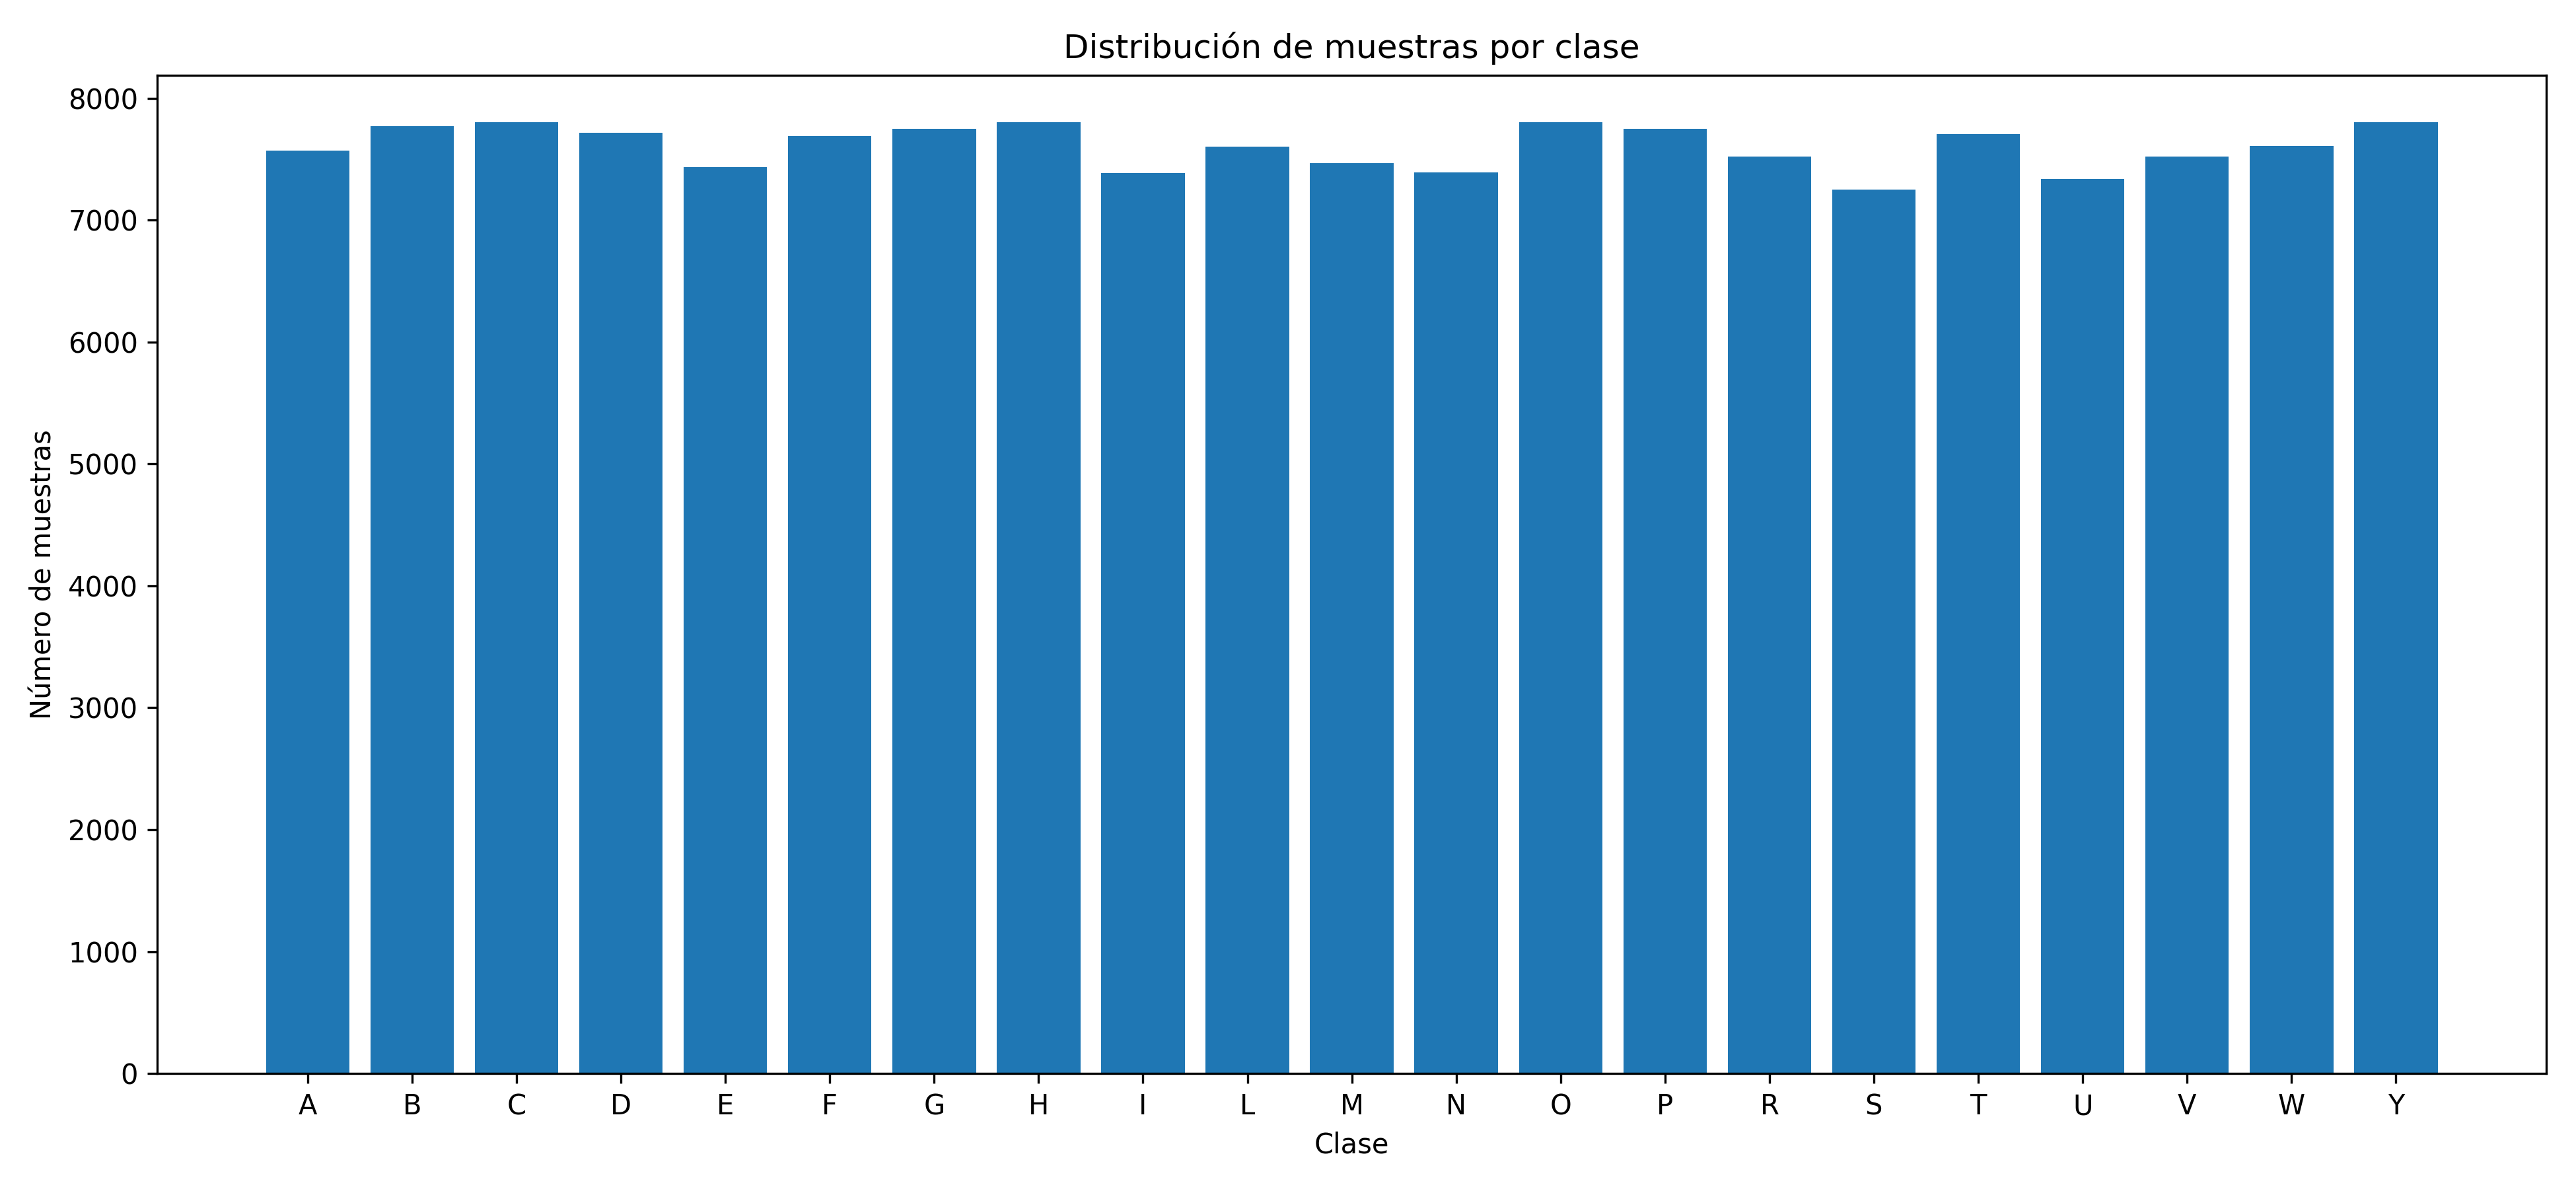
\includegraphics[width=0.95\textwidth]{images/distribucion_clases.png}
		\caption{Distribución de muestras por clase del conjunto de datos final}
		\label{fig:distribucion_dataset}
	\end{figure}
	
	Como se observa en la Figura \ref{fig:distribucion_dataset}, el conjunto de datos presenta una distribución relativamente homogénea entre las clases, manteniéndose la mayoría de ellas en un rango aproximado entre 7200 y 7800 muestras. Esta distribución equilibrada es un indicador positivo preliminar, ya que teóricamente reduce el riesgo de sesgo hacia clases mayoritarias durante la posterior etapa de entrenamiento.
	
	Desde la perspectiva del diseño del sistema, este balance uniforme permite proyectar el uso de funciones de pérdida estándar para la clasificación multiclase, tales como la entropía cruzada categórica (\textit{Categorical Cross-Entropy}) o su variante dispersa (\textit{Sparse Categorical Cross-Entropy}), las cuales basan su eficacia en la suposición de clases equitativas durante el cálculo del gradiente \cite{goodfellow2016deep}. Por otro lado la paridad en los conteos preliminares sugiere que, en principio, es viable prescindir de técnicas complejas de sobremuestreo artificial o de la implementación de funciones de pérdida modificadas, estrategias comúnmente requeridas para mitigar el sesgo en distribuciones asimétricas dentro de tareas modernas de visión artificial \cite{johnson2021survey, fujiwara2025class}.
	
	\subsection{Análisis de variabilidad geométrica y espacial}
	
	A diferencia de un análisis basado en imágenes completas, revisar la variación de los puntos de la mano requiere entender cómo cambian los números de las coordenadas dentro del lienzo de captura. Al revisar los datos del DataFrame, se observa que las coordenadas entregadas por MediaPipe ya vienen normalizadas en un rango de 0 a 1 respecto al ancho y alto de la pantalla. Sin embargo, este ajuste inicial no funciona para nuestro objetivo, ya que a nosotros no nos interesa saber la distancia ni en qué lugar de la imagen se encuentra la mano, sino conocer su configuración geométrica pura.
	
	En primer lugar, revisamos cómo cambia el tamaño de la mano en la pantalla debido a la distancia de captura. La Figura \ref{fig:histograma_escala} muestra la distribución obtenida al calcular la distancia entre la muñeca (\textit{landmark} 0) y la base del dedo medio (\textit{landmark} 9) para todo el conjunto de datos crudos.
	
	\begin{figure}[H]
		\centering
		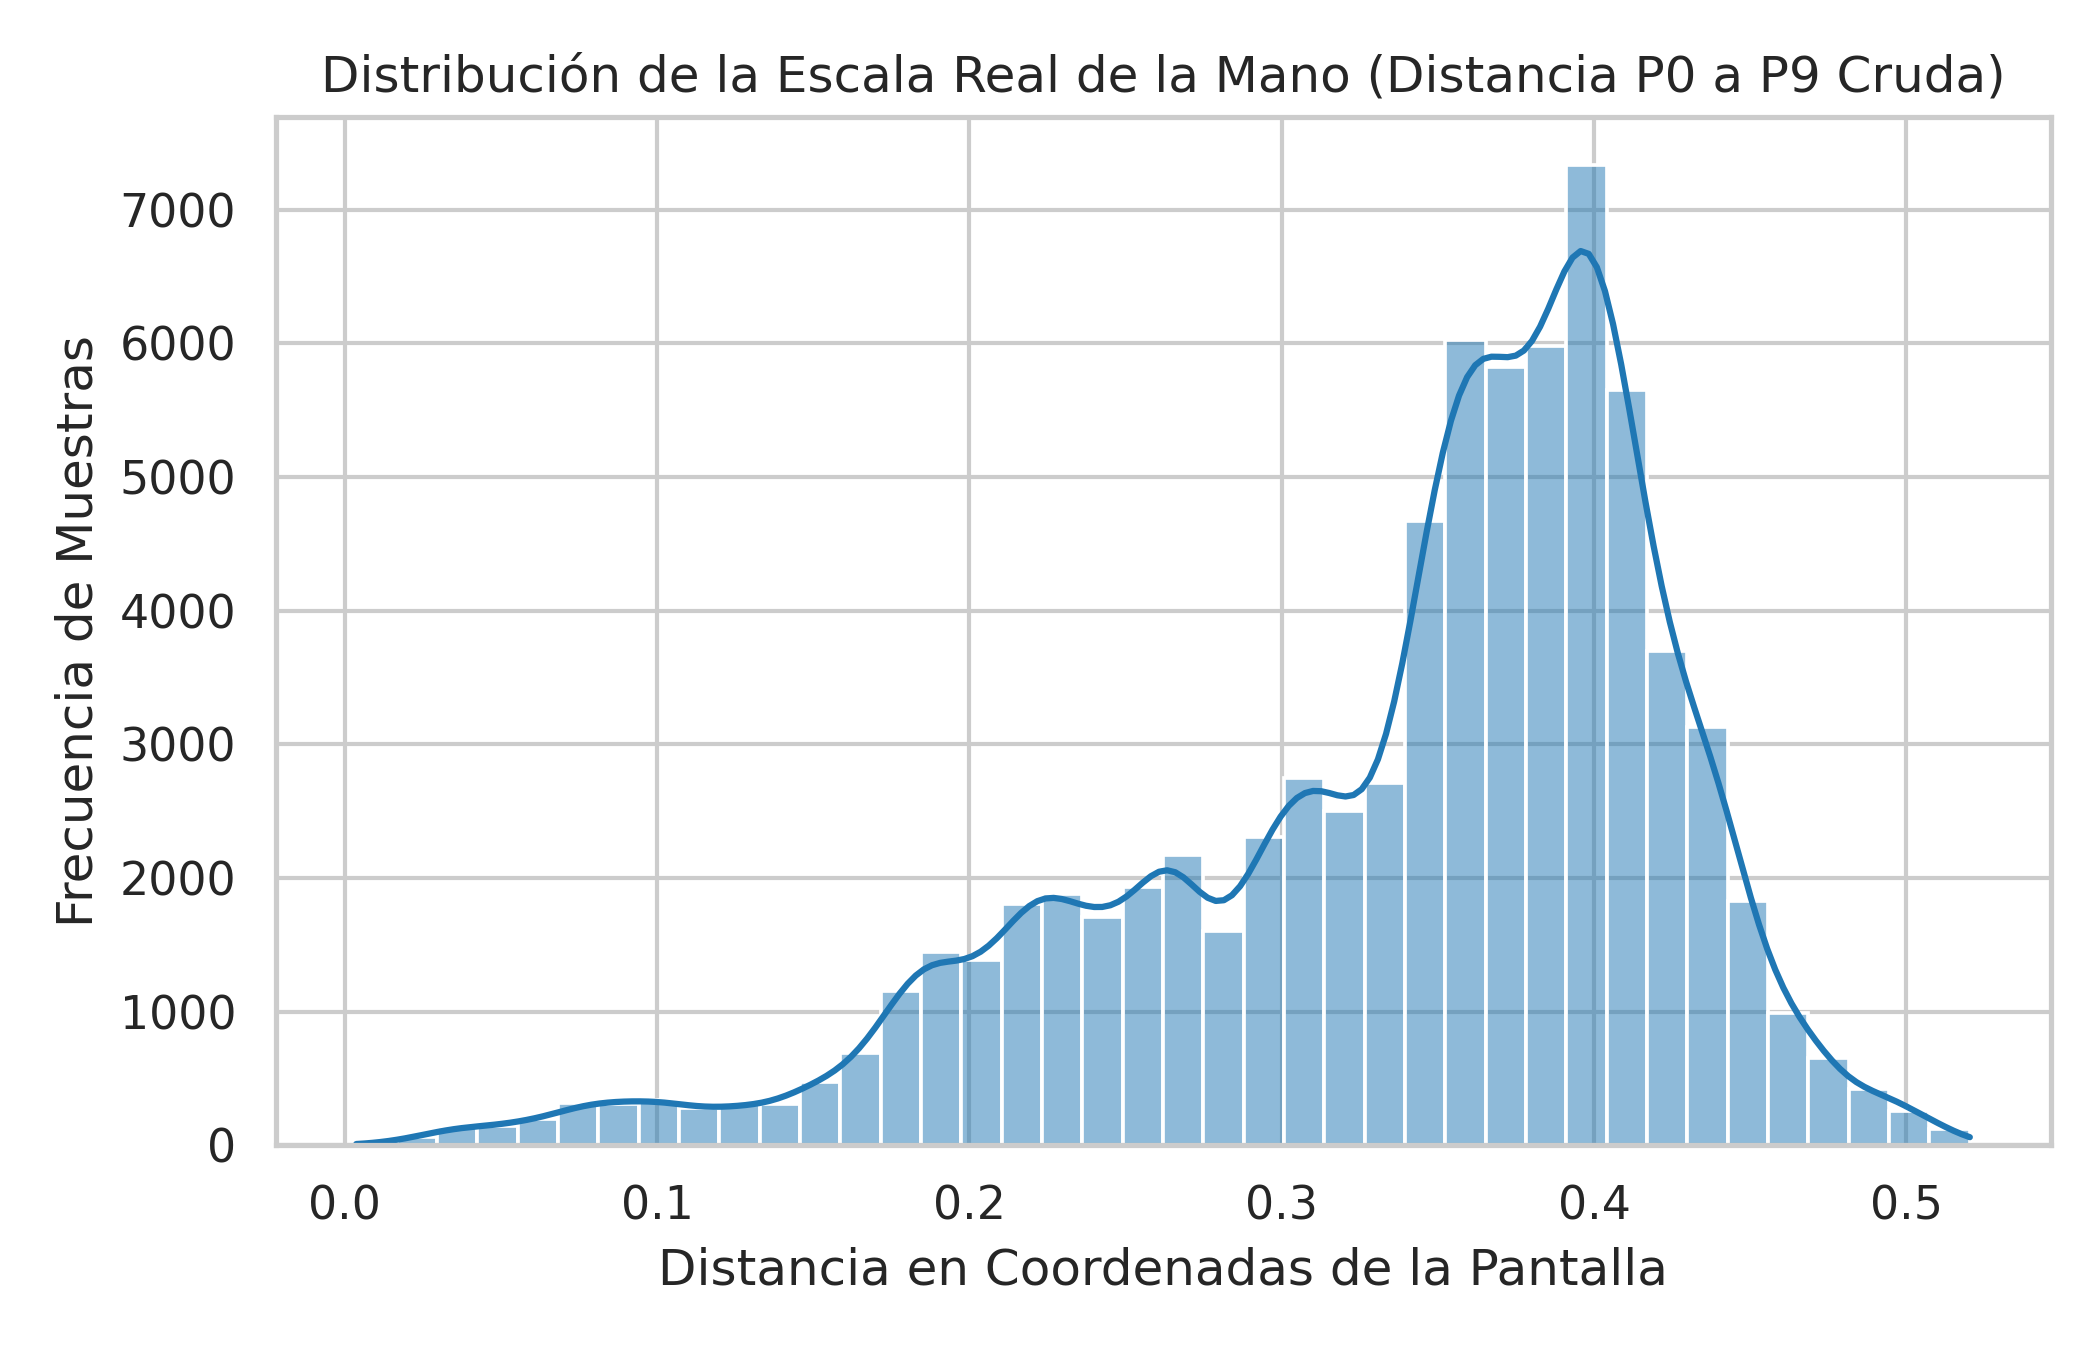
\includegraphics[width=0.90\textwidth]{images/nuevo_histograma_escala.png}
		\caption{Distribución del tamaño relativo de la palma en los datos crudos}
		\label{fig:histograma_escala}
	\end{figure}
	
	Como se ve en la Figura \ref{fig:histograma_escala}, las distancias se encuentran distribuidas entre menos de 0.1 y un máximo cercano a 0.52, concentrando la mayor parte de las muestras entre 0.35 y 0.42. Esta dispersión confirma que, aunque MediaPipe acote los valores al tamaño de la pantalla, el tamaño relativo de la mano cambia notablemente según qué tan lejos se coloque cada usuario. Si se intentara entrenar un modelo con estos datos de forma directa, el sistema podría confundir el tamaño o el encuadre con la identidad de la seña, lo que justifica la necesidad de buscar un método propio para aislar la forma de la mano independientemente de su escala.
	
	
	En segundo lugar, se utilizan diagramas de boxplot para evaluar la dispersión de las posiciones de los dedos en una misma seña tomando los datos crudos. La Figura \ref{fig:boxplot_variabilidad} muestra las distancias calculadas desde la muñeca hasta las puntas de los cinco dedos, utilizando las muestras de la letra A como escenario de prueba.
	
	\begin{figure}[H]
		\centering
		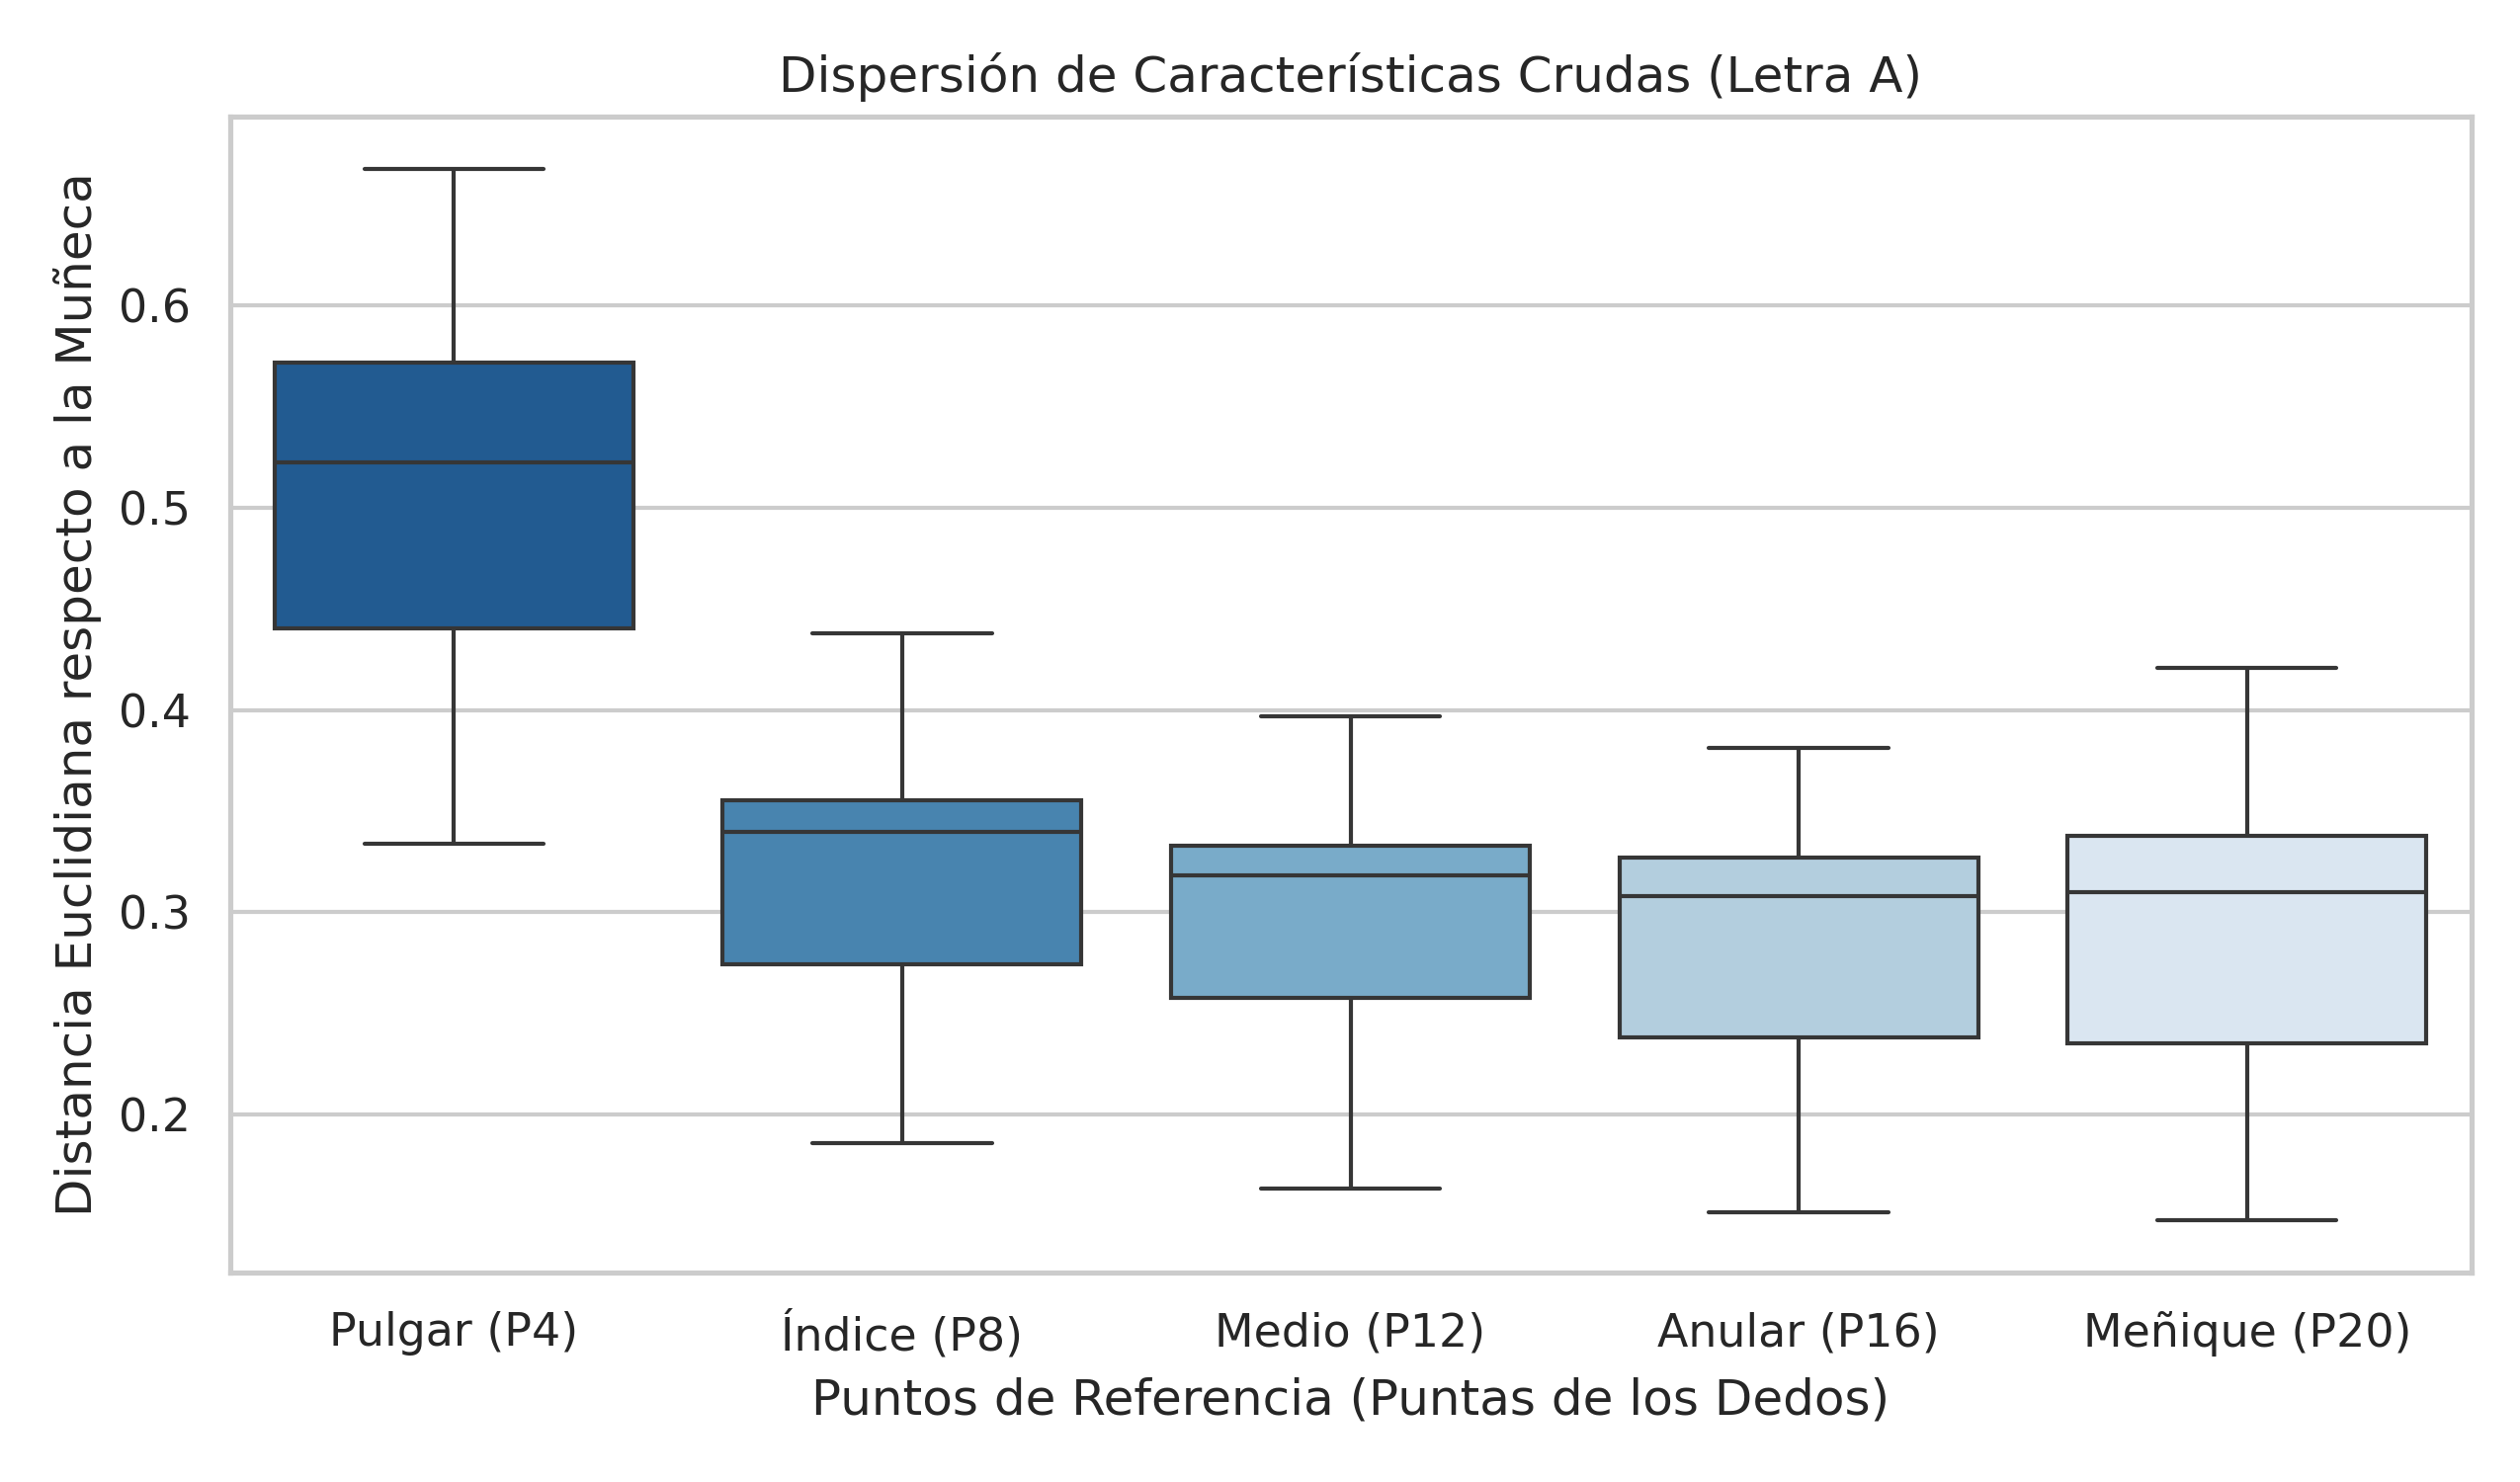
\includegraphics[width=0.85\textwidth]{images/nuevo_boxplot_letra_a.png}
		\caption{Dispersión de características crudas para la clase A}
		\label{fig:boxplot_variabilidad}
	\end{figure}
	Al analizar la Figura \ref{fig:boxplot_variabilidad}, se observa que todas las características presentan cajas amplias y bigotes extensos. El pulgar (\textit{landmark} 4), a pesar de mantener una postura fija y estirada en la seña A, muestra la caja más grande del gráfico debido a que la distancia absoluta medida en la pantalla cambia constantemente según la cercanía del usuario. Los dedos medio, anular y meñique exhiben rangos de distribución similares en la parte inferior debido a la flexión del puño. Este comportamiento confirma que las distancias absolutas en la pantalla arrastran toda la variabilidad del tamaño y encuadre de la captura, lo que reafirma la necesidad de aplicar una normalización propia centrada en la estructura interna de la mano.
	
	Para evaluar el impacto de esta variabilidad en escenarios de alta similitud morfológica, se realiza una comparación entre las señas más complejas del conjunto de datos: M, N, T, S, R y U. La Figura \ref{fig:boxplot_conflictivas} muestra la dispersión de la distancia calculada desde la muñeca hasta la punta del dedo índice (\textit{landmark} 8) para estas seis clases en su estado crudo.
	
	\begin{figure}[H]
		\centering
		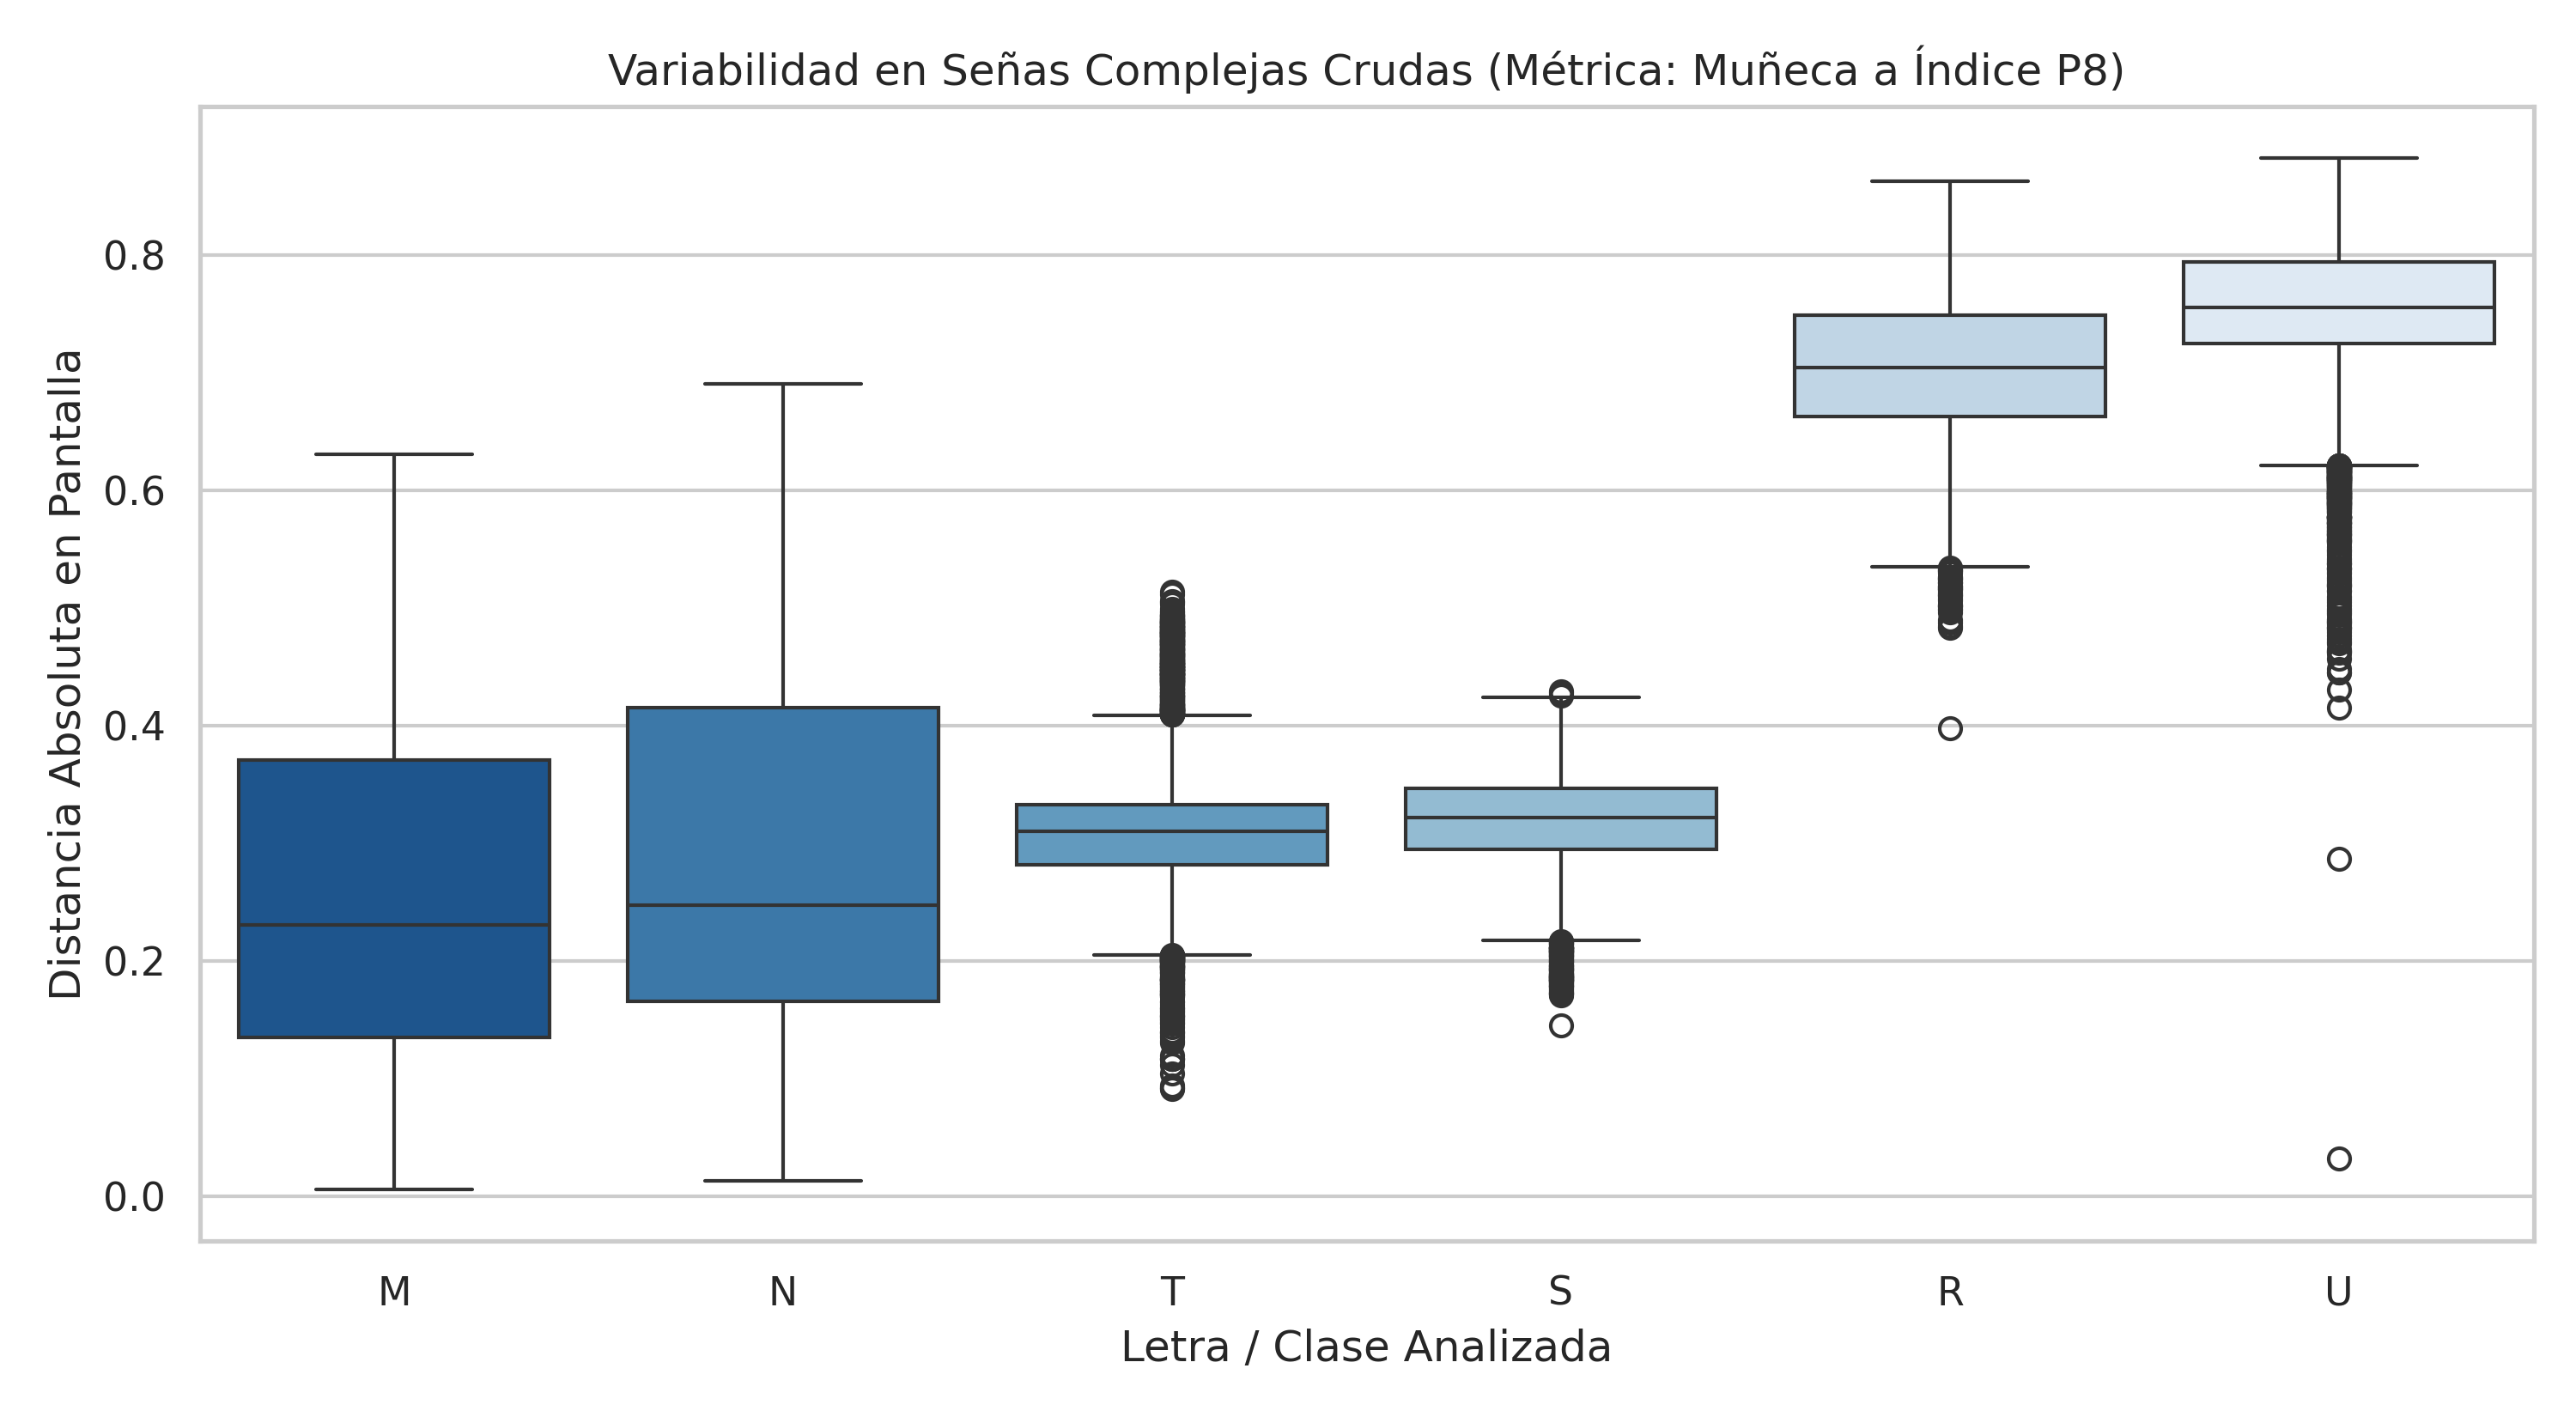
\includegraphics[width=0.85\textwidth]{images/nuevo_boxplot_conflictivas.png}
		\caption{Variabilidad en señas complejas crudas (Métrica: Muñeca a Índice P8)}
		\label{fig:boxplot_conflictivas}
	\end{figure}
	
	Los resultados de la Figura \ref{fig:boxplot_conflictivas} revelan problemas críticos para la clasificación sin un procesamiento previo:
	\begin{itemize}
		\item \textbf{Solapamiento por escala en letras cerradas (M y N):} Las letras M y N comparten casi el mismo nivel de distribución y tienen cajas muy anchas. Al depender del encuadre de la pantalla, una letra M capturada de cerca genera valores muy parecidos a una letra N capturada desde lejos, haciendo que los datos de cierta manera se encimen.
		\item \textbf{Ruido por oclusión y flexión (T y S):} Las señas T y S presentan cajas más compactas en la parte baja de la escala debido a que el índice va doblado. Sin embargo, la T muestra una enorme cantidad de puntos atípicos (\textit{outliers}) arriba y abajo, mientras que la S concentra sus errores principalmente en la parte inferior. Esto demuestra la inestabilidad que genera MediaPipe cuando el índice es obstruido por otros dedos al cerrar el puño.
		\item \textbf{Similitud de postura en letras abiertas (R y U):} Las cajas de las letras R y U se encuentran posicionadas en niveles altos y muy cercanos debido a que ambas mantienen el índice extendido. Aunque la U se encuentra ligeramente más arriba y compacta, la falta de una separación clara entre sus distribuciones provocaría errores de confusión masivos en el clasificador.
	\end{itemize}
	
	A partir de los resultados obtenidos en estas gráficas de variabilidad, queda clara la necesidad de buscar una forma de normalizar los datos para reducir el impacto de la distancia, el tamaño y la posición de los puntos. En esta etapa del proyecto, el interés principal no es saber en qué parte de la pantalla está la mano, ni qué tan lejos se encuentra el usuario o de qué tamaño es su extremidad. El objetivo real es conocer la forma exacta de la mano para poder clasificar cada seña de manera correcta.
	
	Por lo tanto los resultados de este análisis muestran que es necesario probar diferentes métodos de normalización. Esta revisión ayudará a encontrar la estrategia más estable para transformar los datos iniciales. En el desarrollo posterior se deberán hacer pruebas con distintas técnicas de centrado de puntos y cambios de escala, buscando la opción que mantenga la forma real de las señas de la LSM y reduzca el ruido provocado por los dedos ocultos.
	
	
	\subsection{Visualización del espacio de características mediante reducción dimensional}
	
	Cada muestra del conjunto de datos contiene un total de 42 dimensiones, las cuales corresponden a los ejes de las coordenadas de los puntos de la mano. Debido a que la percepción humana no puede interpretar un espacio con tantas dimensiones, resulta imposible evaluar de forma directa cómo se acomodan o se separan las diferentes clases a simple vista \cite{vandermaaten2008visualizing}. Por esta razón, es necesario realizar pruebas basadas en algoritmos de reducción de dimensiones para proyectar estos datos en una gráfica simple de dos dimensiones.
	
	En esta etapa del proyecto, esta técnica se utiliza como una herramienta de diagnóstico para revisar qué tan mezcladas o encimadas (\textit{overlapping}) quedan las señas antes de pasar al entrenamiento \cite{scikit-learn}. Ver la distribución visual de las letras permitirá entender la complejidad real del conjunto de datos crudos. Si las clases forman grupos separados y claros, se podría proponer el uso de clasificadores sencillos; por el contrario, si los datos quedan muy entrelazados debido al parecido físico de las señas, esto servirá como argumento sólido para justificar el uso de modelos más avanzados basados en redes neuronales \cite{geron2022hands}.
	
	
	\subsection{Visualización del espacio de características mediante reducción dimensional}
	
	Cada muestra del conjunto de datos contiene un total de 42 dimensiones, las cuales corresponden a los ejes de las coordenadas de los puntos de la mano. Debido a que la percepción humana no puede interpretar un espacio con tantas dimensiones, resulta imposible evaluar de forma directa cómo se acomodan o se separan las diferentes clases a simple vista \cite{vandermaaten2008visualizing}. Por esta razón, se utiliza el algoritmo de reducción de dimensiones t-SNE como una herramienta de diagnóstico visual en dos escenarios: con los datos crudos y con el dataset final preprocesado \cite{scikit-learn}.
	
	En primer lugar, se proyectó el universo de datos en su estado crudo, el cual incluye las variaciones absolutas de la pantalla. Los resultados de esta primera prueba se muestran en la Figura \ref{fig:tsne_completo}.
	
	\begin{figure}[H]
		\centering
		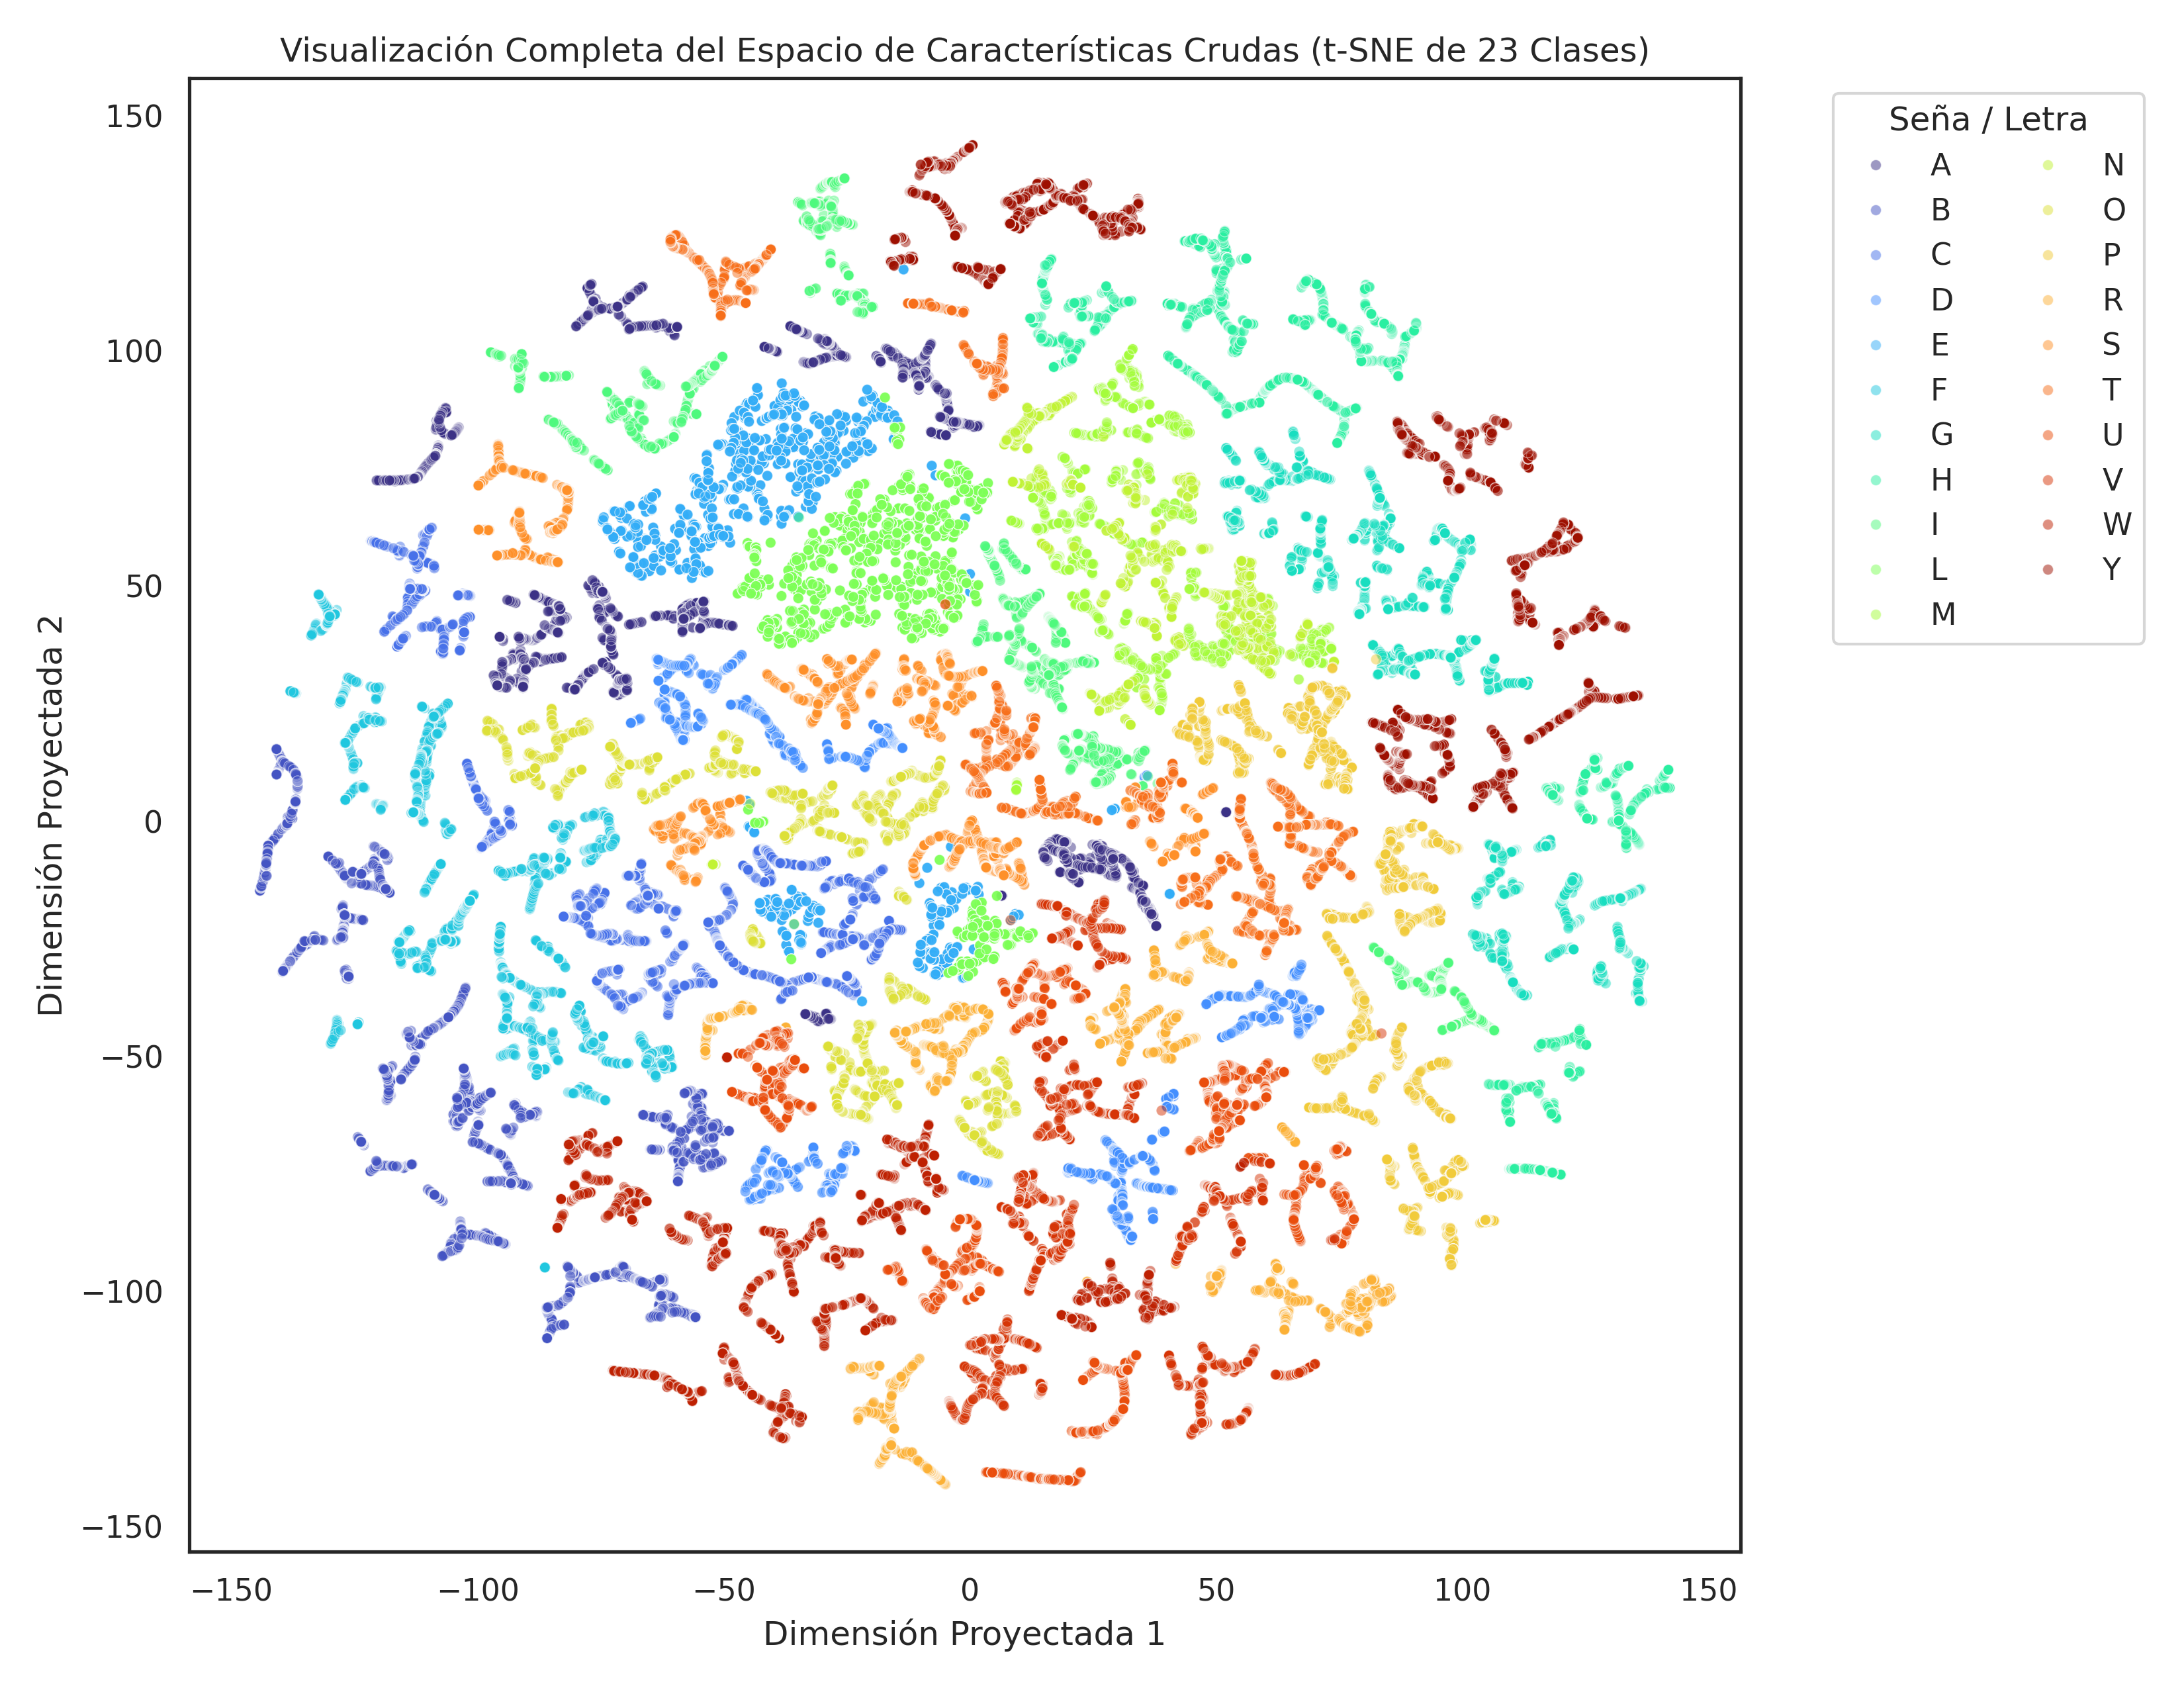
\includegraphics[width=0.85\textwidth]{images/tsne_dataset_completo.png}
		\caption{Visualización del espacio de características crudas mediante t-SNE}
		\label{fig:tsne_completo}
	\end{figure}
	
	Al analizar la estructura de la Figura \ref{fig:tsne_completo}, se observa una masa central amorfa donde clases como M, N, O, S y T se encuentran entrelazadas en algunas zonas. Asimismo, señas como B, C, L, W y Y se extienden hacia las orillas en forma de ramificaciones alargas. Este comportamiento confirma que los datos crudos arrastran toda la variabilidad de la distancia y el encuadre de la cámara, diluyendo las fronteras reales entre las letras de la LSM.
	
	Para comprobar la efectividad de las etapas de limpieza, se volvió a ejecutar el mismo algoritmo utilizando el dataset de 150000 muestras totalmente normalizado y preprocesado, listo para la etapa de entrenamiento. El resultado de esta proyección se observa en la Figura \ref{fig:tsne_normalizado}.
	
	\begin{figure}[H]
		\centering
		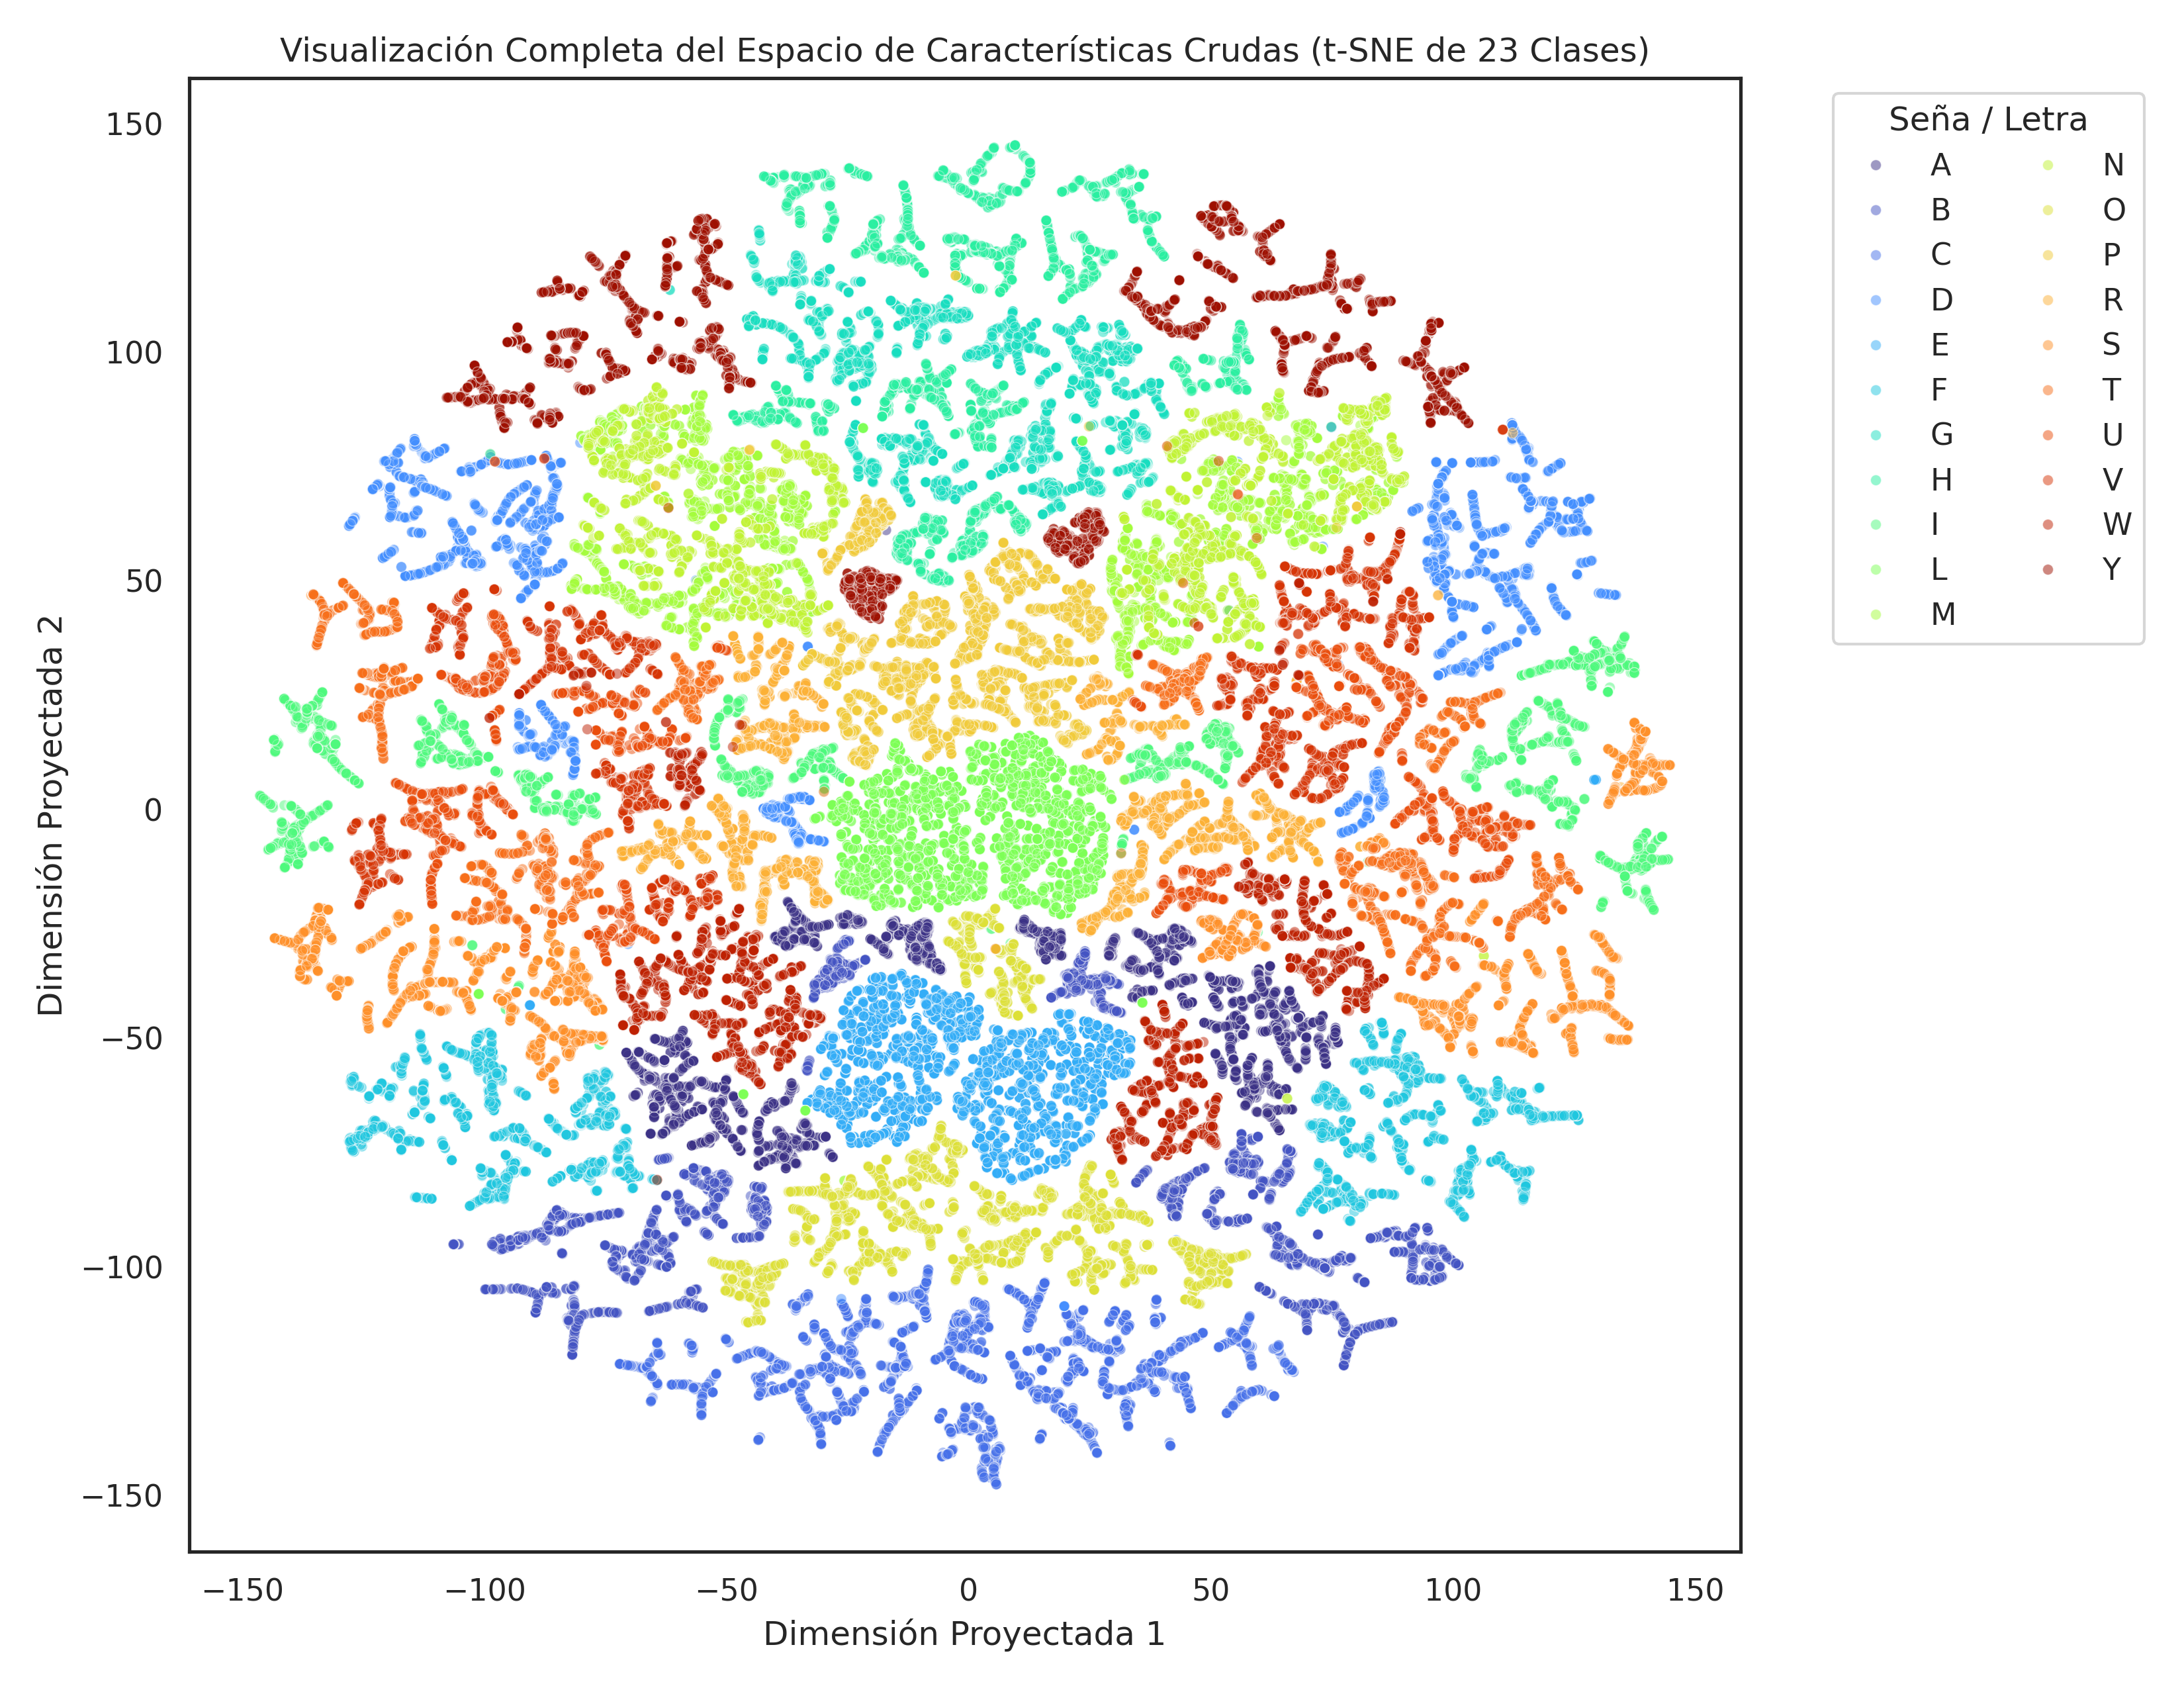
\includegraphics[width=0.85\textwidth]{images/tsne_dataset_completo_normalizadas.png}
		\caption{Visualización del espacio de características normalizadas listo para entrenamiento}
		\label{fig:tsne_normalizado}
	\end{figure}
	
	Al comparar la Figura \ref{fig:tsne_normalizado} con la proyección cruda anterior, se identifican cambios metodológicos fundamentales:
	\begin{itemize}
		\item \textbf{Compactación de clusters:} Las ramificaciones alargadas redujeron considerablemente. Al eliminar el factor de escala provocado por la distancia del usuario a la cámara, las muestras de una misma configuración geométrica se agruparon de forma densa y ordenada.
		\item \textbf{Estructura geométrica definida:} Los datos se reacomodaron en agrupaciones mas grandes y continuas que reflejan la transición física real entre las posturas de los dedos.
		\item \textbf{Complejidad no lineal persistente:} A pesar de la notable limpieza y orden en los datos, las clases siguen compartiendo fronteras sumamente complejas. En la región central y en las zonas periféricas se aprecia cómo clusters de diferentes colores se rodean y colindan directamente entre sí sin llegar a separarse de forma aislada.
	\end{itemize}
	
	La distribución visual obtenida en el escenario preprocesado demuestra  que el problema de reconocimiento de la LSM no es linealmente separable. Intentar resolver este sistema mediante clasificadores estadísticos simples o modelos lineales provocaría un porcentaje de error en la aplicación móvil, ya que estos algoritmos son incapaces de trazar límites curvos y complejos en zonas de alta colindancia como las que exhiben algunas letras  letras.
	
	La comparación de ambos espacios de características justifica la selección tecnológica de este proyecto: el algoritmo de normalización local propuesto es indispensable para ordenar el espacio numérico, mientras que el uso de una arquitectura basada en redes neuronales artificiales será la mejor opción, ya que es la única herramienta capaz de aprender fronteras no lineales de alta complejidad para asegurar una clasificación robusta y precisa en el dispositivo final \cite{geron2022hands}.
	
	\section{Conclusiones del análisis exploratorio}
	
	A partir del análisis exploratorio, se determina que el éxito del clasificador embebido en un dispositivo móvil no depende de buscar un modelo de aprendizaje profundo exageradamente grande o complejo. El verdadero rendimiento del sistema radica en encontrar una configuración de normalización adecuada combinada con un ajuste correcto de hiperparámetros para entrenar la red neuronal.
	
	Los datos crudos muestran problemas en su estructura que exigen realizar pruebas rigurosas. A continuación, se detallan los retos del entorno real y la ruta de trabajo justificada por las gráficas estadísticas anteriores.
	
	\subsection{Caminos para la experimentación y normalización de datos}
	
	Los resultados del histograma de escala y las proyecciones t-SNE demostraron que la normalización general mediante cajas delimitadoras (\textit{bounding boxes}) ayuda a que los datos no se salgan de la pantalla, pero no es suficiente. Este método deforma las proporciones de la mano cuando el usuario abre o cierra el puño. Por lo tanto, las siguientes pruebas deben enfocarse en quitar la dependencia de la pantalla y diseñar un forma de normalizar basado únicamente en la estructura de la mano, evaluando tres estrategias :
	
	\begin{itemize}
		\item \textbf{Uso de un punto de anclaje local:} En lugar de usar los extremos de la pantalla, las pruebas deben orientarse a usar un punto fijo de la mano como el centro del mapa de coordenadas. El punto ideal es la muñeca (\textit{landmark} 0) o la base del dedo medio (\textit{landmark} 9). Al restar la posición de este punto central a todos los demás, se calcula un vector de desplazamiento local que elimina el problema de si la mano se mueve de lugar en la pantalla.
		\item \textbf{Ajuste de escala por el tamaño de la palma:} Para solucionar los cambios de tamaño provocados por la distancia, se debe probar un factor de división basado en una distancia de la mano que casi nunca cambie, como la línea que va de la muñeca a la base del dedo medio ($||P_9 - P_0||$). Al dividir todas las coordenadas entre esta distancia, el tamaño de la mano se estandariza sin importar si el usuario está muy cerca o lejos de la cámara del celular.
		\item \textbf{Corrección por inclinación de la mano:} El análisis de los datos crudos asume que la mano siempre está derecha. En el uso real, la gente inclina la muñeca de forma natural. Es necesario experimentar con fórmulas de rotación geométrica basadas en el ángulo de la palma, buscando que los datos finales sean los mismos aunque el usuario gire un poco la mano o el celular.
	\end{itemize}
	
	\subsection{Retos del entorno real y problemas físicos}
	
	Llevar un traductor de señas a un teléfono móvil introduce variables del mundo físico que pueden alterar los números que recibe el sistema. Las gráficas de boxplot mostraron que MediaPipe mete ruido cuando se presentan ciertas condiciones, las cuales representan los principales retos de ingeniería para el proyecto:
	
	\begin{itemize}
		\item \textbf{Dedos ocultos o tapados entre sí:} Este es el reto más difícil en las señas que llevan el puño cerrado o los dedos cruzados como M, N, T y S. Cuando un dedo tapa a otro frente a la cámara, el sistema de MediaPipe pierde la vista directa y empieza a calcular la posición del punto oculto mediante estimaciones. Esto genera datos erróneos y saltos bruscos en las coordenadas (los puntos atípicos u \textit{outliers} que vimos en las gráficas). Las pruebas con el modelo deben ser capaces de absorber este ruido para evitar fallas en la aplicación.
		\item \textbf{Señas que se parecen físicamente:} El t-SNE del dataset normalizado dejó claro que letras como R y U, o M y N, se quedan pegadas en el mapa porque la postura de la mano es casi la misma. El enfoque de los experimentos no debe ser solo separar grupos grandes, sino lograr que el sistema detecte los detalles más pequeños, como la separación milimétrica entre las puntas de los dedos o el cruce exacto del pulgar. Si el procesamiento no resalta estas diferencias, el modelo final va a confundir estas letras constantemente.
		\item \textbf{Cambios de luz y ruido en la cámara:} Las cámaras de los celulares cambian su configuración dependiendo de la luz del cuarto. Cuando hay poca iluminación, la imagen pierde nitidez y los bordes de los dedos se ven borrosos, haciendo que los puntos de MediaPipe tiemblen de un cuadro a otro aunque la mano esté quieta. Este temblor en las coordenadas se debe controlar mediante filtros matemáticos antes de mandar los datos al clasificador.
		\item \textbf{Ángulo de la toma y perspectiva:} El usuario común no va a sostener el celular en una posición perfecta frente a su rostro. Si el teléfono se inclina, los dedos estirados se verán más cortos en la pantalla de lo que realmente son debido a la perspectiva. Para superar esto, las transformaciones matemáticas en el preprocesamiento deben aprovechar la coordenada de profundidad relativa que ofrece el sensor para corregir la postura en un entorno tridimensional virtual.
	\end{itemize}
	
	
	La evidencia que dejaron las gráficas cierra por completo la posibilidad de usar reglas fijas o algoritmos estadísticos simples. El mapa de las 21 letras, incluso estando normalizado y limpio, muestra que las fronteras entre las señas de la LSM no son líneas rectas, sino curvas y pliegues complejos donde unas clases rodean a otras, especialmente en el grupo de M, N, S y T.
	
	Los principales retos serán:
	
	1. Crear un proceso de limpieza de características propio y local que unifique el tamaño y rotación de la mano, eliminando el ruido de la pantalla antes de que los datos lleguen al clasificador.
	2. Implementar un MLP entrenado específicamente para aprender estas fronteras curvas y complejas que los modelos lineales sencillos no pueden resolver.
	
	Esta combinación asegura que las pequeñas diferencias entre las señas difíciles puedan separarse con alta precisión, consumiendo muy pocos recursos del teléfono al exportar el modelo final en formato TensorFlow Lite.
	
	
	\section{Consideraciones de uso y privacidad}
	
	VisionLSM es un prototipo académico y experimental desarrollado como parte de un trabajo terminal del Instituto Politécnico Nacional, cuyo objetivo principal consiste en desarrollar un prototipo para reconocimiento de señas estáticas de la LSM en dispositivos móviles Android mediante visión por computadora.
	
	Debido a la naturaleza experimental del proyecto, la aplicación se encuentra en una etapa de desarrollo y validación, por lo que su funcionamiento puede presentar variaciones dependiendo de las condiciones de uso, el dispositivo empleado y el entorno de captura. El sistema fue diseñado con fines académicos, de investigación y demostración tecnológica, por lo que no debe considerarse un producto comercial ni un sistema definitivo para comunicación asistida.
	
	Actualmente la aplicación no se encuentra distribuida mediante Google Play Store debido a que se trata de un prototipo en fase de evaluación académica. Es por eso que la instalación de la aplicación debe realizarse manualmente mediante un archivo .apk proporcionado por los desarrolladores o responsables del proyecto.
	
	El usuario reconoce y acepta que la instalación de aplicaciones externas mediante archivos .apk puede requerir la habilitación de permisos especiales dentro del sistema operativo Android, así como la aceptación de configuraciones relacionadas con la instalación de aplicaciones provenientes de fuentes externas a Google Play Store.
	
	Asimismo, el usuario acepta que el uso de la aplicación se realiza bajo su propia responsabilidad. Los desarrolladores no garantizan un funcionamiento libre de errores ni una precisión absoluta en las inferencias realizadas por el sistema, debido a las limitaciones inherentes a los modelos de inteligencia artificial y a las condiciones variables presentes durante el reconocimiento de señas. De igual forma el prototipo no sustituye la labor de intérpretes profesionales y certificados de LSM ni debe considerarse un sistema oficial de traducción o asistencia para la comunicación.
	
	El uso del prototipo implica la aceptación de las consideraciones técnicas, limitaciones operativas y condiciones descritas en el presente documento.

	

	\section{Términos y condiciones de uso}
	
	\subsection{Aceptación de los términos}
	
	El uso, instalación o acceso a la aplicación VisionLSM implica que el usuario ha leído, comprendido y aceptado los presentes términos y condiciones de uso, así como las disposiciones descritas en el aviso de privacidad incluido en el presente documento.
	
	En caso de que el usuario no esté de acuerdo con alguna de las condiciones establecidas, deberá abstenerse de instalar o utilizar la aplicación.
	
	Asimismo, el usuario reconoce que la aplicación corresponde a un prototipo académico y experimental, por lo que acepta las limitaciones técnicas, operativas y funcionales propias del sistema, así como el uso de la aplicación bajo su propia responsabilidad.
	
	\subsection{Uso permitido}
	
	El usuario se compromete a utilizar la aplicación únicamente con fines lícitos, éticos y compatibles con los objetivos académicos y tecnológicos del proyecto.
	
	Se permite el uso de la aplicación para:
	
	\begin{itemize}
		\item Actividades académicas y educativas.
		
		\item Pruebas experimentales relacionadas con el reconocimiento de señas.
		
		\item Evaluación y demostración del funcionamiento del prototipo.
		
		\item Actividades de investigación orientadas al análisis de modelos de inteligencia artificial y visión por computadora.
		
		\item Apoyo experimental a procesos de comunicación mediante reconocimiento de señas.
	\end{itemize}
	
	El uso de la aplicación deberá realizarse respetando en todo momento la privacidad, integridad y derechos de terceros.
	
	\subsection{Restricciones de uso}
	
	Queda prohibido utilizar la aplicación para actividades contrarias a la ley, la ética o los objetivos académicos para los cuales fue desarrollada.
	
	El usuario se compromete a no:
	
	\begin{itemize}
		\item Modificar, descompilar, alterar o intentar vulnerar el funcionamiento interno de la aplicación sin autorización de los desarrolladores.
		
		\item Utilizar el sistema con fines ilícitos, fraudulentos o que puedan afectar a terceros.
		
		\item Emplear la aplicación para actividades discriminatorias, ofensivas o que vulneren derechos humanos.
		
		\item Utilizar la aplicación como sustituto de servicios profesionales, intérpretes certificados o mecanismos oficiales de comunicación.
		
		\item Intentar acceder, manipular o alterar componentes internos relacionados con el modelo de inteligencia artificial, procesamiento de imágenes o funcionamiento del sistema.
		
		\item Distribuir versiones modificadas de la aplicación sin autorización expresa de los desarrolladores.
	\end{itemize}
	
	Cualquier uso indebido de la aplicación será responsabilidad exclusiva del usuario.
	
	\subsection{Limitaciones del sistema}
	
	El usuario reconoce que VisionLSM corresponde a un prototipo experimental basado en modelos de inteligencia artificial y visión por computadora, por lo que el sistema puede presentar errores, variaciones o limitaciones durante el reconocimiento de señas.
	
	La precisión del reconocimiento puede verse afectada por diferentes factores, entre ellos:
	
	\begin{itemize}
		\item Condiciones de iluminación insuficientes o excesivas.
		
		\item Fondos visualmente complejos o con múltiples objetos.
		
		\item Oclusiones parciales o total de la mano.
		
		\item Posicionamiento incorrecto respecto a la cámara.
		
		\item Distancias inadecuadas entre la mano y el dispositivo móvil.
		
		\item Movimientos rápidos o inestables durante la captura.
		
		\item Variaciones físicas entre usuarios, tales como tamaño de mano, orientación o forma de realizar las señas.
		
		\item Limitaciones inherentes al modelo de inteligencia artificial utilizado.
	\end{itemize}
	
	Con base en lo anterior los resultados generados por la aplicación deben considerarse de carácter orientativo y experimental, por lo que no se garantiza una precisión absoluta en todas las condiciones de uso.
	
	El sistema no sustituye intérpretes profesionales de Lengua de Señas Mexicana ni debe utilizarse como herramienta oficial de traducción o asistencia crítica para la comunicación.
	
	\subsection{Disponibilidad del servicio}
	
	Dado que VisionLSM corresponde a un prototipo académico y experimental en fase de desarrollo y evaluación tecnológica, no se garantiza la disponibilidad permanente del sistema ni el funcionamiento ininterrumpido de la aplicación en todos los dispositivos móviles Android.
	
	La compatibilidad del sistema puede variar dependiendo de factores como:
	
	\begin{itemize}
		\item Versión del sistema operativo Android.
		
		\item Capacidades de hardware del dispositivo.
		
		\item Calidad y resolución de la cámara.
		
		\item Recursos disponibles del sistema, tales como memoria RAM y capacidad de procesamiento.
		
		\item Configuraciones internas del dispositivo móvil.
	\end{itemize}
	
	Asimismo, los desarrolladores podrán suspender temporalmente el funcionamiento del sistema, realizar modificaciones o actualizar componentes de la aplicación con fines académicos, de mantenimiento, corrección de errores o mejora del prototipo.
	
	Debido a la naturaleza experimental del proyecto, no se garantiza compatibilidad absoluta, disponibilidad continua ni estabilidad total en todas las condiciones de uso.
	
	\subsection{Responsabilidad del usuario}
	
	El usuario es responsable del uso que realice de la aplicación, así como de la instalación del archivo .apk en su dispositivo móvil y de la configuración de los permisos necesarios para el funcionamiento del sistema.
	
	Antes de utilizar la aplicación, el usuario deberá otorgar permiso explícito para el acceso a la cámara del dispositivo, reconociendo que dicho recurso es indispensable para el funcionamiento del sistema de reconocimiento de señas.
	
	El usuario también acepta utilizar la aplicación en entornos adecuados y seguros, respetando en todo momento la privacidad, integridad y derechos de terceros. Los desarrolladores no se hacen responsables por el uso indebido de la aplicación, ni por posibles afectaciones derivadas de configuraciones incorrectas, incompatibilidades del dispositivo o interpretaciones erróneas generadas por el sistema.
	
	Debido a que la instalación se realiza mediante un archivo .apk externo y no a través de Google Play Store, el usuario reconoce y acepta los riesgos asociados a la instalación manual de aplicaciones provenientes de fuentes externas, así como la responsabilidad derivada de habilitar los permisos correspondientes dentro del sistema operativo Android.
	
	\subsection{Propiedad intelectual}
	
	El código fuente, arquitectura de software, modelos de inteligencia artificial, documentación, diseño de interfaces y demás componentes desarrollados para VisionLSM forman parte del trabajo terminal realizado en el Instituto Politécnico Nacional con fines académicos y de investigación tecnológica.
	
	Todos los elementos desarrollados dentro del proyecto se encuentran protegidos por las disposiciones aplicables en materia de propiedad intelectual y derechos de autor. La reproducción, distribución, modificación o utilización total o parcial del sistema con fines comerciales requerirá autorización expresa de los autores del proyecto.
	
	El uso académico y demostrativo de la aplicación no otorga al usuario derechos de propiedad sobre el software, los modelos de inteligencia artificial, la documentación técnica ni sobre cualquier componente relacionado con el desarrollo del prototipo.
	
	Las bibliotecas, frameworks y herramientas de terceros utilizadas durante el desarrollo del sistema conservan los derechos y licencias establecidos por sus respectivos propietarios y desarrolladores.
	
	\section{Aviso de privacidad}

	\subsection{Información recopilada}
	
	Para el funcionamiento de VisionLSM, la aplicación puede acceder a determinados recursos y datos básicos del dispositivo móvil, necesarios para ejecutar el sistema de reconocimiento de señas.
	
	La aplicación solicita acceso a:
	
	\begin{itemize}
		\item Cámara del dispositivo móvil.
		
		\item Información básica relacionada con el funcionamiento del sistema operativo y capacidades generales del dispositivo.
	\end{itemize}
	
	El acceso a la cámara es indispensable para capturar temporalmente imágenes durante el proceso de detección y reconocimiento de señas realizadas por el usuario.
	
	Cierta información técnica del dispositivo puede ser utilizada de manera limitada con fines relacionados con compatibilidad, ejecución del sistema y funcionamiento general de la aplicación. En ningún caso esta información es utilizada con fines comerciales, publicitarios o de rastreo del usuario.
	
	\subsection{Datos procesados}
	
	Durante el funcionamiento de VisionLSM, el sistema realiza el procesamiento temporal de información necesaria para ejecutar el reconocimiento y clasificación de señas.
	
	Los datos procesados por la aplicación pueden incluir:
	
	\begin{itemize}
		\item Imágenes capturadas temporalmente por la cámara del dispositivo móvil durante el reconocimiento.
		
		\item Coordenadas y puntos de referencia de la mano obtenidos mediante algoritmos de detección y seguimiento.
		
		\item Resultados generados por el modelo de inteligencia artificial, tales como letras o señas reconocidas y niveles de confianza asociados a la inferencia.
	\end{itemize}
	
	La información procesada es utilizada exclusivamente para ejecutar las funciones de reconocimiento de señas, evaluación del desempeño del sistema y funcionamiento general del prototipo.
	
	El procesamiento de esta información se realiza de manera temporal y únicamente durante la interacción activa del usuario con la aplicación.
	
	\subsection{Datos no recopilados}
	
	VisionLSM no recopila, almacena ni comparte de manera permanente información personal sensible del usuario durante el funcionamiento normal de la aplicación.
	
	La aplicación no solicita ni procesa:
	
	\begin{itemize}
		\item Información bancaria o financiera.
		
		\item Contraseñas o credenciales de acceso.
		
		\item Ubicación geográfica mediante GPS.
		
		\item Información de contactos personales.
		
		\item Mensajes privados o contenido externo al funcionamiento de la aplicación.
		
		\item Fotografías o videos almacenados permanentemente en el dispositivo.
		
		\item Datos biométricos persistentes orientados a identificación personal.
	\end{itemize}
	
	Las imágenes capturadas temporalmente durante el reconocimiento de señas no son almacenadas de manera permanente durante el uso normal del sistema.
	
	\subsection{Procesamiento local}
	
	VisionLSM realiza el procesamiento principal de imágenes y la ejecución del modelo de inteligencia artificial directamente en el dispositivo móvil del usuario, mediante técnicas de inferencia local.
	
	Esto significa que las imágenes capturadas por la cámara y los datos generados durante el reconocimiento de señas son procesados principalmente dentro del propio dispositivo, reduciendo la necesidad de transferir información hacia servidores externos o servicios en la nube.
	
	El enfoque de procesamiento local permite:
	
	\begin{itemize}
		\item Disminuir la exposición de información visual del usuario.
		
		\item Reducir riesgos asociados a la transferencia de datos.
		
		\item Mejorar la privacidad durante el uso de la aplicación.
		
		\item Permitir el funcionamiento del sistema sin conexión permanente a internet.
	\end{itemize}
	
	Durante el funcionamiento normal de la aplicación, las inferencias realizadas por el modelo de clasificación no requieren el envío continuo de imágenes, videos o datos personales a plataformas externas para ejecutar el reconocimiento de señas.
	
	
	\subsection{Cumplimiento normativo}
	
	El tratamiento y procesamiento de la información dentro de VisionLSM se realiza considerando principios de privacidad, confidencialidad y minimización de datos establecidos en la legislación mexicana aplicable en materia de protección de datos personales, especificamente en la Ley Federal de Protección de Datos Personales en Posesión de los Particulares (LFPDPPP).
	
	Debido a la naturaleza académica y experimental del proyecto, los datos procesados por la aplicación son utilizados exclusivamente con fines relacionados con el funcionamiento del sistema.
	
	El diseño de la aplicación considera medidas orientadas a reducir la exposición innecesaria de información del usuario, priorizando el procesamiento local de imágenes, la minimización de datos procesados y la no recopilación permanente de información personal sensible durante el funcionamiento normal del sistema.

		
	\subsection{Aceptación del aviso de privacidad}
	
	El uso, instalación o acceso a la aplicación VisionLSM implica que el usuario ha leído, comprendido y aceptado las disposiciones establecidas en el presente aviso de privacidad.
	
	Asimismo, el usuario reconoce y acepta que la aplicación requiere acceso temporal a la cámara del dispositivo móvil para ejecutar las funciones de reconocimiento de señas descritas en el presente manual.
	
	En caso de que el usuario no esté de acuerdo con las condiciones relacionadas con el tratamiento y procesamiento de la información descritas en este documento, deberá abstenerse de instalar o utilizar la aplicación.
	
	El consentimiento otorgado por el usuario se limita exclusivamente al funcionamiento académico, experimental y tecnológico del prototipo desarrollado dentro del presente Trabajo Terminal.
	
	
	


% =========================
% BIBLIOGRAFIA
% =========================
	\backmatter
	\printbibliography[title={Referencias},heading=bibintoc]

\end{document}
